%\title{深度学习中文翻译版}
\documentclass[a4paper,11pt]{book}

\usepackage{xeCJK}
%\setCJKmainfont[BoldFont=STSong, ItalicFont=STKaiti]{STSong}
%\setCJKsansfont[BoldFont=STHeiti]{STXihei}
%\setCJKmonofont{STFangsong}
\usepackage{enumerate}
\usepackage{caption}
\usepackage{bm}
\setlength{\parskip}{1em}

\usepackage[T1]{fontenc}
\usepackage[utf8]{inputenc}
\usepackage{lmodern}
%%%%%%%%%%%%%%%%%%%%%%%%%%%%%%%%%%%%%%%%%%%%%%%%%%%%%%%%%
% Source: http://en.wikibooks.org/wiki/LaTeX/Hyperlinks %
%%%%%%%%%%%%%%%%%%%%%%%%%%%%%%%%%%%%%%%%%%%%%%%%%%%%%%%%%
\usepackage{hyperref}
\usepackage{graphicx}
\usepackage[english]{babel}

% *** Editing Commands ***
\usepackage{xcolor}
\usepackage[normalem]{ulem} % use normalem to protect \emph
\newcommand\add{\bgroup\markoverwith
  {\textcolor{green}{\rule[-.5ex]{.1pt}{2.5ex}}}\ULon}
\newcommand\remove{\bgroup\markoverwith
  {\textcolor{red}{\rule[-.5ex]{.1pt}{2.5ex}}}\ULon}
\newcommand{\consider}{\bgroup\markoverwith
  {\textcolor{yellow}{\rule[-.5ex]{.1pt}{2.5ex}}}\ULon}
  
% *** URL Support ***
\usepackage{url}

% *** Math Symbols Support ***
\usepackage{amsfonts}
\usepackage{amssymb}

% *** Equation Number ***
\usepackage{amsmath}
\numberwithin{equation}{chapter}

\newenvironment{dedication}
{
   \cleardoublepage
   \thispagestyle{empty}
   \vspace*{\stretch{1}}
   \hfill\begin{minipage}[t]{0.66\textwidth}
   \raggedright
}
{
   \end{minipage}
   \vspace*{\stretch{3}}
   \clearpage
}

%%%%%%%%%%%%%%%%%%%%%%%%%%%%%%%%%%%%%%%%%%%%%%%%
% Chapter quote at the start of chapter        %
% Source: http://tex.stackexchange.com/a/53380 %
%%%%%%%%%%%%%%%%%%%%%%%%%%%%%%%%%%%%%%%%%%%%%%%%
\makeatletter
\renewcommand{\@chapapp}{}% Not necessary...
\newenvironment{chapquote}[2][2em]
  {\setlength{\@tempdima}{#1}%
   \def\chapquote@author{#2}%
   \parshape 1 \@tempdima \dimexpr\textwidth-2\@tempdima\relax%
   \itshape}
  {\par\normalfont\hfill--\ \chapquote@author\hspace*{\@tempdima}\par\bigskip}
\makeatother

%%%%%%%%%%%%%%%%%%%%%%%%%%%%%%%%%%%%%%%%%%%%%%%%%%%
% First page of book which contains 'stuff' like: %
%  - Book title, subtitle                         %
%  - Book author name                             %
%%%%%%%%%%%%%%%%%%%%%%%%%%%%%%%%%%%%%%%%%%%%%%%%%%%



\title{\Huge \textbf{深度学习} }
% Author
\author{\textsc{Ian Goodfellow} \\ \textsc{Yoshua Bengio} \\ \textsc{Aaron Courville}}
\begin{document}

\frontmatter
\maketitle
\begin{itemize}
\item 
\end{itemize}

\tableofcontents
\listoffigures
\listoftables

\mainmatter

%%%%%%%%%%%
% Preface %
%%%%%%%%%%%

\chapter{介绍}{1}


        发明家们一直梦想着做出能思考的机器。这种愿望可以追溯回古希腊时期。皮格马利翁\footnote{善雕刻的国王},代达罗斯\footnote{希腊名建筑师},赫菲斯托斯\footnote{火神}等神话形象可以被认为是传奇的发明家;而嘉拉迪雅\footnote{皮格马利翁的雕刻作品,化身为人},塔洛斯\footnote{代达罗斯外甥,向他学艺成为大师},潘多拉\footnote{赫菲斯托斯用泥土造的女人}则可以被认为是人造生命。


当人们第一次设想制造可编程计算机时,就在想能否使它们变得智能,而可编程计算机在100多年之后才问世\footnote{Lovelace,1842,被视为第一位给计算机写程序的人}。今天,人工智能(AI)是一个有许多实际应用和活跃研究课题的热门领域。而且我们希望智能软件可以自动完成日常劳动,理解语音和图像,进行医学诊断和支持基础科学研究。


在人工智能发展的早期,AI迅速的解决了那些对人类来说困难但对计算机而言相对简单的问题,这些问题可以明确的被一系列的公式和数学规则所定义。而人工智能面临的真正挑战后来变成了解决对人类来说执行起来容易但定义规则困难的问题。这些问题就像理解语言,或识别人脸,对人类而言感觉像自动的,仅凭直觉就能处理的。

本书探讨的是解决上述问题的方法。这类方法允许计算机通过建立层级概念从经验中学习和理解世界,而每个概念由一系列与其相关且更简单的概念组成。通过从经验中获取知识,这类方法避免了人工的指定计算机所需要的知识。概念的层级性使得计算机可以通过简单的概念学习更为复杂的概念。如果我们画出概念是如何组织和建立的,这幅画会有很多层级,会很深。因此,我们将这类方法称为深度学习。


许多早期的成功的AI大多是应用在相对简单和有规律的环境中,并不要求计算机对环境有过多认知。 例如,IBM的深蓝系统在1997年打败过国际象棋的世界冠军Garry Kasparov。国际象棋是一个非常简单的世界,因为他的32个棋子必须在64个棋格中严格按照规律移动。找到一个成功的下棋策略当然是一个非常大的成功,但其挑战并不在于描述下棋的位置和移动的方向。国际象棋可以被一系列简单有条理的规则提前被程序员定义。


有些嘲讽的是,那些对于人类很难解决的规则化和抽象的任务对于计算机来说恰恰是比较容易的。计算机很久之前就已经打败了国际象棋的人类冠军,但仅仅到近年才能在识别图像和语音上能稍微和人类的平均水平匹敌。人的日常生活需要对真实世界的大量认知。许多知识对我们而言是主观的和本能的,因此很难通过正式的方式明确的表达出来,而计算机需要这类知识来使其表现的更加智能。AI的关键挑战之一就是如何使计算机学习到这些非结构化的认知。

一些AI的项目曾经试图将知识以硬编码的方式写入专门的语言中,计算机使用逻辑和规则推理这些语言中的语句,这种方法被称为“知识库”。然而,这些项目都没有获得巨大的成功。其中最著名的是Cyc, Cys是一个推理引擎,CycL是其专有的知识语言库,人通过繁重的工作将知识语言录入CycL中。他们企图通过足够复杂的规则来精确的描述这个世界,但结果不尽如人意。比如,Cyc不能正确的理解Fred在早上刮胡子这个故事。推理引擎捕捉到了故事中的矛盾:它知道人类并没有电动的组成部分;但由于Fred拿着电动剃须刀,使得推理引擎认为Fred是一个包含电动部分的实体。因此,推理引擎不知道此时Fred是否还是人类。

上述的硬编码的知识系统的失败表明,AI需要从原始的数据中提取模式并学习知识,这种能力被称为“机器学习”。机器学习的引入使得计算机能够处理真实世界的问题并作出主观性的决策。一种叫做“logistic回顾”的简单机器学习算法可以决定是否推荐剖腹产,一种“叫做朴素贝叶斯”的简单机器学习算法可以做垃圾邮件的分类。


上述的简单机器学习算法非常的依赖输入数据的表现形式。比如,当logistic 回归被用于是否推荐剖腹产的时候,这个算法并不直接检查孕妇,而是通过医生输入的血压、病史等相关参数来做决策。每个参数被称为一个特征。logistic 回归知道每个特征和最后输出的关联,然而,他不能影响特征被定义的方式。 如果给出一个孕妇的核磁共振结果而非是医生的结构化的参数报告,logistic 回归就不能得出有意义的结果了。核磁共振扫描结果上的每个独立像素和生产中的可能发生的并发症的相关性十分微小。


对特征表达形式的依赖是计算机科学甚至日常生活中的一个普遍现象。 在计算机科学中,如果数据按照某种格式组织索引,搜索工作会获得指数倍的效率提升。人们能够很容易的对阿拉伯数字做运算,而对罗马数字的运算会耗费更多时间。所以特征的表达对于机器学习算法可能产生的巨大影响也不足为奇了。图\ref{fig:represent}展示了一个直观的例子。
\begin{figure}[htbp] %  figure placement: here, top, bottom, or page
   \centering
   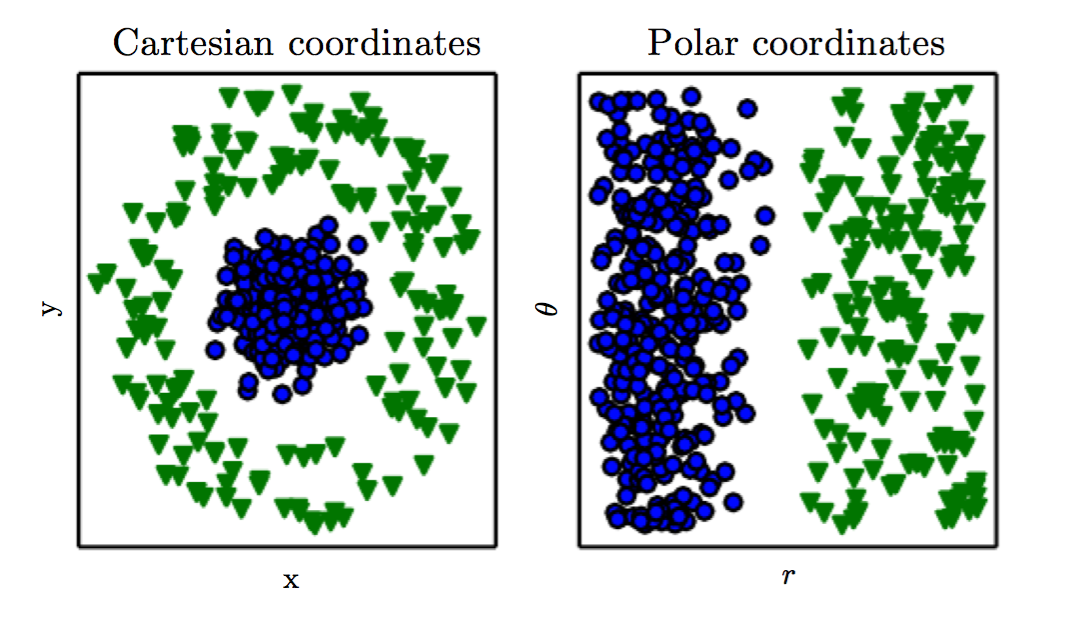
\includegraphics[width=4in]{fig/chap1/represent.png} 
   \caption{不同的表达形式的例子:假设我们要在如上散点图中画一条线分割两个不同种类的数据,左图是笛卡尔坐标系中的散点图,这个任务是不可能完成的。右图是该数据在极坐标系中的散点表示,这个任务可以通过画一条垂线就完成了。}
   \label{fig:represent}
\end{figure}

许多人工智能的任务可以通过手工设计合适的特征组并输入一个简单的机器学习模型来完成。比如,说话人的声道大小是说话人识别任务的一个有用的特征,他可以作为说话人是男人、女人或是小孩的一个强线索。


然而,对许多任务来说,我们很难去发现应该抽取什么样子的特征。比如,我们需要在一张照片中检测车辆。我们知道汽车有轮子,所以我们可能会把轮子作为汽车检测的一个特征。不幸的是,在像素的级别上描述轮子是非常困难的。轮子的几何形状非常简单,但是轮子上的阴影、金属部分的折射、保险杠的影响或前景物体的遮挡等让描述它变得非常复杂。


上述问题的一个解决方案是,我们不仅使用机器学习的算法去学习特征表达到输出结果之间的映射,也使用机器学习去学习起特征表达,这种方案被称为“表征学习”。表征学习通常可以获得比手工特征更好的表现,它也让AI系统在很少的人工干预下可以快速的适应新的任务。表征学习算法可以为一个简单的任务在数分钟之内找到一组好的特征,复杂的任务耗时则从几小时到几个月不等。为一个复杂的任务人工的设计特征需要耗费大量的时间和精力,甚至可能花费整个研究团队数十年的时间。


表征学习的一个经典算法叫做“自编码器”。自编码器有两部分组成:编码器把输入的数据转换到不同的表征空间;解码器把这个表征再转换回原始的数据。自编码器的训练目标一个是在不断的编码和解码的过程中保存尽量多的信息,另一个是在表征空间中有良好的属性。不同的任务需要自编码器有不同的属性。


不管是手工特征还是学习的特征,我们的目标通常是分离出观测数据的“变化因子”。在本文中,我们使用“因子”来表示不同的影响源,这些因子通常都不是通过乘法来组合的,这些因子也通常不能通过直接观测来量化。相反的,这些因子或许存在在物理世界中尚未发现的物体或力量中但对可观测的量造成了影响。这些因子也可能存在于人类大脑的结构中,提供对可观测数据的推理和抽象解释能力。当分析一段录音时,变化因子包括说话人的年龄、性别、口音和他所说的一字一句。当分析一幅汽车的图像时,变化因子包括车的位置、颜色、阳光的角度和亮度。


许多真实世界的AI应用面对的主要问题来源就是许多的变化因子影响着我们观测到的每一份数据。图像上一辆红色的车的像素值在夜晚的时候会非常靠近黑色。汽车的轮廓表现在不同的观测角度下是不同的。绝大多数的应用都需要我们对变化因子解耦并且丢弃那些我们不关心的变化因子。


从原始数据中抽取如上所说的高层次和抽象的特征固然是非常难的。如说话人口音在内的许多变化因子,都需要对数据具有非常精致和复杂、接近人类的理解能力才能获取。当获取一个合适的特征表达的难度几乎和解决原始问题相当的时候,表征学习似乎并不能给我们带来帮助。


“深度学习”通过表征的层级组合解决了表征学习中的核心问题。深度学习允许计算机通过学习一系列简单的概念来组成复杂的概念。图\ref{fig:deep_learning_intro} 展示了深度学习如何从图像中通过一些如边缘,角点,轮廓的简单的特征组合来表示一个人的。

\begin{figure}[htbp] %  figure placement: here, top, bottom, or page
   \centering
   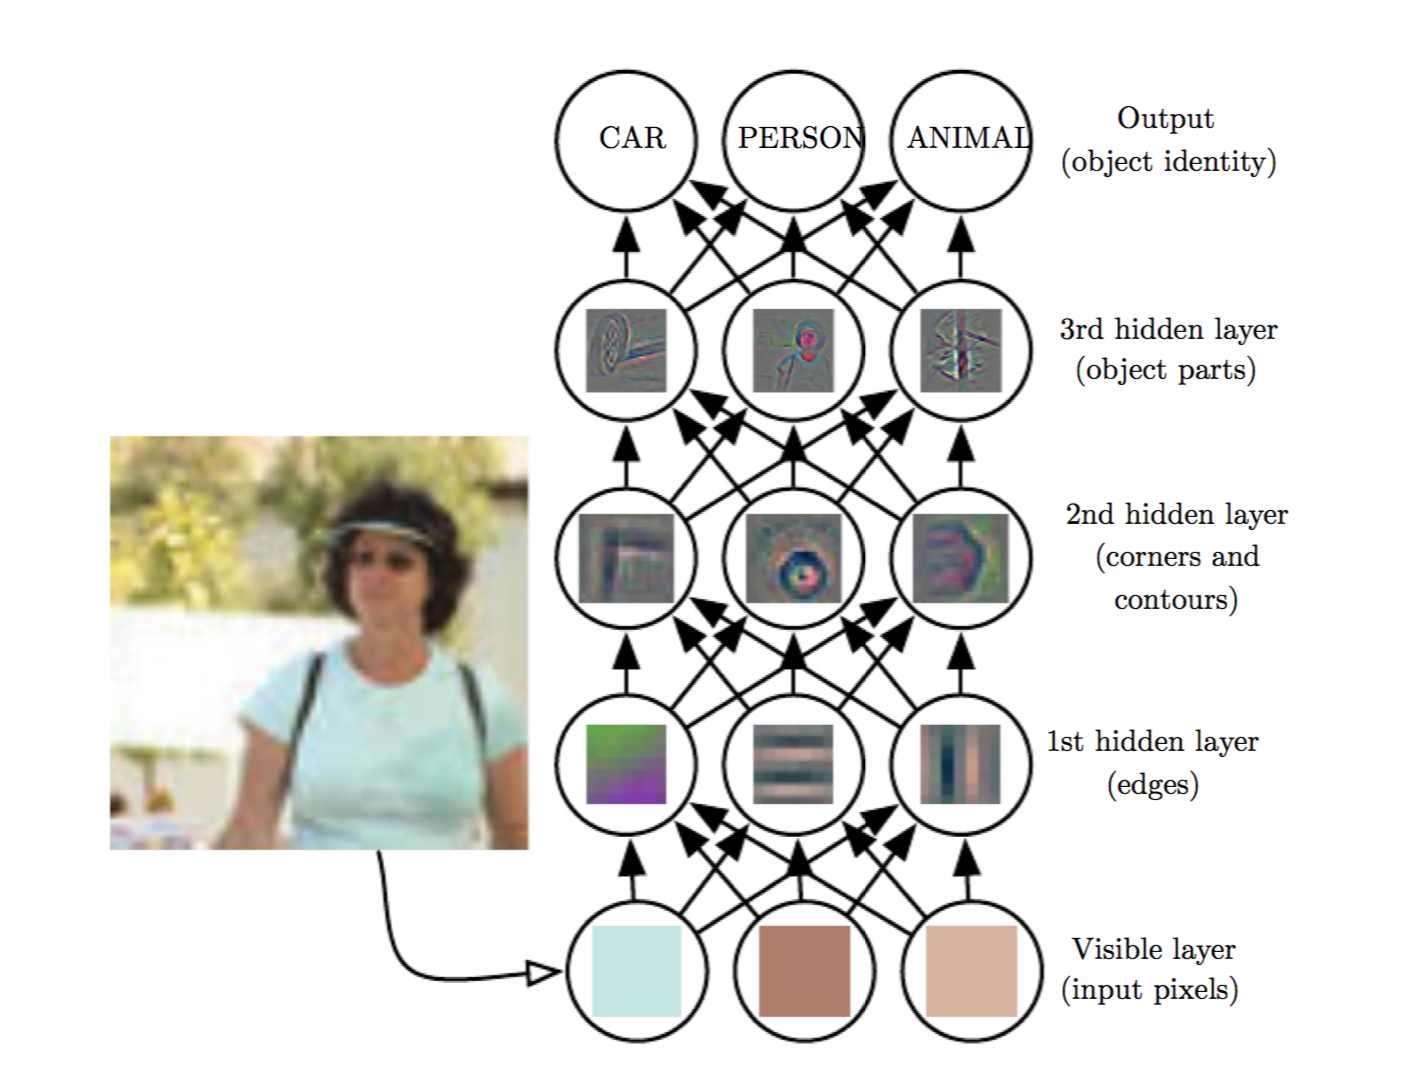
\includegraphics[width=5in]{fig/chap1/deep_learning_intro.png} 
   \caption{深度学习模型图解。对计算机而言,理解如像素值等的传感器捕获的原始数据是非常困难的。从一组像素值到物体标签的函数映射是十分复杂的,如果直接来学习或评估这个映射看起来是个不可能的。深度学习通过把这个复杂的映射分解成一系列的简单映射来解决这个问题,每个简单的映射是模型中一个不同的“层”(layer)。原始的数据输入被称为“可视层”,因为它包含着我们观察地到的变量。紧接着是一系列的“隐层”不断的从图像中抽取抽象的特征,这些层被称为“隐层”是因为他们的值不是由原始数据直接给出的,模型需要决定哪些概念对解释可观测数据之间的关联是有用的。图示为每个隐层所学习到的概念的可视化。第一个隐层可以十分容易的通过相邻像素之间的明暗对比抽取出边缘的信息,第二层则可以通过轮廓信息学习出角点和轮廓的信息,第三层则可以通过角点和轮廓的信息寻找到指定物体的一些部件信息。最终,通过对物体的部件描述,我们可以识别出图像中的物体。}
   \label{fig:deep_learning_intro}
\end{figure}


前馈神经网络或多层感知机(MLP)是深度学习的一个典型例子。多层感知机不过是把输入映射到输出的数学函数,而这个函数是由许多更简单的函数组成的,且我们可以认为应用不同的数学函数可以提供对输入数据的不同表征。


学习合适的表征是深度学习的一方面,另一方面是“深度”允许计算机学习到分步的计算过程。每一层的表征都可以被认为是计算机并行的执行了一系列的指令集后的记忆状态,更深层次的网络可以按照序列顺序执行更多的指令集。序列的指令拥有更强大的能力,因为它可以从前序的指令的结果中获得参考。根据深度学习的这些观点,并不是层中激活的所有信息都可以编码对解释输入数据的起作用的变化因子。表征会存储有利于算法执行、使得输入有意义的状态信息。在传统计算机程序中,状态信息可以类比于计数器或者指针,它与输入内容没有直接的关系,但是可以帮助深度学习模型组织其自身的处理过程。


有两种主要的方法可以测量一个模型的深度。第一种是统计在测试网络的过程中必须被执行的序列指令的数量,可以认为这是描述模型从输入到输出的流程图中的最长路径。就像相同的程序由于编程语言的不同会有不同的长度,对于同一个函数,其在流程图中的长度取决于我们把哪些步骤看作是独立的。图\ref{fig:flow_chart}描述了不同的语言是如何使得同一个结构拥有不同的深度。

\begin{figure}[htbp] %  figure placement: here, top, bottom, or page
   \centering
   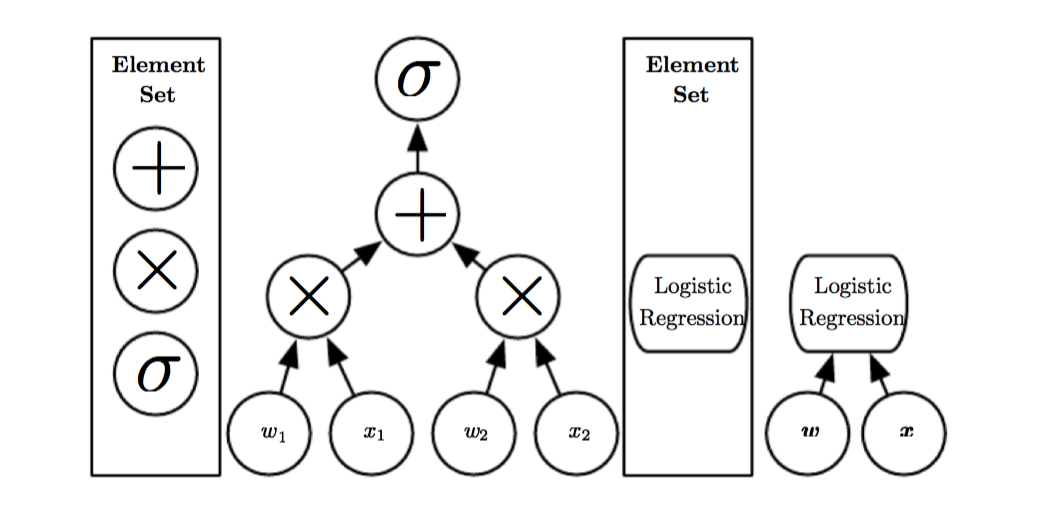
\includegraphics[width=5in]{fig/chap1/flow_chart.png} 
   \caption{每一个节点表示一个不同的操作,图示为从输入到输出映射的计算图。深度是从输入到输出的最长路径,但它的计算依赖于对独立计算步骤的定义。上图描述的是逻辑回归的模型$\delta(w^Tx)$,$\delta$是逻辑回归的sigmoid函数。如果我们认为加法、乘法和sigmoid操作是计算机语言的元素级操作,那这个模型的深度就是3;如果我们认为逻辑回归本身就是就是元素级操作,那这个模型的深度就是1。}
   \label{fig:flow_chart}
\end{figure}


另一个由深度概率模型所使用的概念是,深度并不是计算流程图的深度,而是描述概念之间的层级结构的组织图的深度。在这个概念中,由计算流程图得到的深度往往比概念组织图得到的深度要深得多。比如,一个AI系统如果在观测一副有一只眼睛在阴影中的人脸图像时可能刚开始只能观测到一只眼睛,等到能发现整个人脸的时候,AI可能会推理出另一只眼睛也是存在的。在这个例子中,概念组织图只有两层:一层是检测眼睛,一层是认知人脸;但如果我们n次调优每一层概念时,计算流程图中则有2n层。


该选择计算流程图还是概念组织图来计算深度是没有定论,而且每个人选择构建图所使用的最小元素也不尽相同,因此对一个架构来说并没有一个唯一的正确深度,就像对计算机程序来说也没有一个唯一的正确深度。同样,对于一个模型来说,多深才叫“深”也没有定论。可以肯定的是,相比传统的机器学习来说,深度学习可被认为是一种含有大量计算的函数学习和概念学习的模型。

总之,本书的主题“深度学习”是AI的一种实现方法,而且它也是一种可以使得机器自身通过数据和经验不断提升的机器学习方法。本书的作者们认为,深度学习是构建在真实世界处理复杂问题的AI系统的目前唯一可行的方法。深度学习是机器学习中很强大很灵活的一种方法,因为它学习的是如何将真实环境中的任务以嵌套的层级概念表达出来,通过这些嵌套的概念,它可以将底层的表征不断抽象为含有语义的更高层的特征。图\ref{fig:ai_approach}显示了不同的AI方法之间的关联,图\ref{fig:ai_discipline}概括了这些方法是如何实现的。

\begin{figure}[htbp] %  figure placement: here, top, bottom, or page
   \centering
   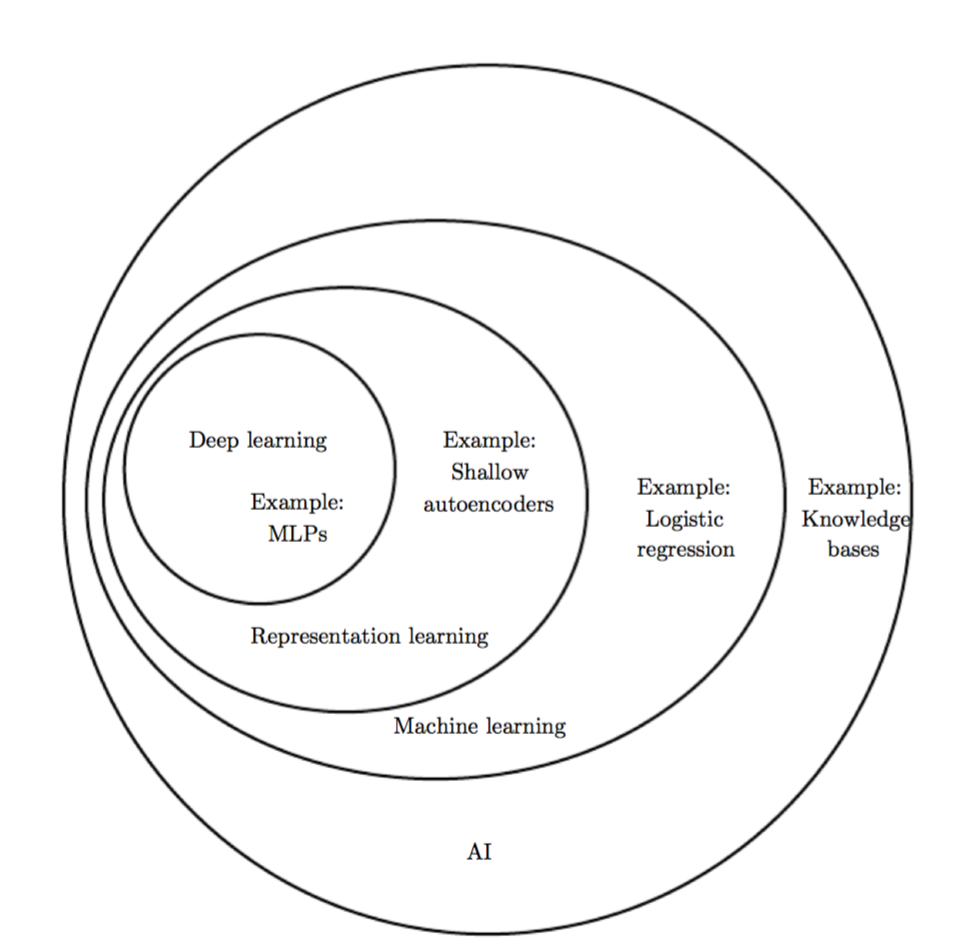
\includegraphics[width=6in]{fig/chap1/ai_approach.png} 
   \caption{这个维恩图解释了为什么深度学习也是一种表征学习的方法和机器学习方法。维恩图的每个部分都给出了一个AI方法的实例。}
   \label{fig:ai_approach}
\end{figure}

\begin{figure}[htbp] %  figure placement: here, top, bottom, or page
   \centering
   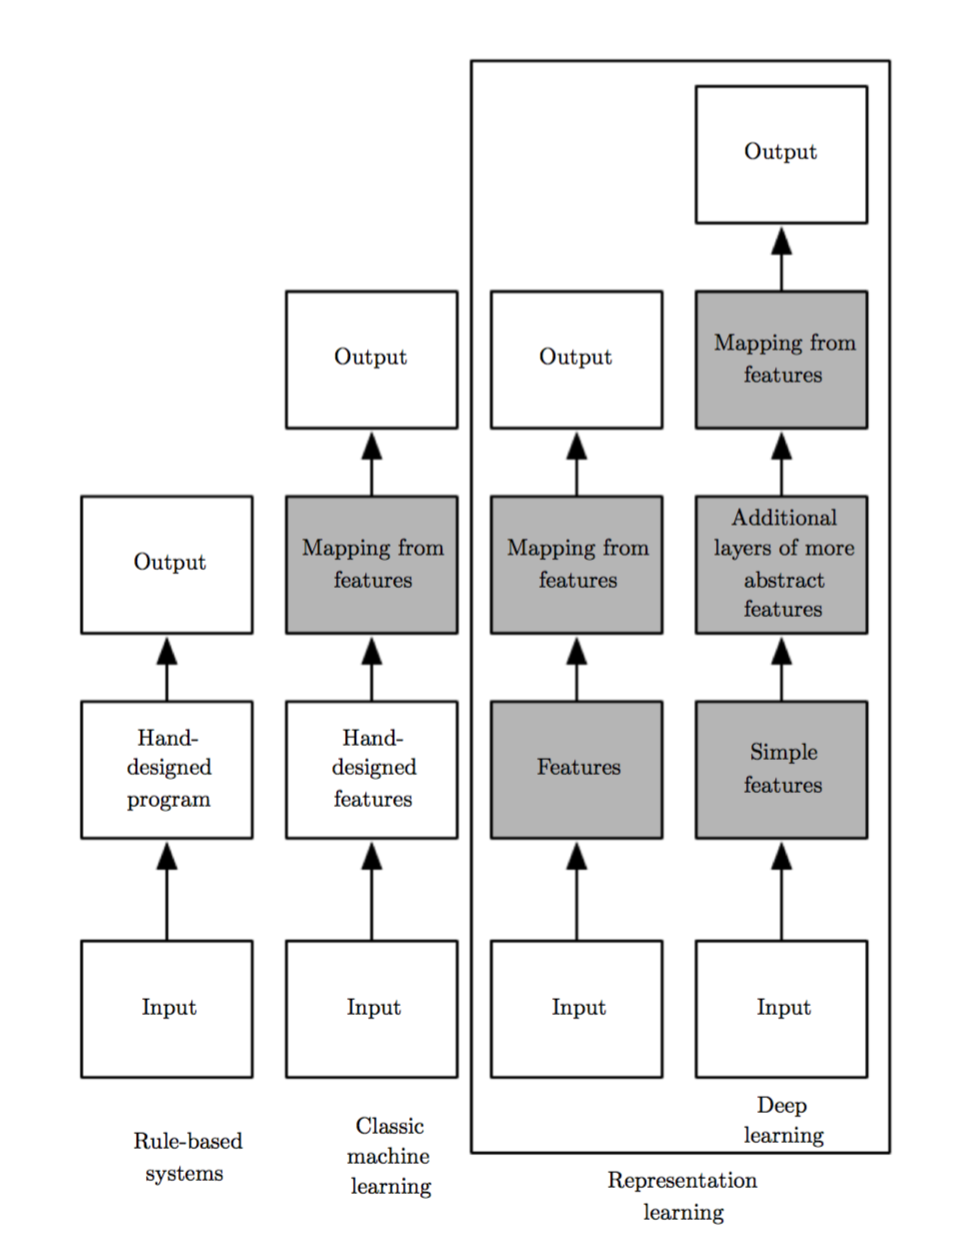
\includegraphics[width=4in]{fig/chap1/ai_discipline.png} 
   \caption{此图显示了不同的AI算法是如何组成AI系统的不同部分的。深色的框表示这个模块是可以从数据中学习的。}
   \label{fig:ai_discipline}
\end{figure}

\section{谁应该读这本书}

这本书对很多类型的读者都有用处,但我们主要为两类读者而写。一类是正在学习机器学习的本科生或研究生,或准备开始在深度学习和人工智能的研究领域大展身手的人。另一种是想要快速把深度学习技术应用在他们的产品中,但没有机器学习或统计背景的工程师。深度学习已经在多个软件领域中获得了成功,包括计算机视觉、语音识别、自然语言处理、机器人、生物信息学和化学、视频游戏、搜索引擎、在线广告及金融等。


为适应尽可能多的读者,本书主要由三部分构成。第\ref{part:1}部分介绍基础的数学工具和机器学习的概念。第\ref{part:2}部分介绍了最为广泛使用的深度学习算法。第\ref{part:3}部分介绍了被认为对深度学习的进一步研究十分重要的更又去的想法。


读者可以根据自身的背景或感兴趣的方向自由的阅读本书。对线性代数、概率和基础机器学习算法熟悉的读者可以跳过第\ref{part:1}部分,而只想实现一个可用的深度学习系统的读第\ref{part:2}部分就够了。图\ref{fig:1.6}提供了本书的一个高层的组织流程图。


我们写本书的时候假设本书的读者都具有计算机科学的相关背景,因此我们也认为大家都熟悉编程、对计算性能和算法复杂度有基本认识、有入门级的微积分和图论的知识。

\begin{figure}[htbp] %  figure placement: here, top, bottom, or page
   \centering
   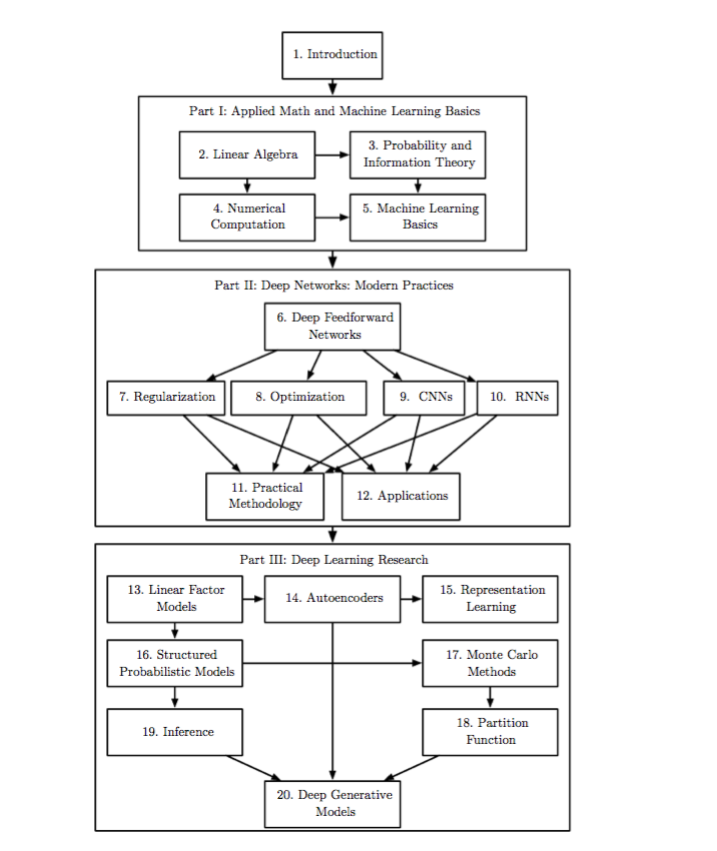
\includegraphics[width=7in]{fig/chap1/1.6.png} 
   \caption{本书的组织图。如果箭头从第A章指向第B章,意味着理解章节B的需要A的知识。}
   \label{fig:1.6}
\end{figure}


\section{深度学习历史趋势}
伴随着历史的轨迹来看深度学习是最荣易让人理解的一种方式。我们找出了一些深度学习发展的关键趋势而非提供一个详尽的发展历史:

\begin{itemize}
\item 深度学习有着悠长和丰富的历史,也有许多人抱持着不同的哲学观点,但它的发展并非一帆风顺。
\item 当可以获取的训练数据逐步增长时,深度学习的成效也在增长。
\item 当适用于深度学习的软硬件提升时,深度学习模型的大小也在增长。
\item 深度学习解决复杂问题能力和精确度随着时间不断提升。
\end{itemize}

\subsection{改变神经网络命运的人们}
我们期待着本书的读者听说过深度学习这个令人兴奋的新技术,能非常惊喜的看到有一本书在介绍这个新兴领域的历史。事实上,深度学习在1940年左右就已经出现。深度学习显得很新是过了很多年前它并不十分流行,而且它有许多不同的名字,直到最近才被称为深度学习。深度学习被多次更名,这也可以反映出不同的研究人员和不同的角度观点带来的影响。


本书并不意在介绍深度学习的全面历史,但是一些基础的认知可以帮助我们理解深度学习。广泛的说,深度学习的发展有三次浪潮:深度学习在1940-1960年间被认为是“控制论”,在1980-1990年间被称为“联结学”,从2006年后才被称为深度学习。这在图\ref{fig:1.7}中量化的表示了。


一些早期的学习算法在今天我们认识到其实是生物学习的计算机模型,即模仿大脑学习的机制。因此,深度学习的一个别名就是人工神经网络(ANNs),与之一致的观点是深度学习模型是受生物大脑启发的一个工程系统(人类大脑或其他动物的大脑)。这种机器学习中使用的神经网络有时候也会被用来理解大脑运行的机制,但这些网络一般没有被设计成实现生物机理的真实模型。从神经角度看深度学习的观点主要有两个思想。一个是大脑证明了智能的行为是可能的,一个直观的想法就是发现大脑运行背后的计算规则并复制其能力。另一种观点是,理解大脑和人智力背后隐含的原理是非常令人感兴趣的,所以揭示了这些基础科学问题的机器学习模型除了解决工程应用的问题外也是非常有意义的。


现代所说的深度学习已经超越了神经角度描述的任何种类的机器学习模型,它成为了一种更为普世的学习多层结构的指导原则,可以被应用于非神经学启发的机器学习模型构建。

\begin{figure}[htbp] %  figure placement: here, top, bottom, or page
   \centering
   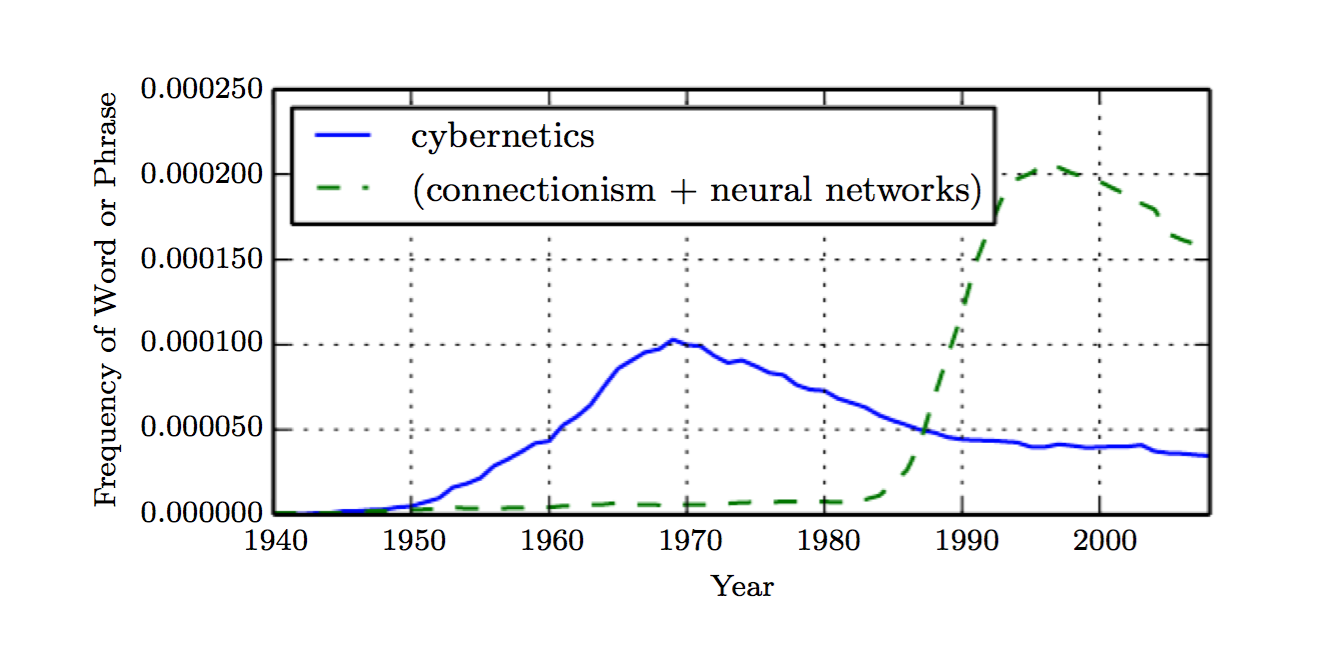
\includegraphics[width=4in]{fig/chap1/1.7.png} 
   \caption{本图展示了人工神经网络研究的发展史上三次浪潮中的两次,根据Google Books 中提到控制论、联结学或神经网络的批量得出的测量(第三次浪潮是最近才出现的)。第一次浪潮是在1940-1960间出现的控制论,伴随着生物学习理论的发展和第一个允许训练的单个神经元的感知元模型的建立。第二次浪潮是1980-1995年出现的联结学,那时出现了反向传播算法,我们可以训练拥有一到两个隐层的神经网络了。现在是第三次浪潮,从2006年开始的深度学习,直到2016年才被写进书中。不过另外两次浪潮也一样,也是滞后于相关科技的发展很长时间才被书中收录。}
   \label{fig:1.7}
\end{figure}


现代深度学习的先驱是受神经学启发的简单线性模型。这类模型有$n$个输入$x_1,...,x_n$和一个输出$y$,目标是学习一组权重$w_1,...,w_n$使得$f(\textbf{x},\textbf{w}) =x_1w_1+...+x_nw_n$。第一次神经网络研究的热潮如图\ref{fig:1.7}所示,被称为控制学。

McMculloch-Pitts神经元是一个描述大脑功能的早期模型,这个线性模型可以通过$f(\textbf{x},\textbf{w})$输出的正负来做二分类,当然,权值需要根据分类任务的不同进行相应的调整,而这些权值是需要人工设置的。直到1950年代,感知机出现了,它是第一个可以根据不同类别的数据对权值进行自动调整的模型。与此同时出现的自适应线性元件(ADALINE),通过简单地返回函数$f(\textbf{x})$来预测一个实数,也具有从数据中学习预测数字的能力。

这些简单的学习算法极大的影响了现代机器学习算法的版图。用于训练ADALINE的算法叫做随机梯度下降,经过稍微修改的随机梯度下降算法是目前绝对主流的深度学习训练算法。


感知机和ADALINE使用的$f(\textbf{x},\textbf{w})$类型的模型被称为线性模型。这类模型至今仍然被广泛的使用着,但如今的训练方法很多时候和最初的训练方法不同。


线性模型有许多局限性。最著名的一个是他不能学习异或函数,即$f([0,1],\textbf{w}) =1$ 且$f([1,0],\textbf{w}) =1$,但$f([0,0],\textbf{w}) =0$且$f([1,1],\textbf{w}) =0$。发现了线性模型这一缺陷的批评家引起了普遍性对生物启发学习的反弹,引起了第一次神经网络热度的退潮。


现在,神经科学仍然被认为是深度学习的一个重要灵感来源,但它已经不再被认为是这个领域的绝对指南。


今天,神经科学对深度学习研究的影响逐渐减弱,因为我们没有足够关于大脑运作机制的信息可以给出指导。如果要深刻理解大脑使用的算法,那就必须同时观测成千上万互相连接的神经元的活动,然而我们做不到这些。因此,我们和理解最简单和被研究的最透彻的大脑部分都相距甚远。


神经科学使得我们希望用一个深度学习的模型来解决不同的问题。神经学家发现雪貂可以利用大脑的声音处理区域学会“看”,如果这个区域被输入视觉信号的话。这证明了多数哺乳动物也许是使用某种单一的算法来使得大脑解决不同的问题。在这个假设出来之前,机器学习的领域是碎片化的,来自不同社区的研究人员在研究不同的领域,如自然语言处理、计算机视觉、运动规划和语音识别等。如今,这些社区仍然是独立的,但深度学习的研究团队可能会同时研究上面所说的许多领域。


我们可以从神经科学中得到一些粗略的指导。如通过不同计算单元的联结来使得系统变得智能就是受到大脑的启发。Neocognitron创造的一种处理图像的强大模型框架的灵感就来自于哺乳动物的视觉系统,随后这个模型成为了现代卷积网络的基础框架,这个模型在第章会再详细介绍。目前所使用的神经网络绝大多数建立在一个叫做\emph{线性整流单元}的模型基础上, Cognitron提供了一个更复杂的模型,这个模型也是受到大脑运作机制的启发而来。现代这个简化版本是由许多的观点整合而来的,如Nair、Hinton、Glorot就援引了神经科学的观点,Jarrett就更多的从工程角度进行了援引。神经科学虽然是一个重要的灵感源泉,但它不需要被视为刚性的指导。我们知道真实的神经元与线性整流单元的运算机制不尽相同,但更为写实的神经元工作机制并没有给机器学习带来很大的提升。虽然神经科学成功的激发了一些神经网络\textbf{结构}的建立,但我们现在对神经元的学习机制的掌握还不够,还不足以为训练这些结构的\textbf{学习算法}带来足够的指引。


媒体经常强调深度学习和大脑有多么相似。虽然深度学习的研究者和其他机器学习领域的研究者相比更容易引用脑科学的文章,但我们不应该把深度学习看做对大脑的一种模拟。现代深度学习从许多领域汲取养分,特别是一些应用数学的领域,如线性代数、概率论、信息论以及数值优化等。当一些深度学习研究人员援引神经科学作为一种重要灵感源泉时,另一些研究人员或许压根不关心神经科学。


理解大脑在算法级别的运作的工作是值得关注的。这类工作被称为是“计算神经科学”,是不同于深度学习的一个研究领域,许多研究者会在这两个领域之间游走。深度学习的领域主要关心的是如何建立具有可解决问题的智能系统,而计算神经科学的领域的重点工作是建立大脑运作的更精确的模型。


在1980年代,迎来了神经网络研究的第二次热潮,这次热潮主要是通过\emph{联结学}或\emph{并行分布式处理}的运动产生。联结学在认知科学中产生,认知科学是一种为了理解大脑的跨学科研究,并且有许多不同的层面的分析。在1980年代早期,许多认知科学家都在研究符号推理,尽管符号推理很流行,但是符号模型是如何用神经元在大脑中实现的都难以解释。联结学家就开始研究那些可以被神经元实现的认知模型,复兴了心理学家Donald Hebb在1940年代提出的许多想法。


联结学的核心思想就是通过联结许多简单的计算单元可以实现智能。这个洞见也适用于生物神经系统的神经元和计算模型的一些隐藏单元。


1980年代联结学运动中产生了一些核心观念对今天的深度学习来说仍然至关重要。


其中一条概念就是\emph{分布式表达}。这个概念描述的是每个对系统的输入都应该由许多的特征来表达,而每个特征都应该参与到许多的输入的表达。比如,我们有一个可以识别汽车、卡车、鸟的视觉系统,我们识别的物体可能是红的、绿的或者蓝色的。一种表达这些输入的方式是,我们有许多独立的神经元组或隐藏神经元组来处理九种不同的排列组合:红卡车、红汽车、红鸟、绿卡车、绿汽车等。这需要九个不同的神经元组,而且每一组都需要独立的学习相关的物体和颜色的概念。一个提升效能的方法就是使用分布是表达,使用三组神经元描述颜色,三组神经元描述物体信息,这样就只需要六组神经元而非九组。学习红色的神经元可以从汽车、卡车和鸟的图像中学习,而不限于特定的类型。分布式表达对本书非常重要,会在第\ref{chap:15}章进行更详细的描述。


另一个联结学运动的主要成就是成功的运用了反向传播来训练深度神经网络,并使得反向传播算法流行起来。这个算法在历史的流行度上有过跌宕起伏,但在目前深度学习的领域占了绝对的主导地位。

在1990年代,研究者们在使用神经网络进行序列模拟方面取得了很大的进步。Hochreitrt和Bengio解决了建模长序列的几个关键数学难题,在第\ref{sec:10.7}中会提到。Hochreiter和Schmidhuber提出了长短期记忆网络(LSTM网络)来解决序列建模中遇到的一些难题。如今,LSTM广泛的应用在很多序列建模的任务中,比如Google就使用它来做一些自然语言处理的工作。


神经网络的第二次浪潮一直持续到二十世纪九十年代中期。风险投资公司在寻求基于神经网络的和其他AI技术的投资机会时,往往会提出十分具有野心但不切合实际的要求。当AI的研究不能满足这些不合理的期望时,投资者会感到失望。而与此同时,机器学习的其他领域取得了进步。核方法和图模型在许多重要任务上都获得了良好的表现。这两个因素导致了神经网络浪潮的一次衰退,这次衰退延续到了2007年。


在这次退热中,神经网络还持续的在一些任务上取得进展。加拿大先进技术研究院(CIFAR)通过倡议进行神经计算和自适应感知(NCAP)的研究保持了神经网络研究的存续。这个项目团结了以多伦多大学的Geoffrey Hinton、蒙特利尔大学的Yoshua Bengio和纽约大学Yann LeCun为首的机器学习研究团队。CIFAR NCAP研究计划具有多学科的自然属性,有神经科学家、人类专家以及计算机视觉的专家参与其中。


在那个时候,深度网络被普遍的认为是难以被训练的。我们现在知道了二十世纪八十年代就存在的算法就可以工作的非常好,但在2006年前我们还没清楚的认识到这一点,这个原因可能是那些算法的计算量对当时的硬件来说太大了,难以进行很多次实验。


神经网络的第三次热潮由2006年的一次突破开启。Geoffrey Hintion展示了一种叫做深度信念网络的神经网络结构,这个网络可以用贪婪的逐层预训练策略来达到高效的训练,这个网络在\ref{sec:15.1}中会展开详细的介绍。CIFAR附属的其他研究团队很快的就发现了这个策略也可以适用于训练其他的深度网络,并可以系统的提高在测试样本中的泛化能力。这次热浪推动了\emph{深度学习}的普及,研究者们现在能训练以前难以想象的更深的神经网络, 并且开始重点关注深度的理论意义。现在,深度神经网络已经超越了其他机器学习技术的AI系统,也超过了使用手工特征的智能系统。第三次浪潮在本书撰写的时候仍然在持续,虽然在这次浪潮中深度学习研究的重点发生了极大的变化。第三次浪潮始于对新的无监督学习技术和在小数据集上获得良好泛化能力的深度模型的关注,但现在的人们对于更老的有监督学习算法以及处理大量标注数据集的深度模型的能力更感兴趣。


\subsection{不断变大的数据集}
\label{sec:1.2.2}


可能很多人会疑惑,第一次对人工神经网络的实验是在二十世纪五十年代,但为什么深度学习直到最近才被认为是一项关键技术。在二十世纪九十年代的时候,深度学习就在商业应用中取得了成功,但那时深度学习更被认为是一项只有专家能够使用的艺术而非技术,不过深度学习算法确实是需要一些技巧才能获得良好的表现。幸运的是,随着训练数据的不断增大,所需要的技巧也不断减少。今天在复杂任务上获得与人类水平相当的学习算法和二十世纪八十年代难以解决的玩具问题\footnote{指不是需要实际解决,但可以用来帮助更复杂问题寻找答案的问题}所使用的学习算法基本是相似的,但训练模型的算法简化了,可以训练非常深的结构。最重要的进步是如今我们可以给算法提供所需要的资源,帮助算法取得成功。图\ref{fig:1.8}展示了数据集的大小是如何与日俱增的。这种趋势是被整个社会的数字化所驱动,当计算机领域的活动越来越多,越来越多的行为也被记录。随着电脑互联的程度增加,集中这些记录变得更加容易,也更加容易的把这些数据变为适用于机器学习应用的数据集。“大数据”时代使得机器学习更加容易,因为统计估计这个关键负担被认为是减轻了不少,因为模型对少量数据观测后在新的数据上也能获得不错的泛化能力。到2016年,一个粗略的规则是5000个标注的数据可以获得可接受的表现,到标注数据达到千万级别时模型的能力能与人相比或超越人。当训练数据少于此的时候如何让模型仍然获得成功是一个重要研究领域,特别侧重于如何用无监督或者半监督的算法使用大量的未标注数据。

\begin{figure}[htbp] %  figure placement: here, top, bottom, or page
   \centering
   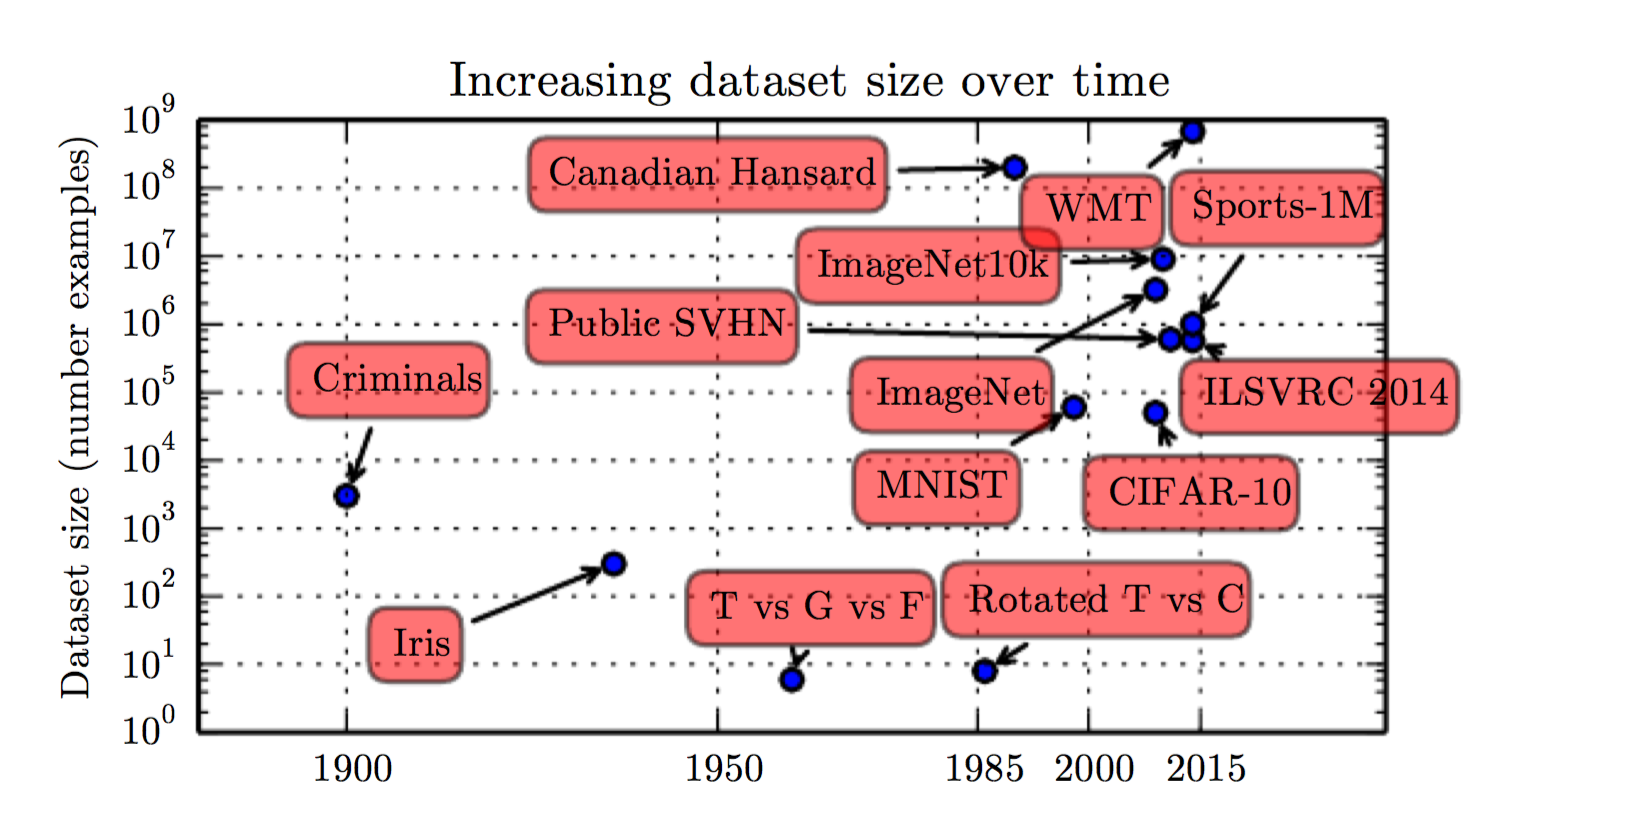
\includegraphics[width=5in]{fig/chap1/1.8.png} 
   \caption{数据集随着时间剧增。在二十世纪初期,统计学家使用成百上千次的手工编译研究数据集。在二十世纪五十年代到八十年代期间,受生物学启发的机器学习先驱经常使用的是小的、合成的数据集,比如信件的低分辨率位图,这些数据的使用是为了减少计算量的基础上使用神经网络实现特定功能。在二十世纪八十年代到九十年代,机器学习变得更加偏统计,并且开始使用万量级的数据集,比如MNIST(如\ref{fig:1.9})就是手写数字的扫描。在二十一世纪的前十年,出现了更多更复杂的数据集也是在这个量级,比如CIFAR-10就在持续的增加。在二十一世纪一零年代的前半部分,从十万到千万量级的更大的数据集完全的改变了深度学习能力的界限。这些数据集包括Street View House Numbers,不同版本的ImageNet,Sports-1M等。在图的顶端我们可以看到翻译句子的数据集,比如由Canadian Hansard构造的IBM数据集,还有WMT2014英法翻译数据集等都远超了其他数据集的量级。}
   \label{fig:1.8}
\end{figure}


\begin{figure}[htbp] %  figure placement: here, top, bottom, or page
   \centering
   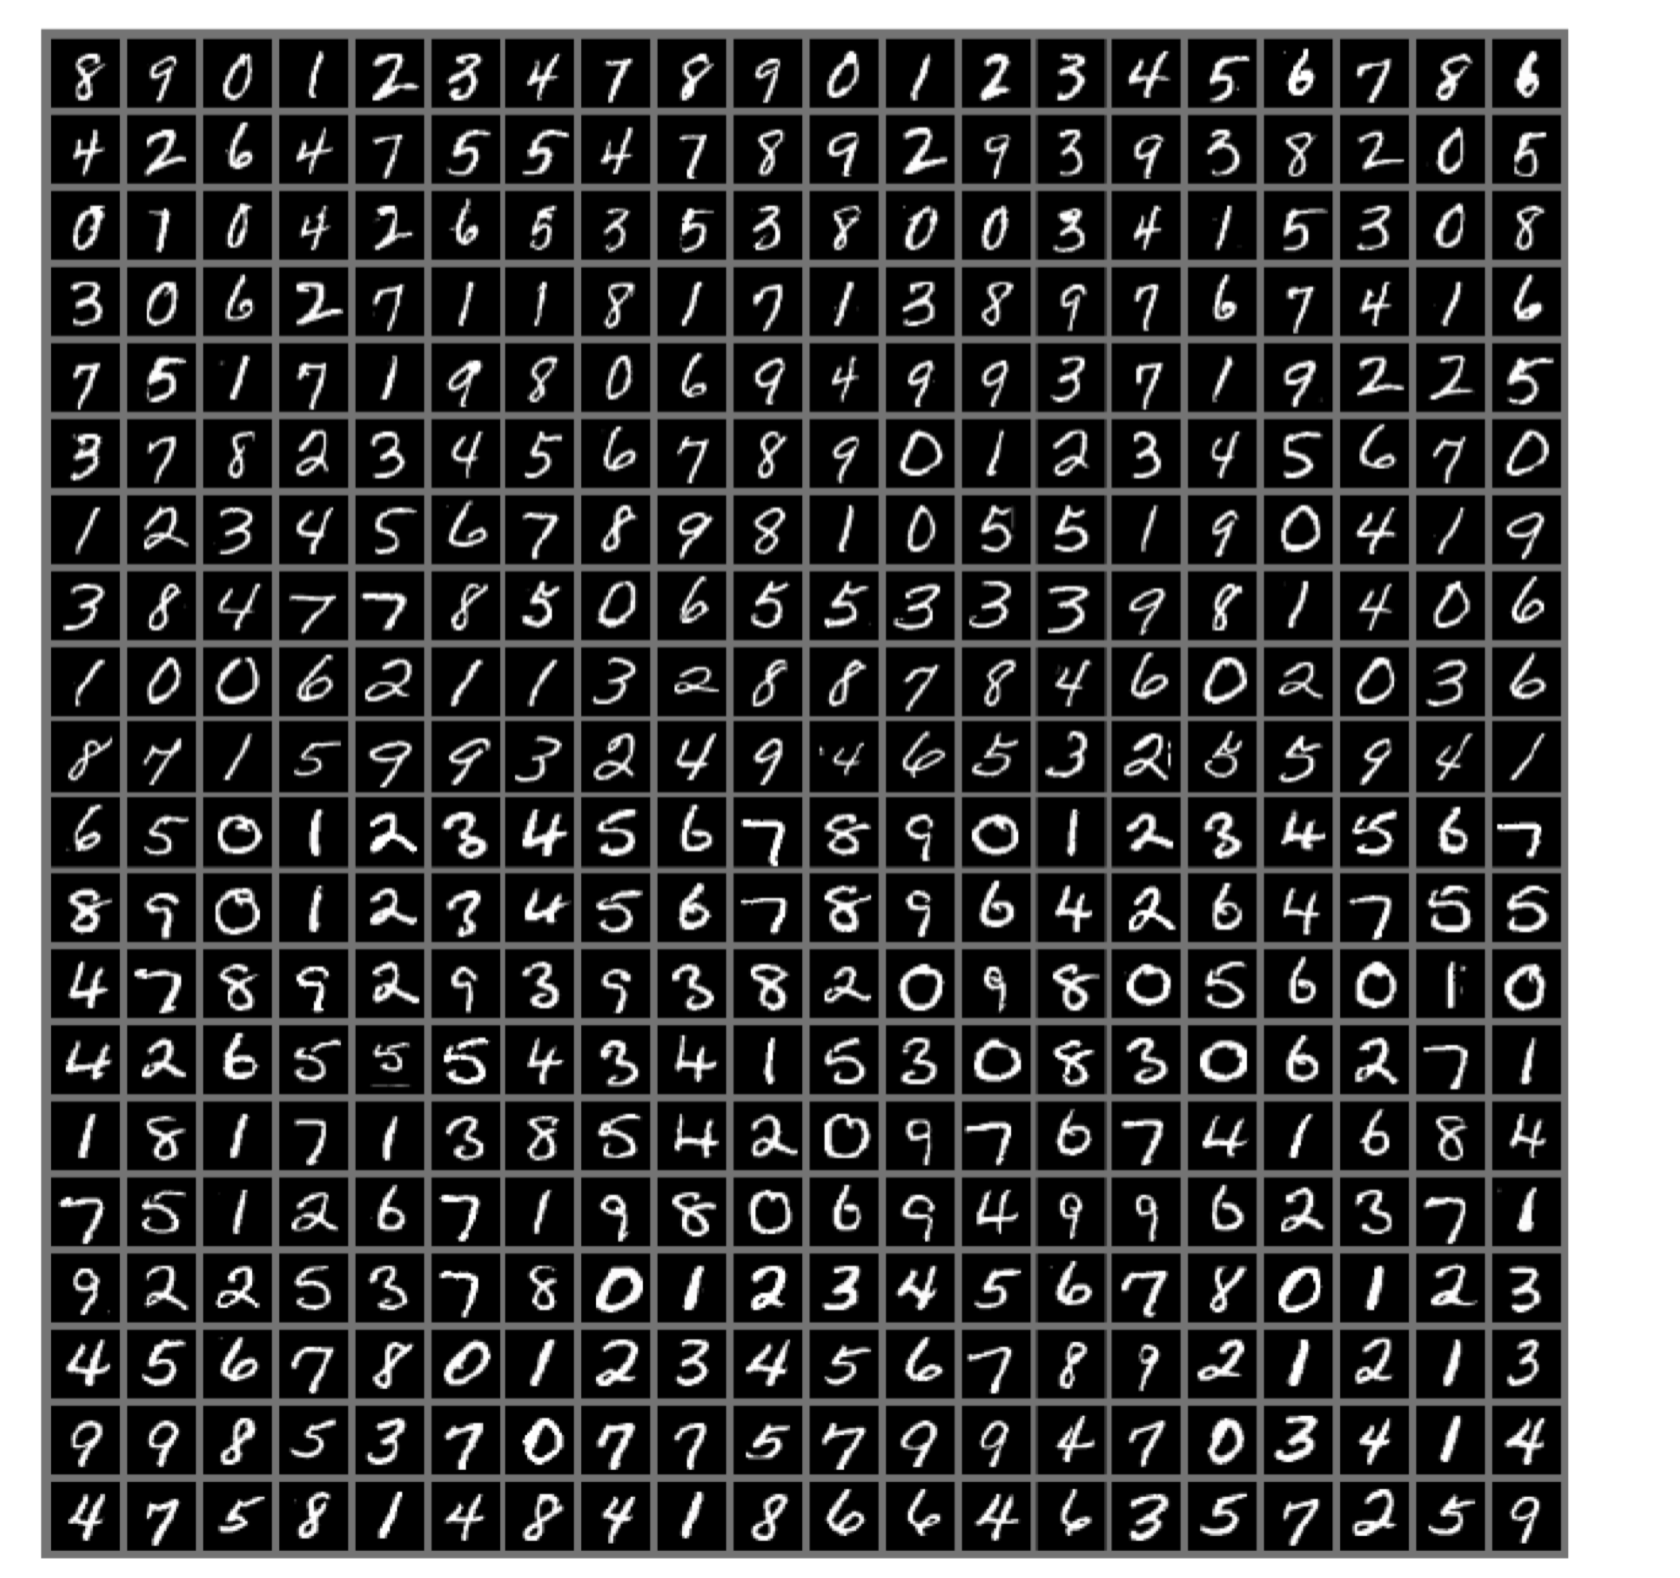
\includegraphics[width=4in]{fig/chap1/1.9.png} 
   \caption{MNIST数据集的示例。“NIST”意思是国家标准技术研究所,就是一开始收集这些数据的机构。“M”意思是“改变的”,因为这批数据为了使得机器学习算法更简单的应用进行了预处理。MNIST数据集中有0-9的手写数字的扫描数据以及相应的标签。这个简单的分类是深度学习研究中最简单也最为广泛使用的测试。尽管这个任务对现代的技术来说很简单,但仍然很流行。Geoffrey Hinton称其为“机器学习的果蝇”,意味着机器学习研究者可以在可控的实验条件下研究他们的算法,正如生物学家经常使用果蝇来帮助研究一样。}
   \label{fig:1.9}
 \end{figure}
   

\subsection{不断变大的模型}
\label{sec:1.2.3}
另一个神经网络现在获得广泛成功的原因是如今我们有计算资源可以计算更大的模型。联结学的主要认知之一就是当有许多的神经元联结在一起的时候动物才能变得智能。一个独立的神经元或者一小组神经元并不是特别有用。


生物的神经元并不总是密集的联结的。如图\ref{fig:1.10},我们的机器学习模型中每个神经元都有一定的连接数,这个数量随着时间变化已经逼近了哺乳动物大脑的连接数的量级。


就神经元的总数而言,神经网络在今天之前的量级小的令人惊讶。




\part{应用数学与机器学习基础}
\label{part:1}

本部分介绍一些用于理解深度学习的基础数学概念。我们从定义函数和一些变量的应用数学开始,然后找到这些函数的最高点和最低点并量化置信度。


接着,我们会介绍机器学习的基本目标,并介绍如何使用特定的模型来模拟表示并完成这些目标。比如设计一个损失函数来描述模拟值和真值的差距,并使用训练算法来最小化损失函数。


这个基本的框架是许多机器学习算法的基础,包括一些不那么深的机器学习模型都有用到。在本书后续部分,我们会使用这个框架来建立深度学习算法。

\chapter{线性代数}
\label{chap:2}
%%%%%%%%%%%%%%%%%%%%%%%%%%%%%%%%%%%%%%%%%%%%%%%%%%%%%%%%%
%%%%%%%%%%% author:pascal_meng@outlook.com %%%%%%%%%%%%%%
%%%%%%%%%%%%%%%%%%%%%%%%%%%%%%%%%%%%%%%%%%%%%%%%%%%%%%%%%

\section{标量、向量、矩阵和张量}
\label{sec:2.1}

\section{矩阵和向量乘法}
\label{sec:2.2}

\section{单位矩阵和逆矩阵}
\label{sec:2.3}

\section{线性相关和和线性空间}
\label{sec:2.4}

\section{秩}
\label{sec:2.5}

\section{特殊的矩阵和向量}
\label{sec:2.6}

\section{特征分解}
\label{sec:2.7}

\section{奇异值分解}
\label{sec:2.8}

\section{摩尔-彭若斯广义逆}
\label{sec:2.9}

\section{求迹}
\label{sec:2.10}

\section{行列式}
\label{sec:2.11}

\section{示例:主成分分析}
\label{sec:2.12}
%%%%%%%%%%%%%%%%%%%%%%%%%%%%%%%%%%%%%%%%%%%%%%%%%%%%%%%%%
%%%%%%%%%%%%%%% author:wulemilly、msnh %%%%%%%%%%%%%%%%%%
%%%%%%%%%%%%%%%%%%%%%%%%%%%%%%%%%%%%%%%%%%%%%%%%%%%%%%%%%


\documentclass{article}
\usepackage{CJK}
\usepackage{amsmath}
\usepackage{graphicx}
\usepackage{amssymb}
\begin{CJK*}{GBK}{song}
  \title{第三章    概率论与信息论}
\begin{document}
  \maketitle
  \paragraph{}
  在这一章节,我们介绍概率论与信息论。
  \paragraph{}
  概率论是一个表示不确定性现象的数学框架。它将不确定性问题进行量化并为得到新的不确定性结论做出了公式推导。在人工智能应用领域,我们运用了概率论的两种主要方法。首先,概率法则告诉我们如何解决AI (人工智能)领域的问题,因此我们利用概率论设计相关算法来计算或运用多种表达式来近似解决该问题。其次,我们可以利用概率论和信息论从理论上来分析人工智能系统的行为。
 \paragraph{}
  概率论是科学与工程多学科交叉的一种基本工具。我们提供本章主要为致力于软件工程领域的读者提供相关的概率论知识,以确保读者可以理解本书的内容。
  \paragraph{}
  概率论为我们提供不确定性的思想并解释不确定性的原因,信息论使我们能够量化一个不确定性的概率分布。
  \paragraph{}
  如果您已经熟悉概率论与信息论,您可能希望跳过这一章,但是3.14节是我们需要关注的重点,它描述了我们用来描述机器学习的结构化概率模型的图表。如果您对这些科目没有深入的研究,本章将为您高效顺利开展深度学习项目的研究提供帮助,但是除此之外我们还是推荐您去阅读其他的相关内容	,比如Jaynes(2003)。

   %--section 1--%

  \section*{3.1 什么是概率论?}
    \paragraph{}
    计算机科学的许多分支主要是处理那些完全是确定性的实体。程序员通常可以安全地假定CPU可以完美无瑕的执行每条机器指令。在硬件中的错误确实发生,但是它还不足以在设计大多数软件应用程序的时候考虑它的影响。由于许多计算机科学家和软件工程师一般是处理比较确定性的问题,但是机器学习中大量使用概率论知识可能会令他们感到吃惊。
    \paragraph{}
    这是因为机器学习必须处理不确定的数据,有时也可能需要处理的随机数(不确定的),不确定性和随机性的产生来源于很多方面。从20 世纪80年代以来,研究人员已经为使用概率论来量化不确定性因素提供了非常可信的论据,这里提出的许多总结性的结论或启发参看Pearl (1988)。
    \paragraph{}
    许多事情都需要去推理它们存在的不确定性。事实上,除了数学可以通过定义来确定其真实性之外,很难保证任何一个绝对真实的命题,或任何一个绝对的事件都会发生。
    \paragraph{}以下是3种不确定性因素的来源:
    \subparagraph{}
    1.	在系统形成之时就存在固有的随机性。例如,在量子力学领域,亚原子的运动学都是用概率来描述的。我们也可以想象一个场景,我们假定一个动态随机的一个场景。比如一种卡牌游戏,所有的卡牌都是按照随机顺序排列的。
     \subparagraph{}
     2.	不完全的可观测性。当我们无法观测到所有的变量是如何驱动这个系统的时候,即便是个确定的系统也存在不确定性。例如一个蒙提霍尔问题。 你参加电视台的一个抽奖节目。台上有三个门,一个后边有汽车,其余后边是山羊。主持人让你任意选择其一。然后他打开其余两个门中的一个,你看到是山羊。这时,他给你机会让你可以重选,也就是你可以换选另一个剩下的门。那么,你换不换?这样的问题选手选择的结果是确定的,但是站在选手的角度来说,选择又是随机的。
     \subparagraph{}
     3.	模型的不完整性。当我们使用一个模型,这个模型里面有些我们观测到的一些信息必须舍弃的时候,那么,舍弃这些信息就会对这个模型的预测产生不确定性的影响。例如,假设我们造了一个机器人,它可以精确地观察到它周围的每一个物体的位置。当这个机器人对物体位置进行预测时,把空间离散化了,那么离散化就会给机器人带来许多不确定性因素。每个物体都可能出现在在它被观察到的离散单元内的任何位置。
    \paragraph{}
    在许多情况下,使用一个比较简单,但是不确定的规则比使用一个复杂但是确定的规则更实际。即便真是的规则是确定的,但是我们可以让我们的模型非常接近真是但是非常复杂的规则。比如一个非常简单的一个规则,我开一枪,所有的鸟都会飞这样一个模型,这个模型很好建立,也很好用。但是往深在想一下,如果那一堆鸟中,有还没有学会飞的鸟,有生病了飞不了的鸟,有受伤了飞不了的鸟等等等等…要把所有这些问题考虑进去,去建立这样一个确定的模型,这是不切实际的。
    \paragraph{}
    所以,我们需要一个表示和推理的不确定性的手段,概率论可以为我们提供一些我们想用在人工智能上的一些工具,但是可能它给我们呈现出的结果并不是立马就能观测到的。概率论的出现本来是用于分析事件的频率。很容易可以概率论是如何使用的,比如去描述在一个扑克游戏中的某一手牌。这些事件通常是可重复的。假设某个事件发生的概率为p,当我们重复这个事件的时候,他的结果发生的概率始终是p。这种推理似乎并不适用于不可重复的命题。如果一个医生分析一个病人,并说,病人有40\%的机会患流感,我们不可能说是拥有无限个这样的病人也没有任何理由相信同样的病人会得同样的病。但有不同的基本条件。在医生诊断病人的时候,我们使用概率来表示一件事情的可信度,用1 表示这个病人一定会得流感,用0表示这个病人一定不会得流感。前一种概率,直接关系到事件发生的概率,被称为古典概型。而后者,与确定性的定性水平有关,被称为贝叶斯概率。
    \paragraph{}
    如果我们希望常识性的东西具有不确定性,那么唯一的方法就是,使用贝叶斯概率来当成我们所熟知的古典概型。例如,当我们知道一个玩家手上的牌之后,去计算他能赢的概率的时候,我们会使用和计算某个具有确定症状的病人去计算他的犯病概率的一样的公式。关于为什么一小部分常识性的假设意味着两种概率类型必须受到同一公理约束的更多细节性问题可以参看(Ramsey(1926))。
    \paragraph{}
    概率可以看作是一种处理不确定性逻辑的扩展,逻辑提供了一套正式的规则用于确定什么样的命题是隐含的真或假的假设,概率论提供了一套正式的规则,用于确定一个命题为真的可能性及命题的其他可能性。

    %--section 2--%

    \section*{3.2 随机变量}
    \paragraph{}
    一个随机变量是一个可以随机抽取不同的值的变量。我们通常以大写字母如$X,Y,Z,W…$表示随机变量,而以小写字母如$x,y,z,w…$表示实数。例如,$x_1$ 和$x_2$都是随机变量X 的取值。对于随机向量,我们用X表示随机变量和用x表示该随机变量的一个值。对其本身而言,一个随机变量只是描述一种状态的可能性,它必须加上一个概率分布,指定每个状态的可能性大小。
    \paragraph{}
    随机变量可以是离散的或连续的。离散型随机变量是一个具有有限个或可列无限多个状态。需要注意的是,这些状态不一定是整数,它们也可以只是被命名为不考虑有任何数值的状态。一个连续的随机变量与一个真实值相关。

    %--section 3--%

   \section*{3.3 概率分布}
    \paragraph{}
    概率分布是描述一个随机变量的可能性或一个随机变量集合中每一个变量可能的状态。我们描述的概率分布的方式取决于变量是离散的或连续的。
    \subsection*{3.3.1 离散变量及概率质量函数}
    \paragraph{}
    离散变量的概率分布可以用概率质量函数描述(PMF)。我们通常表示概率质量函数用大写字母P。 通常我们将每个随机变量对应不同的概率质量函数,读者必须推断出的哪一个概率质量函数对应该随机变量的结果,而不是通过函数的名字判断;$P(\mathrm{x})$ 和$P(\mathrm{y})$通常是不相同的。
    \paragraph{}
    概率质量函数映射是指随机变量的一个状态到随机变量在该状态下的概率。概率$\mathrm{x} = x$被记为$P(x)$,当概率为1时表明$\mathrm{x} = x$是必然的,当概率为0 时表明$\mathrm{x}=x$是不可能的,有时为了更好的理解概率质量函数,我们可以明确的表示随机变量的名称:$P(\mathrm{x} = x)$。 有时,我们先定义一个变量,然后使用$\sim$符号指定其分布如下:$\mathrm{x}\sim{P(x)}$。
    \paragraph{}
    概率质量函数可以同时作用于多个变量。这种具有多个变量的概率分布被称为联合概率分布。$P(\mathrm{x} = x, \mathrm{y} = y)$同时表示概率$\mathrm{x} = x$ 和$\mathrm{y} = y$。我们还可以简写为$P(x, y)$。
    \paragraph{}
    为了计算一个随机变量x的概率质量函数,函数P必须满足下列性质:
    \subparagraph{}
     1.$P$的取值必须是x的所有可能状态的集合。
    \subparagraph{}
     $2.\forall\mathrm{x} \epsilon x,0 \leq P(x) \leq 1.$ 一个不可能事件的概率为0,没有任何一种状态比0还小。同样,确定发生的事件的概率为1,没有任何一种状态比1还大。
    \subparagraph{}
     $3.\sum _{\mathrm{x} \epsilon x} P(x) = 1.$我们将此属性称为归一化。如果没有这个属性,通过计算许多事件发生的概率我们可能获得一个大于1 概率。
    \paragraph{}
    例如,考虑一个单一的离散随机变量x 有k种不同的状态。我们可以通过计算它的概率密度函数得到x 是均匀分布的(也就是说,每一种状态的可能性相等)。

    \begin{equation}
    P(\mathrm{x}=x_i )=\frac{1}{k} \tag{3.1}
    \end{equation}
    \paragraph{}

    对于所有的i,我们可以看出这符合概率质量函数的要求。因为k 是一个正整数,所以值$\frac{1}{k} $是正的。我们也看出
    \begin{equation}
    \sum_i P(\mathrm{x}=x_i )=\sum_i\frac{1}{k}=\frac{k}{k}=1 \tag{3.2}
    \end{equation}
    \paragraph{}
    因此,概率分布是适当的归一化。
    \subsection*{3.3.2 连续变量及概率密度函数}
    \paragraph{}
    当计算连续型随机变量的概率分布时,我们使用概率密度函数(PDF)而不是概率质量函数。要成为一个概率密度函数,函数P必须满足下列性质:
    \subparagraph{}
     1.$P$的取值必须是x的所有可能状态的集合。
    \subparagraph{}
     $2.\forall \mathrm{x} \epsilon x,P(x)\geq0.$ 需要注意的是,我们不要求$p(x) \leq 1$。
    \subparagraph{}
     $3.\int p(x)dx = 1$ 。
    \paragraph{}
    一个概率密度函数不给它特定的概率,而是落在一个无穷小的区域的概率,可以近似的表示为$p(x)\delta x$。
    \paragraph{}
    我们通过整合密度函数来找到点集的实际概率。具体而言,x 位于某一集合S的概率是由$P(x)$在该集合上的积分得到的。举一个单变量的例子,x在区间[a,b]的概率是通过$\int_{[a,b]}p(x)dx$得到的。
    \paragraph{}
    举一个例子,概率密度函数相当于一个连续随机变量考虑实数区间上的均匀分布的一个特定的概率密度。我们可以用一个函数$u(x;a,b)$表示,其中a和b是区间的两个端点,且$b> a$。符号“;”表示参数化;我们认为x是函数的参数,而a和b 是定义函数的参数。为了确保概率密度都在区间范围内,我们可以说对于所有的$x\not\in[a,b]$,其$u(x;a,b)=0$。在[a,b]区间内的$u(x;a,b)=\frac{1}{(b-a)}$。我们可以看到结果是非负的,其值最大为1。我们经常将$x$在区间[a,b]的概率分布表示为$x \sim U(a, b)$。

    %--section 4--%

    \section*{3.4 边缘概率}
    \paragraph{}
    有时我们知道一组变量的边缘概率,同时也想得到子变量的概率分布。我们把子变量的概率分布叫做边缘概率分布。
    \paragraph{}
    例如,假设我们有离散随机变量x和y,我们知道P(x,y),则可以计算P(x)为:
    \begin{equation}
     \forall x \epsilon X,P(x=\textbf{X})=\Sigma_yP(x=X,y=Y)  \tag{3.3}
    \end{equation}
    “边缘概率”的名字来源于边缘概率的计算过程。当P(x,y)的值以x为行,y为列写在表格中,将行的数值求即为P(x)的值。
    \paragraph{}
    对于连续型变量,我们需要积分而不是求和:
    \begin{equation}
      p(x)=\int p(x,y)dy  \tag{3.4}
    \end{equation}

    %--section 5--%

     \section*{3.5 条件概率}
    \paragraph{}
    很多情况下,我们更感兴趣的是考虑事件A已经发生的条件下事件B的概率,这就叫条件概率。我们可以将$\mathrm{x}=x$在$\mathrm{y}=y$ 的条件下的概率表示为$P(\mathrm{y} = y | \mathrm{x} = x)$。该条件概率可以用公式计算:
    \begin{equation}
      P(\mathrm{y} = y | \mathrm{x} = x)=\frac{P(\mathrm{y} = y | \mathrm{x} = x)}{P( \mathrm{x} = x)} \tag{3.5}
    \end{equation}
    \paragraph{}
    条件概率只有当$P(\mathrm{x} = x)> 0$时才能定义。我们不能计算一个从未发生过的事件的条件概率。
    \paragraph{}
    重要的是不要将条件概率与通过采取一定措施计算将会发生事情的概率混淆,条件概率可以形象的解释为一个德国人的德语说的相当好,但如果一个随机选择的人教他学德语,但他们的原国籍不会改变。计算一个动作的因果被称为做干预查询。干预查询是因果模型的领域,我们不在这本书中探索。


    %--section 6--%

 \section*{3.6 条件概率链式法则}
    \paragraph{}
    在许多随机变量的联合概率分布可以分解为一个变量的条件分布:
    \begin{equation}
      P(x^{(1)},\cdots,x^{(n)})=P(x^{(1)})\prod^{n}_{i=2} P(x^{(i)}|x^{(1)},\cdots,x^{(i-1)}) \tag{3.6}
    \end{equation}
    \paragraph{}
    这就叫做链式法则或乘积法则,可由公式(3.5)中的条件概率的定义来推导。例如,将其定义两次我们可以得到:
    $$ P (a, b, c) = P (a | b, c)P (b, c)$$
    $$ P (b, c) = P (b | c)P (c)$$
    $$ P (a, b, c) = P (a | b, c)P (b | c)P (c)$$

    %--section 7--%

    \section*{3.7 独立性和条件独立性}
    \paragraph{}
    两个随机变量x和y是独立的,他们的概率分布可以表示为一个事件的两个因素,一个只与x相关,另一个只与y相关:
    \begin{equation}
      \forall \mathrm{x}\epsilon x,\mathrm{y}\epsilon y,p( \mathrm{x} = x,\mathrm{y} = y )=p( \mathrm{x} = x)p(\mathrm{y} = y )\tag{3.7}
    \end{equation}
    \paragraph{}
    两个随机变量x和y是相互独立的,若有一个随机变量z,在变量z的条件下x和y的条件概率分布为:
    \begin{equation}
    \forall \mathrm{x}\epsilon x,\mathrm{y}\epsilon y,\mathrm{z}\epsilon z,p( \mathrm{x}=x,\mathrm{y}=y|\mathrm{z}=z )=p( \mathrm{x}=x|\mathrm{z}=z)p(\mathrm{y}=y|\mathrm{z}=z ) \tag{3.8}
    \end{equation}
    \paragraph{}
    我们可以用更简便的方式表达独立性与条件独立性:$x\bot y $意味着x和y是相互独立的,而$x\bot y | z$则表示x和y 在z的条件下是相互独立的。

    %--section 8--%

     \section*{3.8 期望,方差和协方差}
    \paragraph{}
    函数$f(x)$的期望或期望值是x与其相对应的概率分布$P(x)$的乘积的平均值。对于离散型变量可以做一个求和的计算:
    \begin{equation}
     E_{x\sim P}[f(x)]=\sum _x P(x)f(x)  \tag{3.9}
    \end{equation}
    \paragraph{}
    对于连续型变量,它是用一个积分计算的:
    \begin{equation}
       E_{x\sim P}[f(x)]=\int P(x)f(x)dx   \tag{3.10}
    \end{equation}
    \paragraph{}
    当需要计算某一个变量时,我们可以在计算期望用其变量名作为下标,例如$E_x[f(x)]$。在所求的随机变量确定的情况下,也可以不用变量名作为下标,可将其省略,如$E[f(x)]$。 默认情况下,可以用$E[?]$表示所有括号内的随机变量的平均值。同样地,当没有歧义时,我们可以省略方括号。
    \paragraph{}
    期望是线性的,例如:
    \begin{equation}
      E_x [\alpha f(x)+\beta g(x)]=\alpha E_x[f(x)]+\beta E_x[g(x)]  \tag{3.11}
    \end{equation}
    \paragraph{}
    $\alpha$和$\beta$不依赖与$x$。
    \paragraph{}
    方差就是随机变量x的函数的数学期望,表达式如下:
    \begin{equation}
      Var(f(x))=E[(f(x)-E[f(x)])^2] \tag{3.12}
    \end{equation}
    \paragraph{}
    当方差很小时,$F(x)$的值接近他们的期望值。方差的平方根被称为标准偏差。
    \paragraph{}
    协方差表示两个变量之间的线性关系,以及变量之间的线性程度:
    \begin{equation}
      Cov(f(x),g(y))=E[(f(x)-E[f(x)])(g(y)-E[g(y)])] \tag{3.13}
    \end{equation}
    \paragraph{}
    协方差的绝对值较大意味着两个变量总体误差的期望越大。如果协方差的值是正值,说明其中一个变量大于自身的期望值时另外一个变量也大于自身的期望值;如果协方差的值是负值,说明其中一个变量大于自身的期望值的同时另外一个却小于自身的期望值,反之亦然。其他测量方法如相关系数,用来表示两个变量之间线性关系的紧密程度,而不单单是一个独立变量的受影响程度。
    \paragraph{}
    协方差和相关是有联系的,但实际上是不同的概念。两个变量的协方差为0表示不相关,两个变量的协方差不为0则表示相关。然而,协方差的独立性具有不同的属性,对于两个变量,如果协方差为0,则表示它们之间一定没有线性关系。独立性比协方差的要求更严格,因为独立性也不包括非线性关系,也就是说两个变量之间有关系,但是它的协方差为0。例如,假设我们的第一个样本的一个实数$x$在区间[-1,1]之间均匀分布,下一个样本是一个随机变量s。当概率为1/2,$s$的值为1。否则,$s$的值为-1。我们生成一个随机变量$y$且$y=sx$。 显然,$x$和$y$是不独立的,因为x完全决定了y的大小,但是$ Cov(x, y) = 0$。
    \paragraph{}
    一个随机向量$x\in R_{n}$的协方差矩阵是一个n×n矩阵,这样:
    \begin{equation}
      Cov(x)_{i,j}= Cov(x_i,x_j) \tag{3.14}
    \end{equation}
    \paragraph{}
    协方差的对角线元素给出方差:
    \begin{equation}
       Cov(x_i,x_j)=Var(x_i) \tag{3.15}
    \end{equation}

    %--section 9--%

    \section*{3.9 常用概率分布}
    \paragraph{}
    这里介绍几种在机器学习领域比较常用的概率分布。
    \subsection*{3.9.1 伯努利分布}
    \paragraph{}
    伯努利分布是一种是离散型的随机变量,变量只能取两个值,非0即1。它用一个参数 ,来衡量这个随机变量等于1的可能性。它有以下几项特征:
    \begin{equation}
     P(X=1)=\phi   \tag{3.16}
    \end{equation}
    \begin{equation}
     P(X=0)=1-\phi   \tag{3.17}
    \end{equation}
    概率公式
    \begin{equation}
     P(X=x)=\phi^{x} (1-\phi)^{1-x}  \tag{3.18}
    \end{equation}
    数学期望
    \begin{equation}
     E_{x}(X)=\phi  \tag{3.19}
    \end{equation}
    方差
    \begin{equation}
     Var_{x}(X)=\phi(1-\phi)  \tag{3.20}
    \end{equation}
    \subsection*{3.9.2 多项分布}
    \paragraph{}
    多项分布是一种是离散型的随机变量,变量取$k,k$为有限个数。它通过一个向量$ p_{i}\in [0,1]^{k-1} $ 来描述, 说明$ p_{i} $ 了第i次此事件发生的可能性。最终为$k$。多项分布是通常用于事件发生的情况不止一种的状况下。因此,我们通常不认为状态1和数值1等价,等等。所以,我们通常不需要计算多项分布的期望值和方差。
    \paragraph{}
    伯努利分布和多项分布足以描述他们的领域的任何分布。因为离散模型使用枚举方法列出所有的状态,是可行的。然而当处理连续型变量时,就会出现不可数的情况出现。所以少量参数的分布必须严格限制在这两种分布内。
    \subsection*{3.9.3 正太(高斯)分布}
    \paragraph{}
    最常用的用于描述实数的分布规律的分布为正态分布,也被称为高斯分布:
    \begin{equation}
      N(x,\mu,\sigma^{2})=\sqrt{\frac{1}{2\pi\sigma^{2}}}\mathrm{exp}(-\frac{1}{2\pi\sigma^{2}}(x-\mu)^{2})  \tag{3.21}
    \end{equation}
   \begin{figure}[!htb]
    \centering
   \centerline{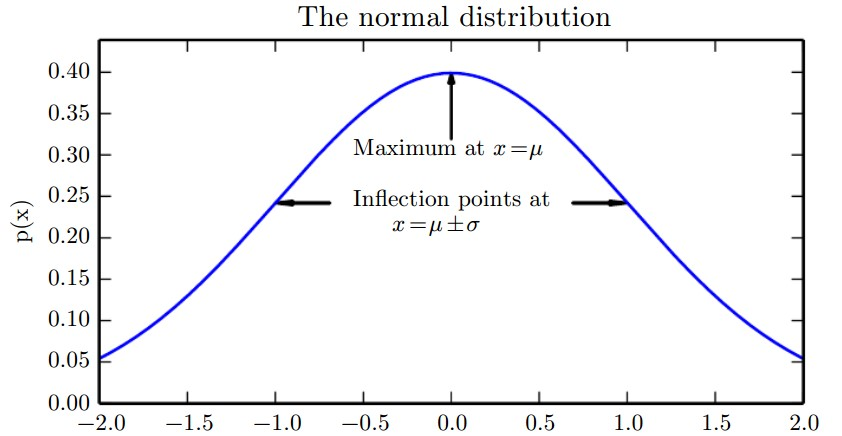
\includegraphics[width=3.5in]{fig/chap3/3_1.jpg}}
   \label*{图:3.1}
   \end{figure}
   \paragraph{}
    图3.1为正太分布密度函数的一个描述。正态分布是典型的钟形曲线,$\mu$为x轴的中间峰值。宽度由$\sigma$控制。此图中的例子,是一个$\mu$ 为0,$\sigma$为1的正太分布。
    \paragraph{}
    正太分布用两个参数$\mu\in \mathrm{R}$和$ \sigma\in (0,\infty)$ 来描述。参数μ 为中心峰值坐标。同样它的方差$E(\mathrm{x})= \mu$,用$\sigma$表示标准差, $\sigma^{2}$表示方差。
    \paragraph{}
    当我们计算概率密度函数的时候,我们需要对$\sigma$进行平方和取倒数。当我们需要频繁的使用不同的参数去计算概率密度函数的时候,我们可以引入一个参数$\beta\in (0,\infty)$ 控制正太分布的精度和逆方差来更有效的参数化正太分布。
   \begin{equation}
      N(x,\mu,\beta^{-1})=\sqrt{\frac{\beta}{2\pi}}\mathrm{exp}(-\frac{\beta}{2\pi}(x-\mu)^{2})  \tag{3.22}
    \end{equation}
    \paragraph{}
    许多情况下使用正太分布是一种分成明智的选择。在没有先验知识的情况下,采用正太分布是非常好的选择有以下两个原因:
    \subparagraph{}
    第一,我们希望模型的许多分布能真正接近正常分布。中心极限定理表明,许多独立的随机变量的总和是近似正态分布的。这就意味着在实际实践中,许多复杂的系统可以成功地建模为正态分布,即使该系统可以被更结构化的去分解。
    \subparagraph{}
    第二,可能的大部分概率分布具有相同的方差,而正态分布对实数的最大不确定度进行编码。因此,我们可以认为正态分布是一个最少将先验知识插入到模型中的一种分布。充分开发和证明这个想法需要更多的数学工具。此部分见章节19.4.2。
    \paragraph{}
    正太分布推广到$\mathrm{R}^{n}$,在这种情况下,它被称为多元正态分布。可以被一个正定对称矩阵$\sum$进行参数化。
    \begin{equation}
      N(x,\mu,\sum)=\sqrt{\frac{1}{2\pi^{n}\mathrm{det}(\sum)}}\mathrm{exp}(-\frac{1}{2}(x-\mu)^{T}\sum^{-1}(x-\mu))  \tag{3.23}
    \end{equation}
    \paragraph{}
    此处的$\mu$的意思和前面的是一样的,只不过现在是个向量。参数$\sum$给出了次分布的协方差矩阵。对于单因素情况下,当我们希望去计算不同参数值的概率密度函数的时候,协方差是不是一个有效的方式计算的参数化的分布。因此我们需要对$\sum$进行转置去评估概率密度函数。我们可以用一个精度矩阵$\beta$来替换。
    \begin{equation}
      N(x,\mu,\beta^{-1})=\sqrt{\frac{\mathrm{det}(\beta)}{2\pi}}\mathrm{exp}(-\frac{\beta}{2\pi}(x-\mu)^{T}(x-\mu))  \tag{3.24}
    \end{equation}
    \paragraph{}
    我们经常将协方差矩阵修正伪对角矩阵。更简单的一个例子,各向同性的高斯分布,其协方差矩阵是系数位常数的单位矩阵。
    \subsection*{3.9.4 指数分布和拉普拉斯分布}
    \paragraph{}
    在深度学习中,我们经常希望在x = 0的有一个尖锐点的概率分布。要做到这一点,我们可以使用指数分布:
    \begin{equation}
      p(x;\lambda)=\lambda1_{x\geq0}\mathrm{exp}(-\lambda x)  \tag{3.25}
    \end{equation}
    \paragraph{}
    指数分布采用函数$1_{x\geq0}$ 表示分配概率为零的X的所有负值.而拉普拉斯分布则是可以让概率在点$\mu$处取得峰值。
    \begin{equation}
     \mathrm{Laplace}(x;\mu;\gamma)=\frac{1}{2\gamma} \mathrm{exp}(-\frac{|x-\mu|}{\gamma}) \tag{3.26}
    \end{equation}
    \subsection*{3.9.5 狄拉克分布和经验分布}
    \paragraph{}
    在某些情况下,我们希望指定的概率分布在围绕某个点的集群中。那么呢,我们可以通过定义一个狄拉克$\delta$函数实现。
    \begin{equation}
      p(x)=\delta(x-\mu)  \tag{3.27}
    \end{equation}
    \paragraph{}
    狄拉克$\delta$函数定义为在除了零以外的点函数值都等于零,而其在整个定义域上的积分等于1。狄拉克$\delta$函数不像一个普通的函数,一个输入得到一个真正的输出。相反狄拉克$\delta$函数它是一种不同类型的数学对象,称为广义函数,他是根据属性的集成定义的。我们可以认为狄拉克$\delta$函数的目的就是把除$\mu$点以外的值都无限接近于0。
    \paragraph{}
    通过定义$P(x)$是$\delta$函数平移$-\mu$所得到的无限窄的一个函数,在$x=\mu$ 时值取无限大。狄拉克分布是经验分布的一部分,把概率的$1/m$分布在每个$m$点$x^{(1)}...x^{(m)}$上形成一个给定的数据集或样本集合。
    \begin{equation}
     \hat{p}(x)=\frac{1}{m}\sum_{i=1}^{m}\delta(x-x^{(i)}) \tag{3.28}
    \end{equation}
    \paragraph{}
    在经验分布的连续型变量中使用狄拉克分布是有必要的,但是在离散型变量中,情况就简单许多。在离散型变量中,可以慨括为多项分布,与每个可能的输入值相关联的概率,简单地等于在训练集的该值的经验频率。我们可以把从训练样本数据集形成的经验分布看做成是对我们指定数据模型的训练。另外一种可以最大限度的提高训练数据的概率的可能性的经验分布参见5.5小节。
    \subsection*{3.9.6 混合分布}
    \paragraph{}
    结合其他简单分布去定义一种新的分布是挺常见的。组合分布的一个常见的方法是构造一个混合分布。混合分布是由几项分布组成的。在每个试验中,选择哪种成分的分布产生的样本,是从多项分布中抽样单位分量所决定的。
    \begin{equation}
      p(\mathrm{x})=\sum_{i}P(c=i)P(\mathrm{x}|c=i)  \tag{3.29}
    \end{equation}
    其中$P(c)$是对成员的多项分布。
    \paragraph{}
    在前面我们已经接触到了混合分布的一个例子。经验分布的实数部分就是使用狄拉克的一个混合分布。
    \paragraph{}
    混合模型是一种用来创建一个更复杂分布的简单策略之一。在16 章我们会更加详细的去介绍简单分布到混合分布的创建。混合模型使我们能分析出一个非常重要的概念,潜在变量。潜在变量是用在我们无法观测的一种随机变量。从混合分布的单位变量$c$就可以看出。潜在变量可以通过联合分布与$x$相关。在这种情况下,$P(\mathrm{x},c)=P(\mathrm{x}|c)P(c)$.其中$P(c)$是基于潜在变量的,而$P(\mathrm{x}|c)$ 可以根据可见变量和潜在变量去决定$P(\mathrm{x})$的形状,虽然没有参考隐藏变量,但是也能描述$P(\mathrm{x})$。
    \paragraph{}
    非常重要和常用的联合模型是高斯混合模型,其中$p(\mathrm{x}|c=i)$是高斯的。每个组成部分都有在自己单独的均值$\mu^{(i)}$和方差$\ sum^{(i)}$. 有些混合模型可能有更多的约束。例如:协方差可以通过约束$\sum^{(i)}=\sum\forall i$来共享成员。作为一个单一的高斯分布, 混合高斯模型可以为每个组件是对角或各向同性的协方差矩阵的约束。
    \paragraph{}
    除了均值和方差,高斯混合分布指定了每个$i$的先验分布$\alpha_{i}=P(c=i)$。先验是指已经知道$c$的情况下观察到$x$。 做一下对比,$P(c|x)$是一个后验概率,因为它在观察到$x$ 后才计算。高斯混合模型是常用的近似密度,因为任何平滑的密度都可以被多变量高斯混合模型近似。
    \begin{figure}[!htb]
    \centering
   \centerline{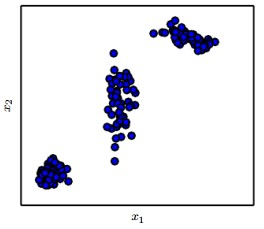
\includegraphics[width=3.0in]{fig/chap3/3_2.jpg}}
   \label*{图:3.2}
   \end{figure}
   \paragraph{}
   图3.2是高斯混合模型的样本。在这个例子中,有三个部分,从左到右,第一部分有一个各向同性的协方差矩阵,这意味着在每个方向上具有相同的方差。第二部分有一个对角协方差矩阵,这意味着它可以分别控制沿各轴方向的方差。从这个例子可以看出沿$X_{2}$轴的方差比$X_{1}$轴要大。第三部分有一个满秩的协方差矩阵,它能够单独控制任意方向上的方差。

    %--section 10--%

    \section*{3.10 常用函数的有用性质}
    \paragraph{}
    概率分布在很多函数的计算中应用广泛,特别是在深度学习模型中使用的概率分布。
    \paragraph{}
    这些函数之一就是描述S型曲线的logistic模型:
    \begin{equation}
    \sigma(x)=\frac{1}{1+\mathrm{exp}(-x)}   \tag{3.30}
    \end{equation}
    \paragraph{}
    S型曲线的logistic模型通常用于产生一个伯努利分布的参数$\varphi$,$\varphi$值的有效区间在(0,1)之间。图3.3是描述S型函数的图表,S型函数的参数过大或过小,都意味着函数变得平滑,且对其输入的微小变化不敏感。
    \paragraph{}
    另一个常见的函数是softplus 函数,参看(Dugas et al.,2001):
    \begin{equation}
    \zeta(x)=log(1+\mathrm{exp}(x))   \tag{3.31}
    \end{equation}
    \paragraph{}
    softplus 函数可以计算出正态分布的$\beta$和$\sigma$参数,其范围在$(0,\infty)$之间。当涉及S型曲线时常用该表达式。softplus 函数的名字来自于一个平滑的或"软化"版的如图3.4所示的softplus 函数的图表。
    \begin{figure}[!htb]
    \centering
   \centerline{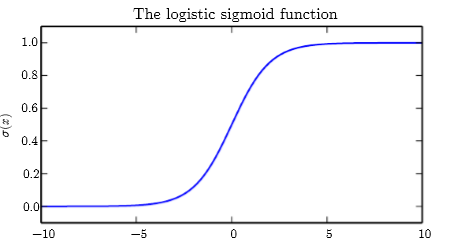
\includegraphics[width=3.5in]{fig/chap3/3_3.png}}
   \label*{图:3.3}
   \end{figure}
    \begin{figure}[!htb]
    \centering
   \centerline{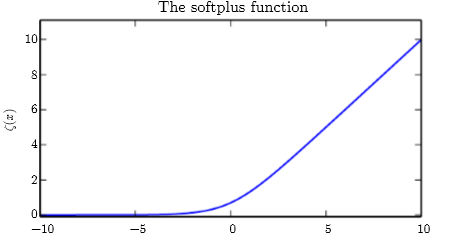
\includegraphics[width=3.5in]{fig/chap3/3_4.png}}
   \label*{图:3.4}
   \end{figure}
   \paragraph{}
   该函数具有以下性质:
   \begin{equation}
    \sigma(x)=\frac{\mathrm{exp}(x)}{\mathrm{exp}(x)+\mathrm{exp}(0)}   \tag{3.33}
   \end{equation}
   \begin{equation}
    \frac{d}{dx}\sigma(x)=\sigma(x)(1-\sigma(x))   \tag{3.34}
   \end{equation}
   \begin{equation}
    1-\sigma(x)=\sigma(-x)   \tag{3.35}
   \end{equation}
   \begin{equation}
    log\sigma(x)=-\zeta(-x)   \tag{3.36}
   \end{equation}
    \begin{equation}
    \frac{d}{dx}\zeta(x)=\sigma(x)  \tag{3.37}
   \end{equation}
   \begin{equation}
   \forall x\in(0,1),\sigma^{-1}(x)=log(\frac{x}{1-x})  \tag{3.38}
   \end{equation}
   \begin{equation}
   \forall x>0,\zeta^{-1}(x)=log(\mathrm{exp}(x)-1)  \tag{3.39}
   \end{equation}
   \begin{equation}
   \zeta(x)=\int_{-\infty}^{x}\sigma(y)dy  \tag{3.40}
   \end{equation}
   \begin{equation}
   \zeta(x)-\zeta(-x)=x \tag{3.41}
   \end{equation}
   \paragraph{}
   函数$\sigma^{-1}(x)$被称为统计的Logit模型,但是该术语很少用在机器学习中。
   \paragraph{}
   公式3.41对"softplus"给出了新的解释。Softplus函数是一个正部函数的光滑版本,$x^{+} =max{0, x}$。正部函数是负部函数的对应,$x^{-} = max{0,-x}$。为了获得一个平滑的函数,类似负部函数可以使用$\zeta(-x)$。$x$可以通过正部函数和负部函数通过$x^{+}- x^{-} = x$ 来抵消,也可以利用$\zeta(x)$和$\zeta(-x)$之间的关系来抵消,如公式3.41。

    %--section 11--%

    \section*{3.11 贝叶斯法则}
    \paragraph{}
    通常我们知道$P(y | x)$的情况下想计算$P(x | y)$,这时,如果我们还知道$P(x)$,我们就可以通过贝叶斯法则得到结果:
    \begin{equation}
   P(x|y)=\frac{P(x)P(y|x)}{P(y)} \tag{3.42}
   \end{equation}
   \paragraph{}
   需要注意的是,当公式中出现$P (y)$时,通常可以用$P(y)=\sum_{x}P (y|x)P(x)$计算,因此我们不需要去了解$P(y)$。贝叶斯规则是直接从条件概率的定义中得出的,但是我们熟悉这个名字是因为许多文本中提及才知道的。Reverend Thomas Bayes在公式中发现了一个特殊的现象,因此将其命名为贝叶斯。这里所提到的贝叶斯公式是由Pierre-Simon Laplace发现的。

    %--section 12--%

    \section*{3.12 连续变量的技术细节}
   \paragraph{}
  以恰当的形式理解连续随机变量和概率密度函数需要概率论的一个被称为测量理论数学分支的发展。测量理论是超出了这本教科书的范围,但我们可以简要的勾勒出一些测量理论的问题来解决。
   \paragraph{}
   在3.3.2节,我们看到,一个连续向量值$x$在集合$S$的概率是$P(x)$的积分。而一些集合$S$的选择可能会产生矛盾。例如,它可以构建两个集合$S1$和$S2$,即$P(x\in S1)+ P(x\in S2)> 1$但$S1 \cap S2 = \phi$.。这些集合通常是由大量使用的实数的无限精度的构造,例如分形集合或将有理数集合定义的集合。测量理论的一个重要贡献是提供一个表征的集合,我们可以计算出没有遇到矛盾的概率。在这本书中,我们只集成了相对简单的描述,所以这方面的测量理论不需要特别关注。
   \paragraph{}
   对于我们而言,测量理论在描述定理方面是非常有用的,其应用于$R_{n}$最点但不适用于一些边缘事件。测度理论提供了一个严格的方式来描述一个点集小到可以忽略不计。这个点集被称为“测量零”,我们在这本书中没有正式定义这个概念。然而,对它的理解是非常有用的,一组测量零点在我们测量的空间中没有体积,例如,当填充的多边形有正测量时,在$R_{2}$的线上有一个测量零点。同样,一个单独的点有测量零点。任何一个可数集合,每个都会有测量零点(因此所有的有理数集有测量零点)。
   \paragraph{}
   测量理论的另一个有用的术语是“几乎无处不在”,也就是除了集合的测量零点,几乎拥有其他所有的空间的属性。因为异常占据了可以忽略的空间,所以它们可以被安全地忽略许多应用程序。概率论中的一些重要结果持有所有的离散值,但只持有“几乎无处不在”的连续值。
   \paragraph{}
   连续变量的另一个技术细节是处理连续的随机变量,这是一个相互确定的函数。假设我们有两个随机变量$x$和$y$,使得$y = g (x)$,其中$g$是一个可逆的、连续的、可微变换。人们可能会想到$p_{y}(y)=p_{x}(g^{-1}(y))$.其实不是这样的。
   \paragraph{}
   举一个简单的例子,假设我们有一个随机变量$x$和$y$,均为标量,假设$y = x /2,x \in U(0,1)$。如果我们使用规则的$p_{y}(y)=p_{x}(2y)$,除了区间[0,1/2],$P_{y}$为0,在这个区间为1。这意味着下式违反了概率分布的定义。
   \begin{equation}
     \int p_{y}(y)dy=\frac{1}{2}.\tag{3.43}
   \end{equation}
   \paragraph{}
   这种常见的错误是因为它没有考虑函数$g$所引入的空间的变形。回忆一下$x$在一个体积无穷小的区域$\sigma x$的概率是$p(x)\sigma x$。由于$g$可以扩大或收缩空间,$x$空间中的无穷小体积在$y$空间中可能有不同的体积。
   \paragraph{}
   如何纠正这个问题,我们返回标量的情况下。我们需要保证其属性:
   \begin{equation}
      |p_{y}(g(x))dy|=|p_{x}(x)dx|.\tag{3.44}
   \end{equation}
   \paragraph{}
   从这一点上解决,可以得到:
    \begin{equation}
      p_{y}(y)=p_{x}(g^{-1}(y))|\frac{\partial{(x)}}{\partial(y)}|.\tag{3.45}
   \end{equation}
   \paragraph{}
   也可以用:
    \begin{equation}
      p_{x}(x)=p_{y}(g(x))|\frac{\partial{g(x)}}{\partial(x)}|.\tag{3.46}
   \end{equation}
   \paragraph{}
   在更高的维度,衍生出雅可比矩阵的行列式—矩阵的每个元素为$J_{i,j}=\frac{\partial{x_{i}}}{\partial(y_{j})}$.因此,对于实数向量$x$和$y$,
   \begin{equation}
      p_{x}(x)=p_{y}(g(x))|\det{(\frac{\partial{g(x)}}{\partial(x)})}|.\tag{3.47}
   \end{equation}

    %--section 13--%

    \section*{3.13 信息论}
   \paragraph{}
  信息理论是应用数学的一个分支,涉及如何量化信号中存在多少信息的问题。它最初被发明研究的是离散的字母在嘈杂的通道发送信息,如通过无线传输的通信。在这种情况下,信息理论讲述了如何设计最佳的代码并使用不同的编码方案计算来自特定概率分布的消息的期望长度。在机器学习的背景下,我们也可以应用信息论对一些不适用连续变量的信息长度进行解释。这一领域是电气工程和计算机科学的许多领域的基础。在这本教科书中,我们主要是使用一些关键的思想,从信息论来描述概率分布或量化概率分布之间的相似性。关于信息理论更详细内容参考Cover and Thomas (2006)或者MacKay(2003)。:
   \paragraph{}
   信息论背后的基础是学习一个不太可能的事件发生的信息量远远多于学习一个可能的事件发生的信息量。一个信息说:“今天早上太阳升起”是一个无用的信息是没有必要发送的,但是一个信息说:“今天早上发生了一次日食”,这个信息非常丰富。
   \paragraph{}
   我们想用直观的形式量化信息,特别的:
   \paragraph{}
   1 可能事件所含的信息量较少,在极端情况下,一定发生的事件没有任何信息量。
   \paragraph{}
  2 不太可能的事件其信息量越大。
  \paragraph{}
  3 独立事件的信息量可以相加。例如,投掷硬币时发现硬币两次朝
   \paragraph{}
   为了满足这三个属性,我们定义了一个事件$\mathrm{X} = x$的自信息:
   \begin{equation}
     I(x)=-\log{P(x)}\tag{3.48}
   \end{equation}
   \paragraph{}
   在这本书中,我们用$log$表示自然对数,基为$e$。我们定义的$I(x)$单位是$nats$。一个$nat$是通过观测概率为$1 /e$的事件得到的信息量。其他书中可能使用底数为2的对数,单位为比特或香农;测量信息位只是一个$nats$的标度测量信息。
   \paragraph{}
   当$x$是连续的,我们使用相同定义的信息通过类比,但一些属性在离散的情况下丢失。例如,尽管不是一个保证发生的事件,其单位密度的事件仍然有零的信息。
   \paragraph{}
   如图3.5所示,这个图显示了如何分类相近的确定性的较低的香农熵(Shannon entropy),如何分类接近均匀分布的有高的香农熵。在水平轴上,我们绘制$P$,一个二进制随机变量的概率等于1。熵为$(p- 1) log(1- p) - p log p$。当$p$接近0时,分布几乎是确定性的,因为随机变量几乎总是0。当$P$接近1时,分布几乎是确定性的,因为随机变量几乎总是1。当$P$ = 0.5时,熵是最大的,因为分布是均匀的两个结果。
   \begin{figure}[!htb]
   \centering
   \centerline{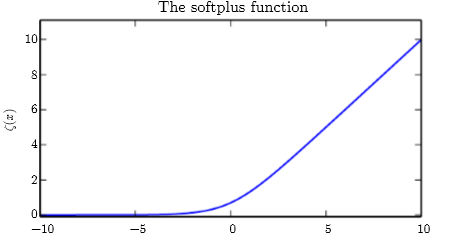
\includegraphics[width=3.5in]{fig/chap3/3_4.png}}
   \label*{图:3.5}
   \end{figure}
   \paragraph{}
   自我信息只处理一个单一的结果。我们可以使用香农熵在一个全概率分布下量化其不确定度。
   \begin{equation}
     H(x)=E_{(x\sim P)}[I(x)]=-E_{(x\sim P)}[\log{P(x)}]. \tag{3.49}
   \end{equation}
   \paragraph{}
   可以采用$H[P]$。换言之,一个分布的信息熵是来自该分布的事件的预期数量的信息。它给出了一个下界的比特数(对数以2为基础,否则单位是不同的)所需的平均编码符号服从一个分布$P$。分布几乎是确定性的(其中的结果是几乎肯定的)有低熵;有高熵的分布接近均匀。如图3.5。当$x$是连续的,其香农熵被称为微分熵。
   \paragraph{}
   如果我们有两个关于$x$的独立的概率分布$P(x)$和$Q(x)$,我们可以使用相对熵(Kullback-Leibler divergence,也称为KL散度)测量这两个分布的不同程度:
   \begin{equation}
     D_{KL}(P||Q)=E_{x\sim P}[\log{\frac{P(x)}{Q(x)}}]=E_{x\sim P}[\log{P(x)-\log{Q(x)}}].\tag{3.50}
   \end{equation}
   \paragraph*{}
   在离散型变量的情况下,它是一个额外的信息量(位测量时我们用以2为底的对数,但机器学习中我们通常使用$nats$和自然对数)需要发送一个包含来自概率分布$P$的符号的消息,我们可以使用一个准则最大限度地减少来自概率分布的消息的长度。
   \paragraph{}
   KL散度有许多有用的特性,最主要的是,它是非负的。KL散度为0表示在离散变量的情况下$p$和$q$的分布是相同的,等于一个无处不在的连续变量。因为KL散度是非负所以测量两个分布之间的差异,经常被理解为测量某种距离之间的分布。然而,它不是一个真正的距离测量,因为它不是对称的:对于$P$和$Q$,$D_{KL}(P||Q)\neq D_{KL}(Q||P)$。这种不对称性意味着对使用$D_{KL}$时选择$D_{KL}(P||Q)$ 和 $D_{KL}(Q||P)$ 哪一种对其结果影响很大。更多细节请参见图3.6。
   \paragraph{}
   和KL散度密切相关的是交叉熵,即$H (P,Q) = H(P) + D_{KL}(P||Q)$,这类似于KL散度,但如果缺少左边部分则:
   \begin{equation}
     H(P,Q)=-E_{x\sim P}\log{Q(x)}.\tag{3.51}
   \end{equation}
  \paragraph{}
  最小化相对于$Q$的交叉熵等价于最小化KL散度,因为$Q$和省略的$H(P)$不相关。
  \paragraph{}
  在计算这些量时,经常遇到0log 0这种表达形式。按照惯例,在信息论中,我们把这些表达式记为:$\lim_{x\rightarrow 0}x\log{x}=0$.
  \begin{figure}[!htb]
  \centering
   \centerline{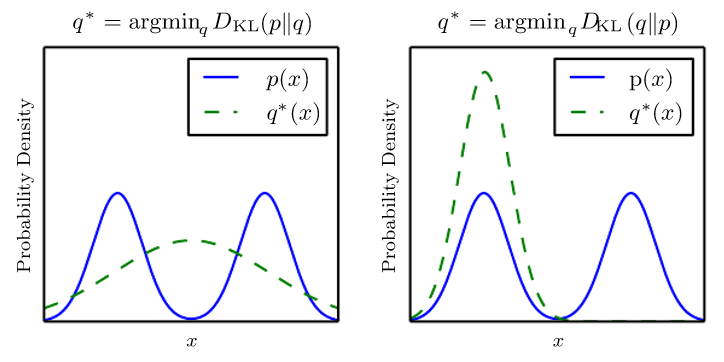
\includegraphics[width=5in]{fig/chap3/3_6.png}}
   \label*{图:3.6}
   \end{figure}
   \paragraph{}
   图3.6的KL散度是不对称的。假设我们有一个分布$P(x)$,并希望近似它与另一个分布$Q(x)$。我们要么选择最小化$D_{KL}(P ||Q)$ 或$D_{KL}(Q||P)$ 我们举例说明对$P$函数使用高斯混合计算和对$q$函数进行的高斯求解,这两种选择的不同影响。选择使用哪个方向的KL 散度是根据具体问题而言。一些应用需要一个近似,通常是高概率的任何地方,真正的分布位置的概率高,而其他应用程序需要一个近似,很少有地方高概率的真实分布的地方低概率。

    %--section 14--%

    \section*{3.14 构造概率模型}
  \paragraph{}
  在机器学习中使用概率分布通常会用到一大堆变量。通常情况下,这些概率分布只会与一部分变量直接相关。而使用一个单一的函数来描述整个联合概率分布是效率不高(无论是计算或统计方面)。
  \paragraph{}
  事实上,我们并不是使用一个单一的函数来表示一个概率分布,我们可以将一个概率分布分解成许多因素,然后相乘。例如,假设有三个随机变量:$A,B$和$C$。假设$a$影响$b$的值,$b$的影响$c$的值,但$a$和$c$相对$b$是独立的。我们可以这样来描述:
  \begin{equation}
   p(a,b,c)= p(a)p(b|a)p(c|b).\tag{3.52}
   \end{equation}
   \paragraph{}
   这样分解可以大大减少描述分布的参数。每个因数都在变量内引入了指数。这就意味着,如果我们能找到一个分解能用非常少的变量描述这个分布,那就可以大大减少描述一个分布的成本。
   \paragraph{}
   我们可以用图形来描述这些分解。这里我们用一个图形的理论,点的集合可用通过线来互联。当用图来表示因式分解的时候,我们把这个叫做结构化概率模型或图形模型。
   \paragraph{}
   有两种构造概率的模型:有方向的和无方向的。这两种图形模型使用一个图,用圆圈表示一个随机变量,一条线连接两个随机变量。用这样的方式来表示两个变量在概率分布中有直接的关系。特别的,一个有方向模型包含了分布所需的所有变量$x_{i}$,关联点的概率和它父节点的变量相关,父节点用$Pag(x_{i})$表示。
   \begin{equation}
   p(x)=\prod_{i}p(x_{i}|Pag(x_{i})).\tag{3.53}
   \end{equation}

   \paragraph{}
   无方向模型使用无方向的现将两个变量连在一块,它表示因式分解中的一系列函数。这些函数和有方向模型不同,它不是任何形式的概率分布。几个顶点连接起来叫做集合。每个集合$\mathcal{C}^{i}$在无方向模型中都会和一个因子建立关系$\phi^{(i)}(\mathcal{C}^{(i)})$,这些因子只是函数而非分布。要保证每个因子的输出都是非负的,不过不一定需要向概率分布那样,他们的和或积分为1.

   \paragraph{}
   随机变量的联合概率与所有这些因子的乘积成正比—对影响较大的因子,对其结果的影响也很大。当然,不能保证这种乘积的和一定为1。因此我们将通过除以常数$Z$进行归一化,为了获得一个归一化定义$\phi$函数产生的所有状态进行求和或积分。概率分布为:
   \begin{equation}
   p(x)=\frac{1}{Z}\prod_{i}{\o}^{(i)}(c^{(i)}) \tag{3.54}
   \end{equation}
   \begin{figure}[!htb]
   \centering
   \centerline{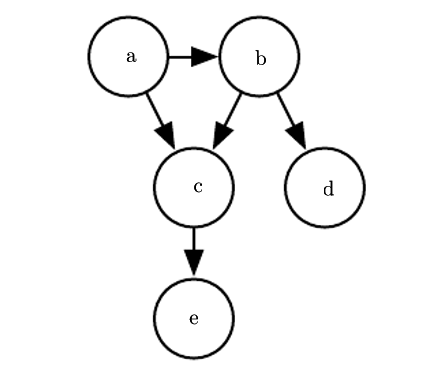
\includegraphics[width=2.5in]{fig/chap3/3_7.png}}
   \label*{图:3.7}
   \end{figure}
 \paragraph{}
 图3.7是一个有向模型的随机变量$a,b,c,d$和$e$。此图对应的概率分布可以分解为:
\begin{equation}
   p(a,b,c,d,e)=p(a)p(b|a)p(c|a,b)p(d|b)p(e|c).\tag{3.55}
 \end{equation}
\paragraph{}
 这个图可以让我们很快的看到一些分布的属性。例如,$a$和$c$之间直接影响,而$a$和$e$之间通过$c$间接影响。
 \begin{figure}[!htb]
 \centering
   \centerline{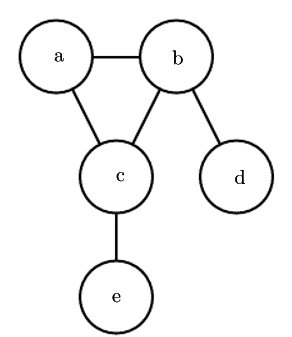
\includegraphics[width=2in]{fig/chap3/3_8.png}}
   \label*{图:3.8}
   \end{figure}
   \paragraph{}
   图3.8是一个无向模型的随机变量$a,b,c,d$和$e$。此图对应的概率分布可以分解为:
   \begin{equation}\
     p(a,b,c,d,e)=\frac{1}{Z}(a,b,c){\o}^{(2)}|(b,d){\o}^{(3)}(c,e).\tag{3.56}
   \end{equation}
   \paragraph{}
   这个图可以让我们很快的看到一些分布的属性。例如,a和c之间直接影响,而a和e之间通过c间接影响。
   \paragraph{}
   用这些图形表示分解是描述概率分布的一种语言。他们不是相互排斥的概率分布的成员。有向或无向不是一个概率分布的属性,它是一个概率分布的一个特定的描述,但任何概率分布都可以用这两种方式描述。
   \paragraph{}
   在这本书的第一部分和第二部分,我们将使用结构化的概率模型仅仅作为一种语言来描述直接概率关系和机器学习算法中的不同之处,没有进一步了解结构化的概率模型。直到讨论课题的第三部分中,我们将探索结构化概率模型中的更多细节。
   \paragraph{}
   本章回顾了深度学习相关的概率论的基本概念。其基本的数学工具仍然是:数值方法。

\end{CJK*}
\end{document}

%%%%%%%%%%%%%%%%%%%%%%%%%%%%%%%%%%%%%%%%%%%%%%%%%%%%%%%%%
%%%%%%%%%%%%%%%%%%%%% author:BrowningWan %%%%%%%%%%%%%%%%
%%%%%%%%%%%%%%%%%%%%% part:4.0-4.3       %%%%%%%%%%%%%%%%
%%%%%%%%%%%%%%%%%%%%%%%%%%%%%%%%%%%%%%%%%%%%%%%%%%%%%%%%%

\chapter{数值优化}
\label{chap:4}



\section{4.0}
%%%%%%%%%%%%%%%%%%%%%%%%%%%%%%%%%%%%%%%%%%%%%%%%%%%%%%%%
%%%%%%%%%%%%%%%%  author:cypress1010@sina.com %%%%%%%%%%
%%%%%%%%%%%%%%%%  part:4.4-4.5                %%%%%%%%%%
%%%%%%%%%%%%%%%%%%%%%%%%%%%%%%%%%%%%%%%%%%%%%%%%%%%%%%%%



\section{约束优化}
\label{sec:4.4}

我们不希望在$x$的所有可能取值内最大化或最小化函数$f(x)$,而是想要得到当$x$只在某个集合$\mathbb{S}$内时,$f(x)$的最大值与最小值。这就是有约束条件的优化,简称约束优化(constrained optimization)。在约束优化的专用术语里面,集合$\mathbb{S}$被称为可行域(满足约束条件的域),集合$\mathbb{S}$内的元素$x$被称为可行解。

我们通常希望得到一个在某种意义上较小的最优解,比较常用的方式是强制添加范数约束,如$\parallel{x}\parallel\leq1$。

梯度下降是一种解决无约束优化的最优化算法,为了解决约束优化问题,我们利用将约束条件考虑在内,然后利用改进的梯度下降算法。假定我们使用一个较小的恒定步长$\epsilon$,在梯度下降的每一步中,我们可以将结果投影到可行域$\mathbb{S}$上。如果使用的是直线搜索,我们就只能以步长为$\epsilon$搜索下一个可行解$x$,或者是同样可以把这条直线上的点投影到约束区域。对于直线搜索这种方法,如果先将梯度投影到可行域的切线空间,再进行梯度下降或者直线搜索,则效率会更高。

另外还有一种更加复杂的方法,对于某个约束优化问题,如果另有一个无约束优化问题的解能够被转换为该原始约束优化问题的解,那就可以直接用这个无约束优化替换该约束优化。例如,我们想要最小化$f(x)$,$x\in \mathbb{R} ^2$,并且$x$满足单位二范数约束,那么我们就可以构造关于$\theta$的函数$g(\theta)=f([cos\theta,sin\theta]^T)$,并将$[cos\theta,sin\theta]$作为原始问题$f(x)$的解。这种方法有一定的难度,因为要求两个优化问题之间的转换必须专门针对我们遇到的每种情况进行设计。

Karush-Kuhn-Tucker(KKT)\footnote{KKT方法是对拉格朗日乘子法的推广,拉格朗日乘子法只允许有等式约束}方法提供一种非常通用的解决方案,用来求解约束优化。为了熟悉KKT方法,在这里引入一个新的函数叫广义拉格朗日(genereralized Lagrange)或广义拉格朗日函数(genereralized Lagrange function)

为了便于定义拉格朗日函数,我们用等式与不等式来描述集合$\mathbb{S}$,如$m$个函数$g^{(i)}$和$n$个函数$h^{(j)}$,也即是说$S=\{x \ | \ \forall i,g^{(i)}(x)=0 \ and \ \forall j,g^{(j)}(x)\le0\}$
。这里$g^{(i)}$被称为等式约束(equality constraints),$h^{(j)}$被称为不等式约束(inequality constraints)。

同时,还为每一个约束分别引入变量$\lambda _i$与$\alpha _i$,这些变量被称为KKT乘子,广义拉格朗日函数的定义如下:

\begin{equation}
	L(x,\lambda,\alpha)=f(x)+\sum_{i}\lambda_i g^{(i)}(x)+\sum_{j} \alpha_j h^{(j)}(x)
\end{equation}


现在我们可以通过对此广义拉格朗日函数进行无约束优化,从而解决约束最小化问题。观察上面函数,只要至少存在一个可行解,并且$f(x)$的取值没有趋于无穷,那么就有

\begin{equation}
	\min\limits_{x} \max\limits_{\lambda} \ \max\limits_{\alpha,\alpha \geq 0} \ L(x, \lambda, \alpha)
\end{equation}

与下面函数具有相同的最优目标函数值,以及对应的$x$的最优解集合。

\begin{equation}
	\min\limits_{x \in \mathbb S} f(x)
\end{equation}

这种等价是成立的,因为只要满足约束条件,则有$\footnote{解释:因为有$h^{(j)}(x) \leq 0$,$g^{(j)}(x) = 0$,以及$a \geq 0$,因此当$\lambda$与$\alpha$均为$0$时,函数$L$取得最大值时,,所以$\max\limits_{\lambda} \max\limits_{\alpha, \alpha \geq 0} L(x, \lambda, \alpha) = f(x)$}$:

\begin{equation}
	\max\limits_{\lambda} \ \max\limits_{\alpha,\alpha \geq 0} \ L(x, \lambda, \alpha) = f(x)
\end{equation}

如果有任一约束无法满足,则有:
\begin{equation}
	\max\limits_{\lambda} \ \max\limits_{\alpha,\alpha \geq 0} \ L(x, \lambda, \alpha) = \infty
\end{equation}


%%因为有$h^{(j)}(x) \leq 0$,$g^{(j)}(x) = 0$,以及$a \geq 0$,因此当$\lambda$与$\alpha$均为$0$时,函数$L$取得最大值时,,所以$\max\limits_{\lambda} \max\limits{\alpha, \alpha \geq 0} L(x, \lambda, \alpha) = f(x)$

这一性质保证了不可行解不会成为最优解,同时可行域里面得到的最优解也不会改变。

为了得到约束优化的最大值,我们可以构造关于$-f(x)$的广义拉格朗日函数,从而可以导出如下优化问题:

\begin{equation}
	\min\limits_{x} \max\limits_{\lambda} \max\limits_{\alpha,\alpha \geq 0} -f(x)+\sum_{i}\lambda_i g^{(i)}(x) + \sum_{j}\alpha_j h^{(j)}(x)
\end{equation}

利用对偶,可以将上面式子转变为另一种形式,这种形式是在最外层完成最大化。

\begin{equation}
\max\limits_{x} \min\limits_{\lambda} \min\limits_{\alpha,\alpha \geq 0} -f(x)+\sum_{i}\lambda_i g^{(i)}(x) + \sum_{j}\alpha_j h^{(j)}(x)
\end{equation}

等式约束项前面乘子的符号无关紧要,既可以是正数也可以是负数,因为这里的优化对于每个$\lambda_i$的取值没有任何限制。

不等式约束相当有趣,当$h^{(i)}(x^*) = 0$,我们称约束$h^{(i)}(x)$处于活跃(active)状态,如果某个约束没有处于活跃状态,那么,删除掉这个约束后得到的解与有这个约束得到的解将至少有一个相同的局部解。不活跃状态的约束有可能会排除掉其它解,例如,对于可行域内的所有可行解都是最优解(代价相等的一块区域)的凸问题,可能会因为约束而删除掉某个子集,或者是一个非凸问题可能会有较好的驻点在收敛过程中被不活跃的约束排除掉。然而,不管是否包含了非活跃状态的约束,收敛后得到的一定是驻点。因为不活跃状态的约束$h^{(i)}$为负值,所以函数$\min\limits_\lambda \max\limits_\alpha \max\limits_{\alpha, \alpha \geq 0}L( \bm {x, \lambda, \alpha} )$必然有$\alpha_i = 0$。因此我们也能注意到,$\bm{ \alpha h(x) = 0 }$。换句话说,对于所有的$i$,至少要有一个参数满足$\alpha_i \geq 0$,并且$h^{(i)}(x) \le 0$的约束必须是处于活跃状态。为了更加直观的理解这一点,我们也可以说这个解是被不等式约束强加的边界,并且通过它对应的KKT乘子来影响$x$的解,或者是让不等式约束的KKT乘子为零,从而对最终解不产生影响。

广义拉格朗日函数的梯度为零;满足所有关于$x$和KKT乘子的约束;以及$\alpha \odot h(x) = 0$。这三个条件统称为$Karush-Kuhn-Tucker(KKT)$条件,描述了利用$KKT$乘子求解约束优化问题所需要满足的条件。

如果想了解更多关于$KKT$方法的相关知识,可以参考数值优化这本书(Nocedal and Wright(2006))。

\section{实例:线性最小二乘}
\label{sec:4.5}

假定我们想要得到最小化下面函数时$x$的取值
\begin{equation}
	f(x)=\frac{1}{2} \parallel Ax-b \parallel_{2}^{2}
\end{equation}

现在已经有一些特有的线性代数求解算法可以高效的解决这一类问题。然而,我们这里还是要探讨如何利用基于梯度的优化来求解,利用这样一个简单的实例来解释这种技术的工作原理。

首先,计算梯度:
\begin{equation}
	\delta_x f(x)=A^T (Ax-b) = A^T Ax - A^Tb
\end{equation}

然后,我们可以使用较小的步长沿着梯度下降,具体步骤参考算法4.1

\begin{algorithm}
	\caption{利用梯度下降最小化关于$x$的函数$f(x)=\frac{1}{2}\lVert Ax-b \rVert_2^2$}
	%%\label{alg1}
	设置较小的步长$\epsilon$和公差$(\delta)$,需要是正数。
	\begin{algorithmic}
		\WHILE{$\lVert \bm{ A^TAx - A^Tb} \lVert_2 > \delta$}
		\STATE $\bm{x \leftarrow {x}} - \epsilon\bm{(A^TAx - A^Tb)}$
		\ENDWHILE		
	\end{algorithmic}
\end{algorithm}


我们也可以用牛顿法求解,因为这个函数实质是一个二次函数,利用牛顿法进行二次近似足够准确,并且这种方法一步就能够收敛到全局最小。



假定我们想要最小化同样一个函数,只是把约束改为$x^T x \leq 1$。这样,我们就可以引入一个拉格朗日函数

\begin{equation}
	L(x, \lambda) = f(x) + \lambda ( x^T - 1 )
\end{equation}

到这里,上面的优化问题就转变为:
\begin{equation}
	\min\limits_{x} \max\limits_{\lambda, \lambda \geq 0} L(x, \lambda)
\end{equation}


这个无约束最小二乘问题的最小范数解可以使用Moore-Penrose伪逆(也可以称之为广义逆矩阵):$x=A^+b$,如果这个一个可行解,那它就是上述有约束优化问题的解。如果不是的话,则还需要找到某个约束处于活跃状态的解。将拉格朗日函数对$x$求导,可以得到如下方程:
\begin{equation}
	A^TAx - A^Tb + 2\lambda x = 0
\end{equation}

所以,最终的解会是如下形式:
\begin{equation}
	x = (A^TA + 2\lambda I)^{-1}A^Tb
\end{equation}

对于$\lambda$的取值,必须是要能够满足前面约束条件,我们可以通过对$\lambda$变量做梯度上升来得到取值,为了完成这一步,观察如下式子
\begin{equation}
	\frac{\partial}{\partial \lambda}L(x, \lambda) = x^Tx - 1
\end{equation}

当$x$的范数(这里是二范数)超过1时,上式的导数值大于0,为了沿着导数方向上山,并且增大关于$\lambda$的拉格朗日函数值,我们可以增大$\lambda$。由于$x^Tx$的惩罚系数变大,求解关于$x$的线性方程将能够得到一个较小的范数解,不断的求解线性方程并调整$\lambda$的值,直到$x$有正确的范数解以及关于$\lambda$的导数为0。

本章总结了开发机器学习算法过程中用到的一些数学基础,现在我们准备去搭建及分析一些成熟的学习系统。








\chapter{机器学习基础}
\label{chap:5}
%%%%%%%%%%%%%%%%%%%%%%%%%%%%%%%%%%%%%%%%%%%%%%%%%%%%%%%%%
%%%%%%%%%%%%%%%%% author:dormir_yin %%%%%%%%%%%%%%%%%%%%%
%%%%%%%%%%%%%%%%%%%%%%%%%%%%%%%%%%%%%%%%%%%%%%%%%%%%%%%%%

深度学习其实也是机器学习的一种方法。为了更好的理解深度学习,我们必须也要了解一下机器学习的基础知识。这章给大家简要介绍了机器学习中一些重要的概念,这些内容在本书的后续章节会涉及到。如果你是初学者或者想对机器学习有更广更详细的了解,推荐你找一本机器学习的教科书。比如说Murphy(2012)或者Bishop(2006)。如果你已经对机器学习的基础比较熟悉了,你可以直接开始看5.11。那部分内容介绍的传统机器学习技巧对深度学习算法的发展有较大的影响。

我们首先会先定义一下什么是机器学习算法。随后我们会给一个例子 线性回归算法。接着我们介绍拟合训练数据和将我们学习到的模型运用到新的数据集的不同之处。大部分机器学习算法会让我们设置超参数。这些超参数是需要我们自己定义的,而不能通过训练过程自动更新。我们也会讨论如何设置超参数。机器学习本质上就是应用统计学。和应用统计学不同的是它强调了了利用计算机来对一些复杂的函数进行统计估计。但是减弱了对估计出来的函数计算置信区间。就是说它利用统计学方法的得出一个模型,但它不强调用传统的假设检验的方式来对该模型进行评估。接着我们会介绍两个核心的统计算法 频率估计 和 贝叶斯推断。频率学派和贝叶斯学派也是统计学的两大流派。大部分机器学习任务可以分为监督学习和无监督学习两类。我们会对这两类做一个介绍,同时会介绍一些它们用到的机器学习算法。大部分深度学习算法是基于一种叫随机梯度下降法的优化算法。我们会介绍如何构建一个完整的机器学习算法。这些算法包含多个部分。优化算法,损失函数,模型和数据集。最后,在\ref{sec:5.11}我们介绍了传统机器学习算法遇到的一些困难,这些困难促使我们发展深度学习来解决传统机器学习算法所不能解决或者很难解决的问题。

\section{机器学习算法}
\label{sec:5.1}

所谓机器学习算法,就是能够从数据中学习的算法。但是学习到底是什么含义。Mitchell 提供了一个定义。一个计算机程序从关于不同类型的任务的经验中进行学习。

我们可以想象,经验 任务 还有评估策略可以有很多,在这本书中不会给这些名词一个正式的定义。但是我们在接下来的章节中会对他们进行大致的描述,并给一些例子来帮助大家这些名词,已经如何用它们来组成一个机器学习算法。

\subsection{任务 $T$}
机器学习可以解决一些传统的算法很难解决的问题,之前我们总会用人为设计的固定的算法来解决一些问题。从一个科学或者哲学的观点来看,机器学习之所以有趣,是因为在发展理解机器学习算法的同时,我们也会思考发现人类智能的本质。人是如何思考的。

在这一段,我们会给任务 T 一个相对正式的定义。学习本身的过程不能称之为任务,学习的目的是为了获得完成任务的能力。举个例子: 如果我们制作出了一个机器人,想让它具有走路能力,那么走路就是任务T。我们可以写一个程序让机器人自己学习如何走路,也可以直接写一个程序直接控制机器人走路。

机器学习任务通常机器学习系统如何处理一个个实例 Example。实例是特征的集合。这些特征来自于我们设计的机器学习系统需要处理的事件或者物体,而且都已经被量化了。我们通常把实例表示成一个向量,向量的每个元素表示不同的特征。比如说图像的特征通常就是图像的像素值。

机器学习可以解决很多不同的任务。下面我列举了最常见的机器学习任务:
\begin{itemize}
\item \textbf{分类:} 在这类任务中,总共有k类,计算机算法需要判断每个输入属于哪个类别。为了完成这个任务,学习算法通常需要产生一个函数,或者叫对应关系。模型会将每个输入x对应到某个类别y。当然也有很多类似的分类任务,比如说f输出一个概率分布,每个类别对应一个概率。物体识别就是分类任务的一个例子。这个任务重输入时一幅图片 通常可以描述成像素值的集合。输出是图片中物体对应的编码。比如说机器人 就可以识别不同的饮料,并把他们送给点单的客人。深度学习在完成目标检测都有较好的效果。同时,目标检测的算法也可以用于人脸识别,这样我们就可以对照片里的每个人进行自动标注了,而且也可以帮助计算机更好的和人类进行交互。

\item \textbf{缺失特征情况下的分类:} 如果一些数据缺失某些特征的化,分类问题会变得比较难。也就是说不能保证输入向量里每个对应的特征都可以提供。不同的x缺德特征也有可能不一样。传统的分类任务中,学习算法需要定义一个函数,能够将输入向量映射到一个输出类别。但如果一些输入特征缺失了,学习算法就需要定义一系列函数,

\item \textbf{回归:}  在这类任务重,计算机程序需要根据输入预测一下数值。为了解决这个问题,学习算法需要得到一个函数 这类人物和分类任务很像,唯一的不同就是输出的格式不一样,分类任务要求输出的是输入对应的类别,是离散的,而回归任务要求的输出是连续的数值。

\item \textbf{描述:}  在这类任务中,机器学习系统需要观察一些非结构化数据,然后用文字或者离散化的符号描述它们。比如说文字识别,计算机程序需要识别出图片中所包含的文字,然后将识别出来的文字返回。谷歌的 就是利用深度学习来街道号码的。另一个例子是语音识别,计算机程序会根据输入的波形来判断我们说的话。然后将它们转成文字或者文字对应的编码。现在深度学习是语音识别系统一个非常重要的组成部分,已经被好多大公司使用,包括微软,IBM,谷歌。

\item \textbf{机器翻译:}  在机器翻译任务中,我们需要将某种语言的序列翻译成另一种语言的对应的序列。这是自然语言处理的的一部分,比如说将音乐翻译成法语。深度学习在这些任务中,表现的越来越出色。
\item \textbf{结构化输出:} 这类任务一般都要求输出是一个向量,或者其他能够存储多个值的数据结构。这样的任务太多了,包括我们上面提到的描述和机器翻译。当然还有一些其他的任务,比如说将

\item \textbf{异常检测:}  在这类任务中,计算机程序会对输入的事件和目标进行筛选,找出那些异常的的事件或者事物。信用卡欺诈检测就是这类任务的一个例子。通过对你的消费习惯进行建模,当你的卡被盗刷的时候,信用卡公司可以检测出来这个异常事件。当小偷盗取了你的行用卡或者信用卡信息,他进行消费的时候,这些消费记录会和你的消费习惯的概率分布不一致。这样信用卡公司在检测到你的信用卡账号有异常购买记录的时候就会直接把你的信用卡给锁了。可以看一下,里面介绍了一些异常检测的方法。

\item \textbf{模仿合成及采样:}  在这类任务中,机器学习算法或生成一些和训练数据相似的数据。这类任务在艺术和多媒体领域很有用,艺术家进行创造的过程是很枯燥的,而且要花费大量的经历。比如说,在电脑游戏中,我们可以自动生成一些物品和风景。而不是依靠艺术家一点一点画出来。当然我们也可以接收一些比较特殊的输入。比如说语音合成,我们输入一个句子,然后程序就会合成这个句子对应的语音波形。这也是上文提到的结构化输出任务,但是在这个任务中每个输入并没有对应的唯一的正确的输出。我们期望输出会有多一点的变化,这样就会让人感觉更加自然和真实。

\item \textbf{缺失值预测:} 在这类任务中,机器学习算法我们会输入给机器学习算法一个数据实例,但是它的某些元素是缺失的。这个算法必须对这些缺失值作出预测。

\item \textbf{去噪:} 在这类任务中,我们会给学习器一个被污染的数据,这个被污染的数据是原始的纯净数据经过一个未知的污染过程所得到的。学习器必须从这个被污染的数据中预测出原始的那个纯净的数据。或者说,预测出条件概率分布。

\item \textbf{密度估计和概率质量函数估计:} 在密度估计的问题中,机器学习算法需要学习一个函数。x从某个概率分布空间采样出来的数据。当x是连续变量的时候, 可以被看做是密度函数。当x是离散的时候,这个可以被看成一个概率质量函数。为了完美的完成这个任务 当然如何评价模型的好坏我们会在下面一个小结来讨论。这个算法需要我们学习数据的分布,我们需要知道哪些地方出现的数据多,哪些范围数据很少出现。这些任务需要学习算法可以得到数据分布的信息。我们可以通过对这些分布信息进行计算处理来完成其他任务。比如说我们通过概率估计获得了概率分布px,我们可以使用这个结果来解决上面提到的缺失值预测任务。如果缺失了,但是我们有其他的值。这样我们就知道缺失值得条件概率分布式 。在实际应用中,密度分布估计不能总是帮助我们解决这些相关的问题。因为很多情况我们需要通过px来做的一些计算是很难的。
\end{itemize}

当然,还有很多其他类型的任务。我们在这列了这么多只是想告诉大家机器学习能做的一些例子。这些并不是一个严格的任务的分类。


\subsection{评估准则 $P$}
为了能够对机器学习算法进行评估,我们需要针对模型的表现设计一些可以量化的评价准则。通常针对不同的任务我们会设计不同的评价准则。
对于分类任务,有缺失值得分类任务,识别任务我们使用精度来评价模型。精度就是那些模型给出正确输出的数据所占的比例。我们也可以通过计算错误率来获得同样的信息。错误率和模型相反,是模型给出错误输出的数据所占的比重。这个错误率也可以看做是01损失。在某个特定的数据例子上,如果被正确分类了,那么损失是0,否则损失是1. 但是对于概率密度估计这类任务,估计精度就,错误率或者其他类似01损失就没有意义。我们需要找一个新的评估准则来对每个数据点一个分数,这个分数的取值范围是连续的。最常用的方法就是通过模型来给每个数据点赋予一个平均对数概率。
通常我们比较重视模型的泛化性,也就是说看这个模型在处理它之前没见过的数据上面的表现。这个表现可以看出它在实际使用中是否可以工作的很好。因此,我们会通过一个测试集来评估模型,这个测试集是从我们之前用于训练模型的数据集里面分离出来的。
我们的评估准则可能看上去很直接。但是我们其实很难给系统选择一个评估准则可以真正符合我们的要求。
在一些情况下,我们很难决定我们需要评估什么。举个例子,在描述任务中,我们评估精度的时候,我们应该考虑整个序列,当整个序列都正确我们才算对,还是使用一个更细致的评估准则,当序列中某一部分对的时候,我们也给一点分,而不是直接给零分。在回归任务中,对于两个系统,一个会经常发生一些小错误,一个偶尔会发生一些大错误。我们会更偏向哪个呢,或者说准备给那个系统一个更大的惩罚。我们要根据我们的实际需求来作出选择。
在其他一些情况下,我们可以明确需要评估的对象。但是评估的过程不是很方便。举个例子,在概率密度估计的任务中经常会遇到这些问题。很多最好的概率模型表示的概率分布是暗含的,如果你想计算空间中某个特定点的概率值在这些模型中是不可以的。在这种情况下我们需要重新设计一些规则,使我们目标。或者设计一个和理想规则的近似规则。



\subsection{经验 $E$}
根据在学习过程中可以允许获得的经验的类型,机器学习算法可以直接分成监督学习和无监督学习。

这本书介绍的大多数机器学习算法可以被理解成能够接触整个数据集。在511 ,我们已经定义了一个数据集就是很多数据实例的集合。数据实例我们有时候也叫他数据点。

鸢尾花数据集就是一个相当古老的数据集,很早就被统计学家和机器学习研究者来使用。这个数据集记录了鸢尾花不同部分的数据。总共记录了150株鸢尾花,每一株就是一个数据实例。数据实例里面的特征对应的就是鸢尾花不同的部分。萼片长度,萼片宽度,花瓣长度,花瓣宽度。数据集还记录了每个鸢尾花对应的类别。总共有3种不同的鸢尾花类别。

无监督学习算法会遍历整个数据集,一般这个数据集包含很多特征。算法会从数据集的结构中学习其中有用的属性。在深度学习中,我们通常想学习产生数据集的概率分布。判断这个目标函数是不是很直接,类似于概率密度估计。或者是类似于合成,去噪之类的任务。目标不是很明显。还有一些其他的无监督学习算法,比如说聚类,就是根据数据实例的相似度将数据集分成几类。

监督学习算法的数据集也有很多特征,但是每个数据实例都会对应一个标签。比如说鸢尾花集里的每个数据实例就对应某种鸢尾花的类别。一个监督学习算法可以学习整个鸢尾花集,随后就可以将新的数据分成三种不同的鸢尾花类别。

简单的来说,无监督学习会观察几个实例$x$,这几个实例一般都是随机向量。并且会从这些数据集中来学习概率分布$p(x)$,或者这个分布中其它的一些性质。在监督学习里,也会观察一些实例x,但是,每个实例都有一个对应的值或者向量。我们需要通过通过$x$来预测$y$。通常我们会使用$p(y,x)$来进行估计。我们之所以叫监督学习是因为我们会提供一个目标值$y$。就好像是有一个老师来教机器学习系统该如何去做。在无监督学习中,并没有什么老师,机器学习算法需要独自理解数据的内容,或者从中发现一些有趣的东西。
监督学习和非监督学习并没有一个正式的定义。它们之间的界限也比较模糊。很多机器学习算法既可以做监督学习任务,也可以做非监督学习任务。举个例子,在概率图中有一个链式法则:给定一个向量$x$,它的联合分布可以被分解成:

表面上看求联合概率密度是一个非监督学习任务,但是通过这个分解我们把求联合概率px的任务分解成了n个监督学习的问题。相反,当我们想解决监督学习问题$p$ 我们可以通过传统的无监督学习的的技术来学习$x$,$y$的联合分布然后我们就可以用贝叶斯公式来解决这个问题:

\section{算法容量,过拟合,欠拟合}
\label{sec:5.2}

\section{超参数和验证集}
\label{sec:5.3}

\section{估计,偏差,方差}
\label{sec:5.4}

\section{最大似然估计}
\label{sec:5.5}

\section{贝叶斯统计}
\label{sec:5.6}
%%%%%%%%%%%%%%%%%%%%%%%%%%%%%%%%%%%%%%%%%%%%%%%%%%%%%%%%%
%%%%%%%%%%%%%%%%%%% author:KaiserW %%%%%%%%%%%%%%%%%%%%%%
%%%%%%%%%%%%%%%%%%% part:5.7-5.11  %%%%%%%%%%%%%%%%%%%%%%
%%%%%%%%%%%%%%%%%%%%%%%%%%%%%%%%%%%%%%%%%%%%%%%%%%%%%%%%%

\section{监督学习算法}
\label{sec:5.7}
前承\ref{sec:5.1.3}节,有监督学习(Supervised Learning)简单来讲就是一种学习算法,它会学着在某些输入和某些输出之间建立关联,这些输入\textbf{x}和输出\textbf{y}来自于训练集中的样本。很多时候,输出\textbf{y}很难自动采集,而必须由一位人工“监督者”(supervisor)提供,当然即便训练集的拟合目标已经自动采集完成,“监督学习”的名称仍然适用。
\subsection{概率监督学习}
\label{sec.5.7.1}
本书提到的大多数监督学习算法都是基于对概率分布$p(y|x)$的预测。我们可以简单地应用最大似然估计(maximum likelihood estimation)来找到分布$p(y|x;\theta)$参数族的最佳参数向量$\theta$。

已知线性回归(linear regression)对应参数族
\begin{equation}
	p(y|x;\theta) = \mathbb{N} (y;\theta^{T}, \textbf{\textit{I}})
  	\label{form:5.80}
\end{equation}

通过定义不同族的概率分布,我们可以将线性回归推广到分类(classification)情景。如果我们有两个类别,类0和类1,那么接下来只需确定其中一个类的的概率就可以了。类1的概率自然也就决定了类0的概率,因为两个概率值相加必然为1.
基于平均值将实数域上的正态分布进行参数化,这一分布我们也用于线性回归,这里的平均值可以是任意值。但是二元变量的分布则更加复杂一些,因为其平均值必然始终落在0和1之间。一种解决方案是应用逻辑函数(logistic function, 也称sigmoid函数)将线性函数的输出值挤压到(0,1)区间,转换后的值可以理解为是一个概率:
\begin{equation}
	p(y=1|x;\theta) = \sigma (\theta^{T}x)
  	\label{form:5.80}
\end{equation}

这一方法即是逻辑回归(logistic regression),这名字有些古怪,因为我们实际上用这个模型做分类而不是回归。
对于线性回归,我们可以解正规方程(normal equations)以求得最优权重。而逻辑回归就要复杂一些,它的最优权重没有解析解。我们只能通过最大化对数似然率(log-likelihood)来逼近最优解,具体的策略是,应用梯度下降法(gradient descent)使负对数似然率(negative log-likelihood, NLL)最小化。

这一策略基本可以应用在任何监督学习问题中:对于正确类型的输入/输出变量,写下其条件概率分布的参数族。

\subsection{支持向量机}
\label{sec:5.7.2}

支持向量机(Boser et al., 1992; Cortes and Vapnik, 1995)是最具影响力的监督学习方法之一。该方法与逻辑回归很相似,因为都是由线性函数$\omega^{T}x + b$所驱动。不同于逻辑回归,支持向量机(Support Vector Machine, SVM)并不提供概率值,只有分类结果。当$\omega^{T}x + b$为正,SVM预测为正类;同理当$\omega^{T}x + b$为负,则预测为负类。

支持向量机的关键创新点是\textbf{核技巧}(kernel trick)。核技巧观察到很多机器学习算法可以写作样本的点乘积。例如,支持向量机所用的线性函数可以写作形如
\begin{equation}
	\omega^{T}x + b = b + \sum_{i=1}^{m}{\alpha_{i}x^{T} x^{(i)}} 
    \label{form:5.81}
\end{equation}

这里$x^{(i)}$是一个训练样本,$\alpha$是系数矢量。

以这种方式重写学习算法之后,我们便可以用特征函数$\phi(x)$的输出和函数$k(\textbf{x}, \textbf{x}^{(i)})=\phi(\textbf{x})\cdot\phi(\textbf{x}^{(i)})$替代$\textbf{x}$,其中的$k(\textbf{x}, \textbf{x}^{(i)})=\phi(x)\cdot\phi(\textbf{x}^{(i)})$就叫做\textbf{核}(kernel)。$\cdot$操作符表示与$\phi(x)^{T}\phi(\textbf{x}^{(i)})$类似的内积。在有些特征空间中,我们可能无法使用真正的矢量内积;在有些无限多维的空间中,我们需要使用其他类型的内积,比如基于积分而不是加法的内积。此类内积的完整推导已经超出了本书的范畴。

用核替代了点积之后,我们可以用以下函数做预测
\begin{equation}
	f(x) = b + \sum{i}^{}{\alpha_{i}k(x,x^{(i}}
	\label{form:5.82}
\end{equation}

此函数对$textbf{x}$是非线性的,但是$\phi(\textbf{x})$和$f(\textbf{x}$之间是线性关系。并且$\alpha$和$f(\textbf{x}$也是线性关系。以下过程与基于核的方程都是严格等效的:对所有输入应用$\phi(\textbf{x}$,然后在新的变换空间中学习线性模型。

核技巧的强大有两重原因。首先,它允许我们并使用保证有效收敛的凸优化(convex optimization)技术,把对$x$的非线性函数当作线性的来学习。这是因为我们认为$\phi$是不变的,只优化$\alpha$,换言之,优化算法可以把决策方程在另一个空间中看作线性的。其次,相比于直接构建两个$\phi(\textbf{x})$矢量并显式求点积,核函数$k$的计算效率往往更高。

某些情况下,$\phi(\textbf{x})$甚至可以是无限维的,直接的显式求解将导致无穷的计算消耗。多数情况下,$k(\textbf{x}, \textbf{x'})$是$\textbf{x}$的非线性可解函数,即使$\phi(\textbf{x})$不可解。作为无限维特征空间中可解核的例子,我们构建一个特征映射,从非负整数x到$\phi(\textbf{x})$,设想该映射返回一个包含x个1及无穷多个0的矢量。我们可以写一个核函数$k(\textbf{x}, \textbf{x'}) = min(x, x^{i})$,这与无限维的点积严格等价。

最常用的核是高斯核(Gaussian kernel)
\begin{equation}
	k(u, v) = \mathbb{N}(u-v;0, \sigma^{2}I)
\end{equation}
$\mathbb{N}(x;\mu,\Sigma)$是标准正态密度。这个核也被称为径向基函数(radius basis function, RBF)核,因为其值随着


\section{非监督学习算法}
\label{sec:5.8}

\section{随机梯度下降法}
\label{sec:5.9}

\section{构建机器学习算法}
\label{sec:5.10}

\section{深度学习算法的动力}
\label{sec:5.11}
\part{深度学习:实战}
\label{part:2}

本部分将介绍可以用于解决实际问题的现代深度学习方法。


深度学习拥有着漫长历史和许多的应用,一些尝试至今已硕果累累。一些看起来野心十足的目标已经变为现实。深度学习中仍需探索的分支我们将留到最后一部分进行介绍。


本部分只介绍那些在工业中进行应用实践并获得成功的方法。


现代深度学习为有监督学习提供了一个十分强大的框架。通过增加层数或层间的单元数,网络可模拟更为复杂的函数。许多任务中都有把一个向量映射到另一个向量的工作,人类对这类工作翻译十分迅速,如果给出足够大的模型和大量的标签数据,深度学习也可以很好的完成这项工作。另外那些非向量映射可以描述的困难工作,甚至人类都需要时间思考和反应的,目前是不在深度学习讨论的范畴内。


本部分将讨论参数方程近似技术,这几乎要被所有的现代深度学习实践所使用。我们先介绍用于描述这些方程的前馈深度网络模型,然后我们会介绍正则化和优化等进一步的技术。缩放这些模型,使之适应于高分辨率的图像和长时间序列则需要进一步的讲述。我们将会介绍可用于缩放图像的卷积网络和处理时间序列的循环神经网络。最后,我们将总结一些可用于具体实践的指导,包括设计、构建、配置深度学习等,并对一些深度学习应用进行回顾。


本部分的章节对实践者来说最为重要,实践者们将开始使用深度学习技术解决真实世界中的问题。

\chapter{深度前馈网络}
\label{chap:6}
%%%%%%%%%%%%%%%%%%%%%%%%%%%%%%%%%%%%%%%%%%%%%%%%%%%%%%%%%
%%%%%%%%%%%%%%%%%% author:jim1949@163.com %%%%%%%%%%%%%%%
%%%%%%%%%%%%%%%%%% part:6.0-6.2           %%%%%%%%%%%%%%%
%%%%%%%%%%%%%%%%%%%%%%%%%%%%%%%%%%%%%%%%%%%%%%%%%%%%%%%%%

%%
\emph{正则度前馈网络}又被称为\emph{前馈神经网络}或\emph{多层感知机}(MLP), 是一种典型的深度学习模型。
一个前馈神经网络的目标是近似一个函数$f^*$。
例如,对于一个分类器而言,$y=f^*(\bm{x})$将x映射到类别$y$。一个前馈网络定义了一个映射$y=f(\bm{x};\bm{\theta})$, 并且学习了导致产生最好的近似函数的参数$\bm{\theta}$的值。

这些模型被叫做是\emph{前馈},因为信息通过从输入$\bm{x}$产生的方程,到用来定义f的中间计算,最后流向输出$\bm{y}$。这里没有那种模型的输出最后输入给自己的\emph{反馈}联系。当扩展了的反馈神经网络包含了反馈节时,他们被叫做\emph{前馈神经网络}(\emph{recurrent neural networks}),这会在第10章将会提到。

前馈网络对于机器学习的从业者及其重要。他们是形成很多重要商业应用的基础。例如,用于图像中的物体识别的卷积网络就是一种特别的反馈网络。前馈网络是在反复网络的道路上一个概念上的里程碑,它推动了很多自然语言的应用。

前馈神经网络被叫做/emph{网络}的原因是因为一般来说,它们被很多不同的方程组合所代表。这个模型与描述函数如何结合的直接循环图有关。例如,我们有3个函数$f^{(1)}$,$f^{(2)}$, 和$f^{(3)}$在链中相连,以形成$f^{(\bm{x})}=f^{(3)}(f^{(2)}(f^{(1)}(\bm{x})))$。
这些链式结构是最经常使用的神经网络结构。在这个例子里面,$f^{(1)}$被叫做神经网络的\emph{第一层},$f^{(2)}$被叫做\emph{第二层},以此类推。链条的总长给了模型的\emph{深度}。“深度学习”的名字就是从这个术语里面来的。前馈网络的最后一层叫做\emph{输出层}。在神经网络的训练中,我们训练$f^{(\bm{x})}$去匹配$f^*{(\bm{x})}$. 训练数据提供给我们有噪声的,估计的$f^*{(\bm{x})}$的例子,并且在不同的训练点被评估。每个例子$\bm{x}$都伴随一个标签$y\approx f^*(\bm{x})$。这些训练的例子直接给定了在每个点$x$输出层应该怎么做;它必须产生近似于y的值。其它层的表现没有被训练数据直接限定。学习算法必须决定如何水用那些层来得到理想的输出,但是训练数据没有说明每个独立的层应该做什么。相反,学习算法必须决定如何使用这些层来最好实现$f^*$的近似。因为训练数据没有展现每层的理想输出,这些层叫做\emph{隐藏层}(\emph{hidden layers})。

最后,这些网络被称作是\emph{神经}的原因是因为它们是基于神经科学基础的。网络的每个隐藏层一般是引入向量值的。那些隐藏层的维数决定了模型的\emph{宽度}。向量的每个元素可以解释成扮演一个类似于神经节的工作。不把层认为是简单的向量到向量的函数,我们也可以认为层由很多平行工作的\emph{单元}组成的,每个单元代表一个向量到标量的函数。每个单元像一个神经节一样,它从很多别的单元接受输入并且计算他自己的启动值。使用很多向量值代表层的想法来自于神经科学。用来计算这些代表的函数$f^(i)(\bm{x})$的选择,也被神经科学关于生物神经能计算的函数发现所引导。然而,现代的神经网络研究被很多数学和工程规则所指导,并且神经网络的目标也不是完美建模大脑。对于前馈网络的最好的认识是函数近似机器,它被设计成实现统计拟合,偶尔从我们对于大脑知道的部分获得一些灵感,而不是作为大脑函数模型。

一种理解前馈网络的方式,是从线性模型开始然后考虑怎样克服它们的缺陷。线性模型,例如逻辑回归和线性回归,就很有火因为它们可能会拟合地很有效和很可靠,要么在闭环方式要么是用凸优化的方式。线性模型也有一个明显的瑕疵:模型容量被线性函数所显,所以模型不能理解任意两个输入变量之间的交流。

为了将线性模型延伸到代表$\bm{x}$的非线性函数,我们可以应用线性模型不仅仅是$\bm{x}$自身,也可以是转换的输入$\phi(\bm{x})$,这里φ是非线性转换。相似地,我们可以应用5.7.2节描述的核心技巧,以得到基于含蓄应用$\phi(\bm{x})$映射的非线性学习算法。我们可以认为$\phi$作为提供一系列形容x的特征值,或者提供x$\bm{x}$的新代表。
问题是之后如何选择映射$\phi$。
\begin{enumerate}
\item 一种选择是使用一个非常通用的$\phi$,例如无限维的$\bm{\phi}$被隐含地用于基于$RBF$核的\emph{kernel machines}。如果$\phi(\bm{x})$有足够高的纬度,我们可以总是有足够的容量来拟合训练集,但是测试集的正则化经常保持不足。非常普通的特征映射,经常只是基于局部平滑,并且不对足够的先验信息编码解决高级的问题。
\item 还有一个方法是手工调制$\bm{\phi}$。这曾是主要的方法,直到深度学习的出现。这个方法要求对于不同的任务需要从业者人类的数十年的努力,需要参与者擅长不同领域例如语音识别或者机器视觉,并且在不同领域之间转换自如。
\item 深度学习的策略是学习$\phi$。在这种方法中,我们有模型$y=f(\bm{x};\bm{\theta}, \bm{\omega})=\phi(\bm{x}; \bm{\theta})^\top \bm{\omega}$。我们现在有参数$\bm{\theta}$去用来从一个很广义的函数类别里面去学习$\bm{\phi}$,和参数$\bm{\omega}$来从$\phi(\bm{x})$映射到期待的输出。这是一个深度前馈网络的例子,其中$\bm{\phi}$定义了隐含层。这个是唯有的三种方法之一,放弃了训练问题的凸性,但是好处更大。在这种方法中,我们把代表参数化为$\phi(\bm{x};\bm{\theta})$并且用优化算法来寻找$\bm{\theta}$以对应好的代表。如果我们希望,这个方法可以通过变得很通用来获得第一种方法的优势——我们通过使用一个很广泛集来做$\phi(\bm{x};\bm{\theta})$ 。这个方法也可以获得第二种方法的优势。人类从业人员可以将他们的知识编码来通过设计他们预计会表现良好的广泛集来帮助正则化。优势在于人类设计师只需要找出一般的合适函数集,而不用精确地找到正确的函数。
\end{enumerate}

这个通用的通过学习特征来改善模型的规则拓展了这章里面描述的前馈网络。这是个深度学习的复现的主题,适用于这本书里面描述的所有种类的模型。前馈网络是这种去学习决定性从缺乏反馈联系的$x$到$y$的映射的规则的应用。之后说的其它模型将会应用这些规则来学习随机映射,学习有反馈的函数,并且学习在一个向量上的概率分布。

我们从一个简单的前馈网络的例子来开始这章。然后,我们将会阐述每个设计决定来部署前馈网络。首先,训练前馈网络需要做出大量的和线性模型相同重要的设计决定:选择优化,成本函数,和输出形式。我们回顾这些基于梯度的学习的基础,然后进一步学习一些对于前馈网络特别的设计决定。前馈网络介绍了隐藏层的概念,并且这个要求我们去选择可以用来计算隐藏层值的\emph{激活函数}(\emph{activation functions})。我们也必须设计网络结构,包括网络里面有多少层,这些层应该怎么相互连接,以及每层里面有多少单位。学习深度神经网络需要计算复杂函数的梯度。我们提出\emph{反向传播}(\emph{back-propagation})算法和它的可以被用来有效计算梯度的现代正则化。最后,我们以一些历史层面来结尾。

\section{实例:学习XOR}
\label{sec:6.1}

为了让前馈网络的想法更加实际,我们先从一个例子开始,这个例子是用完全函数化的前馈网络来实现一个简单的任务:学习$\bf{XOR}$函数。

$\bf{XOR}$函数(“异或”)是两个二进制数$x_1$和$x_2$的运算。当正好这些二进制其中的一个数等于1,$\bf{XOR}$函数会返回1.否则,它会返回0。$\bf{XOR}$函数提供我们想要学习的目标函数$y=f^*(\bf{x})$。我们的模型提供函数$y=f(bf{x};bf{\theta})$并且我们学习的算法也会修改参数$\theta$,以使f尽可能接近$f^*$。

在这个简单的实例里面,我们不会担心数据正则化。我们想要我们的网络在四个点$\SetX=\{[0,0]^\top,[0,1]^\top,[1,0]^\top,[1,1]^\top\}$上正确地表现。我们将会在这四个点上面训练网络。唯一的挑战是拟合训练集。

我们可以把这个问题处理成回归问题,并且使用一个均方误差损失函数。我们用这个损失函数尽可能地来简化这个数学。我们将会在后面看的有对二进制数据建模的更合适的其它方法。

评估我们的全部训练集,$MSE$损失函数是
\begin{equation}
J(\theta)=\frac{1}{4} \sum_{\bf{x}\in \SetX} (f^*(\bf{x})-f(\bf{x};\bf{\theta}))^2
\end{equation}
现在我们必须选择我们的模型的形式,$f(\bf{x};\bf{\theta})$。假设我们选择一个线性模型,其中$\bf{\theta}$由$\bf{\omega}$和$b$组成。我们的模型定义成
\begin{equation}
J(\bf{x};\bf{\omega},b)=\bf{x}^\top \bf{\omega} + b 
\end{equation}

我们可以在封闭模式下最小化$J(\bf{\theta})$,对$\omega$和b使用正规方程。

在解完正常方程以后,我们获得$\bf{\omega}$=$\bf{0}$和$b=\frac{1}{2}$。每个地方线性模型都简单输出0.5。这个为什么发生呢?图 \ref{fig:6_1}展示了一个线性模型如何不能表示$\bf{XOR}$函数。一种方式去解决这个问题是使用一个模型,这个模型学习一个不同的特征空间,在里面一个线性模型能够体现解决方法。

特别地,我们将会介绍一个非常简单的前馈网络,其中有一个隐藏层包含两个隐藏单元。在图\ref{fig:6_2}中有这个模型的解释。这个前馈网络有一个隐藏单元$\bf{h}$,它是被函数$f^{(1)}(\bf{x};\bf{W},\bf{c})$。这些隐藏单元的值之后被用作第二层的输入。第二层是网络的输出层。输出层仍然只是一个线性回归模型,但是现在他将要应用到h上面而不是x。这个网络现在总共包含两个函数链:$\emph{h}=f^{(1)}(\bf{x};\bf{W},\bf{c})$和$y=f^{(2)}(\bf{h};\bf{\omega},b)$,其中有完整的模型是$f(\bf{x};\bf{W},\bf{c},\bf{\omega},b) = f^{(2)}(f^{(1)}(\bf{x}))$。

$f^{(1)}$应该计算什么样的函数呢?线性模型目前我们已经应用的很好了,并且可能最好也让$f^{(1)}$变成线性的。不幸的是如果$f^{(1)}$是线性的,那么前馈网络作为整体应该保持作为一个输入的线性函数。忽略掉目前的截距项,假设$f^{(1)}(\bf{x})=\bf{W}^\top \bf{x}$,并且$f^{(2)}(\bf{h})=\bf{h}^\top \bf{\omega}$。然后$f(\bf{\omega})=\bf{\omega}^\top \bf{W}^\top \bf{x}$。我们可以代表这个函数为$f(\bf{x})=\bf{x}^\top \bf{\omega’}$ 其中$\bf{\omega’}=\bf{W} \bf{\omega}$。


\begin{figure}[htbp] %  figure placement: here, top, bottom, or page
   \centering
   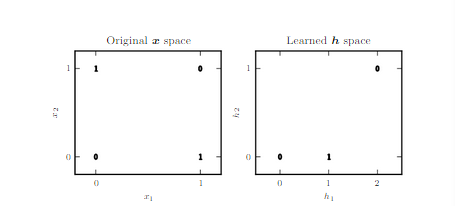
\includegraphics[width=6in]{fig/chap6/6_1.png} 
   \centering
   \caption{学习代表来解决$\bf{XOR}$问题。图像上打印的黑体字指出学习函数在每个点必须输出的值。(\emph{左边})一个线性模型直接应用到最开始的输入不能实现$\bf{XOR}$函数。当$x_1=0$,模型的输出必须随着$x_2$增长而增长。一个线性模型必须有适用于$x_2$一个固定的系数$w_2$。线性模型因此不能使用$x_1$的值来改变$x_2$上的系数,并且不能解决这个问题。(\emph{右边})在变换空间中,从神经网络中提取出由特征代表,一个线性模型现在可以解决这个问题。在我们的解决实例的方法中,必须有输出1的两点已经收缩成特征空间里面一个单独的点。换句话来说,非线性特征已经同时映射$\bf{x}=[0,1]^\top$和$\bf{x}=[0,1]^\top$到一个特征空间里面的一个单独的点,$\bf{h}=[1,0]^\top$。线性模型现在可以描述函数为在$h_1$中增长和在$h_2$中减少。在这个例子中,学习特征空间的动力只是为了使模型容量更大,这样它可以拟合训练集。在更现实的应用中,学习的代表也可以帮助模型正则化。}
   \label{fig:6_1}
\end{figure}


\begin{figure}[htbp] %  figure placement: here, top, bottom, or page
   \centering
   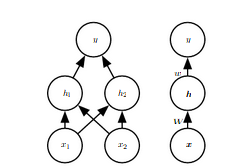
\includegraphics[width=6in]{fig/chap6/6_2.png} 
   \centering
   \caption{使用两种不同方式画出的,一个前馈网络的一个例子。特别地,这是我们用来解决$\bf{XOR}$例子的前馈网络。它有一个包含了两个单元的单隐藏层。(\emph{左边})用这种形式,我们在图中画出每个单元作为一个节点。这个形式是非常明确的和不含糊的,但是对于比这个例子大的网络,就会消耗太多的空间。(\emph{右边})在这个形式中,我们在图中画出一个节点对于每个整个的代表一层的激活部分的矢量。这个形式是更坚实的。有时候我们用描述两层关系的参数名称来注释图中的边缘。这里,我们指出矩阵$\bf{W}$描述着$\bf{x}$到$\bf{h}$的映射,然后向量$\bf{\omega}$描述着$\bf{h}$到$y$的映射。当给这种画图方法贴标签的时候,我们一般删除与各层相关的截距参数。}
   \label{fig:6_2}
\end{figure}

明显地,我们必须使用一个非线性的函数来表示特征。大多数神经网络通过已经学过的参数控制的仿射转换,以及叫作启动函数的一个固定的,非线性的函数做到这样。我们用这里的那个逻辑,定义$\bf{h}=g(\bf{W}^\top \bf{x}+\bf{c})$,这里$\bf{W}$提供了线性变换的权重以及$\bf{c}$作为偏置。之前,为了描述一个线性回归模型,我们用一个权重向量和一个标量偏移参数来描述一个从输入向量到一个输出向量的仿射变换。现在,我们描述一个从向量$\bf{x}$到向量$\bf{h}$的仿射变换,因此我们需要一整个向量的偏置参数。激活函数g一般被选作一个应用来元素加密的函数,有$h_i=g(\bf{x}^\top \bf{W}_{:,i}+c_i)$。在现代神经网络中,默认的推荐是使用在图\ref{fig:6_3}描述的由激活函数$g(z)=\max\{0,z\}$定义的\emph{rectified linear unit}或者ReLU(Jarrett et al., 2009; Nair and Hinton, 2010; Glorot et al., 2011a)。


我们现在可以明确完整的网络为
\begin{equation}
f(\bf{x};\bf{W},bf{c},bf{\omega},\bf{b})=\bf{\omega}^\top \max\{0,\bf{W}^\top \bf{x}+\bf{c}\}+b
\end{equation}

我们可以现在明确对于$\bf{XOR}$问题的解。设
\begin{align}
\bm{W} &= \begin{bmatrix}
1 & 1\\
1 & 1
\end{bmatrix},\\
\bm{c} &= \begin{bmatrix}
0\\
-1
\end{bmatrix},\\
\bm{w} &= \begin{bmatrix}
1\\
-2
\end{bmatrix},
\end{align}
并且b=0。

\begin{figure}[htbp] %  figure placement: here, top, bottom, or page
   \centering
   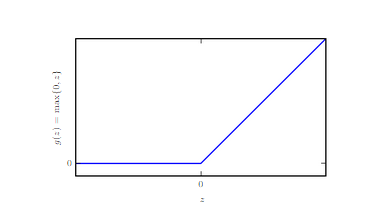
\includegraphics[width=6in]{fig/chap6/6_3.png} 
   \centering
   \caption{修正线性激活函数。这个激活函数是默认的推荐给大多数前馈神经网络使用的激活函数。应用这个函数到线性转换的输出,产生一个非线性转换。然而,这个函数仍然很接近于线性,也就是说他是有两段的分段线性函数。因为修复线性单元几乎是线性的,他们保护了很多的性能使线性模型正则好。一个通用的计算机的原则是我们可以从最小的部分里面构建复杂系统。就像图灵机的记忆一样,只需要能存储0或者1,我们可以从修正线性激活函数中,建造一个通用的函数近似器。}
   \label{fig:6_3}
\end{figure}

我们现在可以考虑让模型处理一批输入。让$\bf{X}$成为包含了二进制输入空间中所有4个点的设计矩阵,每个样例一行:
\begin{equation}
\bf{X}=\begin{bmatrix}
0 & 0\\
0 & 1\\
1 & 0\\
1 & 1
\end{bmatrix}
\end{equation}

在神经网络中第一步是将输入矩阵乘上第一层的权重矩阵:
\begin{equation}
\bf{X} \bf{W}=\begin{bmatrix}
0 & 0\\
1 & 1\\
1 & 1\\
2 & 2
\end{bmatrix}
\end{equation}

下一步,我们加上偏置向量$\bf{c}$,来获得
\begin{equation}
\begin{bmatrix}
0 & -1\\
1 & 0\\
1 & 0\\
2 & 1
\end{bmatrix}
\end{equation}

在这个空间里,所有的样例都在斜率为1的直线上。当我们在这条线上移动的时候,输出需要从0开始, 然后升到1,之后再降到0。一个线性模型不能实现这个函数。为了计算完每个样例的$\bf{h}$的值,我们应用修正线性变换:
\begin{equation}
\begin{bmatrix}
0 & 0\\
1 & 0\\
1 & 0\\
2 & 1
\end{bmatrix}
\end{equation}
这个变换已经改变了样例之间的关系。他们不再在单个线上了。就像图\ref{fig:6_1}所示,它们现在在一个空间中,这里线性模型可以解决问题。

我们通过乘上权重向量$\bf{w}$完成:

\begin{equation}
\begin{bmatrix}
0 \\
1 \\
1 \\
0
\end{bmatrix}
\end{equation}

神经网络已经从这批的每个样例中获得了正确的答案。

在这个样例中,我们简单地简化解,然后显示了它没有错误。在实际情况下,就会有很多的模型参数和很多训练样例,所以人们不能简单像我们这样猜到解。相反,一个基于梯度的优化算法可以找到会制造很少错误的参数。我们对于$\bf{XOR}$描述的解是在损失函数的一个全局最小值,所以梯度下降可以收敛到这个点。也有别的$\bf{XOR}$相同的解,梯度下降也可以找到。梯度下降的收敛点依赖于参数的起始值。在实际中,梯度下降一般不会找到像我们这里展示的一样的干净的,容易理解的整数解。

\section{基于梯度的学习}
\label{sec:6.2}

设计和训练一个神经网络和用梯度下降法训练任何其它的机器学习模型没有太大的区别。在\ref{sec:5.10}节里,我们描述了怎样去通过明确一个优化程序,一个代价函数和一个模型族来构建一个机器学习算法。

我们目前的线性模型和神经网络的最大的区别是神经网络的非线性造成大多数我们感兴趣的损失函数变成了非凸的。这意味着神经网络一般通过迭代的,基于梯度的仅仅驱使损失函数到一个很小的值的优化器来训练,而不是用来训练线性回归模型的线性方程解,或者用来训练逻辑回归或者SVMs的全局收敛保障的凸优化算法。凸优化收敛始于任何起始参数(理论上——实际上它有很强的健壮性但是会遇到数字问题)。随机的梯度下降应用到非凸损失函数没有收敛保障,并且是对于起始参数的值敏感的。对于前馈神经网络来说,初始化小的随机值的所有权重是重要的。偏置也许被起始化为0或者是小的正值。用来训练前馈网络和几乎所有其它的深度网络的迭代的基于梯度的优化算法将会在第八章被详细地描述,其中参数初始化将会被特别地在\ref{sec:8.4}节讨论。目前,不难理解训练算法几乎总是基于用梯度用各种方式来降低代价函数。这个特别的算法是梯度下降方法思想的提升和精炼,在\ref{sec:4.3}节有描述,并且,更具体的,通常是随机梯度下降算法的提高,在\ref{sec:5.9}节有介绍。

我们当然可以训练模型例如线性回归和有梯度下降的支持向量机,事实上当训练集极其大时这是很常见的。从这个观点来看,训练一个神经网络和训练任何其它的模型没有什么太大的区别。计算梯度对于神经网络来说有稍微有点复杂,但是仍然可以被有效和精确地完成。\ref{sec:6.5}节将会描述如何通过方向传播和方向传播算法的现代正则来得到下降。

正如其它机器学习模型一样,为了应用基于梯度的学习我们必须选择一个代价函数,并且我们必须选择如何代表模型的输出。我们现在重新回到这些在神经网络情景有特殊重点的设计考虑上来。

\subsection{代价函数}
\label{sec:6.2.1}

一个深度神经网络设计的重要方面是代价函数的选择。幸运的,神经网络的代价函数或多或少和其它参数模型,例如线性模型的代价函数一样。

在大多数情况,我们的参数模型定义了一个分布$p(\bf{y}|\bf{x};\bf{\theta})$并且我们简单使用最大可能性的原则。这意味着我们在训练数据和如代价函数一样的模型的预计之间使用交互熵。

有时候,我们使用更简单的方法,而不是预测一个完全在$\bf{y}$上的概率分布,我们仅仅预测一些条件为$\bf{x}$的$\bf{y}$的一些统计数字。特殊的代价函数允许我们去训练这些估计的预测值。

用来训练神经网络的整体的代价函数将会经常使这里描述的初始的代价函数和一个规则化因素结合。在第\ref{sec:5.2.2}节,我们已经见到了一些简单的用于线性模型的规则化的例子。用于线性模型的权值衰减方法也是直接适用在深度神经网络,并且是最受欢迎的正则化策略。更加高级的神经网络的正则化策略将在第7章中描述。

\subsubsection{使用最大似然法学习条件分布}
\label{sec:6.2.1.1}

大多数现代神经网络用最大似然来训练。这意味着代价函数是简单的负数对数似然,或者描述成训练数据和模型分布之间的交互熵。这个代价函数表示为

\begin{equation}
J(\bm{\theta})=-\SetE_{\mathbf{x}, \mathbf{y} \sim \hat{p}_\text{data}} \log p_\text{model} (\bm{y} \mid \bm{x})
\end{equation} 
代价函数的特殊形式依据$\log p_\text{model}$的特殊形式在模型之间中改变。上述方程的拓展通常产生不依靠模型参数的一些因子并且可能会被放弃。例如,正如我们在\ref{sec: 5.5.1}节看到的,如果$p_\text{model}(\bm{y}\mid\bm{x}) = \CalN(\bm{y};f(\bm{x};\bm{\theta}), \bm{I})$, 那么我们恢复均方误差代价,
\begin{equation}
J(\theta) = \frac{1}{2} \SetE_{\RVx, \RVy \sim  \hat{p}_\text{data}} || \bm{y} - f(\bm{x}; \bm{\theta}) ||^2 + \text{const},
\end{equation}

至少换算系数是$\frac{1}{2}$并且一个因子不依赖于$\bm{\theta}$。放弃的常数是记忆高斯分布的分歧,在这种情况下我们不选择参数化。之前,我们看到对输出分布的极大似然估计值和线性模型的均协方差最小值的等价性,但是事实上,等价性成立不考虑$f(\bm{x};\bm{\theta})$预测高斯的均值。

从来自最大可能性的代价函数的这种方法的一个优势是,它移去了为每个模型设计代价函数的负担。明确一个模型$p(\bm{y}\mid\bm{x})$自动决定一个代价函数$\log p(\bm{y}\mid\bm{x})$.
一个贯穿神经网络设计的反复出现的主题是代价函数的梯度必须是足够大的河可预测的,来作为一个对于学习算法的好的指导。饱和函数(变得非常平)低估了这个对象因为她们使得梯度变得非常小。在很多情况下它发生因为激活函数曾经产生隐藏单元的输出或者输出层会饱和。负的对数似然帮助我们在很多问题上避免这种问题。很多输出单元包括一个指数函数,当它的变量是绝对值很大的负值时,是会饱和的。在负的对数似然代价代价函数消除了一些输出单元的指数效果。我们仍然将讨论代价函数之间的交互以及在节\ref{sec: 6.2.2}中输出单元的选择。

用于展现最大似然估计值的交互熵代价的不寻常特性是,当它应用到实际中的模型中时,它通常没有最小值。对于离散输出值,大多数模型是用这种方式参数化地以至于它们不能代表概率0或者1,但是可以无限接近。逻辑回归是这个模型的一个例子。对于实值的输出变量,如果模型可以控制输出分布的密度(例如,通过学习高斯输出分布的反差参数)那么它可能会分配特别大密度到正确的训练集输出,导致互熵逼近负无穷。第7章中描述的正则化技巧提供了很多不同方法来修改学习问题,以至于模型不能在这种情况下获得无限制的反馈。

\subsubsection{学习有条件的统计量 }
\label{sec:6.2.1.2}

与学习一个完全的概率分布$p(\bm{y}\mid\bm{x};\bm{theta})$不同,我们经常想要只学习一个基于x的y的条件统计量。

例如,我们也许有一个预测器$f(\bm{x};\bm{\theta})$,我们想用它来预测$y$的平均值。

如果我们用一个足够有效的神经网络,我们可以把神经网络当作是能够代替任何来自一个广泛的函数集的函数$f$,这个类只被特征所限,例如延续性和无界性而不是有一个特别的参数形式。从这点来看,我们可以视代价函数为一个\emph{functional}而不是一个函数。一个\emph{functional}是一个从函数到实数的映射。我们因此可以认为学习作为选择一个函数而不是仅仅选择一些常识。我们可以设计我们的代价\emph{functional}来在一些我们期待的特定的函数得到最小值。例如,我们可以设计代价\emph{funcitonal},使它的最小值在一个函数上,这个函数映射$\bm{x}$到基于$\bm{x}$的$\bm{y}$的预测值。解决一个关于一个函数的优化问题需要一个数学工具叫作\emph{calculus of variations}(变分法),在第\ref{sec:19.4.2}节已经介绍。这不是很必要去为了理解\emph{calculus of variations}而去理解这章的内容。 目前,唯一必要的是理解\emph{calculus of variations}也许会被用来推导出下面的两个结果。
我们第一个用\emph{calculus of variations}推导的结果是解决优化问题
\begin{equation}
f^* = \underset{f}{\argmin}  \ \SetE_{\RVx, \RVy \sim  p_\text{data}} ||\bm{y}-f(\bm{x})||^2
\end{equation}
得到
\begin{equation}
f^*(\bm{x}) = \SetE_{\RVy\sim p_\text{data}(\bm{y}|\bm{x})} [\bm{y}],
\end{equation}
要求是这个函数在我们要优化的类里。换句话说,如果我们可以从产生分布的真实的数据中训练无穷多的样例,最小化平协方差代价函数产生函数,这个函数对于x的每个值预测y的平均值。
不同的代价函数产生不同的统计量。第二个使用\emph{calculus of variations}推导的结果是
\begin{equation}
f^* = \underset{f}{\argmin} \ \SetE_{\RVx, \RVy \sim  p_\text{data}} ||\bm{y} - f(\bm{x})||_1
\end{equation}
产生一个函数预测对于每个$\bm{x}$的$\bm{y}$的值的\emph{中位数},前提是这样一个函数也许会被我们优化过的函数族所描述。这个代价函数一般被称作\emph{mean absolute error}。

不幸的是,当和基于梯度的优化一起使用时,平均协方差误差和平均绝对误差通常导致差的结果。当和哲学代价函数结合的时候,一些饱和输出单元产生非常小的梯度。这是一个原因为什么互熵代价函数比平均协方差误差或者平均绝对误差更受欢迎,甚至当它没有必要去预测一个整个分布$p(\bm{y}\mid\b{x})$的时候也是如此。

\subsection{输出单元}
\label{sec:6.2.2}

代价函数的选择时和输出单元的选择紧密相关的。大多数情况下,我们简单地利用数据分布和模型分布之间的互熵。如何代表输出的选择决定了互熵函数的形式。

任何可能被用来作为输出的神经网络也可以被用做隐藏单元。这里,我们主要用这些单元作为模型的输出,但是原则上它们也可以在内部使用的。在第\ref{sec:6.3}节,我们将重新看一下这些单元,并且提供关于它们作为隐藏单元使用的额外细节。

通过这个部分,我们假设反馈网络提供一系列的隐藏特征,这些特征被$\bm{h}=f(\bm{x};\bm{\theta})$定义。输出层的角色就会是提供一些额外的变换,从特征到完成网络必须展现的任务。
 
\subsubsection{用于高斯输出分布的线性单元}
\label{sec:6.2.2.1}
一种简单的输出单元是一个基于一个没有非线性存在的仿射变换的输出单元。它们通常被称作线性单元。

给定特征$\bm{h}$,线性输出单元的一层产生一个向量$\hat{\bm{y}}=\bm{W}^\top \bm{h} + \bm{b}$。

线性输出层通常被用来产生线性高斯分布的平均值:
\begin{equation}
p(\bm{y}\mid\bm{x}) = \CalN(\bm{y}; \hat{\bm{y}}, \bm{I} ).
\end{equation} 
最大化对数似然此时等价于最小化均方误差。

最大可能框架使学习高斯的反差也很直接,或者使高斯的反差成为输入的一个函数。然而,协方差对于所有输入来说,必须被限制为正定矩阵。用一个线性输出层来满足这样的限制是困难的,所以一般其它输出层被用来对协方差参数化。对协方差建模的方法马上会在第\ref{sec:6.2.2.4}节描述。
因为线性单元没有饱和,它们对于基于梯度的优化算法没有任何困难,并且可能被用在大量的优化算法中。
 
\subsubsection{用于\emph{Bernoulli}输出分布的Sigmoid单元}
\label{sec:6.2.2.2}
很多任务要求预测一个二元变量y的值。具有两个类的分类问题可以归结为这种形式。

最大似然方法是定义一个基于条件$\bm{x}$上$\bm{y}$的\emph{Bernoulli}分布。

一个\emph{Bernoulli}分布只被一个单个参数定义。神经网络需要只预测$P(y=1 \mid \bm{x})$。为了使这个数字成为一个有效的概率,它必须在区间$[0,1]$里面。

满足这个限制要求一些细致的设计工作。假设我们准备用一个线性单元,并且通过阈值来限定来获得有效的概率:
\begin{equation}
P(y=1 \mid \bm{x}) = \max \left \{ 0, \min \{1, \bm{w}^\top \bm{h}+b \} \right \}.
\end{equation}

这确实定义了一个有效的有条件分布,但是我们不能用梯度下降来有效地训练它。任何时候当$\bm{w}^\top \bm{h}+b$在单元区间以外的时候,与它的参数有关的模型的梯度输出会置$\bm{0}$。$\bm{0}$的梯度一般会有问题的,因为学习算法不再有如何提高相应参数的指导。

确实,最好用别的方法来确保无论模型有错误的答案,总有很大的梯度。这个方法是基于使用sigmoid输出单元与最大似然的结合。

一个sigmoid输出单元被定义为
\begin{equation}
\hat{y} = \sigma \left (\bm{w}^\top \bm{h} + b \right ),
\end{equation}
这里$\sigma$是在第\ref{sec:3.10}节描述的逻辑sigmoid函数。
我们可以认为sigmoid输出单元是有两个部分。首先,它使用一个线性层来计算$z=\bm{w}^\top \bm{h}+b$。然后,它使用sigmoid激活函数把$z$转化到概率中。
我们暂时忽略对于$\bm{x}$的依赖性,只讨论如何使用$z$的值来定义一个$y$上的概率分布。Sigmoid可以通过建造一个非规格化概率分布$\tilde{P}(y)$来被驱动,其中概率的和没有到1。我们之后可以用一个合适的常数来分割来得到一个有效的概率分布。如果我们从一个假设非正则化对数概率在$y$和$z$中是线性的,我们可以取幂来获得那个非正则化的概率。我们之后可以正则发现这产生一个由$z$的\emph{sigmoidal}转换控制的\emph{Bernoulli}分布:
\begin{align}
\log \tilde{P}(y) &= yz,\\
\tilde{P}(y) &= \exp(yz),\\
P(y) &= \frac{\exp(yz)}{\sum_{y' = 0}^1 \exp(y' z)},\\
P(y) &= \sigma((2y-1)z).
\end{align}

基于指数的概率分布和正则化在统计模型文献中是很常见的。定义这样一个二元变量上的分布的变量z被称作\emph{logit}。

这种在对数空间中预测概率的方法可以自然地用最大似然方法学习。因为使用最大似然的代价函数是$-\log P(y\mid\bm{x})$, 在代价函数里面的对数部分抵消了$\emph{sigmoid}$的指数部分。如果没有这种效果,$\emph{sigmoid}$的饱和度可以阻止基于梯度的学习做出更好的改进。一个$\emph{Bernoulli}$的最大似然学习的代价函数被$\emph{sigmoid}$参数化后是
\begin{align}
J(\bm{\theta}) &= -\log P(y\mid\bm{x})\\
&= -\log \sigma ((2y-1)z)\\
&= \zeta((1-2y)z).
\end{align}

推导使用了一些来从节\ref{sec:3.10}的性能。通过重新书写softplus函数的损失,我们可以看出只有当$(1 − 2y)z$取绝对值很大的负值时,它才饱和。只在模型已经有正确答案——当$y=1$或者$z$取绝对值很大的正值,或者$y=0$并且$z$取绝对值很大的负值时才发生饱和。当z有错误的符号,softplus函数的参数,$(1-2y)z$,可以简化为$|z|$。当z有错误的符号,随着$|z|$变大,softplus函数渐进趋向于返回它的参数$|z|$。关于z的导数渐进趋向于$\text{sign}(z)$,所以,对于特别不正确的$z$的限制中,softplus函数一点也没有缩小梯度。这个特性很有用,因为它意味着基于梯度的学习可以很快纠正一个错误的$z$。

当我们使用其它代价函数,例如均方差误差,任何时候$\sigma(z)$饱和的时候,损失可以饱和。当$z$变成绝对值很大的负数,sigmoid激活函数饱和到0,当z变成绝对值很大的正值时,饱和到1。无论什么时候这个发生,梯度可以为了对学习有用而变的很小,不论这个模型有正确的答案或者没有。为了这个原因,最大似然几乎总是来训练sigmoid输出单元的优先的方法。

理论上,sigmoid的对数总是确定的和有限的,因为sigmoid返回值在开区间$(0,1)$之间,而不是使用整个的有效概率$[0,1]$的闭区间。在软件应用中,未来避免数字的问题,最好写下负值的对数似然作为一个z的函数,而不是作为一个函数$\hat{y}=\sigma(z)$。如果sigmoid函数下溢到零,之后对$y$取对数会产生负无穷。

\subsubsection{用于Multinoulli输出分布的softmax单元}
\label{sec:6.2.2.3}
任何时候我们想要表示一个有n个可能值的离散变量的概率分布时,我们可能使用softmax函数。这可能被视为一个被用作表示一个用于二位变量的分布的simoid函数的扩展。

Softmax函数大多数情况下,被用于作为分类器的输出,用来代表在n个不同类上的概率分布。softmax函数比较少地,可以被用在模型自身里面,如果我们希望模型在用于一些内部变量中的n个不同选项中选择。
在二元变量中,我们希望产生一个单独的数

\begin{equation}
\hat{y} = P(y=1\mid\bm{x}).
\end{equation}

因为这个数需要处在0和1之间,并且因为我们希望这个数的对数在用于对数似然的基于梯度的优化时表现良好,我们选择去预测一个数$z=\log \hat{P}(y=1\mid\bm{x})$。对其指数化和归一化给我们一个由$sigmoid$函数控制的$Bernoulli$分布。

为了推广到一个有n个值的离散变量的情况,我们现在需要产生一个向量yˆ,其中yˆ = P(y = i | x)。我们要求不仅yˆ的每个元素处在0与1之间,而且整个向量加在一起为1以至于它代表一个有效概率分布。用于bernoulli分布的同样的方法拓展到multinoulli分布。首先,一个线性层预测非标准化对数概率:
\begin{equation}
\bm{z} = \bm{W}^\top \bm{h}+\bm{b},
\end{equation}
其中$z_i=\log \hat{P}(y=i\mid\bm{x})$。softmax函数可以之后通过对z指数化和归一化来获得预期的y。最终,softmax函数的形式是
\begin{equation}
\text{softmax}(\bm{z})_i = \frac{\exp(z_i)}{\sum_j \exp(z_j)}.
\end{equation}

和\emph{logistic sigmoid}一样,在用最大的对数似然来训练\emph{softmax}来输出一个目标值y时,指数函数表现很好。在这个样例中,我们希望最大化$\log P(\RSy =i; \bm{z})=\log \text{softmax}(\bm{z})_i$。定义关于指数的softmax是自然的因为对数似然里的对数可以抵消$softmax$的指数部分:
\begin{equation}
\log \text{softmax}(\bm{z})_i = z_i - \log \sum_j \exp(z_j).
\label{eq:6.30}
\end{equation}
公式\ref{eq:6.30}里的第一个项显示里输入$z_i$总有对于代价函数的一个直接贡献。因为这个项不饱和,我们知道学习可以处理,即使$z_i$对于第二个项的贡献变得很小。当最大化对数似然,第一项鼓励$z_i$升高,而第二项鼓励所有的$z$压低。为了对第二项有一些直接的理解,$\log\sum_j \exp(z_j)$,观察这项可以粗略地被$\max_j z_j$估计。这种近似是对任何明显少于$\max_j z_j$,$z_k$都是不重要的。我们可以从这个近似中得到的解释是负的对数似然代价函数总是强烈惩罚最积极的不正确的预测。如果正确的答案已经对于softmax有最大的输入时,那么-zi项和$\log\sum_j \exp(z_j) \approx \max_j z_j = z_i$项将大致打消。这个例子之后将要对所有的训练代价贡献很小,它将由其它还没有正确分类的样本决定。

到目前为止,我们只讨论了一个单独的例子。综上,非正规化的最大似然将会驱动模型去学习参数,这些参数会驱动softmax来预测在训练集中观察的每个结果的比率:
\begin{equation}
\text{softmax}(\bm{z}(\bm{x}; \bm{\theta}))_i \approx \frac{\sum_{j=1}^m \bm{1}_{y^{(j)}=i, \bm{x}^{(j)} = \bm{x}}  }{ \sum_{j=1}^{m} \bm{1}_{\bm{x}^{(j)} = \bm{x}} }.
\end{equation}
因为最大似然是一个连续的估计器,这就保证了只要模型簇能表示训练分布,它就一定发生。在实际中,有限的模型容量和不完美的优化将意味着模型只能近似得到这些比率。

很多客观的函数而不是对数似然用softmax函数工作地并不好。具体来说,当指数部分变得绝对值很大的负值时,不用对数来抵消softmax的指数部分的客观的函数不能学习,导致梯度消失。特别地,方差是一个用于softmax单元的损失函数的很差的损失函数,并且甚至当模型能做出高度可惜的不正确的预测时,会失败地训练模型来改变它的输出。(Bridle,1990)。为了理解为什么这些其它的损失函数会失败,我们需要测试softmax函数本身。

像sigmoid,softmax激活函数会饱和。当它的输入是绝对值很大的正值或负值,Sigmoid函数有一个会饱和的单个输出。对于softmax的情况,会有很多输出值。当输入值之间的差别变得很极端时,这些输出值会饱和。当softmax饱和时,很多基于softmax的代价函数也饱和,除非它们能颠倒饱和激活函数。

为了说明softmax函数对于它的输入之间的差异作出响应,观察到softmax输出对于所有输入加上相同的标量值时是不变的:
\begin{equation}
\text{softmax}(\bm{z}) = \text{softmax}(\bm{z}+c).
\end{equation}
使用这个性质,我们可以导出一个softmax的数值上稳定的变量:
\begin{equation}
\text{softmax}(\bm{z}) = \text{softmax}(\bm{z}- \max_i z_i).
\end{equation}
变换后的形式使即使当z包含特别大的或者绝对值极其大的负值时,我们可以只用小的数值上的误差来评估softmax。测试数值稳定的变量,我们发现softmax函数由来自变量偏移$\max_i z_i$的数量驱动。

当相应的输入时最大的($z_i = \max_i z_i$)并且$z_i$比其它所有的输入都大很多时,一个输出$\text{softmax}(\bm{z})_i$饱和到1。当$z_i$不是最大输出并且最大值大很多时,$\text{softmax}(\bm{z})_i$也可以饱和到0。这是Sigmoid单元饱和方式的一般化,并且如果损失函数没有被设计去补偿的话,会导致相似的学习困难。

Softmax函数的$\bm{z}$变量可以被用作两种不同方式来产生。最普通的事简单地让神经网络的一个较早的层输出$\bm{z}$的每个元素,正如上述描述一样使用线性层$\bm{z}={W}^\top\bm{h}+\bm{b}$。虽然很直观,这个方法实际上对于分布过度参数化。$n$个输出的常数必须加一起等于1,意味着只有$n-1$参数是必要的;第$n$个值的概率可能通过从1中减去前$n-1$概率项来得到。我们可以因此我们可以强制要求$\bm{z}$的一个元素是固定的。例如,我们可以要求$z_n=0$。确实,这正是sigmoid单元做的。定义$P(y=1\mid\bm{x})=\sigma(z)$和用一个二维的$\bm{z}$和$z_1=0$定义$P(y=1\mid\bm{x})=\text{softmax}(\bm{z})_1$是等价的。无论是softmax的$n-1$个变量还是$n$个变量的方法可以描述同一对概率分布,但是会有不同的学习机制。在实际中,使用过参数化的版本或者受限制的版本直接没有太大的区别,并且去应用过参数化的版本是更容易的。

从神经科学的观点来看,把softmax看成是创造一种参与其中的单元之间的竞争的形式:softmax输出总是加在一起等于1,所以一个单元中值的增长必然和其它值的降低有关。这被认为皮质里的临近神经元之间存在的侧抑制是类似的。在极端情况下(当最大的$a_i$和其它之间的幅度差异是大的时)它变成了一种\emph{winner-take-all}的形式(其中之一的输出几乎为1,而其它几乎为0)。

“Softmax”的名字会有一点让人产生困扰。函数是比max函数更接近于argmax函数。术语“Soft”来源于softmax函数是连续的和可微的。argmax函数,结果表示为一个\emph{one-hot}向量,是不连续,不可微的。Softmax函数因此提供一个argmax的“softened”版本。相应的最大函数的软化版本是$softmax(\bm{z})^\top \bm{z}$。这可能叫softmax函数“$softargmax$”更好,但是目前的名字是一个确立的习惯。

\subsubsection{其它输出形式}
\label{sec:6.2.2.4}
上述描述的线性的,sigmoid,和softmax输出单元是最常见的。神经网络可以拓展到几乎任何我们希望的输出层中。最大似然的原则为如何为几乎任何输出层设计一个好的代价函数提供了指导。

一般而言,如果我们定义了一个条件分布$p(\bm{y}\mid\bm{x}; \bm{\theta})$,最大似然的原则建议我们使用$-\log p(\bm{y}\mid \bm{x};\bm{\theta})$作为我们的代价函数。

一般而言,我们可以把神经网络看作是代表一个函数$f(\bm{x};\bm{\theta})$。这些函数的输出不是值$y$的直接的预测。相反,$f(\bm{x}:\bm{\theta})=\bm{\omega}$为提供了$y$上的分布参数。我们的损失函数之后可以被解释为$-\log p(\RVy; \bm{\omega}(\bm{x}))$。

例如,我们也许希望学习一个基于$\RVx$的$\RVy$的条件高斯方差。在这个简单的情况,方差$\sigma^2$是恒定不变的,这里又一个闭合形式的表达因为最大似然方差的估计器简单地是观察值$\RVy$和它们的预测值直接的方差的经验平均值。一个不需要要求写特殊情况的代码的计算花费更多的方法,是简单地包括方差作为分布$p(\RVy\mid\bm{x})$的其中一个特性,这个分布被$\bm{\omega}=f(\bm{x};\bm{\theta})$所控制。负对数似然$-\log p(\bm{y};\bm{\omega}(\bm{x}))$之后将提供一个有一个特殊项的损失函数来使我们的最优化过程渐进地学习方差。在标准差不依赖于输入的简单轻快中我们可以在网络中产生一个简单的产生一个新的参数,这个参数直接被复制到$\bm{\omega}$中。这个简单的参数也许是$\sigma$本身,或者可以是代表$\sigma^2$的参数$v$,或者它可以是一个代表$\frac{1}{\sigma^2}$的参数$\beta$,取决于我们如何选择对分布参数化。我们也许希望我们的模型去预测对于$\RVx$的不同的值$\RVy$之中的一个不同数量的方差。这个被叫做heteroscedastic模型。在heteroscedastic情况中,我们简单地让方差的具体值成为$f(\RVx;\bm{theta})$输出的其中一个值。一个典型的方式去做这个是用精度,而不是方差,正如公式\ref{sec:3.2.2}描述的那样,来构建高斯分布。在多维变量的情况中,使用哦一个对角精确矩阵是最常见的。
\begin{equation}
\text{diag}(\bm{\beta}).
\end{equation}
这个公式适用于梯度下降,因为由$\bm{\beta}$参数化的高斯分布的对数似然的公式只涉及$\beta_i$的乘法和$\log \beta_i$的加法。乘法,加法和对数运算的梯度都很好的表现。通过对比,如果我们把输出以方差形式参数化,我们将需要使用除法。除法函数在零附近变得任意陡峭。尽管大的梯度可以帮助学习,任意大的梯度通常导致不稳定。如果我们用标准差把输出参数化,对数似然仍然将会涉及除法,并且也会涉及平方。通过方差运算的梯度会在零附近消失,使学习平方的参数变得困难。
不管我们是否使用标准差,方差,或者精度,我们必须确认高斯的协方差矩阵是正定的。因为精度矩阵的特征值是协方差矩阵的特征值的倒数,这和确定精度矩阵是正定的是等价的。如果我们使用一个对角矩阵,或者一个标量乘以对角矩阵,那么我们唯一需要的条件是去强制使模型的输出都为正。如果我们假设a是被用来决定对角精度的模型的原始激活,我们可以用softplus函数来获得一个正的精度向量:$\bm{\beta}=\zeta(\bm{a})$。如果用方差或者标准差而不是精度或者如果使用一个标量乘以单位矩阵而不是对角矩阵,相同的策略同样适用。

学习一个协方差或者比对角矩阵有更丰富结构的精度矩阵是很少见的。如果协方差矩阵是满的和有条件的,那么参数化的选择保证预测方差矩阵的正定。这可以通过写成$\bm{\Sigma}(\bm{x})=\bm{B}(\bm{x})\bm{B}^\top (\bm{x})$来实现,这里$\bm{B}$是一个无约束的方阵。如果矩阵是满秩的,这个实际问题是计算可能性的代价是昂贵的,一个$d\times d$的矩阵的行列式或者$\bm{\Sigma}(\bm{x})$的逆(或者等价地,更常用地,对它的特征值的分解或者$\bm{B}(x)$的特征值的分解),要求$O(d^3)$的计算量。

我们通常想要实现\emph{multimodal regression},也就是,去预测来源于条件分布$p(\bm{y}\mid\bm{x})$的实值,这个分布对于相同的$\bm{x}$值在$\bm{y}$空间中有不同的峰值。在这种情况下,一个高斯混合是输出的自然表示(Jacobs et al., 1991; Bishop, 1994)。用高斯混合作为它们的输出的神经网络通常被叫做\emph{mixture density networks}(\emph{混合密度网络})。具有$n$的部分的高斯混合输出被条件概率分布定义为
\begin{equation}
p(\bm{y}\mid\bm{x}) = \sum_{i=1}^n p(\RSc = i \mid \bm{x}) \CalN(\bm{y}; \bm{\mu}^{(i)}(\bm{x}), \bm{\Sigma}^{(i)}(\bm{x})).
\end{equation}
神经网络必须有三个输出:一个定义$p(c=i\mid\bm{x})$的向量,一个给所有的$i$提供$\bm{\mu}^{(i)}(\bm{x})$的矩阵,和一个给所有i提供$\bm{\Sigma}^{(i)}(\bm{x})$的张量。这些输出必须满足不同的限制:
\begin{enumerate}
\item 混合部分$p(\RSc=i\mid\bm{x})$:这些形成一个关于隐变量\footnote{我们认为c是隐变量是因为我们没有在数据中观察到它:已知输入$\bm{x}$和目标$\bm{y}$,确切地知道哪个高斯部分产生了$\bm{y}$是不可能的,但是我们可以想象$\bm{y}$是通过挑选其中之一来产生的,并且使那个没有观察到的选择作为随机变量。
}$c$的n个不同部分的\emph{multinoulli distribution},并且通常可以通过一个n维的向量上的softmax来获得,来保证这些输出是正并且和为1。

\item 均值$\mu^(i)(\bm{x})$:这些指明了与第i个高斯部分相连的中心或者均值,并且是无限制的(一般对于这些输出单元根本没有非线性)。如果$\bm{y}$是一个d维向量,那么网络必须输出一个$n\times d$的矩阵,这个矩阵包涵这些n个这种d维向量。用最大似然学习这些均值比只用一个输出模式学习分布的均值复杂一点。我们只想去更新用于实际上产生观测值的部分的均值。在实际情况中,我们不知道每个观测值是哪个部分产生的。负对数似然的表达式自然地对每个样例对于每个部分的概率损失产生的贡献赋予权重,权重值大小由组成部分产生的案例的概率来决定。

\item 协方差$\bm{\Sigma}^{(i)}(\bm{x})$:这些明确了用于每个部分i的方差矩阵。当学习一个单个的高斯部分的时候,我们一般用一个对角矩阵来避免计算行列式。当学习混合的均值,最大似然是复杂的,它需要将每个点的部分责任分配到每个混合部分中。给定了在混合模型下,正确的负对数似然,梯度下降将会自动按照正确的过程。
\end{enumerate}

有报道说有条件高斯混合的基于梯度的诱惑可能是不可靠的,部分是因为设计除法,(除以方差)这可能会数据上的不稳定(当一些方差对于一个特殊的样例变得小的时候,产生很大的梯度)。一个解决方案是clip gradients(在第10.11.1节可以看到),另外一种是梯度启发式收缩。(Murray and Larochelle, 2014)。

高斯混合输出是语音生成模型(Schuster, 1999)中,或者物理物体运动(Graves, 2013)。混合密度策略为网络提供了方式去代表很多输出模型,并且去控制它的输出的方差,这对于获得一个在这些实值区间里的高质量的结果极其重要。一个混合密度网络的样例在图\ref{fig:6_4}中显示。

一般来说,我们可能希望继续去为包含更多变量的更大的向量$\bm{y}$建模,并且去在这些输出变量上施加更多更丰富的结构。例如,我们可能希望对于我们的神经网络,输出组成句子的字符序列。在这些情况中,我们可能继续使用最大似然的原则应用到我们的模型$p(\bm{y};\bm{\omega(\bm{x})})$,但是我们形容$\bm{y}$模型变得太复杂,超过了本章的范围。第10章描述里如何使用循环神经网络来定义序列上的这些模型,并且第III部分描述里对于任意概率分布的建模的高级技巧。

\begin{figure}[htbp] %  figure placement: here, top, bottom, or page
   \centering
   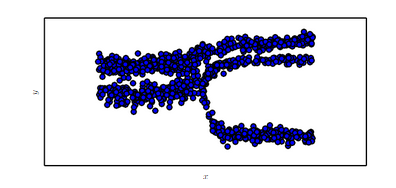
\includegraphics[width=6in]{fig/chap6/6_4.png} 
   \centering
   \caption{样例是用有一个混合密度输出层的神经网络画得。输入x从一个均匀分布中采样,输出y从$p_{\text{model}}(y \mid x)$中采样。神经网络能够学习从输入到输出分布的参数的非线性映射。这些参数涉及了概率,这个概率决定了三个混合部分中的哪个将产生输出和每个混合部分的参数。每个混合部分是有预测的均值和方差的高斯分布。输出分布的所有这些部分能依据输入$x$而变化,并且也在非线性方式中这样做。}
   \label{fig:6_4}
\end{figure}






%%%%%%%%%%%%%%%%%%%%%%%%%%%%%%%%%%%%%%%%%%%%%%%%%%%%%%%%%
%%%%%%%%%%%%%%%%%%% author:liviclee %%%%%%%%%%%%%%%%%%%%%
%%%%%%%%%%%%%%%%%%% part:6.3-6.7    %%%%%%%%%%%%%%%%%%%%%
%%%%%%%%%%%%%%%%%%%%%%%%%%%%%%%%%%%%%%%%%%%%%%%%%%%%%%%%%

\section{隐藏单元}
\label{sec:6.3}

\section{架构设计}
\label{sec:6.4}

\section{反向传播及其他微分算法}
\label{sec:6.5}

\section{前馈神经网络的发展史}
\label{sec:6.6}

\chapter{深度学习的正则化}
\label{chap:7}
%%%%%%%%%%%%%%%%%%%%%%%%%%%%%%%%%%%%%%%%%%%%%%%%%%%%%%%%%
%%%%%%%%%%%%%%%%%% author:ai0825 %%%%%%%%%%%%%%%%%%%%%%%%
%%%%%%%%%%%%%%%%%%%%%%%%%%%%%%%%%%%%%%%%%%%%%%%%%%%%%%%%%
\chapter{训练深度模型的优化方法}
\label{chap:8}
%%%%%%%%%%%%%%%%%%%%%%%%%%%%%%%%%%%%%%%%%%%%%%%%%%%%%%%%%
%%%%%%%%%%%%%%%%%%% author:wzwei1636@163.com  %%%%%%%%%%%
%%%%%%%%%%%%%%%%%%% part:8.0-8.2              %%%%%%%%%%%
%%%%%%%%%%%%%%%%%%%%%%%%%%%%%%%%%%%%%%%%%%%%%%%%%%%%%%%%%
\section{8.0}
%%%%%%%%%%%%%%%%%%%%%%%%%%%%%%%%%%%%%%%%%%%%%%%%%%%%%%%%%
%%%%%%%%%%%%%%%%%%% author:SilentSkyWalker %%%%%%%%%%%%%%
%%%%%%%%%%%%%%%%%%% part:8.3-8.5           %%%%%%%%%%%%%%
%%%%%%%%%%%%%%%%%%%%%%%%%%%%%%%%%%%%%%%%%%%%%%%%%%%%%%%%%

\section{8.3}
%%%%%%%%%%%%%%%%%%%%%%%%%%%%%%%%%%%%%%%%%%%%%%%%%%%%%%%%%
%%%%%%%%%%%%%%%%%%% author:dimitri0802 %%%%%%%%%%%%%%%%%%
%%%%%%%%%%%%%%%%%%% part:8.6-8.7       %%%%%%%%%%%%%%%%%%
%%%%%%%%%%%%%%%%%%%%%%%%%%%%%%%%%%%%%%%%%%%%%%%%%%%%%%%%%

\section{8.6}
\chapter{卷积网络}
\label{chap:9}
%%%%%%%%%%%%%%%%%%%%%%%%%%%%%%%%%%%%%%%%%%%%%%%%%%%%%%%%%
%%%%%%%%%%%%%%%%%%% author:ifighting %%%%%%%%%%%%%%%%%%%%
%%%%%%%%%%%%%%%%%%% part:9.1-9.6     %%%%%%%%%%%%%%%%%%%%
%%%%%%%%%%%%%%%%%%%%%%%%%%%%%%%%%%%%%%%%%%%%%%%%%%%%%%%%%

Convolutional Network,也叫做CNN,是一种专门用来处理具有类似网格拓补结构的数据的神经网络。
例如时间序列数据(可以认为是在时间轴上按照特定规律地采样形成的一维网格)和图像数据(可以看作是二维的由像素组成的网格)。
Convolutional network在很多应用领域都表现优秀。
Convolutional network一词说明这种网络使用了convolution这种数学运算。
卷积是一种特殊的线性运算。convolutional network是指那些至少在网络的一层中使用卷积运算来替代一般的矩阵乘法运算的神经网络。

本章,我们首先说明什么是卷积运算。
接着,我们会解释在神经网络中使用卷积运算的动机。
然后我们会介绍一种几乎所有的CNN都会用到的操作pooling。
通常来说,CNN中用到的卷积运算和其他领域(例如工程领域以及纯数学领域)中的定义并不完全一致。
我们会对神经网络实践中用得比较多的几种卷积函数的变体进行说明。
我们也会说明如何在多种不同维数的数据上使用卷积运算。
之后我们讨论使得卷积运算更加高效的一些方法。
CNN是神经科学的原理影响深度学习的典型代表,之后我们也会讨论这些神经科学的原理,并对卷积神经网络在深度学习发展史中的作用作出评价。
本章没有介绍如何为你的卷积神经网络选择合适的结构,因为本章的目标是描述CNN提供的强大工具,第11章会对在具体环境中使用相应的工具给出一些指导。
对于convolutional network结构的研究进展得如此迅速,以至于在特定的基准线上,数月甚至几周就会产生一个新的最优的网络结构,以至于评价究竟哪种结构是最好的也是不切实际的。然而,最好的网络结构也是由本章所描述的基本部件搭建起来的。

 
\section{卷积运算}

一般而言,卷积是对两个实值函数的一种数学运算。为了给出卷积的定义,我们从两个可能会用到的函数的例子出发。

假设我们正在使用激光传感器追踪一艘宇宙飞船的位置。我们的激光传感器给出一个单独的输出$x(t)$,表示宇宙飞船在时刻$t$ 的位置。$x$和$t$都是实值的,这意味着我们可以在任意的某个时刻从传感器中获取飞船的位置。

现在假设我们的传感器的输出含有噪声。为了减少噪声对飞船位置估计的影响,我们对得到的测量结果进行平均。
显然,时间上越近的测量结果越相关,因此我们采用一种加权平均的方法,对于越近的测量结果赋予更高的权值。
我们采用一个加权函数$w(a)$ 来实现,其中$a$表示测量结果据当前时刻的时间间隔。如果我们在任意时刻都采用这种加权平均的操作,就得到了对于飞船位置的连续估计函数$s$:
\begin{equation}
s(t) = \int x(a)w(t-a)da.
\end{equation}

这种运算就叫做(卷积)convolution。
卷积运算通常用星号表示:
\begin{equation}
s(t) = (x*w)(t).
\end{equation}

在我们的例子中,$w$必须是一个有效的概率密度函数,否则输出就不再是一个加权平均。
另外,$w$在参数为负值时必须为0,否则它会涉及到未来,这不是我们能够做到的。
但这些限制条件只是针对当前这个例子。
一般而言,卷积被定义在满足上述积分式的任意函数上,并且也可能被用于加权平均以外的目的。
在CNN的术语中,第一个参数(在这个例子中,函数$x$)叫做input,第二个参数(函数$w$)叫做kernel。
输出有时被称作feature map。 
在这个例子中,激光传感器给出连续的任意时刻测量结果的想法是不现实的。
一般而言,当我们用计算机处理数据时,时间会被离散化,传感器会给出特定时间间隔的数据。
所以比较现实的的假设是传感器每秒给出一次测量结果,这样,时间$t$只能取整数值。
如果我们假设$x$和$w$都定义在整数时刻$t$上,就得到了离散形式的卷积:

\begin{equation}
s(t) = (x*w)(t) = \sum_{a = -\infty}^{\infty} x(a)w(t-a).
\end{equation}

在机器学习的应用中,输入一般是高维矩阵数据,而kernal也是由算法产生的高维矩阵数据。
我们把这种高维矩阵数据叫做张量。
因为输入与核的每一个元素都分开存储,我们经常假设在存储了数据的有限点集以外,这些函数的值都为零。
这意味着在实际操作中,我们可以统一地把无限的求和当作对有限个数组元素的求和来用。
最后,我们有时对多个维度进行卷积运算。
例如,如果把二维的图像$I$作为输入,我们也相应的需要使用二维的核$K$:

\begin{equation}
S(i,j) = (I*K)(i,j) = \sum_m \sum_n I(m,n) K(i-m, j-n).
\end{equation}

卷积是具有交换性质(commutative),我们可以等价地写作:

\begin{equation}
S(i, j) = (K*I)(i,j) = \sum_m \sum_n I(i-m, j-n) K(m, n).
\end{equation}

通常,下面的公式在机器学习库中更方便应用,因为它在$m$和$n$的有效范围内变化更少。

 
卷积运算可交换性的出现是因为我们相对输入翻转了kernal,这意味着当$m$增大时,输入的索引增大,但核的索引相应的减小。
翻转核的唯一目的就是为了得到可交换性。
尽管可交换性在证明时很有用,但在神经网络的应用中却不是一个重要的性质。
与之不同的是,许多神经网络库会实现一个相关的函数,称为cross correlation,和卷积运算几乎一样但是并不翻转核:

\begin{equation}
S(i, j) = (I*K)(i, j) = \sum_m \sum_n I(i+m, j+n) K(m, n).
\end{equation}

许多机器学习的库使用互相关函数但是叫它卷积。
在这本书中我们遵循把两种运算都叫做卷积的这个传统,只有在用到核的翻转时才会在上下文中特别指明区别。
在机器学习中,学习算法会在核合适的位置学得恰当的值, 所以一个基于核翻转的卷积运算的学习算法所学得的核,是对未进行翻转的算法学得的核的翻转。
单独使用卷积运算在机器学习中是很少见的,卷积经常和其他的函数一起使用,无论卷积运算是否翻转了它的核,这些函数的组合通常是不可交换的。

图9.1演示了一个在2维张量上的卷积运算(核没有翻转)的例子。

%待补充插图

离散卷积可以看作矩阵的乘法,然而,这个矩阵的一些元素被限制为必须和另一些元素相等。
例如对于单变量的离散卷积,矩阵的每一行都必须和上一行移动一个元素后相等。
这种矩阵叫做Toeplitz matrix。
对于二维情况,卷积对应着一个doubly block circulant matrix(二维矩阵)。
除了这些元素相等的限制以外,卷积通常对应着一个非常稀疏的矩阵(几乎所有的元素都为零)。
这是因为核通常要远小于输入的图像。任何一个使用矩阵乘法但是并不依赖矩阵结构的特殊性质的神经网络算法,都适用于卷积运算,并且不需要对神经网络做出大的修改。
典型的CNN为了更有效地处理大规模输入,确实使用了一些专门化的技巧,但这些在理论分析方面并不是严格必要的。

 
\section{动机}

卷积运算通过三个重要的思想来帮助改进机器学习系统:sparse interactions(局部感知)、parameter sharing(权值共享)、equivariant representations。
另外,卷积提供了一种处理大小可变的输入的方法。我们会在下文中依次介绍这些思想。

传统的神经网络使用矩阵乘法来建立输入与输出的连接关系。
其中,参数矩阵的每一个独立的参数都描述了每一个输入单元与每一个输出单元间的交互。
这意味着每一个输出单元与每一个输入单元都产生交互。
然而,CNN具有sparse interactions(也叫做sparse connectivity或者sparse weights)的特征。
这通过使得核的规模远小于输入的规模来实现。
举个例子,当进行图像处理时,输入的图像可能包含百万个像素点,但是我们可以通过只占用几十到上百个像素点的核来探测一些小的有意义的特征,例如图像的边缘。
这意味着我们需要存储的参数更少,不仅减少了模型的存储需求,而且提高了它的统计效率。
这也意味着为了得到输出我们只需要更少的计算量。
这些效率上的提高往往是很显著的。
如果有$m$个输入和$n$个输出,那么矩阵乘法需要$m \times n$个参数并且相应算法的时间复杂度为$O(m\times n)$(对于每一个例子)。
如果我们限制每一个输出拥有的连接数为$k$,那么稀疏的连接方法只需要$k\times n$个参数以及$O(k\times n)$的运行时间。
在很多应用方面,只需保持$k$的数量级远小于$m$,就能在机器学习的任务中取得好的表现。
sparse connectivity(局部感知)的图形化解释如图\ref{fig:chap9_area_of_effect}和图\ref{fig:chap9_receptive_field}所示。
在深度卷积网络中,处在深层的单元可能不直接地与绝大部分输入连接,如图\ref{fig:chap9_deep_receptive_field}所示。
这允许网络可以通过只描述sparse interactions的区域来高效地描述多个变量的复杂交互过程。


% fig 9.2
\begin{figure}[!htb]
\ifOpenSource
\centerline{\includegraphics{figure.pdf}}
\else
\centerline{\includegraphics{Chapter9/figures/area_of_effect}}
\fi
\captionsetup{singlelinecheck=off}
\caption[Caption for LOF]{\gls{sparse_connectivity},对每幅图从下往上看。我们强调了一个输入单元$x_3$以及在$\bm{s}$中受该单元影响的输出单元。\emph{(上)}当$\bm{s}$是由核宽度为3的卷积产生时,只有三个输出受到$\bm{x}$的影响\protect\footnotemark。\emph{(下)}当$\bm{s}$是由矩阵乘法产生时,连接不再是稀疏的,所以所有的输出都会受到$x_3$的影响。}
\label{fig:chap9_area_of_effect}
\end{figure}
 \footnotetext{译者注:译者认为此处应当是$x_3$。}
% fig 9.3
\begin{figure}[!htb]
\ifOpenSource
\centerline{\includegraphics{figure.pdf}}
\else
\centerline{\includegraphics{Chapter9/figures/receptive_field}}
\fi
\captionsetup{singlelinecheck=off}
\caption[.]{\gls{sparse_connectivity},对每幅图从上往下看。我们强调了一个输出单元$s_3$以及$\bm{x}$中影响该单元的输入单元。这些单元被称为$s_3$的\gls{receptive_field}。\emph{(上)}当$\bm{s}$是由核宽度为3的卷积产生时,只有三个输入影响$s_3$。\emph{(下)}当$\bm{s}$是由矩阵乘法产生时,连接不再是稀疏的,所以所有的输入都会影响$s_3$。}


\label{fig:chap9_receptive_field}
\end{figure}
% fig 9.4
\begin{figure}[!htb]
\ifOpenSource
\centerline{\includegraphics{figure.pdf}}
\else
\centerline{\includegraphics{Chapter9/figures/deep_receptive_field}}
\fi
\caption{处于\gls{convolutional_network}更深的层中的单元,它们的\gls{receptive_field}要比处在浅层的单元的\gls{receptive_field}更大。如果网络还包含类似\gls{stride}卷积(图\ref{fig:chap9_stride_conv})或者\gls{pooling}(\ref{sec:pooling}节)之类的结构特征,这种效应会加强。这意味着在\gls{convolutional_network}中即使是\emph{直接}连接都是很稀疏的,处在更深的层中的单元可以\emph{间接地}连接到全部或者大部分输入图像。}
\label{fig:chap9_deep_receptive_field}
\end{figure}

 
\firstgls{parameter_sharing}是指在一个模型的多个函数中使用相同的参数。
在传统的神经网络中,当计算一层的输出时,权值矩阵的每一个元素只使用一次,当它乘以输入的一个元素后就再也不会用到了。
作为\gls{parameter_sharing}的同义词,我们可以说一个网络含有\firstgls{tied_weights},因为用于一个输入的权值也会被绑定在其他的权值上。
在\gls{CNN}中,核的每一个元素都作用在输入的每一位置上(除了一些可能的边界像素,取决于对于边界的决策设计)。
卷积运算中的\gls{parameter_sharing}保证了我们只需要学习一个参数集合,而不是对于每一位置都需要学习一个单独的参数集合。
这虽然没有改变前向传播的时间(仍然是$O(k\times n)$),但它显著地把模型的存储需求降低至$k$个参数,并且$k$通常是远小于$m$的数量级。
因为$m$ 和$n$通常规模很接近,$k$在实际中相对于$m\times n$是很小的。
因此,卷积在存储需求和统计效率方面极大地优于稠密矩阵的乘法运算。
图\ref{fig:chap9_parameter_sharing}演示了\gls{parameter_sharing}是如何实现的。
% fig 9.5
\begin{figure}[!htb]
\ifOpenSource
\centerline{\includegraphics{figure.pdf}}
\else
\centerline{\includegraphics{Chapter9/figures/parameter_sharing}}
\fi
\caption{\gls{parameter_sharing}。黑色箭头表示在两个不同的模型中使用了特殊参数的连接。\emph{(上)}黑色箭头表示在卷积模型中3元素核的中间元素的使用。因为\gls{parameter_sharing},这单个参数被用于所有的输入位置。\emph{(下)}这单个黑色箭头表示在全连接模型中权重矩阵的中间元素的使用。这个模型没有使用\gls{parameter_sharing},所以参数只使用了一次。}
\label{fig:chap9_parameter_sharing}
\end{figure}
% -- 326 --
 
% -- 327 --
 
作为前两条原则的一个实际例子,图\ref{fig:chap9_efficiency_of_edge_detection}说明了\gls{sparse_connectivity}和\gls{parameter_sharing}是如何显著地提高用于图像边缘检测的线性函数的效率的。
% fig 9.6
\begin{figure}
\ifOpenSource
\centerline{\includegraphics{figure.pdf}}
\else
\centering    
\subfigure{ \label{fig:chap9_efficiency_of_edge_detection_a}     
\includegraphics[width=0.35\textwidth]{Chapter9/figures/sundance.png}}     
\subfigure{ \label{fig:chap9_efficiency_of_edge_detection_b}     
\includegraphics[width=0.35\textwidth]{Chapter9/figures/edges.png}}     
\fi
\captionsetup{singlelinecheck=off}
\caption{边缘检测的效率。右边的图像是通过获得原始图像中的每个像素并减去左边相邻像素的值而形成的。这给出了输入图像中所有垂直方向上的边缘的强度,这对目标检测是有用的操作。两个图像都是280像素的高度。输入图像宽320像素,而输出图像宽319像素。这个变换可以通过包含两个元素的卷积核来描述,并且需要$319\times 280\times 3 = 267,960$个浮点运算(每个输出像素需要两次乘法和一次加法)。为了用矩阵乘法描述相同的变换,需要$320\times 280\times 319\times 280$个或者说超过80亿个元素的矩阵,这使得卷积对于表示这种变换更有效40亿倍。直接运行矩阵乘法的算法将执行超过160亿个浮点运算,这使得卷积在计算上大约有60,000倍的效率。当然,矩阵的大多数元素将为零。如果我们只存储矩阵的非零元,则矩阵乘法和卷积都需要相同数量的浮点运算来计算。矩阵仍然需要包含$2\times 319\times 280=178,640$个元素。将小的局部区域上的相同线性变换应用到整个输入上,卷积是描述这种变换的极其有效的方法。照片来源:Paula Goodfellow。}   
\label{fig:chap9_efficiency_of_edge_detection}     
\end{figure}
 
对于卷积,权值的特殊形式使得神经网络层具有平移不变性。
如果一个函数满足输入改变,输出也以同样的方式改变这一性质,我们就说它是等变(equivariant)的。
特别地,如果函数$f(x)$与$g(x)$满足$f(g(x))= g(f(x))$,我们就说$f(x)$对于变换$g$具有等变性。
对于卷积来说,如果令$g$是任意的输入平移函数,那么卷积函数对于$g$具有等变性。
举个例子,令$I$表示图像的明亮度函数(取值为整数),$g$表示图像函数的变换函数(把一个图像函数映射到另一个图像函数的函数)使得$I' = g(I)$,其中$I'(x,y) = I(x-1, y)$。
这个函数把$I$中的每个像素向右移动一格。
如果我们先对$I$进行这种变换然后进行卷积操作所得到的结果,与先对$I$进行卷积然后再对输出使用平移函数$g$得到的结果是一样的。
当处理时间序列数据时,卷积产生一条用来表明输入中出现不同特征的某种时间轴。
如果我们把输入中的一个事件向后延时,在输出中也会有完全相同的表示,只是时间延时了。
图像与之类似,卷积产生了一个2维映射来表明某种属性在输入的什么位置出现了。
如果我们移动输入中的对象,它的表示也会在输出中移动同样的量。
当处理多个输入位置时,一些作用在邻居像素的函数是很有用的。
例如在处理图像时,在CNN的第一层进行图像的边缘检测是很有用的。
相同的边缘或多或少地散落在图像的各处,所以应当对整个图像有权值共享
但在某些情况下,我们并不希望对整幅图共享权值。
例如当我们在处理人脸图像(图像已经被剪裁成人脸在中心)时,我们可能会希望在不同的部位探测出不同的特征(处理人脸上部的网络需要去搜寻眉毛,处理人脸下部的网络就需要去搜寻下巴了)。

 
卷积对其他的一些变换并不是天然等变的,例如对于图像尺度或者角度的变换,需要其他的一些机制来处理这些变换。

最后,一些不能被传统的由(固定大小的)矩阵乘法定义的神经网络处理的特殊数据,可能通过卷积神经网络来处理,我们将在\ref{sec:data_types}节中进行讨论。

\section{pooling}

卷积神经网络的卷积层通常包含三级(如图\ref{fig:chap9_conv_layer}所示)。
在第一级中,卷积层并行地进行多个卷积运算来产生一组线性激活函数。
在第二级中,非线性的激活函数如ReLU函数等作用在第一级中的每一个线性输出上。
这一级有时也被称为detector stage(检测阶段?)。
在第三级中,我们使用pooling funciton函数(下采样函数)来更进一步地调整卷积层的输出。


% fig 9.7
\begin{figure}[!htb]
\ifOpenSource
\centerline{\includegraphics{figure.pdf}}
\else
\centerline{\includegraphics{Chapter9/figures/conv_layer}}
\fi
\caption{典型\gls{CNN}层的组件。有两组常用的术语用于描述这些层。\emph{(左)}在这组术语中,\gls{convolutional_network}被视为少量相对复杂的层,每层具有许多``级''。在这组术语中,核张量与网络层之间存在一一对应关系。在本书中,我们通常使用这组术语。\emph{(右)}在这组术语中,\gls{convolutional_network}被视为更大数量的简单层;每一个处理步骤都被认为是一个独立的层。这意味着不是每个``层''都有参数。}
\label{fig:chap9_conv_layer}
\end{figure}

pooling函数(下采样层)使用某一位置的相邻输出的总体统计特征来代替网络在该位置的输出。
例如,max pooling函数给出相邻矩形区域内的最大值。
其他常用的pooling函数包括相邻矩形区域内的平均值、$L^2$范数以及依靠据中心像素距离的加权平均函数。

 
不管采用什么样的pooling函数,当输入作出少量平移时,pooling能帮助我们的表示近似不变的。
对于平移的不变性是说当我们把输入平移一微小的量,大多数通过pooling函数的输出值并不会发生改变。
图\ref{fig:chap9_max_pool_invariance}用了一个例子来说明这是如何实现的。
局部平移不变性是一个很重要的性质,尤其是当我们关心某个特征是否出现而不关心它出现的具体位置时。
例如,当判定一张图像中是否包含人脸时,我们并不需要知道眼睛的具体像素位置,我们只需要知道有一只眼睛在脸的左边,有一只在右边就行了。
但在一些其他领域,保存特征的具体位置却很重要。
例如当我们想要寻找一个由两条边相交而成的拐角时,我们就需要很好地保存边的位置来判定它们是否相交。

% fig 9.8
\begin{figure}[!htb]
\ifOpenSource
\centerline{\includegraphics{figure.pdf}}
\else
\centerline{\includegraphics{Chapter9/figures/max_pool_invariance}}
\fi
\caption{\gls{max_pooling}引入不变性。\emph{(上)}卷积层中间输出的视图。下面一行显示非线性的输出。上面一行显示\gls{max_pooling}的输出,每个\gls{pool}的宽度为三个像素并且\gls{pooling}区域的\gls{stride}为一个像素。\emph{(下)}相同网络的视图,不过对输入右移了一个像素。下面一行的所有值都发生了改变,但上面一行只有一半的值发生了改变,这是因为\gls{max_pooling}单元只对周围的最大值比较敏感,而不是对精确的位置。}
\label{fig:chap9_max_pool_invariance}
\end{figure}

 
使用pooling可以认为网络结构中增加了一个无限强的先验:卷积层学得的函数必须具有对少量平移的不变性。当这个假设成立时,pooling可以极大地提高网络的统计效率。

pooling对于空间区域具有平移不变性,但当我们对于分离参数的卷积输出进行pooling操作时,特征能够学得应该对于哪种变换具有不变性(如图\ref{fig:chap9_learned_rotation}所示)。


% fig 9.9
\begin{figure}[!htb]
\ifOpenSource
\centerline{\includegraphics{figure.pdf}}
\else
\centerline{\includegraphics{Chapter9/figures/learned_rotation}}
\fi
\caption{学习不变性的示例。使用分离的参数学得多个特征,再使用\gls{pooling}单元进行\gls{pooling},可以学得对输入的某些变换的不变性。这里我们展示了用三个学得的过滤器和一个\gls{max_pooling}单元可以学得对旋转变换的不变性。这三个过滤器都旨在检测手写的数字5。每个过滤器尝试匹配稍微不同方向的5。当输入中出现5时,相应的过滤器会匹配它并且在探测单元中引起大的激活。然后,无论哪个探测单元被激活,\gls{max_pooling}单元都具有大的激活。我们在这里展示网络如何处理两个不同的输入,导致两个不同的探测单元被激活。然而对\gls{pooling}单元的影响大致相同。这个原则在\gls{maxout}网络\citep{Goodfellow-et-al-ICML2013}和其他卷积网络中使用。空间位置上的\gls{max_pooling}对于平移是天然不变的;这种多通道方法只在学习其他变换时是必要的。}
\label{fig:chap9_learned_rotation}
\end{figure}

 
因为pooling总结了全部的周围邻居的反馈,这使得pooling单元少于探测单元成为可能,我们可以通过综合pooling区域的$k$个像素的统计特征而不是单个像素来实现。
图\ref{fig:chap9_pool_downsample}给出了一个例子。
这种方法提高了网络的计算效率,因为下一层少了约$k$ 倍的输入。
当下一层的参数数目是其输入大小的函数时(例如当下一层是全连接的依赖矩阵乘法的网络层时),这种对于输入规模的减小也可以提高统计效率并且减少对于参数的存储需求。


% fig 9.10
\begin{figure}[!htb]
\ifOpenSource
\centerline{\includegraphics{figure.pdf}}
\else
\centerline{\includegraphics{Chapter9/figures/pool_downsample}}
\fi
\caption{带有\gls{downsampling}的\gls{pooling}。这里我们使用\gls{max_pooling},\gls{pool}的宽度为三并且\gls{pool}之间的\gls{stride}为二。这使得表示的大小减少了一半,减轻了下一层的计算和统计负担。注意到最右边的\gls{pooling}区域尺寸较小,但如果我们不想忽略一些探测单元的话就必须包含这个区域。}
\label{fig:chap9_pool_downsample}
\end{figure}

 
在很多任务中,pooling对于处理不同大小的输入具有重要作用。
例如我们想对不同大小的图像进行分类时,分类层的输入必须是固定的大小,而这通常通过调整pooling区域的偏置大小来实现,这样分类层总是能接收到相同数量的统计特征而不管最初的输入大小了。
例如,最终的pooling层可能会输出四组综合统计特征,每组对应着图像的一个象限,而与图像的大小无关。

一些理论工作对于在不同情况下应当使用哪种pooling函数给出了一些指导。
动态地把特征pooling在一起也是可行的,例如,通过针对具有特定性质的位置运行聚类算法。
这种方法对于每幅图像产生一个不同的pooling区域集合。
另一种方法是先学习一个单独的pooling结构,再应用到全部的图像中。

pooling可能会使得一些利用自顶向下信息的神经网络结构变得复杂,例如玻尔兹曼机和稀疏自编码器。
这些问题将在第\ref{part:deep_learning_research}部分中当我们遇到这些类型的网络时进一步讨论。
convolutional Boltzmann machines 中的\gls{pooling}出现在\ref{sec:convolutional_boltzmann_machines}节。
一些可微网络中需要的在{pooling单元中进行的类逆运算将在\ref{sec:convolutional_generative_networks}节中讨论。

图\ref{fig:chap9_cnn_classifier}给出了一些使用卷积和\gls{pooling}操作的用于分类的\gls{CNN}的完整结构的例子。
% fig 9.11
\begin{figure}[!htb]
\ifOpenSource
\centerline{\includegraphics{figure.pdf}}
\else
\centerline{\includegraphics{Chapter9/figures/cnn_classifier}}
\fi
\caption{\gls{convolutional_network}用于分类的架构示例。本图中使用的具体\gls{stride}和深度并不适合实际使用;它们被设计得非常浅以适合页面。实际的\gls{convolutional_network}也常常涉及大量的分支,不同于这里为简单起见所使用的链式结构。\emph{(左)}处理固定大小的图像的\gls{convolutional_network}。在卷积层和\gls{pooling}层几层交替之后,卷积特征映射的张量被重新整形以展平空间维度。网络的其余部分是一个普通的前馈网络分类器,如第\ref{chap:deep_feedforward_networks}章所述。\emph{(中)}处理大小可变的图像的\gls{convolutional_network},但仍保持全连接的部分。该网络使用具有可变大小但是数量固定的\gls{pool}的\gls{pooling}操作,以便向网络的全连接部分提供576个单位的固定大小的向量。 \emph{(右)}没有任何全连接权重层的\gls{convolutional_network}。相反,最后的卷积层为每个类输出一个特征映射。该模型可能学习每个类在每个空间位置出现的可能性的映射。将特征映射进行平均得到的单个值,提供了顶部softmax分类器的变量。}
\label{fig:chap9_cnn_classifier}
\end{figure}

\section{卷积与\glsentrytext{pooling}作为一种无限强的先验}


回忆一下\ref{sec:capacity_overfitting_and_underfitting}节中prior probability distribution(先验概率分布)的概念。

这是一个模型参数的概率分布,它表示在我们了解数据之前我们假设数据是处于什么分布。

 
先验被认为是强或者弱取决于先验中概率密度的集中程度。
弱先验具有较高的熵值,例如方差很大的gaussian distribution,这样的先验允许数据对于参数的改变具有或多或少的自由性。
强先验具有较低的熵值,例如方差很小的gaussian distribution,这样的先验在决定参数最终取值时起着更加积极的作用。

一个无限强的先验对一些参数的概率置零并且要求禁止对这些参数赋值,无论数据对于这些参数的值给出了多大的支持。

我们可以把CNN想成和全连接网络类似,但对于这个全连接网络的权值有一个无限强的先验。
这个无限强的先验是说一个隐藏神经元的权值必须和它邻居的权值相等,但在空间中改变。
这个先验也要求除了那些处在神经元空间连续的小的接收域以内的权值外,其余的权值都为零。

总之,我们可以把卷积的使用当作是对网络中一层的参数引入了一个无限强的先验概率分布。
这个先验是说该层应该学得的函数只包含局部连接关系并且对平移具有等变性。
类似的,使用下采样层也是一个无限强的先验:每一个单元都具有对少量平移的不变性。

当然,把CNN当作一个具有无限强先验的全连接网络来实现会导致极大的计算浪费。
但把CNN想成具有无限强先验的全连接网络可以帮助我们更好地理解CNN是如何工作的。

其中一个关键的地方是卷积和pooling可能导致欠拟合。
与任何其他先验类似,卷积和pooling只有当先验的假设合理且正确时才有用。

如果一项任务依赖于保存精确的空间信息,那么在所有的特征上使用pooling将会增大训练误差。
一些CNN\citep{Szegedy-et-al-arxiv2014}为了既获得具有较高不变性的特征又获得当平移不变性不合理时不会导致欠拟合的特征,被设计成在一些通道上使用\gls{pooling}而在另一些通道上不使用。
当一项任务涉及到要对输入中相隔较远的信息进行合并时,那么卷积所需要的先验可能就不正确了。

另一个关键洞察是当我们比较卷积模型的统计学习表现时,只能以基准中的其他卷积模型作为比较的对象。
其他不使用卷积的模型即使我们把图像中的所有像素点都置换后依然有可能进行学习。
对于许多图像数据集,还有一些分别的基准,有些是针对那些具有\firstgls{permutation_invariant}并且必须通过学习发现拓扑结构的模型,还有一些是针对设计者将空间关系的知识通过硬编码给了它们的模型。

% -- 336 --

\section{基本卷积函数的变体}
\label{sec:variants_of_the_basic_convolution_function}

当在神经网络的上下文中讨论卷积时,我们通常不是特指数学文献中使用的那种标准的离散卷积运算。
实际应用中的函数略微有些不同。
这里我们详细讨论一下这些差异,并且对神经网络中用到的函数的一些重要性质进行重点说明。

首先,当我们提到神经网络中的卷积时,我们通常是指一次特定的运算,而这种运算包含了并行地使用多个卷积。
这是因为带有单个核的卷积只能提取一种类型的特征,尽管它作用在多个空间位置上。
我们通常希望神经网络的一层能够在多个位置提取多种类型的特征。

另外,输入通常也不仅仅是实值的网格,而是由一系列向量值的观测数据构成的网格。
例如,一幅彩色图像在每一个像素点都会有红绿蓝三种颜色的亮度。
在多层的CNN中,第二层的输入是第一层的输出,通常在每个位置包含多个卷积的输出。
当用于图像时,我们通常把卷积的输入输出都看作是3维的张量,其中一个索引用于标明不同的通道(例如红绿蓝),另外两个索引标明在每个通道上的空间坐标。
软件实现通常使用批处理模式,所以它们会使用4维的张量,第四维索引用于标明批处理中不同的实例,但我们为简明起见这里忽略批处理索引。

因为CNN通常使用多通道的卷积,它们基于的线性运算并不保证一定是可交换的,即使使用了核翻转也是如此。
这些多通道的运算只有当其中的每个运算的输出和输入具有相同的通道数时才是可交换的。

假定我们有一个4维的核张量$\TSK$,它的每一个元素是$\TEK_{i,j,k,l}$,表示输出的处于通道$i$中的一个单元和输入的处于通道$j$中的一个单元的连接强度,并且在输出单元和输入单元之间有一个$k$行$l$列的偏置。

假定我们的输入由观测数据$\TSV$组成,它的每一个元素是$\TEV_{i,j,k}$,表示处在通道$i$中第$j$行第$k$列的值。

假定我们的输出$\TSZ$和输入$\TSV$具有相同的形式。如果输出$\TSZ$是通过对$\TSK$和$\TSV$进行卷积而不涉及翻转$\TSK$得到的,那么

\begin{equation}
\TEZ_{i,j,k} = \sum_{l,m,n} \TEV_{l, j+m-1, k+n-1} \TEK_{i,l,m,n},
\end{equation}

这里对所有的$l$,$m$和$n$进行求和是对所有(在求和式中)有效的张量索引的值进行求和。
在线性代数中,向量的索引通常从1开始,这就是上述公式中$-1$的由来。
但是像C或Python这类编程语言索引通常从0开始,这使得上述公式可以更加简洁。

 
我们有时会希望跳过核中的一些位置来降低计算的开销(相应的代价是提取特征没有先前那么好了)。
我们可以把这一过程看作是对卷积函数输出的下采样(downsampling)。
如果我们只想对输出的每个方向上的$s$个像素进行采样,那么我们可以定义一个下采样卷积函数$c$使得
\begin{equation}
\TEZ_{i,j,k} = c(\TSK, \TSV, s)_{i,j,k} = \sum_{l,m,n} [\TEV_{l,(j-1)\times s+m, (k-1)\times s +n,}
 \TEK_{i,l,m,n}].
 \label{eq:9.8}
\end{equation}
我们把$s$称为下采样卷积的stride(步长)。
当然也可以对每个移动方向定义不同的步幅。
图\ref{fig:chap9_stride_conv}演示了一个实例。
% fig 9.12
\begin{figure}[!htb]
\ifOpenSource
\centerline{\includegraphics{figure.pdf}}
\else
\centerline{\includegraphics{Chapter9/figures/stride_conv}}
\fi
\caption{带有\gls{stride}的卷积。在这个例子中,我们的\gls{stride}为二。\emph{(上)}在单个操作中实现的\gls{stride}为二的卷积。\emph{(下)}\gls{stride}大于一个像素的卷积在数学上等价于单位\gls{stride}的卷积随后\gls{downsampling}。显然,涉及\gls{downsampling}的两步法在计算上是浪费的,因为它计算了许多将被丢弃的值。}
\label{fig:chap9_stride_conv}
\end{figure}

在任何CNN的应用中都有一个重要性质,那就是能够隐含地对输入$\TSV$用零进行填充(pad)使得它加宽。
如果没有这个性质,表示的宽度在每一层就会缩减,缩减的幅度是比核少一个像素这么多。
对输入进行零填充允许我们对核的宽度和输出的大小进行独立的控制。
如果没有零填充,我们就被迫面临二选一的局面,要么选择网络空间宽度的快速缩减,要么选择一个小型的核——这两种情境都会极大得限制网络的表示能力。

图\ref{fig:chap9_zero_pad_shrink}给出了一个例子。
% fig 9.13
\begin{figure}[!htb]
\ifOpenSource
\centerline{\includegraphics{figure.pdf}}
\else
\centerline{\includegraphics{Chapter9/figures/zero_pad_shrink}}
\fi
\caption{零填充对网络大小的影响。考虑一个\gls{convolutional_network},每层有一个宽度为六的核。 在这个例子中,我们不使用任何\gls{pooling},所以只有卷积操作本身缩小网络的大小。\emph{(上)}在这个卷积网络中,我们不使用任何隐含的零填充。这使得表示在每层缩小五个像素。从十六个像素的输入开始,我们只能有三个卷积层,并且最后一层不能移动核,所以可以说只有两层是真正的卷积层。可以通过使用较小的核来减缓收缩速率,但是较小的核表示能力不足,并且在这种结构中一些收缩是不可避免的。\emph{(下)}通过向每层添加五个隐含的零,我们防止了表示随深度收缩。这允许我们设计一个任意深的卷积网络。}
\label{fig:chap9_zero_pad_shrink}
\end{figure}

有三种零填充设定的情况值得注意。
第一种是无论怎样都不使用零填充的极端情况,并且卷积核只允许访问那些图像中能够完全包含整个核的位置。
在MATLAB中,这称为valid卷积。

在这种情况下,输出的所有像素都是输入中相同数量像素的函数,这使得输出像素的表示更加规范。
然而,输出的大小在每一层都会缩减。
如果输入的图像宽度是$m$,核的宽度是$k$,那么输出的宽度就会变成$m-k+1$。
如果卷积核非常大的话缩减率会非常显著。
因为缩减数大于0,这限制了网络中能够包含的卷积层的层数。
当层数增加时,网络的空间维度最终会缩减到$1\times 1$,这种情况下另外的层就不可能进行有意义的卷积了。
第二种特殊的情况是只进行足够的零填充来保持输出和输入具有相同的大小
。
在MATLAB中,这称为same卷积。
在这种情况下,网络能够包含任意多的卷积层,只要硬件可以支持,这是因为卷积运算并没有改变相关的结构。
然而,输入像素中靠近边界的部分相比于中间部分对于输出像素的影响更小。
这可能会导致边界像素存在一定程度的欠表示。
这使得第三种极端情况产生了,在MATLAB中称为full卷积。

它进行了足够多的零填充使得每个像素在每个方向上恰好被访问了$k$次
这将导致学得一个在卷积特征映射的所有位置都表现不错的单核更为困难。
通常零填充的最优数量(对于测试集的分类正确率)处于``valid卷积''和``same卷积''之间的某个位置。



在一些情况下,我们并不一定真正想用卷积,而只是用一些局部连接的网络层。
在这种情况下,我们的多层感知机对应的邻接矩阵是相同的,但每一个连接都有它自己的权重,用一个6维的张量$\TSW$来表示。
$\TSW$的索引分别是:输出的通道$i$,输出的行$j$和列$k$,输入的通道$l$,输入的行偏置$m$和列偏置$n$。
局部连接层的线性部分可以表示为

\begin{equation}
\TEZ_{i,j,k} = \sum_{l,m,n} [\TEV_{l, j+m-1, k+n-1} w_{i, j, k, l, m, n}]. %这里应该是$\TEW$?,不清楚,待考证
\end{equation}
这有时也被称为unshared convolution(非权值共享的卷积?),因为它和带有一个小核的离散卷积运算很像,但并不横跨位置来共享参数。
图\ref{fig:chap9_local}比较了局部连接、卷积和全连接的区别。


% fig 9.14
\begin{figure}[!htb]
\ifOpenSource
\centerline{\includegraphics{figure.pdf}}
\else
\centerline{\includegraphics{Chapter9/figures/local}}
\fi
\caption{局部连接,卷积和全连接的比较。\emph{(上)}每一小片(接受域)有两个像素的局部连接层。每条边用唯一的字母标记,来显示每条边都有自身的权重参数。\emph{(中)}核宽度为两个像素的卷积层。该模型与局部连接层具有完全相同的连接。区别不在于哪些单元相互交互,而在于如何共享参数。局部连接层没有\gls{parameter_sharing}。卷积层在整个输入上重复使用相同的两个权重,正如用于标记每条边的字母重复出现所指示的那样。\emph{(下)}全连接层类似于局部连接层,它的每条边都有其自身的参数(在该图中用字母明确标记的话就太多了)。 然而,它不具有局部连接层的连接受限的特征。}
\label{fig:chap9_local}
\end{figure}
 

 
当我们知道每一个特征都是一小部分空间的函数而不是整个空间的特征时,局部连接层是很有用的。
例如,如果我们想要辨别一张图片是否是人脸图像时,我们只需要去寻找嘴是否在图像的下部中央部分即可。

使用那些连接被更进一步限制的卷积或者局部连接层也是有用的,例如,限制每一个输出的通道$i$仅仅是输入通道$l$的一部分的函数时。
实现这种情况的一种通用方法是使输出的前$m$个通道仅仅连接到输入的前$n$个通道,输出的接下来的$m$个通道仅仅连接到输入的接下来的$n$个通道,以此类推。


图\ref{fig:chap9_conv_groups}给出了一个例子。
对少量通道间的连接进行建模允许网络使用更少的参数,这降低了存储的消耗以及提高了统计效率,并且减少了前向和反向传播所需要的计算量。
这些目标的实现并没有减少隐藏神经元的数目。


% fig 9.15
\begin{figure}[!htb]
\ifOpenSource
\centerline{\includegraphics{figure.pdf}}
\else
\centerline{\includegraphics{Chapter9/figures/conv_groups}}
\fi
\caption{\gls{convolutional_network}的前两个输出通道只和前两个输入通道相连,随后的两个输出通道只和随后的两个输入通道相连。}
\label{fig:chap9_conv_groups}
\end{figure}

tiled convolution对卷积层和局部连接层进行了折衷。
这里并不是对每一个空间位置的权重集合进行学习,我们学习一组核使得当我们在空间移动时它们可以循环利用。
这意味着在近邻的位置上拥有不同的过滤器,就像局部连接层一样,但是对于这些参数的存储需求仅仅会增长常数倍,这个常数就是核的集合的大小,而不是整个输出的特征映射的大小。


图\ref{fig:chap9_tiled}对局部连接层、tiled convolution和标准卷积进行了比较。
% fig 9.16
\begin{figure}[!htb]
\ifOpenSource
\centerline{\includegraphics{figure.pdf}}
\else
\centerline{\includegraphics{Chapter9/figures/tiled}}
\fi
\captionsetup{singlelinecheck=off}
\caption[.]{局部连接层、\gls{tiled_convolution}和标准卷积的比较。当使用大小相同的核时,这三种方法的单元之间具有相同的连接。此图是对使用两个像素宽的核的说明。这三种方法之间的区别在于它们如何共享参数。\emph{(上)}局部连接层根本没有共享参数。我们对每个连接使用唯一的字母标记,来表明每个连接都有它自身的权重。\emph{(中)}\gls{tiled_convolution}有$t$个不同的核。这里我们说明$t=2$的情况。其中一个核具有标记为``a''和``b''的边,而另一个具有标记为``c''和``d''的边。我们每次在输出中向右移动一个像素,移动后使用不同的核。这意味着,与局部连接层类似,输出中的相邻单元具有不同的参数。与局部连接层不同的是,在我们遍历所有可用的$t$个核之后,我们循环回到了第一个核。如果两个输出单元间隔$t$个步长的倍数,则它们共享参数。\emph{(下)}传统卷积等效于$t=1$的\gls{tiled_convolution}。它只有一个核,并且被应用到各个地方,我们在图中表示为在各处使用具有标记为``a''和``b''的边的核。}
\label{fig:chap9_tiled}
\end{figure}
 

 
为了代数地定义tiled convolution},令$\TSK$是一个6维的张量
我们这里并不是使用分别的索引来表示输出映射中的每一个位置,输出的位置在每个方向上在$t$个不同的核的组成的集合中进行循环。
如果$t$等于输出的宽度,这就是局部连接层了。

\begin{equation}
\TEZ_{i, j, k} = \sum_{l, m, n} \TEV_{l, j+m-1, k+n-1} \TEK_{i, l, m, n, j\% t +1, k\% t+1},
\end{equation}
这里百分号是取模运算,其中$t\% t =0, (t+1)\% t = 1$等等。
在每一维上使用不同的$t$可以很直观地对这个公式进行扩展。
 

 
局部连接层与tiled convolution层都和max pooling有一些关联:这些层的探测单元都是由不同的滤波器产生的。
如果这些过滤器能够学会探测相同隐含特征的不同变换形式,那么max_pooling的单元对于学得的变换就具有不变性(如图\ref{fig:chap9_learned_rotation}所示)。
卷积层对于平移具有内置的不变性。
 

 
实现CNN时,采用除卷积以外一般要进行其他的操作。
为了实现学习,必须在给定输出的梯度时能够计算核的梯度。
在一些简单情况下,这种运算可以通过卷积来实现,但在很多我们感兴趣的情况下,包括stride大于1的情况,并不具有这样的性质。

由于卷积是一种线性运算,所以可以表示成矩阵乘法的形式(如果我们首先把输入张量变形为一个扁平的向量)。涉及到的矩阵是卷积核的函数。
这个矩阵是稀疏的并且核的每个元素都复制给矩阵的很多个元素。
这种观点能够帮助我们导出CNN需要的很多其他运算。

通过卷积定义的矩阵转置的乘法就是这样一种运算。
这种运算用于通过卷积层反向传播误差的导数,所以它在训练多于一个隐藏层的CNN时是必要的。
如果我们想要从隐藏层单元重构可视化单元时,同样的运算也是需要的。
重构可视化单元是本书第\ref{part:deep_learning_research}部分的模型广泛用到的一种运算,这些模型包括稀疏自编码器,限制玻尔兹曼机和稀疏编码等等。


构建这些模型的卷积化的版本都要用到转置化卷积。
就像核梯度的运算,这种输入梯度运算在某些情况下可以用卷积来实现,但在一般情况下需要用到第三种运算来实现。
必须非常小心地来使这种转置运算和前向传播过程相协调。
转置运算返回的输出的大小取决于三个方面:零填充的策略、前向传播运算的步长和前向传播的输出映射的大小。
在一些情况下,不同大小的输入通过前向传播过程能够得到相同大小的输出映射,所以必须明确地告知转置运算原始输入的大小。

这三种运算——卷积、从输出到权重的反向传播和从输出到输入的反向传播——对于训练任意深度的前馈卷积网络,以及训练带有(基于卷积的转置的)重构函数的卷积网络,这三种运算都足以计算它们所需的所有梯度。

对于完全一般的多维、多样例情况下的公式,完整的推导可以参见\cite{Goodfellow-TR2010}。 
为了直观说明这些公式是如何起作用的,我们这里给出一个二维单个样例的版本。
 

 
假设我们想要训练这样一个CNN,它包含步长为$s$的卷积,该卷积的核为$\TSK$,作用于多通道的图像$\TSV$,表示为$c(\TSK, \TSV, s)$,就像公式\ref{eq:9.8}中一样。
假设我们想要优化某个损失函数$J(\TSV, \TSK)$。
在前向传播过程中,我们需要用$c$本身来输出$\TSZ$,然后$\TSZ$传递到网络的其余部分并且被用来计算损失函数$J$。
在反向传播过程中,我们会收到一个张量$\TSG$表示为$\TEG_{i, j, k} = \frac{\partial}{\partial \TEZ_{i, j, k}} J(\TSV, \TSK)$。

为了训练网络,我们需要对卷积核中的权重求导。
为了实现这个目的,我们使用一个函数

\begin{equation}
g(\TSG, \TSV, s)_{i, j, k, l} = \frac{\partial}{\partial \TEK_{i, j, k, l}} J(\TSV, \TSK) = \sum_{m, n} \TEG_{i, m, n} \TEV_{j, (m-1)\times s+k, (n-1)\times s+l}.
\end{equation}

如果这一层不是网络的最后一层,我们需要对$\TSV$求梯度来使得误差进一步反向传播。
我们可以使用如下的函数

\begin{eqnarray}
h(\TSK, \TSG, s)_{i, j, k} &=& \frac{\partial }{\partial \TEV_{i, j, k}} J(\TSV, \TSK)\\
&=& \sum_{\substack{l, m\\
                  \text{s.t.}\\
                  (l-1)\times s+m = j}} \sum_{\substack{n, p\\
                                                            \text{s.t.}\\
                                                            (n-1)\times s +p = k}}
            \sum_q \TEK_{q,i,m,p} \TEG_{q, l, n}.
\end{eqnarray}


第\ref{chap:autoencoders}章描述的稀疏自编码器网络,是一些训练成把输入复制到输出的前馈网络。
一个简单的例子是PCA(主成分分析)算法,将输入$\bm{x}$拷贝到一个近似的重构值$\bm{r}$,通过函数$\bm{W}^\top \bm{Wx}$来实现。
使用权重矩阵转置的乘法,就像PCA算法这种,在一般的AE(稀疏自编码器)中是很常见的。
为了使这些模型卷积化,我们可以用函数$h$来实现卷积运算的转置。
假定我们有和$\TSZ$相同格式的隐藏单元$\TSH$,并且我们定义一种重构运算

\begin{equation}
\TSR = h(\TSK, \TSH, s).
\end{equation}

为了训练AE,我们会收到关于$\TSR$的梯度,表示为一个张量$\TSE$。
为了训练解码器,我们需要获得对于$\TSK$的梯度,通过$g(\TSH, \TSE, s)$来得到。
为了训练编码器,我们需要获得对于$\TSH$的梯度,通过$c(\TSK, \TSE, s)$来得到。
也可能通过用$c$和$h$对$g$求微分得到,但这些运算对于任何标准神经网络上的反向传播算法来说都是不需要的。
 

 
一般来说,在卷积层从输入到输出的变换中我们不仅仅只用线性运算。
我们一般也会在进行非线性运算前,对每个输出加入一些偏置项。
这样就产生了如何在偏置项中共享参数的问题。
对于局部连接层,很自然地对每个单元都给定它特有的偏置,对于tiled convolution,也很自然地用与核一样的拼接模式来共享参数。
对于卷积层来说,通常的做法是在输出的每一个通道上都设置一个偏置,这个偏置在每个卷积映射的所有位置上共享。
然而,如果输入是已知的固定大小,也可以在输出映射的每个位置学习一个单独的偏置。
分离这些偏置可能会稍稍降低模型的统计效率,但同时也允许模型来校正图像中不同位置的统计差异。
例如,当使用隐含的零填充时,图像边缘的探测单元接收到较少的输入,因此需要较大的偏置。


%\title{���ѧϰ���ķ����}
\documentclass[a4paper,11pt]{book}

\usepackage{xeCJK}
\setCJKfamilyfont{song}{SimSun}   %���� song
%\setCJKmainfont[BoldFont=STSong, ItalicFont=STKaiti]{STSong}
%\setCJKsansfont[BoldFont=STHeiti]{STXihei}
%\setCJKmonofont{STFangsong}
\usepackage{enumerate}
\usepackage{caption}
\usepackage{bm}
\setlength{\parskip}{1em}

\usepackage[T1]{fontenc}
\usepackage[utf8]{inputenc}
\usepackage{lmodern}
%%%%%%%%%%%%%%%%%%%%%%%%%%%%%%%%%%%%%%%%%%%%%%%%%%%%%%%%%
% Source: http://en.wikibooks.org/wiki/LaTeX/Hyperlinks %
%%%%%%%%%%%%%%%%%%%%%%%%%%%%%%%%%%%%%%%%%%%%%%%%%%%%%%%%%
\usepackage[hidelinks]{hyperref}
\usepackage{graphicx}
\usepackage{algorithmic}


\usepackage[english]{babel}

% *** Editing Commands ***
\usepackage{xcolor}
\usepackage[normalem]{ulem} % use normalem to protect \emph
\newcommand\add{\bgroup\markoverwith
  {\textcolor{green}{\rule[-.5ex]{.1pt}{2.5ex}}}\ULon}
\newcommand\remove{\bgroup\markoverwith
  {\textcolor{red}{\rule[-.5ex]{.1pt}{2.5ex}}}\ULon}
\newcommand{\consider}{\bgroup\markoverwith
  {\textcolor{yellow}{\rule[-.5ex]{.1pt}{2.5ex}}}\ULon}
  
% *** URL Support ***
\usepackage{url}

% *** Math Symbols Support ***
\usepackage{amsfonts}
\usepackage{amssymb}

% *** Equation Number ***
\usepackage{amsmath}
\numberwithin{equation}{chapter}

% *** Algorithm Support ***
\usepackage[ruled,lined,algochapter]{algorithm2e}

\newenvironment{dedication}
{
   \cleardoublepage
   \thispagestyle{empty}
   \vspace*{\stretch{1}}
   \hfill\begin{minipage}[t]{0.66\textwidth}
   \raggedright
}
{
   \end{minipage}
   \vspace*{\stretch{3}}
   \clearpage
}

%%%%%%%%%%%%%%%%%%%%%%%%%%%%%%%%%%%%%%%%%%%%%%%%
% Chapter quote at the start of chapter        %
% Source: http://tex.stackexchange.com/a/53380 %
%%%%%%%%%%%%%%%%%%%%%%%%%%%%%%%%%%%%%%%%%%%%%%%%
\makeatletter
\renewcommand{\@chapapp}{}% Not necessary...
\newenvironment{chapquote}[2][2em]
  {\setlength{\@tempdima}{#1}%
   \def\chapquote@author{#2}%
   \parshape 1 \@tempdima \dimexpr\textwidth-2\@tempdima\relax%
   \itshape}
  {\par\normalfont\hfill--\ \chapquote@author\hspace*{\@tempdima}\par\bigskip}
\makeatother


%%%%%%%%%%%%%%%%%%%%%%%%%%%%%%%%%%%%%%%%%%%%%%%%%%%%%%%%%
%%%%%%%%%%%%%%%%%%% author: iWeisskohl %%%%%%%%%%%%%%%%%%
%%%%%%%%%%%%%%%%%%% part:9.6-9.11      %%%%%%%%%%%%%%%%%%
%%%%%%%%%%%%%%%%%%%%%%%%%%%%%%%%%%%%%%%%%%%%%%%%%%%%%%%%%

\section{�ṹ�����}
\label{sec:9.6}
    ���������粻������Ԥ��һ���������������ǩ����һ���ع��������ʵֵ�����������һ����ά�ȣ��ṹ����Ŀ�ꡣͨ����Ŀ�����ɱ�׼���ľ��������������һ�����������磬��ģ�����һ������$S$,$S(i��j,k)$���������������$P(j,k)$���ڵ�i������ĸ��ʡ���������ģ�͸�ͼ���е�ÿһ����������ǩ��ͬʱ�ڵ����������Χ���ƾ�ȷ����Ĥ��

��ͼ9.13��ʾ�����Ǿ���������һ�����������ƽ�������ƽ��С���ڸ��ֱ���������һ��ͼ���еĵ������������ṹ�У�����ռ�ά��������ʧ������ʹ�óػ���Ĵ󲽳���Ϊ�˲���һ��������ͼ����ͬ�ߴ�����ͼ�����ǿ��Ծ�������ͬʱ�ػ���Jain et al.2007������һ�������Ǽ򵥵ķ���һ���ϵͷֱ��ʵ������ǩ��Pinheiro and Collobert,2014,2015������󣬴���������˵�����ǿ��Զ�һ�����������ؽ��гػ�������

��ͼ��������ؼ����ǩ������Ҫ��ͼ��ı�ǩ����һ����ʼ��Ԥ�⣬Ȼ��ͨ�����������ؼ�Ľ���Ӱ�����֮ǰ��Ԥ�⡣�ظ���������൱����ÿһ�׶���ͬ���ľ����㣬�������������һ��֮�乲��Ȩֵ������������ͨ��ѭ�������繲�����Ȩֵ����������һ�������㡣ͼ9.17չʾ��ѭ��������Ľṹ��


\begin{figure}[htbp]
\begin{center}
\includegraphics[width=0.8\textwidth]{fig/chap9/9_17} 
% Include the image placeholder.png
\caption{ An example of a recurrent convolutional network for pixel labeling. The input is an image tensor , with axes corresponding to image rows, image columns, and X channels (red, green, blue). The goal is to output a tensor of labels ? Y, with a probability distribution over labels for each pixel. This tensor has axes corresponding to image rows, image columns, and the di?erent classes. Rather than outputting ? Y in a single shot, the recurrent network iteratively re?nes its estimate ? Y by using a previous estimate of ? Y as input for creating a new estimate. The same parameters are used for each updated estimate, and the estimate can be re?ned as many times as we wish. The tensor of convolution kernels U is used on each step to compute the hidden representation given the input image. The kernel tensor V is used to produce an estimate of the labels given the hidden values. On all but the ?rst step, the kernels W are convolved over ? Y to provide input to the hidden layer. On the ?rst time step, this term is replaced by zero. Because the same parameters are used on each step, this is an example of a recurrent network, as described in Chapter . }
 \label{fig:9_17}
\end{center}
\end{figure}

һ����ɶ�ij�����ص�Ԥ�⣬Ϊ�˰�ͼ��ָ�ɲ�ͬ�����������кܶ��ְ취��������һ��������ЩԤ������ص㣨Beiggman et al.2009;Turaga et al. 2010��;Farabet et al. 2013�꣩����ŵ�˼·��һ�������ڵ�����������������ͬ�ڱ�ǩ�ġ�ͼ��ģ�Ϳ��������������ؼ������ԡ����⣬������������Ա�ѵ�������һ�����Ƶ�ͼ�λ�ģ��ѵ��Ŀ�ꡣ

\section{��������}
\label{sec:9.7}

      �����ھ��������������ͨ���ɼ���ͨ����ɣ�ÿ��ͨ���ڿռ��ʱ���ijЩ�ڵ�۲�һЩ������Ϣ������9.1չʾ�˲�ͬά�Ⱥ�������ͨ�������ݡ�

���ǿ��Բο�����������Ӧ������Ƶ�����ӣ��ο�Chen et al.(2010)��
  
ĿǰΪֹ���ǽ���������ѵ���Ͳ���������ͬ���ռ�ά�ȵ�����������������һ���ŵ��ǿ��Դ�����ͬ�ռ䷶Χ�����롣�������͵����벻�ܱ���ͳ�ģ����ھ�����˵��������������������չʾ�˾��������������֮������������ļ��㿪���͹���ϴ��ںܴ�Ӱ�졣
 
���磬�ֿ���һϵ�е�ͼƬ��ÿһ��ͼƬ���в�ͬ�ij��ȺͿ��ȣ����Ǻ���Ϊ��ЩͼƬ�ҵ�һ���̶��ߴ��Ȩֵ�ľ���ģ�͡����������������õģ���������������ͼƬ�ijߴ������ͬ�IJ�����ͬʱ��������������߶�Ҳ��Ӧ�����ı�ġ��������Կ��ɾ�����ˣ���ͬ�ľ�����Ϊ��ͬ�ߴ������ͼ���յ���ͬ�ߴ��˫��ѭ��������ʱ���������������������һ���в�ͬ�ijߴ磬�������������Ҫ��һ������ǩ�����ÿһ���������ء�����������£����Dz���Ҫ���������飬���仰˵�����籾���������ɺ��ʳߴ�����������������Ҫ��һ����ͼ���з��䵥����ǩ����������������DZ���Ҫ��һЩ����IJ�����ƣ�������빲�óػ��㣬���ijػ�����߶��ڳߴ���������ͼƬ�ijɱ�����Ϊ�˻��һ���̶��ijػ������ͼ9.11�г���һЩ���ӡ�

\begin{figure}[htbp] %  figure placement: here, top, bottom, or page
   \centering
   \includegraphics[width=0.8\textwidth]{fig/chap9/table9_1} 
   \label{table:9_1}
\end{figure}
ע�⵽�Ѿ������õ�������ͬ�ߴ������ֻ��������ͼƬ�Dz�ͬ�ߴ�ʱ�������壬��Ϊ���ǰ�����ͬһ������IJ�ͬ�۲졪������ʱ�����Ʋ�ͬ���ȵļ�¼�����ſռ����Ʋ�ͬ��ȵĹ۲�ȵȡ���������кܶ��ֳߴ磬��ô������û�����壬��Ϊ����������İ�����ͬ����Ĺ۲���Ϣ�����磬�����ڴ���һ����ѧ�����룬���ǵ�����������ͺͱ�׼���IJ��Գɼ������Dz�����ÿ���˶�������������ԣ����Ժ����е������������ڴ˴�����ͺͲ��Գɼ���ʹ����ͬ��Ȩֵȥ������û������ġ�


\section{��Ч�ľ����㷨}
\label{sec:9.8}
 ��ͳ�ľ���������Ӧ��������������100�����Ԫ����12.2���ᵽ�ģ�����ǿ��IJ��м�����Դ�DZز����ٵġ�Ȼ������ijЩ���������Ҳ����ͨ��ѡ����ʵľ����㷨����߾���������ٶȡ�

   �����൱���ø���Ҷ�任������;����˾���������Ƶ���򣬶������ź��õ�ˣ����ø���Ҷ���任�任��ʱ����ijЩ����£�����ܱ�����ɢ����������졣

   ��kά�����˿��Ա���ʾΪdά�����������ÿһάһ��������������˵����������ǿɷ���ġ����������ǿɷ���ģ������ؾ�����ʧЧ�ˡ����ȼ�����ÿ��һά�������d��һά������������ɷ��������Աȶ�d��һά�����������Ҫ�졣���������ͬ����������Ҫ���ٵIJ��������������ÿһά��w��Ԫ�أ���ô���صĶ�ά������Ҫ O(wd) ������ʱ���Ԫ�ش洢�ռ䣬Ȼ���ɷ������ֻ��Ҫ O(w*d)������ʱ��ʹ洢�ռ䡣��Ȼ��������ÿһ���������綼����������ʾ��
   
   �ڲ���ģ�;��ȵ�ǰ������Ƴ�ִ�о������߽��ƾ����ĸ���ķ�����һ������������о����򡣾�������ҵ�������Dz���һ���ļ����Ѿ������ǰ�򴫲���Ч�ʣ����Ǹ���Ҫ������ľ�������Դ��������Ŀ���������ѵ����
   
   
\section{������޼ල����}
\label{sec:9.9}

�����Եģ����������п������IJ���������ѧϰ���֡������Ŀ������������ѧϰ�ⲿ����˵�Ǻ�С�ģ���Ϊ�������������ijػ�֮�����뵽�����������������Ǻ��ٵġ�������ִ�л����ݶ��½��ļලѧϰʱ��ÿһ�����ݶ��½���Ҫ������������ִ��һ����ȫ��ǰ�򴫲��ͷ��򴫲������پ��������ѵ��������һ��������ʹ�üල����δ��ѵ����������

    ���������ֻ����IJ��Կ�����û�мලѵ����ǰ���»�þ����ˡ�һ��������ij�ʼ�������ˡ�һ�����ֹ���ƾ����ˣ��������ÿһ�������˼��ijһ���ض�������߳߶ȵı�Ե��������ǿ����ù��޼ල׼��ϰ�þ����ˡ����磬��Coates et al(2011)��������ͼ��ʹ��K��ֵ����ķ�����Ȼ���ѧϰ���ľ�����Ϊ�����ˡ��ڢ󲿷������˺ܶ�Ǽලѧϰ�ķ��������޼ල׼����ѧϰ�������������ڶ���ķ��������������ֿ�����Ȼ�����ǾͿ������������缯��һ����ȡ��ȫ���������򵥵Ĺ���һ�����һ��������µ�ѵ������ѧϰ���ľ�������һ���ܵ��͵ľ����������⣬���Ǽ������һ�����������߼��ع����SVM��������
    
    ����˲��ھ��������������кܺõ�Ч����Jarret et al. ,2009;Saxe et al.,2011;Pinto et al.,2011;Cox and Pinto,2011����Saxe et al.(2011)������չʾ�˵������������Ȩֵ��ʱ������Ȼ�ػ���ɵľ��������Ƶ��ѡ���Ժ�ƽ�Ʋ����ԡ������������ṩ��һ�ִ��۽�С��ѡ������İ취������ͨ����ѵ�����һ��������������������������Ĺ��죬Ȼ��ѡȡ���б�����õ�����ṹ����һ�ֿ����ϴ�ķ���ѵ���������硣
    
    һ�����еķ�����ѧϰ���������������ַ���������Ҫ��ÿһ�ݶȼ���ʱ������ȫ����ǰ��ͷ��򴫲��������֪��һ�������Dz������Ԥѵ���ķ�����������ѵ����һ�㣬Ȼ����ӵ�һ������ȡ���е�������Ȼ��������е�����������ѵ���ڶ������磬�ȵȡ��ڰ�����������ô��ȥִ���мල�����Ԥѵ�����������ֶ�ÿһ�����������޼ලԭ����չ�����Ԥѵ����һ���Ƚ�Ȩ���㼶Ԥѵ������ģ������Ⱦ������������磨Lee et al.,2009��������������������ṩ��һ���ȶ���֪������һ����Ԥѵ�����ԡ������֮ǰһ��ѵ�����������磬���ǿ���ѵ��һ��С���ģ�ͣ���Coates et al.(2011)��k��ֵ����������һ����Ȼ�����ǿ����ôӻ��ڿ�ģ�͵IJ��������������ľ����ˡ���Ҳ��ζ�����ǿ����ڲ��þ���ѵ������������޼ලѧϰ��ѵ�����������硣�������ַ��������ǿ���ѵ���ܴ����磬ͬʱֻ�������׶λ�����ܴ�ļ��㿪������ Ranzato et al. 2007b�� Jarrett et al. 2009�� Kavukcuoglu 2010 Coates 2013 ;Coates et al,2013�����ַ�����2007-2013����Ǻ����еģ���ʱ�ı�ǩ���ݼ��Ǻ�С�Ķ��Ҽ�������Ҳ���ޡ����죬�󲿷ֵľ��������������ڲ�����ȫ�ļලѧϰ����ÿ�ε�������������ȫǰ�򴫲��ͷ��򴫲���
 
   ���������������������޼ලѵ�������������ܴ��п���һЩ�洦�����Ծ�ֵ�ý�һ���о����޼ලѧϰ�ṩ������һЩ�ͼලѧϰ֮������򻯵Ĺ�ϵ���ֻ�����Ϊѧϰ����ı仯�����˼��㿪�������ǿ���ѵ�����������ṹ�ˡ�
   
\section{����������ľ�����ѧ����}
\label{sec:9.10}
 �������������˵�ǻ��������ѧ���˹�������ɹ��������ˡ����ܾ����������Ѿ������������������������һЩ������ƻ���������ϵͳ��ѧ��
    �����񾭿�ѧʵ��ľ������������Դ������ؼ���ģ�͵ķ�չ��������ѧ��David Hubel ��Torsten Wiesel���������������о����鶯���Ӿ�ϵͳ�Ĺ������������Ҫ�أ�Hubel and Wiesel,1959,1962,1968�������ǵijɾ�������ŵ����������ʽ������Ͽɡ����ǵĻ���è�ĵ�����Ԫ���¼���о��ɹ��Ե��������ѧϰģ�;�����Զ�����Ӱ�졣���ǹ۲쵽è�����е���Ԫ�������èǰ���һ����Ļ�Ͼ�ȷλ�õ�Ͷ��ͼ��������Ӧ�ġ�������ΰ��ķ������ڣ���Ԫ�����ڵ��Ӿ�ϵͳ�ж��ض�ģʽ�Ĺ��շ�Ӧ��Ϊǿ�ң����羫ȷ�ص���ˣ���������ģʽ�ϲ��������ܺõĽ��͡�
    ���ǵĹ����������������Ե����๦�ܣ��ⲿ�ֹ��ܳ������Ȿ��ķ�Χ�������ѧϰ�ĽǶ����������ǿ���רע��һ���򵥵Ķ����ӽǵ��Թ���ͼ��
    ������򵥻��Ļع��У����ǹ�ע���Ե�һ���֣���֮ΪV1,Ҳ�Ի����ij����Ӿ���V1�Ǵ������ȶ��Ӿ���������Ӿ���Ϣ�����IJ��֡����⸱�����У�ͼ�����ɹ��ߴﵽ�۾����̼�����Ĥ��������󲿵ĸй���֯���γɡ�����Ĥ�е���Ԫִ��һЩ�򵥵�ͼ��Ԥ�������������ϲ���ı���Ԫ�ı��ַ�ʽ��Ȼ��ͼ��ͨ��һ���񾭺ʹ����б���֮Ϊ���ϥ״����������ڴ��Եĺ��棬�ⲿ�����ǹ��ĵ���Ҫ���ã���������ֻ�ǰ��ź����۾����͵�V1��
    һ������������������׽V1���������֣�
    
    1. V1��������һ���ռ�ͼ�У�ʵ��������һ����ά�Ľṹ��ģ��ͼ��������Ĥ�еĽṹ�����磬���ߵ�������Ĥ���°벿�ֵĻ�������ֻ��Ӱ��V1��Ӧ��һ����Dz��֡���������ͨ���ڶ�ά��ͼ�в��������������ȡ�ⲿ�����ݡ�
    2.V1��������򵥵�ϸ����һ���򵥵�ϸ���Ļ����һ���̶�������һ�����Ժ�����һ��С�ģ��ֲ��ռ���������ڶ�ͼ������������������������ļ�ⵥԪ�������ģ����Щ��ϸ�������ԡ�
    3.V1���������ิ�ӵ�ϸ������Щϸ����Ӧ���������ϸ����Ӧ���������ƣ����Ǹ��ӵ�ϸ���������ж�С��λ�ƾ��в����ԡ��⼤���˾�������ijػ���Ԫ�����ӵ�ϸ�����ڹ��յı仯Ҳ���в����ԣ���Щ�仯�����ڿռ�λ�õijػ��в��񵽡���Щ������������һЩ������Ľ���ͨ���ṹ������������Ԫ(Coodfellow et al.,2013a)��
    
   
    
    ��һ��˵������������Ͳ��鶯���Ӿ�ϵͳ֮���кܶ�IJ�ͬ����һЩ��ͬ�Ѿ��������񾭿�ѧ���˽⣬�������˱���ķ�Χ����Щ��ͬ��ʱ����֪������Ϊ������ڲ��鶯���Ӿ�ϵͳ�Ĺ�����ʽ��Ȼû�д𰸡�������һ����̵��б���
    \begin{itemize}
    \item ���۵ķֱ����Ǻܵ͵ģ�����һС���������Ĥ�����밼������Ĥ�����밼�����۲��ֱ۳�������ͼ�ߴ�Ķ�������Ȼ���Ǻ�����Կ����߷ֱ��ʵ����������������������ǵĴ��Ե�DZ��ʶ���ִ����һ�ֻþ������Ѽ���С�����һƳ�����һ�𡣴������������ʵ���Ͻ��յ���ȫ�ֱ��ʵ���Ƭ��Ϊ���롣�˵Ĵ�������һЩ�����˶�����Ϊɨ����ֱ�۵ij�����������صIJ��֡������Ƶ�ע���������������ѧϰģ����һ����Ծ���о����������ѧϰ�ı����£�ע������������ɹ�����Ȼ���Դ���������SEC�������������������Ӿ�ģ��12.4.5.1������Ĥ�����밼�Ļ����ѱ�����������ĿǰΪֹ��û�г�Ϊռ������λ�ķ���(Larochelle and Hinton,2010;Denil et al.,2012)��
    \item ������Ӿ�ϵͳ����������ϵͳ�����������Լ����ǵ�������˼ά���ϡ�ĿǰΪֹ�����������Ǵ�����Ӿ����硣  
    \item �����Ӿ�ϵͳ��������ʶ�����塣���ܹ��������������������������Ͷ���֮��Ĺ�ϵ������������������Ҫ���罻���ķḻ��3-D������Ϣ������������Ӧ�õ����е�һЩ�����У�����ЩӦ���Ծ�����ѿ�ڡ�
    \item ��ʹ�Ǽ򵥵Ĵ���������V1Ҳ���ܸ��߲�εķ���Ӱ�졣������ģ�͵ķ����Ѿ����㷺��̽�֣���ĿǰΪֹ��û������עĿ�ķ�չ�� 
    \item ����ǰ��ITѭ�������ܹ�����;���������ͨ����Ϣ�������м�ļ�����̻�����ȷ�������п��ܲ��ò�ͬ�ľ����ͳػ�������������Ԫ�ļ�����п��ܲ�û��һ���򵥵������˲���Ӧ���ֳ����������һ��V1ģ�ͣ�Rust et al.2005����ÿһ����Ԫ��������ͬ�ļ���ͳػ���������ʵ�����ǵĿ�ͨͼƬ�ġ���ϸ�����͡����ӵ�ϸ�������ܻᴴ���һ�������ڵ����𣻼�ϸ���͸��ӵ�ϸ����������ͬ��ϸ���������ǵġ�����������һ����������Ϊ����������˵�ġ��򵥡��������ӡ���
    \end{itemize}
    
    ֵ��һ����ǣ��񾭿�ѧ�������ѵ�����������ἰ�ĺ��١�����ռ�λ�ò���������ģ�ͽṹ����׷�ݵ����ڵ��Ӿ�����ģ��(Marr and Poggio,1976)������Щģ��û��ʹ���ִ���BP�㷨���ݶ��½������磬����֪����Fukushima,1980�����ִ���������Ĵ󲿷ֵ�ģ�ͼܹ������Ԫ�أ�����ȴ������һ�������޼ල�����㷨��
     Lang and Hinton��1988��������BP�㷨��ʱѵ�������磨TDNNs�����õ�����������˵��TDNNs������ʱ�����е�һά�������硣BP�㷨������Щģ�Ͳ��������κ��񾭿�ѧ�۲�۲��������������ѧ��������Ϊ���������ŵġ����Ż��ڷ��򴫲�ѵ��TDNNs�ijɹ���(LeCun et al.1989)�귢���˲�����ͬ��ѵ���㷨Ӧ����ͼ��Ķ�ά�������ִ��������硣
     
     ��ĿǰΪֹ�������Ѿ������˼�ϸ��������Ի���ѡ���ض������������ӵ�ϸ���и���ķ����ԣ����ҶԼ�ϸ���������任���в����ԣ��͵����ѡ���ԣ��Ȳ�����֮��Ľ��棬���Բ�������ض��������ĸϸ�������ǻ�û�о�ȷ������Щ����ϸ���ļ�⡣��һ����ģ������Ե�������ȥ�˽ⵥ��ϸ���Ĺ����Ǻ����ѵġ���һ��ļ�ϸ���Ǻ����׷����ģ���Ϊ���ǵ���Ӧ�������Ժ��������ġ����˹��������У����ǿ��Կ���һ���������Ӧ���ŵ���Ӧ�ľ����˵�ͼ����ʾ����һ�������������У�����û���Զ��취֪������Ȩֵ����Ӧ�ģ����ǰ�һ���缫������Ԫ�������ڶ��������Ĥǰ����ʾ����������ͼ�������������¼ÿ����������ε�����Ԫ����ġ����ǿ��Զ���Щ��Ӧ�̶�һ������ģ�ͣ��Ի����Ԫ�Ľ���Ȩֵ�����ַ�������Ϊ������ط� �� (Ringach and Shapley,2004 �� 
     ������ع�ϵ�����󲿷�V1ϸ����Ȩֵ����Gabor����������Gabor������������ͼ���еĶ�ά���Ȩֵ�����ǿ�������һ��ͼ���Ƕ�ά����ĺ�����I(x��y)��ͬ�������ǿ�������һ���򵥵�ϸ���ڲ�ͬλ�ò���ͼ����һ��X����x��һ��Y���궨�壬����ȨֵW(x��y)Ҳ��һ��λ�ú�����������Ƕ�������һ���򵥵�ϸ����ͼ�����Ӧ�������º���������:
\begin{align*} 
& s(I)=\sum_{x \in \mathbb{X}}\sum_{x \in \mathbb{Y}} w(x,y)I(x,y).  \tag{$9.15$}
\end{align*}     
     
�ر�ģ�$w(x,y)$��Cabor��������ʽ�ɳ��֣�
\begin{align*}
w(x,y;\alpha,\beta_{x},\beta_{y},f,\phi ,x_{0},y_{0},\tau )=\alpha exp(-\beta _{x}x'^{2}-\beta_{y}y'^{2})cos(fx'+\phi), \tag{$9.16$}
\end{align*}
����
\begin{align}
x'=(x-x_{0})cos(\tau)+(y-y_{0})sin(\tau) \tag{$9.17$}
\end{align}
\begin{equation}
y'=-(x-x_{0})sin(\tau )+(y-y_{0})cos(\tau) \tag{$9.18$}
\end{equation}
���У�$\alpha$,$\beta _{x}$,$\beta _{y}$,$f$,$x_{0}$,$y_{0}$��$\tau$�ǿ���Gabor�������ܵIJ�����ͼ9.18չʾ�˲�ͬ���������µ�Gabor������

����,$x_{0}$,$y_{0}$��$\tau$������һ��Э��ϵͳ������ƽ�Ʋ���ת$x$��$y$��$x��$��$y'$���ر�ģ���ϸ�����$��x_{0},y_{0}��$������ͼ������������Ӧ��ͬʱ�����������һ������ת�Ƕ�$\tau$,����Թ��յı仯������Ӧ��

��$x_{0}$,$y_{0}$�����Ǻ�����$w$������������$x��$���ƶ�ʱ���յ���Ӧ�仯������������Ҫ�����أ�һ�Ǹ�˹��������һ�������Һ��� ��
��˹����$\alpha exp(-\beta _{x}x'^{2}-\beta _{y}y'^{2})$���Ա�������һ��������ȷ����ϸ��ֻ����Щ$x��$��$y'$ͬʱΪ0������ֵ����Ӧ�����仰˵������ϸ���������ֵ���߶�����$\alpha$������ϸ����Ӧ���ȣ�$\beta _{x}$��$\beta _{y}$���ƽ������½����ٶȡ�  


�ܵ���˵�������ϸ���Ķ�����ͼ��ζ��һ����ϸ������ij���ض��ķ����ض�λ�õ��ض��ռ�Ƶ������Ӧ����ͼ���е����Ȳ���Ȩֵ����λ��ͬʱ����ϸ������˷ܡ��ⷢ���ڵ�ͼ����������Ȩֵ�����ģ��Լ�ͼ���ǰ�����Ȩֵ�Ǹ��ĵ�����¡���ϸ�������Ⱥ�Ȩֵ��ȫ�����������������Ƶģ���ͼ�����Ķ�Ȩֵ�Ǹ��ģ�����ͼ���ǰ��Ķ�Ȩֵ�����ġ�

����ϸ���Ķ�����ͼ�����һ��2-D������L2���������2��D������������ϸ������Ӧ��ɣ�
\begin{equation}
c(I)=\sqrt{s_{0}(I)^{2}+s_{1}(I)^{2}}
\end{equation}

��$s_{0}$��$s_{1}$����ͬ�IJ���������$\phi$������$\phi$�����$s_{1}$��$s_{0}$�ͺ�1/4��λʱ������һ������Ҫ���������������������£�$s_{0}$��$s_{1}$������һ������ֵ��һ������ϸ���������ķ�ʽ��������Ӧ������˹��Ȩͼ��$I(x,y)exp(-\beta _{x}x'^{2}-\beta _{y}y'^{2})$��$(x_{0},y_{0})$�������з���$\tau$ �ĸ���������Ҳ�Ƶ��f,����������ε���λ�����仰˵���������ϸ����ͼ����$\tau$�����С��ƽ�ƾ��в����ԣ����߰�ͼ��ȥ�����Ѻ�ɫ�ð�ɫ�������ɫ���ƣ���
\begin{figure}[htbp] %  figure placement: here, top, bottom, or page
   \centering
   \includegraphics[width=0.8\textwidth]{fig/chap9/9_18}
   \label{fig:9_18}
   \caption{ Gabor functions with a variety of parameter settings. White indicates large positive weight, black indicates large negative weight, and the background gray corresponds to zero weight. (Left) Gabor functions with di?erent values of the parameters that control the coordinate system: x0, y0, and ��. Each Gabor function in this grid is assigned a value of x0 and y0 proportional to its position in its grid, and �� is chosen so that each Gabor ?lter is sensitive to the direction radiating out from the center of the grid. For the other two plots, x0, y0, and �� are ?xed to zero. Gabor functions with (Center) di?erent Gaussian scale parameters ��x and ��y. Gabor functions are arranged in increasing width (decreasing ��x) as we move left to right through the grid, and increasing height (decreasing ��y) as we move top to bottom. For the other two plots, the �� values are ?xed to 1.5�� the image width. Gabor functions with di?erent sinusoid parameters (Right) f and ��. As we move top to bottom, f increases, and as we move left to right, �� increases. For the other two plots, is ?xed to 0 and is ?xed to 5 the image width. }
\end{figure}
 
���Ӿ������Ƚ��񾭿�ѧ�ͻ���ѧϰ��������һ���ԣ��DZȽ��ɻ���ѧϰϰ�õ���������Щ��V1��õ�������Olshausen��Field,(1996)չʾ��һ���򵥵��޼ලѧϰ�㷨��ϡ����룬�ӽ�������ѧϰ�����͵�ϸ�����ơ������Ժ������Ѿ����ֵ�����Ӧ������Ȼͼ��ʱ����һ���ܴ�Χ��ͳ��ѧϰ�㷨��ѧϰ����������������ѧϰ�㷨��������ĵ�һ��ѧϰ��Щ������ͼ9.19չʾ��һЩ���ӡ���Ϊ�кܶ಻ͬ��ѧϰ�㷨ѧϰ��Ե����������Ǻ���ȥ�ж������ض�ѧϰ�㷨�Ǵ��Ե���ȷģ�ͣ���������ѧ�������������Ļ�����Ȼ����ȷ������һ�����õ��㷨���������Ӧ�õ���Ȼͼ��ʱû��ѧϰ����Ե�����ģ�ͣ���             ��Щ��������Ȼͼ���ͳ�ƽṹ����Ҫ��ɲ��֣����������಻ͬ�ķ����ָ�ͳ�ƽ�ģ���ο�Hy$\ddot{a}$rinen et al.(2009)����������Ȼͼ��ͳ������������� 

\begin{figure}[htbp] %  figure placement: here, top, bottom, or page
   \centering
   \includegraphics[width=0.8\textwidth]{fig/chap9/9_19} 
   \label{fig:9_19}
   \caption{ Many machine learning algorithms learn features that detect edges or speci?c colors of edges when applied to natural images. These feature detectors are reminiscent of the Gabor functions known to be present in primary visual cortex. (Left) Weights learned by an unsupervised learning algorithm (spike and slab sparse coding) applied to small image patches. Convolution kernels learned by the ?rst layer of a fully supervised (Right) convolutional maxout network. Neighboring pairs of ?lters drive the same maxout unit}
\end{figure}
         
     
\section{��������������ѧϰ�ķ�չ}
\label{sec:9.11}

���������������ѧϰ�ķ�չ�����а����˺���Ҫ�Ľ�ɫ�������ǰѴ���ѧϰ���õ�����ѧϰ����뷨��óɹ�Ӧ�õ�һ����Ҫ�����ӡ�����Ҳ�����ģ���е�һ���������õģ�������֮ǰ�������ģ�;ͱ���Ϊ�ǿ��еġ�����������Ҳ������������������Ҫ��ҵӦ�õģ�ͬʱҲ�����˵������ѧϰ����ҵӦ�õ�ǰ��λ�á����磬��1990�����$AT\&T$���������о�С�鿪����һ����������ʶ��֧Ʊ����LeCun et al,1998b������90�������֮�������NEC������ϵͳ�������������ij���10\%��֧Ʊ��������΢��������һЩ����OCR����д����ʶ��ϵͳ�ľ�������(Simard et al., 2003)�����ǿ��Դӵ�ʮ�����ҵ������������Ӧ�õ���Ϣ�͸���ľ�����������ִ�Ӧ�á��ο�LeCun et al.(2010)�˽⵽2010Ϊֹ���ھ������������ȷ�չ��ʷ��

  ����������Ҳ�������μӺܶ������ȡ���˺ܺõijɼ���Ŀǰ��ҵ�϶����ѧϰ�ĸ���Ȥ�̶�ʼ�� Krizhevsky et al.(2010)Ӯ����ImageNet��Ŀ��ʶ���������������֮ǰ��������������Ӯ����������ѧϰ�ͼ�����Ӿ��ı����Ǻ��ٵġ�
  
  ���������ǵ�һ���÷��򴫲���ѵ�����������ģ�͡�����Ϊʲô��ͳ�ķ��򴫲����类��Ϊ��ʧ�ܵģ�����������ķ��򴫲��ɹ��ˣ����ǻ�û����ȫ��Ū���ס�����Ȼ����������ļ���Ч�ʱ�ȫ��������ļ���Ч��Ҫ�ߣ��������ǿ����ھ������������ӱ���ʵ��ѵ����Ȼ����������ʵ�ֺͲ��������������ѵ������Ҳ�Ǻ����׵ġ�������Ӳ���������£����ȫ����������һЩ�������������ֵñȽϲ��������������ݼ��ɵúͼ�����ܴ��ڻ��ĵ��£�ȫ�������类��ΪЧ�������á�����������϶�������ɹ�����Ҫ�ϰ���ʵ���߲�ϣ�������������ã���������û�����ܴ��Ŭ����ʹ�������磩��������ʲôԭ���������˵��Ǿ����������ڽ�20����ֵĺܺá��ںܶ෽�棬�������������������ѧϰ��ָ������������ƽ�������类���ܵĵ�·��
  
  ���������ṩ��һ��ר�Ż����������������ݣ���������������������ṹ���ܰ�ģ�ͱ任���ܴ�ijߴ硣���ַ�ʽ�Ѿ���Ϊ�ڶ�άӰ������ѧ������ɹ��ķ�����Ϊ�˴���һάʱ�����ݣ�����ת����һ��ǿ���רҵ���������ܣ�ѭ�������硣
       
     
\end{document}
%%%%%%%%%%%%%%%%%%%%%%%%%%%%%%%%%%%%%%%%%%%%%%%%%%%%%%%%%
%%%%%%%%%%%%%%%%% author:dormir_yin %%%%%%%%%%%%%%%%%%%%%%%%%%%%%%
%%%%%%%%%%%%%%%%%%%%%%%%%%%%%%%%%%%%%%%%%%%%%%%%%%%%%%%%%

\chapter{序列模型:循环网络与递归网络}
\label{chap:10}
循环神经网络(Recurrent neural networks,简称RNN),是一系列处理序列数据(sequential data)的神经网络的统称。前面的章节我们介绍的卷积神经网络是专门来处理格状结构的数据X的,比如说图像。而循环神经网络是用来处理序列的,序列一般表示为:$x^{(1)}...x^{(\tau)}$\footnote{译者注:序列数据可以是时间序列,可以是空间序列,当然也可以是其他形式的的序列。为了便于理解我们假设我们处理的是时间序列,上标对应的是不同的时间点。每个时间点对应的输入向量是$x^{(t)}$}。我们已经知道卷积神经网络在处理长宽都很大的图像和处理小图像模型并没有很大的不同,甚至有的卷积神经网络模型可以处理大小不固定的输入图像。递归神经网络也有类似能力,当递归神经网络处理序列时,并不需要针对不同长度的序列分别设计一个模型。大部分递归神经网络模型可以处理长度变化的输入序列。

在我们介绍循环神经网络之前,首先向大家介绍一下在八十年代机器学习和统计模型领域提出的一个观点:在模型的不同部分共享参数(sharing parameters)。参数共享可以帮助我们扩展模型,让模型去处理不同形式(在这里主要是不同长度的序列)的输入数据。处理序列数据时,如果我们对序列中每个不同的时间点对应的输入元素使用不同的参数,我们就不能处理长度未知的序列,训练的过程中也不能享有统计优势(statistical strength)\footnote{译者注;感觉作者想要表达的意思是序列中每个元素有可能都不是相互独立的,我们如果使用参数共享,可以从整体来提取一些共性的东西。举个例子,如果数据集是从某个分布采样得到的,如果我们对这个数据的整体来处理,反而更容易得到这个分布的信息}。当某个有用的信息在序列的不同位置都有可能出现时,参数共享就变得尤为重要。举个例子:比较两个句子“I went to Nepal in 2009”  和 “In 2009,I went to Nepal.”,如果我们把这两个句子输入机器学习模型,让模型把叙述者去Nepal的年份给提取出来,我们期望模型识别2009作为有用的信息,尽管这个词在这个两个句子中出现的位置不一样:一个是第六个单词,一个是第二个单词。假设我们用前馈神经网络处理句子。一个传统的全连接前馈神经网络只能处理固定长度的句子序列,对序列不同位置或者不同时间点的输入的特征都对应不同的参数,所以它需要学习句子中每个位置所对应的语法规则。与传统的全连接网络不同,循环神经网络在序列的每个时间点所对应的权值参数是一样的,也就是说序列不同位置的输入特征会共享参数。

其实当我们在在1维时间序列(1-D temporal sequence)中使用卷积的时候,也使用了参数共享。序列1维卷积的方法也是时间延迟神经网络(time-delay neural networks)的基础(Lang and Hinton, 1988; Waibel et al., 1989; Lang et al., 1990)。卷积操作允许神经网络在不同的时间上共享权值。但是这个网络特别浅。序列经过卷积之后,它的输出依然是一个序列。输出序列的每个成员是对应位置输入与周围相邻的输入经过某个函数的映射输出。在每个时间点我们都使用了相同的卷积核,这也正体现了前面所提的参数共享的观点。在循环神经网络中,参数共享是以另一种方式实现的。1维卷积只考虑对应位置附近的特征,而在RNN中每个输出序列里的成员都是之前所有的输出经过一个函数映射得到的。也就是说在产生当前时间点输出的时候,我们要考虑之前所有的输出。在计算输出序列每个成员的时候会考虑所有的历史输出,而所采取的映射规则是一致的。如果用计算图来展示这个递归模式,会发现是在一个非常深的计算图中做参数共享。

为了便于理解,我们记RNN处理的序列数据为一系列向量$\bm{x}^{(t)}$。$t$表示向量在序列中的位置,我们可以理解为时间点,范围是从$1$到$\tau$。在实际应用中,RNN通常分批次(minibatch)处理序列,每个minibatch里序列的长度$\tau$可能不一样。为了简化,我们没有在下标中标注批次。实际上,序列中向量的下标不一定要与现实生活中的时间对应起来,有的时候它仅仅表示该成员在序列中的位置。RNN有时也可以处理二维空间数据,比如说图像。在处理与时间有关的序列时,RNN还可以反向处理数据,或者说神经网络在处理序列之前已经将整个序列看了一遍。\footnote{这段现在解释起来有点难度,在看到双向循环神经网络就会理解了。} 

这章会对我们之前学过的计算图进行扩展,我们会看到带有环状结构的计算图。这个环表示当前时间点会作为一个变量影响未来时间点的值。这类计算图可以帮助我们定义循环神经网络。我们随后会展示用不同的方式构建,训练和使用循环神经网络。

如果你想了解更多和循环神经网络有关的内容,可以看一下Graves (2012)。

\section{计算图的展开}
\label{sec:10.1}
计算图可以形象的展示一系列计算操作,在神经网络中计算题可以清晰的展示如何将输入和模型参数映射成为输出和损失。可以从\ref{sec:6.5.1} 看一下更详细的介绍。在这一节我们将会解释如何将递归或者循环计算展开成具有重复结构的计算图,这个展开的计算题是一个链式结构。在展开过程中我们或看到如何在一个深的网络结构中使用参数共享。
举个例子,考虑一下典型的动态系统:
\begin{equation}
\bm{s}^{(t)} = f(\bm{s}^{(t-1)};\theta)
\label{form:10.1}
\end{equation}

其中$\bm{s}^{(t)}$表示当前系统状态。
等式\ref{form:10.1}是递归的因为$t$时刻状态$\bm{s}^{(t)}$的定义会使用到$t-1$时刻的状态$\bm{s}^{(t-1)}$定义,状态定义的方式是一样的,所以这个式子是递归的。

对于一个有限长的序列,假设他的长度是$\tau$,我们只需要重复使用$\tau-1$次上面的式子就可以把计算图展开。比如说我们要展开式子$\tau =3$,我们可以得到
\begin{eqnarray}
\bm{s}^{(3)} & = & f(\bm{s}^{(2)};\theta) \\
& = & f(f(\bm{s}^{(1)};\theta);\theta)
\end{eqnarray}
通过重复的调用等式\ref{form:10.1}来展开这个等式,我们可以得到一个不包含递归部分的表达式。这个表达式就可以用传统无环计算图来表示。式子\ref{form:10.1}对应展开的计算图可以看 
图\ref{fig:10_1}。
\begin{figure}[htbp] %  figure placement: here, top, bottom, or page
   \centering
   \includegraphics[width=6in]{fig/chap10/10_1.PNG} 
   \caption{这是一个展开的计算图,描述的是等式 定义的一个动态系统。每个节点代表不同时刻$t$的状态,函数$f$将$t$时刻的状态映射到$t+1$时刻的状态,每个$f$所使用的参数是一样的。}
   \label{fig:10_1}
\end{figure}

我们现在看另一个例子,我们考虑另一个动态系统,这个系统每次会接收一个外部的信号$\bm{x}^{(t)}$,
\begin{equation}
\bm{s}^{(t)} = f(\bm{s}^{(t-1)},\bm{x}^{(t)};\theta)
\label{form:10.4}
\end{equation}
我们可以看到当前状态包含所有之前时间点的历史信息。

循环神经网络可以用不同的方式来构建。我们所使用的函数几乎都可以看作是前馈神经网络(输入经过函数映射到输出),如果在函数外面再引入循环结构,那么就可以被看作循环神经网络。

很多神经网络用等式\ref{form:10.5} 或者类似式子来定义它们隐藏单元的值。为了这个状态是神经网络的隐藏单元,我们对式子\ref{form:10.4}进行了修改,用变量$h$来表示这个状态:
\begin{equation}
\bm{h}^{(t)} = f(\bm{h}^{(t-1)},\bm{x}^{(t)};\theta)
\label{form:10.5}
\end{equation}
这个式子对应的图是\ref{fig:10_2}典型的RNN会增加一个额外的结构,比如说输出层,从隐藏状态$h$中提取信息来作出预测。
\begin{figure}[htbp] %  figure placement: here, top, bottom, or page
   \centering
   \includegraphics[width=6in]{fig/chap10/10_2.PNG} 
   \caption{一个没有输出的循环神经网络结构。网络会从输入$x$中提取信息,然后整合到隐藏状态$h$中,$h$会被传递下去作为下一个时间点输入的一部分。(左边)未展开的带环计算图。黑色的方块表示一个单位时间的延迟。(右边) 展开的计算图,本质和右边带环的图是一样的,每个节点对应一个特定的时间点。}
   \label{fig:10_2}
\end{figure}

等式\ref{form:10.5}可以用两种不同的方式来理解,我们用计算图来来帮助我们理解这两种思路。第一种可以看作是未展开的计算图,只包含有一个节点,我们甚至可以在现实中用物理实现这个模型。参考生物意义上的神经网络。在这个情况下,图中包含有一个环,它会实时的对网络进行操作。就像图\ref{fig:10_2} 左边的那个图一样。在本章中,我们在环中加了一个黑色的小方块来表示某个交互操作延后了一个时间单位,从$t$时刻的状态延后到$t+1$\footnote{译者注;这个地方不太好翻译,大家对照着图\ref{fig:10_2}去理解。}。另一种是用一个展开的计算图来描述RNN。图中有很多的节点,每个节点表示一个变量,这样每个时间点都对应一个变量来表示在那个时间点的状态。就像图\ref{fig:10_2}右边的那样。展开就是把图\ref{fig:10_2}左边带环的图映射到右边有重复结构的计算图的形式。展开的图的大小取决于序列的长度。

我们可以用函数$g^{(t)}$来表示经过$t$步展开之后的式子:
\begin{eqnarray}
\bm{h}^{(t)} & = & g^{(t)}(\bm{x}^{(t)},\bm{x}^{(t-1)},...,\bm{x}^{(2)},\bm{x}^{(1)}) \\
& = & f(\bm{h}^{(t-1)},\bm{x}^{(t)};\theta)
\end{eqnarray}

函数$g^{(t)}$把整个历史序列$(\bm{x}^{(t)},\bm{x}^{(t-1)},...,\bm{x}^{(2)},\bm{x}^{(1)})$都作为输入,输出为当前状态。但是展开的循环结构允许我们将函数用$f$来展开,我们只要递归调用函数$f$就可以得到函数$bm{h}$。展开过程有两个主要的优势:
\begin{enumerate}
\item 无论序列有多长,模型的输入变量的维度是一致的,因为从一个状态转到另一个状态的映射是固定的。而不是说把一个个长度不定的历史序列映射到一个个状态。
\item 我们每一步都可以使用一样的转换函数$f$,函数$f$的参数也可以共享。
\end{enumerate}

正因为这两个优势,我们可以只训练一个模型$f$, 这样我们不需要考虑序列的长度,每一步我们使用相同的$f$,不需要对所有可能的时间点都学习一个模型$g^{(t)}$。使用一个可以共享参数的模型能够允许我们将模型泛化到任意长度的序列中,即使某个序列的长度没有在训练集中出现。相比较不使用参数共享的模型,我们的模型在训练的时候只需要少量的训练数据。

循环图和展开图有不同的用处。循环图是简洁的。展开的计算图可以向我们展示每一步的计算,也可以展示信息流动的路径:如何沿着时间方向流动的(计算输出和损失),如何反着流动(计算梯度)。

\section{循环神经网络}
\label{sec:10.2}
在\ref{sec:10.1}我们介绍了计算图的展开和参数共享的思想。现在我们可以设计其他更复杂的递归神经网络模型。
\begin{figure}[htbp] %  figure placement: here, top, bottom, or page
   \centering
   \includegraphics[width=6in]{fig/chap10/10_3.PNG} 
   \caption{这个计算图是用来展示如何计算循环神经网络训练过程中损失函数的值。这个循环神经网络会将输入序列$\bm{x}$映射到一个输出序列$\bm{o}$。损失函数$L$会在训练过程计算预测序列和对应的真实序列之间的距离。当我们使用softmax作为输出,我们假设$\bm{o}$是未归一化的对数概率。损失函数会首先计算$\hat{y}=softmax(\bm{o})$,然后将它和真实值$\bm{y}$进行比较。RNN使用权重矩阵$U$构建的映射关系,将输入映射到隐藏状态,隐藏状态到隐藏状态的映射是权重矩阵$W$来构建的,隐藏状态到输出状态的映射是有权重矩阵$V$来构建的。等式\ref{form:10.8}定义了这个模型的前向传播表达式。(左边)RNN模型和损失函数计算。(右边)将左边的计算图展开了,每个节点对应着一个特定的时间节点。}
   \label{fig:10_3}
\end{figure}

\begin{figure}[htbp] %  figure placement: here, top, bottom, or page
   \centering
   \includegraphics[width=6in]{fig/chap10/10_4.PNG} 
   \caption{在这个递归神经网络模型中,递归部分是输出指向下个时间点对应的隐藏状态的反馈。在每个时间点$t$, 输入是$\Vx_t$,隐藏层的节点是$\Vh^{(t)}$,输出是$\Vo^{(t)}$,真实值是$\Vy^{(t)}$,损失是$L^{(t)}$。(左边)带环的计算图。(右边)展开的计算图。这个模型和图\ref{fig:10_3}表示的RNN模型相比有一些局限(只能模拟很少的一部分函数),图\ref{fig:10_3}代表的模型可以将任意的历史信息存储到隐藏状态$\Vh$中,让后将$\Vh$传给之后的隐藏状态。这个图中的RNN需要把一个特制的输出值放进$\Vo$中,只有$\Vo$会被传递给之后的节点。无法直接从$\Vh$传递信息给后面的节点。之前的隐藏节点$\Vh$不能直接和当前的隐藏节点相连,只能通过它产生的输出来连接下一个隐藏节点。除非$\Vo$是一个维度非常大的向量,可以存储很多的信息,否则$\Vo$或丢失掉很多重要的历史信息。这就造成了这个模型有一些局限,但是这个模型很容易训练,因为每一步可以独立的进行训练,所以在训练过程中我们可以使用并行计算,这个我们在\ref{sec:10.2.1}中进行了介绍。}
   \label{fig:10_4}
\end{figure}

下面我们介绍了典型循环神经网络一些重要设计模式的例子:
\begin{itemize}
\item 循环神经网络每一时间点产生一个输出,隐藏单元之间互相联系,如图\ref{fig:10_3}。
\item 循环神经网络每一时间点产生一个输出,隐藏单元之和前一个时间点的输出有联系,如图\ref{fig:10_4}。
\item 循环神经网络的隐藏单元互相联系,在处理完整个序列之后常数一个输出,如图\ref{fig:10_5}。

\end{itemize}
本章主要介绍图\ref{fig:10_3}展示的模型。

图\ref{fig:10_3}和\ref{form:10.8}展示的循环神经网络模型是图灵完备的,任何可以被图灵机计算的函数也能够被一个有限大小的循环神经网络来计算。在一些时间步之后,计算RNN的输出的算法复杂度与和图灵机用的时间步的长度是线性渐进关系,和输入的长度也是线性渐进关系(Siegelmann and Sontag, 1991; Siegelmann, 1995; Siegelmann and Sontag, 1995;Hyotyniemi, 1996)。图灵机能计算的函数是离散的,所以这些结果注重精确的实现函数,而不是近似。当我们把RNN作为一个图灵机使用,输入为二进制序列,输出必须先离散化来使输出变成二进制。用一个单独特制有限大小的RNN在这个设置下计算所有可以模拟图灵机的函数是可行的(Siegelmann andSontag (1995) use 886 units)。图灵机的输入是一个特制的需要计算函数,所以一个能够模拟图灵机的RNN可以解决所有问题。理论上的RNN可以模拟无线堆栈,只要将他的激活值和权重由无限精度的有理数来表示。\footnote{这段感觉主要讲RNN是图灵完备的,那几篇论文主要证明了RNN和图灵机的等价。如果没学过计算复杂性理论我觉得没必要看了。后面讲了无限堆栈,不知道和数据结构里的堆栈有啥联系,不是很懂。大家这段可以略过,不影响之后的内容。}

我们现在已经得到了图\ref{fig:10_3}描述的RNN前向传播的公式。但是这个图并没有表明隐藏单元使用的激活函数。这里我们假设他使用的激活函数是是双曲正切(tanh)。这个图也没有展示输出和损失函数的形式。这儿我们假设输出是离散的,因为RNN经常被用来预测单词和字母。一个很自然表示离散变量的方式是把输出$\Vo$看作是一个对于离散变量,每个可能的值赋予一个未被归一化的对数概率。然后我们就可以通过softmax操作作为来处理刚刚的数据,这样就可以得到归一化之后的输出概率$\hat \Vy$。前向传播从初始值$\Vh^{(0)}$开始。然后接下来每一步,从$t= 1$到$t = \tau$我们使用下面的公式递归来完成:
\begin{align}
\label{eq:108a}
 \Va^{(t)} &= \Vb + \MW \Vh^{(t-1)} + \MU \Vx^{(t)}, \\
  \Vh^{(t)} &= \tanh(\Va^{(t)} ), \\
  \Vo^{(t)} &= \Vc + \MV \Vh^{(t)}, \\
  \hat \Vy^{(t)} &= \text{softmax}(\Vo^{(t)}),
\end{align}
这些公式里面的参数有偏置向量$\Vb$和$\Vc$,以及权重矩阵$\MU$、$\MV$和$\MW$,这些权重矩阵分别对应三个函数映射。输入到隐藏状态,隐藏到输出状态,隐藏到隐藏状态。这个例子展示了循环神经网络如何将输入序列映射到相同长度的输出序列。计算损失时我们得根据输入序列$\Vx$,和对应的目标序列$\Vy$,然后我们把每个时间点对应的损失都加起来。比如说,如果损失$L^{(t)}$我们选给定 $\Vx^{(1)}, \dots, \Vx^{(t)}$情况下$\Vy^{(t)}$的下负对数似然(negativelog-likelihood),那么:
\begin{align} \label{eq:1012L}
 & L\big( \{ \Vx^{(1)}, \dots, \Vx^{(\tau)} \}, \{ \Vy^{(1)}, \dots, \Vy^{(\tau)}  \} \big) \\
 & = \sum_t L^{(t)} \\
 & = - \sum_t \log p_{\text{model}} \big(  y^{(t)} |  \{ \Vx^{(1)}, \dots, \Vx^{(t)} \} \big) ,
\end{align}
其中$p_{\text{model}} \big(  y^{(t)} |  \{ \Vx^{(1)}, \dots, \Vx^{(t)} \} \big) $是需要我们计算模型的输出$\hat \Vy^{(t)}$中对应目标值$y^{(t)}$的信息\footnote{译者注: 此处不确定,感觉原文有误,entry应该为entropy,希望在之后的校对中解决这个问题}。计算参数在该损失函数中的梯度计算很复杂。计算梯度的时候我们需要先从左到右使用前向传播算法,正如展开图\ref{fig:10_3}一样,接着从右到左使用后向传播算法。时间复杂度是$\CalO(\tau)$, 而且这个过程不能通过并行计算来提速。因为前向计算时是有顺序的。必须要先计算好一个然后再计算下一个。前向计算的所有结果必须先储存起来,因为在后向计算的时候会被用到,后向计算用完之后就可以销毁了。所以算法的存储复杂度也是$\CalO(\tau)$,当我们把后向传播算法应用搭配RNN的展开图中的时候,复杂度为$\CalO(\tau)$,我们叫这个算法的名字是随着时间后向传播算法(back-propagation through time)简称 BPTT。这个算法的细节会在\ref{sec:10.2.2}讲。这个在隐藏状态之间存在递归的网络是非常强大的,但是训练需要很多时间。有没有可以替代的方案呢?

\subsection{老师驱动(Teacher Forcing)以及有循环输出的神经网络}
\label{sec:10.2.1}
如果神经网络的递归部分存在于每一步的输出和下一步的隐藏单元的连接中,网络的能力会比较小。因为它缺少隐藏状态之间的递归联系。举个例子,它不能模拟一个通用图灵机。由于网络结构缺少隐藏层之间的联系,它需要输出单元能够将所有的历史信息都保存起来,然后网络可以用来预测未来信息。因为输出单元主要是用来匹配训练集的目标的,而不是用来从历史输入中提取有用的信息。除非使用者已经知道如何描述系统的所有状态,然后把他作为训练集目标输出的一部分,这个时候存储有用信息和输出尽量与目标相等这两个任务就重合了。把隐藏单元到隐藏单元的递归关系去掉的好处是: 如果损失函数是基于比较$t$时刻的预测值和训练目标的时候,每个时间点对应的部分都是互不影响的。所以训练是可以并行进行,每一步的梯度是独立求解的。没有必要先去计算前面步骤的输出,因为训练集提供了我们需要输出的理想值\footnote{译者注:此时目标$\Vy$中提供了所有有用的信息,而我们的预测$\hat{\Vy}$肯定不会有目标$\Vy$这么完美}。
\begin{figure}[htbp] %  figure placement: here, top, bottom, or page
   \centering
   \includegraphics[width=6in]{fig/chap10/10_5.PNG} 
   \caption{这个展开的计算图只有在序列的末尾才有一个的输出。这类神经网络模型主要用来对序列进行提取抽象特征,将之表示为一个固定维度的向量(embedding)用于之后的处理。在这个模型中可能每个序列会有一个目标向量来和这个输出进行比较,也有可能使用后向传播算法的时候有梯度信息从之后的模块中流过来。}
   \label{fig:10_5}
\end{figure}

具有从输出到模型递归联系的的模型,可以通过教师驱动(teacher forcing)来训练\footnote{译者注:有的论文中也喜欢叫oracle}。教师驱动是从最大似然准则衍生出来的,在训练过程中,模型会接受到输出的真实值$y^{(t)}$作为$t+1$的输入。我们可以通过下面只有两个时间步序列的例子来了解一下这个方法。条件最大似然准则是:
\begin{align}
 &\log p(\Vy^{(1)},\Vy^{(2)} ~|~ \Vx^{(1)}, \Vx^{(2)} ) \\
 &= \log  p(\Vy^{(2)} ~|~\Vy^{(1)}, \Vx^{(1)}, \Vx^{(2)} )  + \log p(\Vy^{(1)} ~|~ \Vx^{(1)}, \Vx^{(2)}) .
\end{align}

\begin{figure}[htbp] %  figure placement: here, top, bottom, or page
   \centering
   \includegraphics[width=6in]{fig/chap10/10_6.PNG} 
   \caption{ 这个图展示了教师驱动。教师驱动是一种训练技巧,常常用于输出与下一个时间点的隐藏状态有连接的循环神经网络。(左边)在训练过程中我们将$t$时刻对应的真实值$\Vy^{(t)}$ 作为输入传递给下一个隐藏节点$\Vh^{(t+1)}$。(右边)当我们真正使用这个模型或者测试的时候,真实值是不知道的,我们就会用我们模型自己做的预测值$\Vo^{(t)}$来近似代替$\Vy^{(t)}$传递给下一个隐藏状态。这里就形成了一个反馈}
   \label{fig:10_6}
\end{figure}
在这个例子中,我们看到在$t=2$的时刻,模型希望通过训练来实现在给定当前的序列$\Vx$和之前的训练集的输出$\Vy$条件下,最大化$\Vy^{(2)}$的条件概率。最大化似然是在训练过程中实现的,而不是将输出反馈给模型来实现的。我们在训练过程中不会将输出反馈给模型。我们需要传递给模型目标值,来告诉模型正确的输出是什么样的。这在图\ref{fig:10_6}做了说明。

这个模型虽然不是很强大,但是它没有隐藏到隐藏之间的联系,我们算梯度的时候就不需要像传统的RNN一样,根据时间一步一步进行后向运算。教师指导在模型拥存在隐藏节点到隐藏节点关系的时候也会被应用到模型中,只要模型当前时间点的输出与后面某个需要计算值之间存在联系我们就可以使用。但是,只要隐藏单元是历史信息的函数,我们就需要使用BPTT算法。一些模型会同时用教师指导和BPTT来进行训练。

如果之后模型会在\textbf{开环}(open-loop)模式下使用,此时网络输出(如果输出是一个概率分布或者服从某个概率分布,也有可能是输出分布样本)会被作为输入重新反馈到模型中,如果我们使用严格的教师指导来进行训练,这个时候会产生一些问题。在这种情况下,网络在训练过程中看到的输入的种类会和测试的时候看到的输入的分布会非常不一样\footnote{译者注 原文是kind,本人感觉应该是输入分布的不同,校对者来做最终的决定}。一种缓和这个问题的方式是同时使用教师指导下的输入(目标值)和模型自己产生的输出作为输入,比如说通过展开的输入到输出联系预测未来几个时间点正确的目标值。在这个方式下,网络可以学习那些没有在训练过程中见到过输入(比如说那些通过自由运转模式自己生成的输出作为的输入)以及学习如何将这个状态映射到是能够使网络在未来的几步产生合适输出。另一个方法(Bengioet al., 2015b)来解决训练过程中的输入和测试集输入不同的方式是随机选择生成的输出作为输入或者用目标值作为输入。这个方法使用了一个课程学习策略(curriculum learning strategy),它会逐渐的使用更多的生成的值来取代目标值作为输入。

\subsection{计算循环神经网络的梯度}
\label{sec:10.2.2}
计算循环神经网络的梯度是很直接的。只需要将\ref{sec:6.5.6}介绍的后向算法稍微修改一下就可以在展开图中使用,来计算梯度。通过后向算法得到的梯度随后可以被用于任何基于梯度的优化方法来训练RNN。

为了方便大家理解BPTT算法如何运作,我们提供了一个例子来展示如何通过BPTT来给RNN计算梯度(等式\ref{eq:108a}和\ref{eq:1012L})。我们计算图的节点包括参数$\MU,\MV,\MW, \Vb$和$\Vc$,以及以$t$为索引的序列节点$\Vx^{(t)}, \Vh^{(t)},\Vo^{(t)}$和$L^{(t)}$。对于每一个节点$\TSN$,我们需要递归地计算梯度$\nabla_{\TSN} L$,计算过的梯度会传递给计算图中前面的节点,在计算前面节点的梯度的时候会用到后面节点对应的梯度。递归从损失函数对应的那个节点开始:
\begin{align}
 \frac{\partial L}{\partial L^{(t)}} = 1.
\end{align}
在这个导数表达中,为了是最终的预测值$\hat{\Vy}$为归一化的概率向量,我们假定输出$\Vo^{(t)}$ 被传递给softmax函数。我们还假设损失函数为给定输入之后对目标值的负对数似然估计。对$t$时刻输出在损失函数上的梯度$\nabla_{\Vo^{(t)}} L$,它的第$i$项可以这样计算:
\begin{align}
 (\nabla_{\Vo^{(t)}} L)_i =  \frac{\partial L}{\partial o_i^{(t)}} 
 =  \frac{\partial L}{\partial L^{(t)}}  \frac{\partial L^{(t)}}{\partial o_i^{(t)}}  
 = \hat y_i^{(t)} - \mathbf{1}_{i,y^{(t)}}.
\end{align}
之后我们可以从序列的最后一项开始,逐步向前进行后向算法。最后的时间步$\tau$对应的项 $\Vh^{(\tau)}$只有$\Vo^{(\tau)}$作为后续节点,因此这个序列计算起来很简单:
\begin{align}
 \nabla_{\Vh_{(\tau)}} L = \MV^\top \nabla_{\Vo^{(\tau)}} L.
\end{align}
我们接着可以迭代地从时刻$t=\tau-1$到$t=1$进行后向计算,来随着时间后向传播梯度。$\Vh^{(t)}(t < \tau)$同时具有$\Vo^{(t)}$和$\Vh^{(t+1)}$两个后继节点。所以它的梯度用如下的方式进行计算:
\begin{align}
  \nabla_{\Vh_{(\tau)}} L = \Big( \frac{\partial \Vh^{(t+1)}}{ \Vh^{(t)}}  \Big)^\top(\nabla_{\Vh^{(t+1)}} L) 
  + \Big( \frac{\partial \Vo^{(t)}}{ \Vh^{(t)}}  \Big)^\top (\nabla_{\Vo^{(t)}} L) \\
  = \MW^\top (\nabla_{\Vh^{(t+1)}} L) \text{diag} \Big( 1 - (\Vh^{(t+1)})^2 \Big) 
  + \MV^\top \nabla_{\Vo^{(\tau)}} L,
\end{align}
其中$\text{diag} \Big( 1 - (\Vh^{(t+1)})^2 \Big) $ 表示一个包含元素$1 - (h_i^{(t+1)})^2$的对角矩阵。这是时刻$t+1$对应隐藏单元$i$(激活函数为双曲正切)对应的雅可比矩阵(Jacobian)。

一旦获得了计算图中的内部节点的梯度,我们可以获得参数节点的梯度。因为这些参数是在所有的时间节点是被共享的。在对这些参数进行求导计算的时候是要多加小心。我们需要根据\ref{sec:6.5.6}中介绍的bprop实现的方式,来计算计算图中每条边对梯度的贡献。但是,微积分中的$\nabla_{\MW} f$算子,计算$\MW$对于$f$的贡献时将计算图中\emph{所有}边都考虑进去了。为了消除这个歧义,我们引入哑变量$\MW^{(t)}$,他是$\MW$的副本,但是只在$t$时刻使用。我们可能用$\nabla_{\MW^{(t)}}$来表示,$t$时刻对应的权重对梯度的贡献。

通过这些符号,其他参数的梯度可以这样计算:
\begin{align}
 \nabla_{\Vc} L &=  \sum_t \Big( \frac{\partial \Vo^{(t)}}{\partial \Vc} \Big)^\top \nabla_{\Vo^{(t)}} L 
 = \sum_t \nabla_{\Vo^{(t)}} L ,\\
 \nabla_{\Vb} L &= \sum_t \Big( \frac{\partial \Vh^{(t)}}{\partial \Vb^{(t)}} \Big)^\top \nabla_{\Vh^{(t)}} L 
 = \sum_t \text{diag} \Big( 1 - \big( \Vh^{(t)} \big)^2 \Big)  \nabla_{\Vh^{(t)}} L  ,\\
 \nabla_{\MV} L &= \sum_t \sum_i \Big( \frac{\partial L} {\partial o_i^{(t)}}\Big) \nabla_{\MV} o_i^{(t)} 
 = \sum_t (\nabla_{\Vo^{(t)}} L) \Vh^{(t)^\top},\\
 \nabla_{\MW} L &= \sum_t \sum_i \Big( \frac{\partial L} {\partial h_i^{(t)}}\Big) 
 \nabla_{\MW^{(t)}} h_i^{(t)} \\
&= \sum_t \text{diag} \Big( 1 - \big( \Vh^{(t)} \big)^2 \Big) ( \nabla_{\Vh^{(t)}} L) \Vh^{(t-1)^\top} ,\\
 \nabla_{\MU} L &= \sum_t \sum_i \Big( \frac{\partial L} {\partial h_i^{(t)}}\Big) 
 \nabla_{\MU^{(t)}} h_i^{(t)} \\
&= \sum_t \text{diag} \Big( 1 - \big( \Vh^{(t)} \big)^2 \Big) ( \nabla_{\Vh^{(t)}} L) \Vx^{(t)^\top} 
\end{align}

我们不需要在训练的时候计算损失函数对输入$\Vx^{(t)}$的梯度,因为梯度是用于更新参数的,而输入节点的后面没有参数节点了,所以没有必要计算他们对应的梯度。

\subsection{把循环神经网络看作有向图模型}
我们目前介绍的循环神经网络的例子中,损失函数$L^{(t)}$是训练目标$\Vy^{(t)}$和输出$\Vo^{(t)}$之间的交叉熵。循环神经网络也是前馈网络的一种,所以我们其实可以使用任意的的损失函数。我们需要根据任务来寻找合适的损失函数。作为一个前馈网络,我们通常希望RNN的输出可以被看作是概率分布,随后我们可以根据输出分布来与目标之间的交叉熵来定义损失。举个例子,前馈神经网络中,如果输出是高斯单元的话,均方误差就是交叉熵损失。

但我们使用一个预测目标时的对数似然训练过程中的目标函数,比如说等式\ref{eq:1012L},我们在训练RNN的时候,在给定前面的序列元素的条件之下,估计下一个序列元素的条件分布。这个可以看作最大化对数似然
\begin{align}
 \log p(\Vy^{(t)} \mid \Vx^{(1)},\dots, \Vx^{(t)}),
\end{align}
或者,如果模型包含从某一结点输出到下一节点的联系时,
\begin{align}
 \log p(\Vy^{(t)} \mid \Vx^{(1)},\dots, \Vx^{(t)},\Vy^{(1)},\dots, \Vy^{(t-1)} ).
\end{align}
把整个输出序列$\Vy$的联合概率分解为基于一系列单步的概率预测相乘的形式,可以帮助我们获得整个序列的联合概率分布。当我们不再把$\Vy$值作为预测下一个元素的条件时,这个有向图模型不再包含任何从过去$\Vy^{(i)}$到当前$\Vy^{(t)}$的边。在这个情况下,当给定序列$\Vx$的值的作为条件的时候,输出$\Vy$里面的元素是条件独立的。但我们反馈给网络当前真实的$\Vy$值(不是对应的预测值,而是真正观测到或生成的值),那么有向图模型包含了所有的从过去$\Vy^{(i)}$到当前$\Vy^{(t)}$的边。

举一个简单的例子,我们想象一个RNN模型只处理一个标量随机变量序列$ \SetY = \{\RSy^{(1)},\dots,\RSy^{(\tau)}\}$,没有额外的输入$\RSx$。里面的每个值是随机变量,没有其他额外的输出x。$t$时刻的输入时$t-1$时刻的输出。RNN为这$\RSy$个变量定义了一个有向图模型。我们使用链式法来利用条件概率参数化这些观测值的联合分布:
\begin{align}
 P(\SetY) = P(\RVy^{(1)},\dots,\RVy^{(\tau)}) = \prod_{t=1}^{\tau}P(\RVy^{(t)} \mid \RVy^{(t-1)},\RVy^{(t-2)},
 \dots,\RVy^{(1)}),
\end{align}
当$t=1$时,竖杠右侧显然为空。因此,根据这样一个模型,这一系列值$\{y^{(1)},\dots,y^{(\tau)} \}$的负对数似然为
\begin{align}
 L = \sum_{t} L^{(t)},
\end{align}
其中, 
\begin{align}
 L^{(t)} = -\log P(\RSy^{(t)} = y^{(t)} \mid y^{(t-1)},y^{(t-2)}, \dots, y^{(1)}).
\end{align}

\begin{figure}[htbp] %  figure placement: here, top, bottom, or page
   \centering
   \includegraphics[width=6in]{fig/chap10/10_7.PNG} 
   \caption{ 序列$\RSy^{(1)},\RSy^{(2)},\dots,\RSy^{(t)},\dots$对应的全连接的图模型。之前的观测值$\RSy^{(i)}$,会影响未来的观察值$\RSy^{(t)}(t>i)$的条件分布。直接参数化这个图模型会有点麻烦,因为随着输入的增加参数也会大量增加。RNN也是一个全连接结构,但是它使用了较少的参数,可以看一下图\ref{fig:10_8}来进行一下对比。}
   \label{fig:10_7}
\end{figure}

\begin{figure}[htbp] %  figure placement: here, top, bottom, or page
   \centering
   \includegraphics[width=6in]{fig/chap10/10_8.PNG} 
   \caption{ 展示了RNN代表的图模型的状态变量,尽管输入到状态变量的映射是一个固定的函数,但是它可以帮助我们使用较少的参数来参数化\ref{form:10.5}我们的模型。序列中的每一个步骤都使用了相同的结构(每个节点具有相同的输入维度),并且这些结构每一步共享它们的参数。}
   \label{fig:10_8}
\end{figure}

图模型中的边表示的是变量之间的依赖关系。很多图模型期望可以通过省略一些没有很强交互性的边来换取统计和计算的效率。举个例子,通常我们会假设图模型具有马尔科夫性。这个时候图中只包含从$\{ \RSy^{(t-k)}, \dots, \RSy^{(t-1)}\}$到$\RSy^{(t)}$的边,而不是包含所有从历史节点到当前结点的边。但是在有的情况下,我们相信所有的历史的输入对序列的下一个元素都有影响。当我们认为$\RSy^{(t)}$的分布可能取决于过去的某个节点$y^{(i)}$,且无法通过$y^{(t-1)}$获得$y^{(i)}$的信息时,RNN就可以大显身手。

当我们用图模型的解释RNN的时候,我们可以把RNN看作是一个全连接的图模型。这是表示任何一对的$y$之间都有依赖关系。图\ref{fig:10_8}是$y$值之间具有全连接结构的图模型。
我们在学习这个RNN代表的完全图的时候通过边缘化\footnote{译者注:概率统计有介绍,把某个随机变量的所有值累加起来}的方式消去了模型中的隐藏单元$\Vh^{(t)}$。

当我们把RNN看作是一个图模型的时候,我们可以把隐藏单元$\Vh^{(t)}$看作是随机变量\footnote{给变量的父节点之后,那些变量的条件分布就确定了。
尽管设计具有这样隐藏单元具有确定分布的图模型是很少见的,但这是完全合理的。}。
在RNN对应的图模型中包括隐藏单元,说明我们可以非常有效的参数化观测的联合分布。
假设我们用表格(tabular representation)来表示某些离散变量上任意的联合分布,在表格中,任意的离散变量的组合都对应着一个小格子,里面的值代表这个组合发生的概率。
如果$y$可以取$k$个不同的值,表格将会有$\CalO(k^\tau)$个参数。
但是RNN由于参数共享,它的参数数目为$\CalO(1)$,是序列长度的函数\footnote{译者注:此处存疑,感觉是作者笔误,复杂度应该为常数}
我们可以调节参数数量来控制RNN的模型容量,但参数数目不会随着序列长度增加而增加。
等式\ref{eq:105h}展示了RNN通过递归掉用相同的函数$f$以及在每个时间点的使用相同参数$\Vtheta$,有效地参数化的变量之间的联系,即使这些变量之间的距离可能很长。
可以通过图\ref{fig:10_8}加深我们对RNN所代表的图模型的理解。
在图模型中,如果我们给定$\Vh^{(t)}$节点,这个节点是过去和未来的中间节点,这个时候,过去和未来就相互独立了。
过去的某个变量$y^{(i)}$可以通过$\Vh$来影响未来的某个变量$y^{(t)}$。
在这个图模型中,我们对每个时间步都使用相同的条件概率分布,这样就可以高效地参数化模型,并且当观察到全部变量时,可以高效地评估联合分布分配给所有变量的概率\footnote{译者注:此处不是很清晰}。

虽然我们可以高效地参数化图模型,某些操作在计算上依然具有挑战性。
比如说,难以预测在序列中间缺少的值。

虽然循环神经网络的参数数目并不多,但是参数\emph{优化}可能会变困难。

我们之所以在循环神经网络中使用的参数共享,是因为我们假设相同参数可用于序列不同的位置。
同样的,这个也是假设在给定时刻$t$的变量的条件下,在时刻$t +1$变量的条件概率分布是固定的stationary,这意味着序列不同位置的变量之间的关系并不依赖于位置$t$。
原则上,可以使用$t$作为每个时间步的额外输入,并让学习器在发现任何时间依赖性的同时,在不同的时间步之间尽可能多地共享这个信息。
相比在每个位置$t$使用不同的条件概率分布,这个策略已经好很多了,但网络将必须在面对新$t$时进行推断更新。

为了更全面的吧RNN用图模型来解释,我们必须描述如何从这个模型中进行采样。
我们要做是每个不同的时间步的条件分布中进行采样。
然而,这儿有一个小麻烦。RNN必须有某种机制来确定序列的长度。当然,这可以通过很多方式来实现。

在当输出是属于某个词汇表中的符号时,我们可以在词汇表中添加一个特殊符号来表示序列终止(Schmidhuber, 2012)。
当这个符号出现时,采样过程停止。
在训练集中,我们将该符号作为一个额外成员插入序列的末尾,即紧跟每个训练样本$\Vx^{(\tau)}$之后。

另一种方法是在模型中引入一个额外的Bernoulli输出,表示在每个时间步之后决定继续生成还是终止。
这种方法比向词汇表增加一个额外符号的方法使用的更广泛,因为它可以适用于任何RNN模型,而不仅仅用于输出符号序列的RNN模型。
例如,它可以应用于一个产生实数序列的RNN模型。
新的输出单元通常使用sigmoid单元,损失函数则为交叉熵。
在这种方法中,sigmoid被训练为最大化正确预测的对数概率,即在每个时间步决定序列是否结束\footnote{译者注:此处不是很懂}。

确定序列长度$\tau$的另一种方法是将一个额外的输出添加到模型用来预测$\tau$本身。
模型可以采样出一个$\tau$的值,然后采样$\tau$步有价值的数据。
这种方法需要在每个时间步的循环更新的时候增加一个额外输入,使得循环在更新的时候知道它是否是靠近所产生序列的末尾\footnote{译者注:更新应该指的是产生条件概率}。
这种额外的输入可以是$\tau$的值,也可以是$\tau - t$,即剩下时间步的数量。
如果没有这个额外的输入,RNN可能会突然结束序列的产生,例如在产生句子时,可能句子还没有完整,生成就结束了。
这个方法可以用下面这个式子来解释:
\begin{align}
 P(\Vx^{(1)},\dots, \Vx^{(\tau)}) = P(\tau) P(\Vx^{(1)},\dots,\Vx^{(\tau)} \mid \tau) .
\end{align}
直接预测$\tau$的例子请参考 Goodfellow et al.(2014d)。

\subsection{通过RNN基于上下文对序列进行建模}
在上一小节,我们描述了如何从概率图模型的角度来看待RNN,还举了一个例子,在这个例子里没有输入$\Vx$,直接对随机变量序列$y^{(t)}$进行建模。当然,传统的RNN如等式\ref{eq:108a}所示,包含一个输入序列$\Vx^{(1)},\Vx^{(2)},\dots,\Vx^{(\tau)}$。一般情况下,我们在用图模型解释RNN的时候,不仅可以表示$y$变量的联合分布也能表示给定$\Vx$条件下,$y$条件分布。正如我们在\ref{sec:6.2.1.1}中介绍的前向网络一样,任何可以表示为$P(\Vy;\Vtheta)$的模型都能被重新写成条件分布$P(\Vy \mid \Vomega)$的形式,其中$\Vomega=\Vtheta$。
同样的,我们可以通过使用$P(\Vy \mid \Vomega)$代表分布$P(\Vy \mid \Vx)$来扩展这样的模型,但要令$\Vomega$是关于$\Vx$的函数。在RNN中,这个条件可以用多种不同的方式来实现。此处我们回顾一下最常用最有效的一些方法。

之前,我们已经讨论了将的向量$\Vx^{(t)}$序列作为输入传递给RNN,其中$t =1, \dots, \tau$。RNN也可以接受单个向量$\Vx$作为输入。
当$\Vx$是一个固定大小的向量,我们可以简单地将其看作产生$\Vy$序列RNN的一个额外输入。
将额外输入传递给RNN的一些常见方法是:
\begin{enumerate}
 \item 在每个时刻作为一个额外输入,或
 \item 把$\Vx$作为初始状态$\Vh^{(0)}$,或
 \item 两种方式同时使用。
\end{enumerate}

第一个也是最常用的方法在图\ref{fig:10_9}中进行了说明。
输入$\Vx$和每个隐藏单元向量$\Vh^{(t)}$之间的联系通过新引入的权重矩阵$\MR$来进行参数化的,这个权重矩阵在只包含$y$序列的模型中是没有的。
同样的,$\Vx^\top\MR$在每个时间步会作为隐藏单元的一个额外输入。
我们可以认为在确定$\Vx^\top\MR$值的时候,$\Vx$的选择可以看作是每个隐藏单元的一个偏置参数。
权重与输入保持独立。
我们可以把这种模型看作是由参数$\Vtheta$决定的非条件模型,我们可以把$\Vtheta$改成$\Vomega$,这时$\Vomega$里面的偏置参数是输入的函数。
\begin{figure}[htbp] %  figure placement: here, top, bottom, or page
   \centering
   \includegraphics[width=6in]{fig/chap10/10_9.PNG} 
   \caption{ 在这个图中,RNN将一个固定长度的向量$\Vx$映射为一个序列$Y$的分布。在做图像说明(image captioning)任务的时候我们常常使用这类模型。此时,图像就作为模型的输入,模型需要输出一个单词序列来描述这个图片。每个已观察到的输出序列里的元素$\Vy^{(t)}$会作为输入(给当前的时间步),同时它也是目标值(针对的是之前时间步)。}
   \label{fig:10_9}
\end{figure}

除了接收单个的一个向量作为输入以外,RNN也可以接收向量序列$\Vx^{(t)}$作为输入。等式\ref{eq:108a}描述的RNN对应的条件分布是$P(\Vy^{(1)}, \dots, \Vy^{(\tau)} ~|~ \Vx^{(1)}, \dots, \Vx^{(\tau)})$,根据条件独立性假设\footnote{译者注:在给定历史的输入$\Vy^{(t)} \mid \Vx^{(1)}, \dots, \Vx^{(t)}$的条件之后,$\Vy^{(t)}$直接相互条件独立}这个分布可以分解为
\begin{align}
 \prod_t P(\Vy^{(t)} \mid \Vx^{(1)}, \dots, \Vx^{(t)}).
\end{align}
为消除条件独立的假设,我们可以给在时刻$t$的输出到时间$t+1$的隐藏单元之间添加连接,如图\ref{fig:10_10}所示。
该模型就可以表示$\Vy$序列的任意概率分布。
这种给定一个序列的条件下表示另一个序列分布的模型的还是有一个限制,就是这给定序列和要表示的序列长度必须相等。在\ref{sec:10.4}我们介绍了如何取消这个限制条件。
\begin{figure}[htbp] %  figure placement: here, top, bottom, or page
   \centering
   \includegraphics[width=6in]{fig/chap10/10_10.PNG} 
   \caption{ 这是一个条件循环神经网络(conditional recurrent neural network),长度不定的输入序列$\Vx$映射成为一个和输入具有相同长度的序列$\Vy$的分布。和图\ref{fig:10_3}相比,这个模型中多了输出到下一状态节点之间的联系。这些联系可以帮助RNN给定序列$\Vx$的条件下,对$\Vy$的任意分布进行建模。而图\ref{fig:10_3}对应的模型在对$\Vy$进行建模时,必须保证给定$\Vx$的条件下,$\Vy$条件独立。}
   \label{fig:10_10}
\end{figure}
\section{双向RNN(Bidirectional RNNs)}
\label{sec:10.3}
目前为止我们考虑的所有RNN模型的例子都是“因果”结构的,意味着在时刻$t$的状态只能从历史序列$\Vx^{(1)},\dots,\Vx^{(t-1)}$以及当前的输入$\Vx^{(t)}$中获得信息。
在一些例子中,我们还讨论了在训练过程中,使用过去的目标值$\Vy$来影响当前状态。

但是,在许多应用中,我们要输出的预测$\Vy^{(t)}$可能依赖于整个输入序列。举个例子,在语音识别中,由于协同发音(co-articulation),语音会被分解成音素(phoneme),当前的语音所对应的音素的可能取决于未来几个音素,甚至由于相邻的单词之间存在语义依赖,该音素可能取决于未来的几个单词:如果当前的词有两种声学上合理的解释,我们可能要在更远的未来(和过去)来寻找信息从两个中选择一个正确的。
这在手写识别和许多其他序列到序列的学习任务中也是如此,将会在下一节对这类问题进行描述。

发明双向递归神经网络(bidirectional RNNs)的发明就是为了解决上一段提到的那些问题(Schuster and Paliwal, 1997)。当需要处理的任务有这种需求时,双向循环神经网络获得了非常大的成功 (Graves, 2012),比如说手写识别 (Graves et al., 2008; Graves and Schmidhuber, 2009), 语音识别 (Graves and Schmidhuber, 2005; Graves et al., 2013) 以及生物信息学 (Baldiet al., 1999)。

顾名思义,双向循环神经网络由两个循环神经网络组成,一个是前向(forward)循环神经网络:从序列的开始向后处理数据。另一个事后向(backward)循环神经网络:从序列的的末尾向前处理数据。
图\ref{fig:10_11}展示了典型的双向循环神经网络的结构,其中$\Vh^{(t)}$是前向循环神经网络的状态节点,$\Vg^{(t)}$是后向循环神经网络的状态节点。
这时输出单元$\Vo^{(t)}$就可以同时考虑过去和未来的信息。当然$\Vo^{(t)}$的值对时刻$t$的输入值是很敏感的。此时我们不必像前馈神经网络,卷积神经网络或者是一个单向的具有固定大小的先行缓存器( look-ahead buffer)的RNN一样,在$t$周围指定一个固定大小的窗口。模型可以获得这个窗口里面输入的信息。

\begin{figure}[htbp] %  figure placement: here, top, bottom, or page
   \centering
   \includegraphics[width=6in]{fig/chap10/10_11.PNG} 
   \caption{一个典型的双向循环神经网络计算图,学习任务是将输入序列$\Vx$映射到目标序列$\Vy$,每一步的损失为$L^{(t)}$,$\Vh$的信息循环向前传播(从左往右),$\Vg$的信息循环向后传播(从右往左)。所以$\Vh^{(t)}$中包含了过去的输入信息而$\Vg^{(t)}$中包含了未来的输入信息,输出单元$\Vo^{(t)}$会同时参考$\Vh^{(t)}$和$\Vg^{(t)}$,那么也就可以同时考虑过去和未来的输入信息}
   \label{fig:10_11}
\end{figure}

这个想法可以扩展到2维的输入数据,比如说图像,这时我们就需要\emph{四个}RNN,沿着四个方向(上、下、左、右)来对数据进行处理。
如果循环神经网络能够学习到更多的上下文信息,那在计算2维网格上的每个点$(i, j)$的输出$O_{i,j}$就能可以不仅仅只考虑局部信息,还能够考虑距离位置$(i, j)$更远的信息。
相比于卷积神经网络,在图像上使用RNN通常更复杂,但RNN就允许特征图的特征之间存在长期横向的相互作用\footnote{译者注:卷积神经网络只可以考虑到局部的联系,即只能考虑到那个固定窗口里面的信息,而循环神经网络则可以获得更广的上下文信息,不过四向RNN应用的很少}(Visin et al., 2015; Kalchbrenner et al., 2015)。
实际上,对于这样的循环神经网络模型,前向传播公式可以写成卷积的形式,在包含横向联系的特征图上进行递归计算之前,在每一层自底向上对输入进行处理\footnote{译者注:原文表达不清晰,不知道怎么翻译}。

\section{基于编码-解码的序列到序列架构}
\label{sec:10.4}
我们已经在图\ref{fig:10_5}看到RNN如何将输入序列映射成固定大小的向量,在图\ref{fig:10_9}中展示了RNN如何将固定大小的向量映射成为一个序列,在图\ref{fig:10_3}、\ref{fig:10_4}、\ref{fig:10_10}和\ref{fig:10_11}中看到RNN如何将一个输入序列映射到与输入等长的输出序列。

本节我们讨论如何训练RNN,使其将输入序列映射到任意长度的输出序列。
这在许多机器学习任务中都有使用,如语音识别、机器翻译或问答系统,其中训练集的输入和输出序列的长度通常不相同(虽然它们的长度可能有联系)。

\begin{figure}[htbp] %  figure placement: here, top, bottom, or page
   \centering
   \includegraphics[width=4in]{fig/chap10/10_12.PNG} 
   \caption{基于编码-解码的序列到序列架构的一个实例。根据输入序列$(\Vx^{(1)},\Vx^{(2)} \dots, \Vx^{(n_x)})$产生输出序列$(\Vy^{(1)},\Vy^{(2)} \dots, \Vy^{(n_y)})$。这个模型有两部分RNN组成,第一个编码RNN用来读入序列,第二个解码RNN用来产生输出序列(或者说计算输出序列的分布)。编码RNN的最后一个隐藏状态可以用固定大小的变量$C$(contex)来表示,$C$里面存储这对输入序列语义的总结信息。$C$也会作为输入传递给解码RNN用来生成输出序列。}
   \label{fig:10_12}
\end{figure}

我们通常较RNN的输入为\textbf{上下文}(contex),我们通常用$C$来表示上下文信息。
这个上下文$C$可能是对输入序列$\MX=(\Vx^{(1)},\dots,\Vx^{(n_x)})$信息的概括。他可以是向量或者向量序列。

用于将长度不定的序列映射到另一一个长度不定序列的RNN架构最初由 Cho et al. (2014a)提出,不久之后 Sutskever et al. (2014)对这个架构进行了发展,并把这种方法应用到机器翻译翻译中,取得了较好结果。这个系统是对另一个机器翻译系统产生的翻译结果进行评分,而后者使用一个传统的递归神经网络来生成翻译结果。
这些作者对这个架构\ref{fig:10_12}不同的称呼,通常叫编码-解码或序列到序列架构。
这个架构的本质非常简单:(1)用\textbf{编码}或\textbf{读取器}(reader)或\textbf{输入}(input)RNN接收输入序列。
这个编码RNN最后会输出上下文$C$(通常是对最后一个隐藏状态进行处理输出)。
(2)\textbf{解码}或\textbf{写入器}(writer)或\textbf{输出}(output)RNN则接收固定长度的向量$C$(如图\ref{fig:10_9})然后生成输出序列$\MY=(\Vy^{(1)}, \dots, \Vy^{(n_y)})$。
这种架构的创新之处在于输入输出序列的长度$n_x$和$n_y$可以彼此不同,而前面介绍的RNN的架构基本都要求输入序列长度等于输出序列长度$n_x = n_y = \tau$。
在这个序列到序列的架构中,我们需要同时训练这两个RNN来最大化训练集中所有$\Vx$和$\Vy$对数条件概率$\log P( \Vy^{(1)}, \dots, \Vy^{(n_y)} ~|~ \Vx^{(1)},\dots,\Vx^{(n_x)} )$。
编码RNN的最后一个隐藏状态$\Vh_{n_x}$通常被当作输入的上下文$C$,或者是输入序列信息的总结,并作为解码RNN的输入。

如果上下文$C$是一个向量,则解码RNN的结构和我们在\ref{sec:10.2.4}节介绍的一样,是一个将向量映射到序列RNN结构。
正如之前介绍的那样,将向量映射到序列的RNN至少有两种方式来接受输入向量。
输入可以作为RNN的初始状态,或也可以作为输入传给每一个时间步中隐藏单元。这两种方式也可以结合起来使用。

这个结构并不限制编码RNN和解码RNN具有相同大小的隐藏层。

但是这个架构有一个明显的不足:如果编码RNN输出的上下文$C$的维度太小,它不能将输入序列的有用的信息全部存进这个向量$C$。
这是由 Bahdanau et al. (2015)在用这个架构做机器翻译的时候观察到的。
他们提出让$C$成为长度可变的序列,而不是一个固定大小的向量。
此外,他们还介绍了注意力机制(attention mechanism),将序列$C$的元素和输出序列的元素相关联起来。更多的细节会在\ref{sec:12.4.5.1}进行介绍。

\section{深度RNN结构}
\label{sec:10.5}
大多数RNN的计算可以分为三个模块,当然也对应着三组参数和三个变换映射:
\begin{enumerate}
 \item 从输入到隐藏状态,
 \item 从前一隐藏状态到下一隐藏状态,
 \item 从隐藏状态到输出。
\end{enumerate}
\ref{fig:10_3}是传统的RNN的结构,这三个模块每个都有一个与之相关的权重矩阵。或者说,当我们把RNN展开时,每个模块对应一个简单的变换,而这个变化是可以用单层或者多层的MLP来表示的。通常这个转换分为两步,显示一个仿射变换,紧接着把仿射变换的结果进行非线性变换\footnote{sigmoid,tanh}。

那么如果我们使用更复杂的变换,或者原来只有一层的MLP,我们把它变成多层,这样会不会让我们的模型有一个更好的表现呢?
 (Graves et al., 2013; Pascanu et al., 2014a)里的实验证明了这一点。我们需要足够深的网络结构来获得理想的变换映射。 一些早期深度RNN的介绍可以参考 Schmidhuber (1992),El Hihi and Bengio (1996), 或者 Jaeger (2007a)。
 
 Graves et al.(2013) 首先发现了像\ref{fig:10_13}(左)一样,将RNN的状态分为多层可以给模型的表现带来显著的提升,如。
我们可以认为,在\ref{fig:10_13}(a)所示在多层结构中最开始的那些层主要将原始输入进行抽象转换,输出一个对隐藏状态更合适,更高层次的表示。
Pascanu et al. (2014a)进一步提出在上述三个模块中分布使用一个单独的MLP结构(可以是多层的),如\ref{fig:10_13}(b)所示。
考虑到模型的表示能力,我们建议在这三个模块合理分配足够的容量,但当我们增加模型的深度可能会造成优化困难而损害学习效果。
在一般情况下,浅层的架构更容易优化,如果我们像\ref{fig:10_13}(b)加入额外的层会导致从时间点$t$的变量到时间点$t+1$的最短路径变长。
例如,如果单隐藏层的MLP被用于状态到状态的转换,那么我们在\ref{fig:10_13}使用的结构任何两个不同时间点变量之间最短路径的长度会加倍。
然而Pascanu et al(2014a)认为,在隐藏状态到隐藏状态的路径中引入跨越连接(skip connection)如\ref{fig:10_13}(c)所示,可以缓和这个问题。

 \begin{figure}[htbp] %  figure placement: here, top, bottom, or page
   \centering
   \includegraphics[width=4in]{fig/chap10/10_13.PNG} 
   \caption{一个循环神经网络可以通过不同的方式来加深网络的层数(Pascanu et al, 2014a)。(a)RNN中的隐藏状态可以被分成多组层次结构。(b)在输入到隐藏状态,隐藏到隐藏状态和隐藏到输入状态中加深结构(比如说吧MLP由一层转为多层)。这会延迟不同时间步节点之间的最短路径的长度。(c)路径延长的副作用可以通过跨越连接来缓和。}
   \label{fig:10_13}
\end{figure}


\section{递归神经网络(Recursive Neural Networks)}
\label{sec:10.6}
递归神经网络\footnote{我们建议不要将递归神经网络缩写为RNN,以免与循环神经网络发生混淆。}是循环神经网络的另一个扩展,它计算图为树状结构而不是传统循环神经网络的链状结构。
递归网络的典型的计算图结构如\ref{fig:10_14}所示。
递归神经网络由Pollack (1990)引入,而Bottou (2011)描述了递归神经网络的潜在用途——学习推论。
自然语言处理(Socher et al., 2011a,c, 2013a)领域和计算机视觉(Socher et al., 2011b)领域,递归网络已成功地应用于输入为\emph{数据结构}的神经网络(Frasconi et al., 1997,1998)。

递归网络的一个明显优势是,对于长度为$\tau$的序列,深度(通过非线性操作的组合数量来衡量)可以急剧地从$\tau$减小为$\CalO(\log \tau)$,这可能有助于解决下一小节提到的长时依赖(long-term dependencies)问题。
一个还没有解决的问题是如何以最佳的方式构造树。一种选择是使用不依赖于数据的树结构,如平衡二叉树。
在某些应用领域,外部方法可以帮助我们选择适当的树结构。
例如,处理自然语言中的句子时,可以用自然语言语法分析器对句子构造一个语法分析树,作为递归网络的树结构 (Socher et al., 2011a, 2013a)。
理想的情况下,人们希望学习器根据任意输入自行发现和推断合适的树结构,如 Bottou (2011)所建议的那样。
 
\begin{figure}[htbp] %  figure placement: here, top, bottom, or page
   \centering
   \includegraphics[width=4in]{fig/chap10/10_14.PNG} 
   \caption{递归神经网络的计算图有传统循环神经网络的链式结构变成了树状结构。长度不定的序列$\Vx^{(1)},\Vx^{(2)},\dots,\Vx^{(t)}$可以通过固定的参数集合(权重矩阵$\MU$、$\MV$、$\MW$)被映射为一个固定大小的表示(输出向量$\Vo$)。上图展示了一个监督学习实例,每个序列对应着一个目标$\Vy$。}
   \label{fig:10_14}
\end{figure}
 
有很多对递归神经网络的变种。举个例子,Frasconiet al. (1997) 和 Frasconi et al. (1998)把数据和一个树结构联系起来,输入和目标值都是树结构中的单独的节点。每个树节点进行的计算和传统的人工神经网络的计算方式不一样(通常是将输入向量进行仿射变换,然后将变换后的结果通过一个单调的非线性单元。)例如, Socher et al. (2013a)提出了使用张量运算和双线性形式来对概念(concept)之间的联系进行建模。 (Weston et al., 2010; Bordes et al., 2012)已经证明了当概念是有一个里面元素为连续值得向量来表示(embeddings)的时候,张量运算和双线性模式对概念间的联系建模很有用。



\chapter{实战方法}
\label{chap:11}

%%%%%%%%%%%%%%%%%%%%%%%%%%%%%%%%%%%%%%%%%%%%%%%%%%%%%%%%%
%%%%%%%%%%%%%%%%%%%author:rickymf4%%%%%%%%%%%%%%%%%%%%%%%
%%%%%%%%%%%%%%%%%%%%%%%%%%%%%%%%%%%%%%%%%%%%%%%%%%%%%%%%%
%%%%%%%%%%%%%%%%%%%%%%%%%%%%%%%%%%%%%%%%%%%%%%%%%%%%%%%%%
%%%%%%%%%%%%%%%%%%%author:MalcolmSun%%%%%%%%%%%%%%%%%%%%%
%%%%%%%%%%%%%%%%%%%%%%%%%%%%%%%%%%%%%%%%%%%%%%%%%%%%%%%%%

\chapter{应用}
\label{chap:12}


\subsection{12.1.2}
\label{sec:12.1.2}

\section{12.3}
\label{sec:12.3}


\part{深度学习研究}
\label{part:3}

\chapter{线性模型}
\label{chap:13}

%%%%%%%%%%%%%%%%%%%%%%%%%%%%%%%%%%%%%%%%%%%%%%%%%%%%%%%%%
%%%%%%%%%%%%%%%%%%%author:shanong%%%%%%%%%%%%%%%%%%%%%%%%
%%%%%%%%%%%%%%%%%%%%%%%%%%%%%%%%%%%%%%%%%%%%%%%%%%%%%%%%%
%%%%%%%%%%%%%%%%%%%%%%%%%%%%%%%%%%%%%%%%%%%%%%%%%%%%%%%%%
%%%%%%%%%%%%%%%%%%% author:hijeffery %%%%%%%%%%%%%%%%%%%%
%%%%%%%%%%%%%%%%%%% part:14.0-14.6   %%%%%%%%%%%%%%%%%%%%
%%%%%%%%%%%%%%%%%%%%%%%%%%%%%%%%%%%%%%%%%%%%%%%%%%%%%%%%%

\chapter{自编码器}
\label{chap:14}

\emph{自编码器}是神经网络的一种,用以训练来实现将输入复制到输出的目的。在其内部,有一个用编码表示输入的隐层$h$。自编码器可以看作由两部分组成:编码函数$h = f(x)$ 和进行信号重建的解码函数$r = g(h)$。 具体结构如图\ref{fig:14.1}所示。如果自编码器学到的结果仅仅是处处将$g(f(x)) = x$,则其没有起到任何作用。相反,自编码器被设计成了不能够完美的复制输入到输出的工作方式。通常他们被限定在只能够近似的复制,并且只复制能够与训练数据相像的输入。鉴于模型被强制执行输入的某些部分应当被复制,所以通常来讲,自编码器能够学习到数据的有用的特性。


\begin{figure}[htbp] %  figure placement: here, top, bottom, or page
   \centering
   \includegraphics[width=1in]{fig/chap14/14.1.png} 
   \caption{自编码器的基本结构,将输入信号$x$通过一个内部表征或者编码$h$ 映射到输出(也叫重建) $r$。 自编码器有两个子部分:编码器(将$x$映射到$h$)与解码器(将$h$映射到$r$)。}
   \label{fig:14.1}
\end{figure}

现代自编码器已经从执行特定的函数映射扩展到了执行随机映射$p_{encoder}(h|x)$ 和 $p_{decoder}(x|h)$。

自编码器的思想已经在神经网络研究领域存在了几十年。传统上来讲,自编码器是用来执行数据降维与特征学习的。近来,自编码器与隐变量模型的联系使得自编码器成为生成模型的研究前沿,详情见本书第\ref{chap:20}章介绍。自编码器可以视为前馈网络的一种特殊形式,并且可以用与其相同的方式进行训练,如以子集沿着反向传播计算的梯度下降方向求解。同一般的前馈网络不同的是,自编码器也可以用\emph{再循环}的方式进行训练,即对比原始输入的网络相应与重建信号作为输入的网络相应的差别。再循环技术被视为比反向传播算法更为接近生物特性的方法,但是其很少被出现在其他机器学习应用中。

\section{不完备自编码器}
将输入复制到输出听起来似乎无特别作用,但其实我们也不关心解码器的输出。事实上,我们期望通过训练自编码器实现复制输入的任务能够产生有实用意义的$h$。

一个从自编码器获取有效的特征的方法是将$h$限定到一个比$x$更低的维度上。特征维度比输入维度低的自编码器是\emph{不完备}的。学习一个不完备的特征迫使自编码器捕获到训练数据中的最为突出的特征信息。

学习过程可以简单的表述为最小化一个随时函数的形式:
\begin{equation}
	L(x,g(f(x)))
\end{equation}
其中,损失函数 $L$ 通过如最小化均方误差等限定$g(f(x))$ 与 $x$ 尽量相近。 

当解码器是线性函数,并且$L$ 是均方误差时,不完备自编码器学习到的生成子空间与PCA一致。此时,被用来执行复制任务的自编码器事实上附加学到了训练数据的主子空间。

因此,具有非线性编码函数$f$和非线性解码函数$g$的自编码器可以学习到更强有力的非线性泛化PCA。遗憾的是,如果编码与解码部分被给予太强能力的化,自编码器仍然仅仅完成复制输入到输出的功能而忽略了抽取数据分布等有效信息的能力。理论上说,我们可以设想一个只有一维编码的自编码器,其编码器具有强大的能力将每一个训练数据$x^{(i)}$表示成编码$i$。此外,解码器能够学习并将每一个整型值映射回特定的训练数值上。这种特殊情形在现实中不会出现,但其足够说明,一个被训练用来进行数据复制的自编码器,如果被赋予了过与强大的能力,并不会学习到任何与用的信息。


\section{用自编码器进行流行学习}
\label{sec:14.6}

同其他很多机器学习方法一样,自编码器同样假设数据集中在一个低维流面或者一个这种流面的小集合上,详见\ref{sec:5.11.3}节。一些机器学习方法效果有限,尽管他们可能可以学习到一个在流面上正常的函数,但是对于不在流面上的输入,可能会产生不正常的表现。
自编码器进一步拓展了这种思想,并设法去学习流行的结构。

为了理解为什么自编码器能够有这样的效果,我们需要介绍流行的几个重要的特性。

其中一个很重要的特性是其\emph{正切平面}集合。对于一个d-维流面上的点$x$, 其切面是由能够张成流面上局部方向变化的d-维向量给出。如图\ref{fig:14.6}所示,这些局部方向指出了我们能如何对$x$在流面上进行无限小的位置改变。
\begin{figure}[htbp] %  figure placement: here, top, bottom, or page
   \centering
   \includegraphics[width=4in]{fig/chap14/14_6.jpg} 
   \caption{超切平面概念示意图。这里我们给出一个784-维空间内的一维流面。我们选取MNIST数据集中的一幅784像素的图像,并沿着竖直方向移动它。这样的一组竖直移动数据定义了沿一维流面方向的坐标,并在图像空间中划出一条曲线。图中给出了在这个流面上的几个点。为了可视效果,我们用PCA把流面投影到了二维空间中。一个n维流面在任一点都有一个n维切面。切面在流面上的该点处完美贴合,并且与该点的表面平行。该切面定义了使得数据保持在流面上的可以移动的方向空间。图中的一维流面有一个单独的切线。我们在图中给出了一个切线示例,以及在图像空间中沿切线移动时所产生的变化。灰色的像素是在移动过程这个不发生变化的点,白色代表颜色变亮,黑色代表颜色加深。}
   \label{fig:14.6}
\end{figure}

所有的自编码器的训练过程是两个限定因素的折衷:

1. 学习一个训练样本$x$的特征表示$h$,使得$x$能够通过解码器从$h$中大致恢复出来。$x$是从训练样本抽取的这个事实使得问题有点儿麻烦,因为这意味着自编码器没有必要对与不在数据生成分布下的输入进行很好的重建。

2. 满足限定或者泛化惩罚。这个可以是结构上限定自编码器的容量的设定,或者是添加到重建误差后的一项泛化项。这些技术通常倾向于对于输入数据不敏感的解决方案。

显然,不管是从输入到输出的复制本身,或者是直接忽略输入,二者任何之一单独出现都没有太大作用。相反,二者同时出现,能够保证方法有效,因为他们迫使隐藏特征表示去捕获能够描述数据生成分布的内在结构。重要的一点就是自编码器可以只去表示重建训练数据所必须的那些变化。如果生成数据的分布本身集中在一个低维流面上,这诱使特征描述仅仅表现这个流面上的一个局部的坐标系统:即只有在$x$附近的与流面相切的变化可以联系到$h = f(x)$的改变上。所以,自编码器学到的从输入空间$x$到表示空间的映射,是一个仅仅对于在流面方向上的变化敏感但对于垂直于流面方向上的变化不敏感的映射。

图\ref{fig:14.7} 给出了一个一维的例子,该图表明通过限定重建函数对于数据点周围扰动的敏感性,我们的自编码器可以重建流面结构。
\begin{figure}[htbp] %  figure placement: here, top, bottom, or page
   \centering
   \includegraphics[width=4in]{fig/chap14/14_7.png} 
   \caption{如果自编码器学习到了一个能够对在数据点周围的扰动具有不变性的重建方程,则其学习到了数据本身的流行结构。图中给出的是0-维流面的流行结构。虚线表示用以重建的恒等函数。最有重建函数在有数据的地方同恒等函数重合。底部的箭头表示重建误差向量$r(x)-x$,在输入空间,这些箭头总是指向其最近的“流面”(在一维的情况下,是一个孤立点)。降噪自编码器直接设法使重建函数$r(x)$的偏导数在数据点周围尽量小。收缩自编码器对于编码器进行了同样的操作。尽管$r(x)$的导数在数据点周围尽量小,在不同数据点之间,它可以变得很大。数据点之间的空间同流面之间的区域直接相关,在这些地方,重建函数的导数必须很大,才能将被破坏的点重新映射回流面上。}
   \label{fig:14.7}
\end{figure}

为了更好的理解为什么自编码器可以进行流行学习,我们有必要将其与其他方法进行比较 。对于流行的特性最常用的研究方法是点在流面上或者流面附近的\emph{特征表示}。对于某个样本的特征表示也被称作其嵌入。特征表示通常用一个低维的向量来表示,即比作为一个低维子集存在的流面的原始外部空间的维数要低。一些算法直接对每一个训练样本学习一个嵌入表示(如下面导论到的非参数流行学习方法),与此同时,其他的一些方法则设法学习到一个更为通用的映射,该映射将周围空间(输入空间)映射到嵌入空间。有时这种映射被叫做自编码器或者表示方程式。 

流行学习通常关注于非监督学习的方法来得到这些流面。早期的大部分学习流面的研究集中在基于最近邻图模型的非参数方法上。在图模型中,每个样本表示为一个节点,并通过边将最近邻的样本连接起来。如图\ref{fig:14.8}所示,这些方法将每个节点表示为切平面,这些切平面描述了样本同其邻域样本的变化方向。
\begin{figure}[htbp] %  figure placement: here, top, bottom, or page
   \centering
   \includegraphics[width=4in]{fig/chap14/14_8.png} 
   \caption{非参数流行学习方法构建了一个最近邻图模型,其中,节点表示训练样本,有向边表明最近邻关系。如此,通过各种不同的方法可以得到切平面以及与其相对应的邻域图模型,此外,还有一个将每一个样本同一个实值向量或嵌入对应的坐标系统。如此我们可以通过一定的改动使特征表示适应新的样本。只要样本数量足够大能够覆盖流面的弯曲与褶皱,这些方法都可以很好的工作。图片来源为QMUL多视人脸数据库。}
   \label{fig:14.8}
\end{figure}

我们之后可通过优化算法或者求解线性系统来获取一个全局坐标系统。图\ref{fig:14.9}给出了一个流面视如何平铺成大量的局部线性类高斯碎片的(或者叫做圆饼,因为高斯函数在切线方向是平坦的)。
\begin{figure}[htbp] %  figure placement: here, top, bottom, or page
   \centering
   \includegraphics[width=4in]{fig/chap14/14_9.png} 
   \caption{如果切平面(参考图\ref{fig:14.6})在处处都是已知的,则他们可以平铺成一个全局的坐标系统或者密度方程。每一个局部分块都可以被看成是一个局部的欧氏坐标系统或者局部扁平高斯或者圆盘,他们在垂直于圆盘的方向变化很小,在定义圆盘坐标系统的方向上变化很大。这样的一些高斯函数组合成了在流面高斯窗算法或者其基于非局部神经网络的变种中的一个预测密度函数。}
   \label{fig:14.9}
\end{figure}

但是,用这些局部非参数的方法在进行流行学习的时候有一个基本的难题:如果流面本身非常不平整(有许多峰值、低谷、褶皱),我们可能需要大量的样本来覆盖这些变量,从而降低了对未知样本的泛化能力。事实上,这些方法仅仅能够通过邻域信息的插值来泛化流面的形状。不幸的是,在人工智能问题中涉及到的流行往往具有非常复杂的结构,很难从局部插值中获取所有信息。比如说图\ref{fig:14.6}中的通过平移变换产生的流面,如果我们仅仅观察输入向量的一个坐标$x_i$的话,当图像移动时,我们可以看到,每当图像在遇到灰度的峰值或者低谷的时候,我们的坐标就会遇到一个峰值或者低谷。换言之,待处理图像的灰度明暗的复杂度决定了对于像进行简单的平移操作产生的流面的复杂度。这些促使了通过分布式描述和深度学习进行流行结构学习的需求。

%%%%%%%%%%%%%%%%%%%%%%%%%%%%%%%%%%%%%%%%%%%%%%%%%%%%%%%%%
%%%%%%%%%%%%%%%%%%%author:Euniceu%%%%%%%%%%%%%%%%%%%%%%%%
%%%%%%%%%%%%%%%%%%%part:14.7-14.9%%%%%%%%%%%%%%%%%%%%%%%%
%%%%%%%%%%%%%%%%%%%%%%%%%%%%%%%%%%%%%%%%%%%%%%%%%%%%%%%%%
<<<<<<< HEAD

\section{14.7}
=======
\documentclass[a4paper,11pt]{book}

\usepackage{xeCJK}
\setCJKmainfont[BoldFont=STSong, ItalicFont=STKaiti]{STSong}
\setCJKsansfont[BoldFont=STHeiti]{STXihei}
\setCJKmonofont{STFangsong}
\usepackage{enumerate}
\usepackage{caption}
\usepackage{bm}
\setlength{\parskip}{1em}

\usepackage[T1]{fontenc}
\usepackage[utf8]{inputenc}
\usepackage{lmodern}
%%%%%%%%%%%%%%%%%%%%%%%%%%%%%%%%%%%%%%%%%%%%%%%%%%%%%%%%%
% Source: http://en.wikibooks.org/wiki/LaTeX/Hyperlinks %
%%%%%%%%%%%%%%%%%%%%%%%%%%%%%%%%%%%%%%%%%%%%%%%%%%%%%%%%%
\usepackage{hyperref}
\usepackage{graphicx}
\usepackage[english]{babel}

\newenvironment{dedication}
{
   \cleardoublepage
   \thispagestyle{empty}
   \vspace*{\stretch{1}}
   \hfill\begin{minipage}[t]{0.66\textwidth}
   \raggedright
}
{
   \end{minipage}
   \vspace*{\stretch{3}}
   \clearpage
}

%%%%%%%%%%%%%%%%%%%%%%%%%%%%%%%%%%%%%%%%%%%%%%%%
% Chapter quote at the start of chapter        %
% Source: http://tex.stackexchange.com/a/53380 %
%%%%%%%%%%%%%%%%%%%%%%%%%%%%%%%%%%%%%%%%%%%%%%%%
\makeatletter
\renewcommand{\@chapapp}{}% Not necessary...
\newenvironment{chapquote}[2][2em]
  {\setlength{\@tempdima}{#1}%
   \def\chapquote@author{#2}%
   \parshape 1 \@tempdima \dimexpr\textwidth-2\@tempdima\relax%
   \itshape}
  {\par\normalfont\hfill--\ \chapquote@author\hspace*{\@tempdima}\par\bigskip}
\makeatother

%%%%%%%%%%%%%%%%%%%%%%%%%%%%%%%%%%%%%%%%%%%%%%%%%%%
% First page of book which contains 'stuff' like: %
%  - Book title, subtitle                         %
%  - Book author name                             %
%%%%%%%%%%%%%%%%%%%%%%%%%%%%%%%%%%%%%%%%%%%%%%%%%%%
\begin{document}

\frontmatter
\section{14.7 压缩自编码器}
压缩自编码器(Rifai et al.,2011a,B)在编码$h=f(x)$上引入了显示规则化项,它可以使f的导数尽可能小:

\begin{math}
 \Omega(h) = \lambda \Bigg\| \frac{\partial f(x)}{\partial x} \Bigg\|_F^2 .
\end{math}
(14.18)

惩罚项$\Omega(H)$是关于编码函数偏导的雅各比矩阵的平方弗罗贝尼乌斯范数(元素平方和)。

去噪自编码和压缩自编码之间是有联系的:Alain和bengio(2013)表明,在高斯噪声小的输入限制下,去噪重构误差相当于把x映射到$r=g(f(x))$的重构函数中的压缩惩罚项。换句话说,去噪自编码器使重构函数能抵抗小但有限大小的输入扰动,而压缩自编码器能使特征提取函数抵御极小的输入扰动。 当使用基于雅可比收缩惩罚项来预训练用于分类的特征$f(x)$时,将收缩惩罚项用于$f(x)$而非$g(f(x))$通常能得到更好的分类精度。如14.5.1节所讨论,应用于$f(x)$的收缩惩罚项与分数匹配也有紧密联系。

压缩这个名字来源于CAE扭曲空间的命名方式。具体而言,由于CAE被训练成来抵制其输入的扰动,它鼓励将输入点邻域映射到输出点的一个更小邻域。我们可以认为这是将输入邻域缩小到一个更小的输出邻域。

说得更清楚一点,CAE只是局部收缩——一个训练样本x的所有扰动都是被映射到$f(x)$附近。在全局范围内,两个不同的点$x$和$x’$ 可以映射到比原来两点的距离远得多的两个位置$f(x)$和$f(x')$。f被扩展到数据集合的中间或远离数据集是合理的(见图14.7一维玩具例子)。当惩罚项$\Omega(H)$应用于sigmoid单元时,一个缩小雅可比的简易方法是令sigmoid 单元饱和到0或1。这可以促使CAE使用sigmoid的极值编码输入,这样有可能被解释为一个二进制编码。它还确保了CAE的编码值能在大部分的由sigmoid隐藏单元张成的超立方体上传播。

我们可以将在一个点$x$处的雅可比矩阵$J$认为是一个非线性编码器$f(x)$的近似,它可以作为一个线性算子。这使我们能够更加正式地使用“压缩”这个词。在线性算子理论中,如果$Jx$范数对于所有的单位范数$x$都小于等于1,那么这个线性算子就被称为是收缩的。换句话说, 如果J收缩了单元球,那么它就是收缩的。我们可以认为CAE是每个训练点$x$ 处的局部线性近似$f(x)$的弗罗贝纽斯范数的惩罚项,这是为了促使每一个局部线性算子都具有收缩性。

如在图14.6中所描述,正则自编码器学习通过平衡两种相反的力来学习流形。在CAE中,这两个反力是重构误差和收缩惩罚项$\Omega(H)$。独立的重构误差会促使CAE学习一个恒等函数。而单独的收缩惩罚项会促使CAE学习关于$x$的恒定特征。这两股力量之间的折衷产生了一个有着很小$\frac{\partial f(x)}{\partial x}$导数的自编码器。只有一小部分反映输入方向的隐藏单元单位可能有显著的导数。

CAE的目的是学习数据的流形结构。关于大$Jx$的方向快速地改变$h$,所以这可能近似于流形切平面的方向。Rifai 等人(2011A)(2011b)的实验显示,训练CAE会导致$J$中的大部分奇异值大小降到1以下,因而导致了收缩性。然而,一些奇异值仍保持在1以上,因为重构误差惩罚项鼓励CAE对最大的局部方差进行编码。相应于最大奇异值的方向被解释为压缩自编码器学习到的切线方向。理想情况下,这些切线方向应对应于数据中的真实变化。例如,应用于图像的CAE学习到的切向量应该显示出图像中的对象逐渐变化姿态所产生的变化,如图14.6所示。如图14.10所示,实验得到的奇异向量的可视化似乎真的对应于输入图像有意义的转换。

关于CAE正则化准则的一个实际问题是:虽然计算一个单隐藏层自编码器很容易,但是计算更深层的自编码器时代价就变得高多了。Rifai等人(2011A)使用的策略是分别训练一系列的单层自编码器,每一个当前的训练都是对前一层自编码器的隐藏层的重建。将这些自编码器组合,就成了一个深层自编码器。因为每一层都是分别训练成了局部收缩,所以深自编码器也是收缩的。这样得到的结果与通过联合训练一个带有雅可比惩罚项的整体深度模型得到的结果是不一样的,但它也能够捕获许多理想的定性特征。


另一个实际问题是:如果我们不对解码器强加一些约束,收缩惩罚项可能导致无用的结果。例如,编码器可能由输入乘上一个很小的常数$\epsilon$组成,而解码器就除以这个常数$\epsilon$。当常数$\epsilon$趋于0时,编码器会驱使收缩惩罚项$\Omega(H)$在没有学到任何有关分布的信息的情况下趋于0。同时,解码器保持完美的重构。在Rifai等人。(2011A)中,通过捆绑$f$和$g$来防止出现这种情况。$f$和$g$都是由仿射变化后进行按元素进行的非线性变换组成的标准神经网络层,因此将g的权重矩阵设置为f权重矩阵的转置是很直接的。

\section{14.8 预测稀疏分解}
预测稀疏分解(PSD)是一个由稀疏编码和参数自编码器组成的混合模型(kavukcuoglu et al.,2008)。参数自编码器被训练来预测迭代推断的输出。PSD已应用于图像和视频中对象识别的无监督特征学习(Kavukcuoglu et al., 2009, 2010; Jarrett et al., 2009; Farabet et al., 2011),在音频中也有应用(Henaff et al., 2011)。该模型包括一个编码器$f(x)$和一个解码器$g(h)$,二者都是参数化的。在训练过程中,$h$是由优化算法控制。训练过程是最小化

\begin{math}
 \| x - g(h) \| ^2 + \lambda | h |_1 + \gamma \| h - f(x) \|^2.
\end{math}
(14.19)

与稀疏编码一样,训练算法交替地进行关于$h$的最小化和关于模型参数的最小化。相对于$h$的最小化速度更快,因为$f(x)$提供了很好的$h$初始值,并且损失函数始终将h约束在$f(x)$附近。简单的梯度下降(甚至可以少到十步)就可以获得理想的$h$值。

PSD的训练过程不同于先训练稀疏编码模型,然后再训练$f(x)$来预测的稀疏编码的特征值。PSD的训练过程规则化解码器,使之能使用使$f(x)$可以推断出良好编码值的参数。

预测稀疏编码是学习近似推断的一个例子。在19.5节中,这个话题将进一步展开。第19章中展示的工具确保了PSD可以解释为通过最大化模型的对数似然下界来训练一个有向稀疏编码概率模型。

在PSD的实际应用中,迭代优化只是训练中使用。模型确定好后,参数编码器$f$是用来计算所学特征的。与通过梯度下降来推断$h$相比,评估$f$的计算成本就容易一些。因为$f$是含参可微函数,PSD模型可堆叠,也被用于初始化一个用其他规则训练的深度网络。

\section{14.9 自动编码器的应用}
自动编码器已成功地应用于降维和信息检索任务。降维是表示学习和深度学习最早的应用之一。它是研究自动编码器早期的动机之一。例如,Hinton和salakhutdinov(2006)训练一个堆叠RBM,然后利用它们的权重来初始化隐藏层节点逐渐减少的深度自编码器,节点数最终在30个单元处达到瓶颈。最终的代码产生的重构误差比30维的PCA产生的小,而且它所学到的表征更容易定性解释及进行分类,这些类别表现为良好的分离集群。

低维表示可以提高许多任务的性能,如分类。较小的空间模型消耗更少的内存和运行时间。根据Salakhutdinov、Hinton (2007b)和Torralba等人(2008)的观察,降维的许多形式是语义上与彼此相关联的例子。映射到低维空间增强了泛化能力提示了这一点。

从降维中比普通任务获得更多好处的任务是信息检索。信息检索的任务是在一个数据库中查找类似条目。这项任务像其他任务一样,从降维中获得一般性的益处,但它同时也获得了额外的益处,即在某些低维空间中进行搜索将会更高效。具体地讲,如果我们训练一个降维算法来生成低维二进制代码,然后我们可以将所有数据条目从哈希表中映射到二进制编码向量条目。这个哈希表允许我们通过返回具有相同的二进制代码的所有数据库条目来进行信息检索。我们也可以非常有效地搜索稍微不太相似的条目,只是通过翻转个别位的查询编码。这种通过降维和二值化的信息检索方法称为语义哈希(Salakhutdinov 和 Hinton, 2007b, 2009b),并已经应用于文本输入(Salakhutdinov和Hinton,2007B,2009b)和图像(Torralba et al., 2008; Weiss et al., 2008; Krizhevsky and Hinton, 2011)。

为使语义哈希产生二进制码,通常在最后一层使用sigmoid编码函数。对于所有的输入值,Sigmoid单元必须训练到饱和状态,或者接近0或者接近1。做到这点的一个技巧使是:只需在训练过程中,在sigmoid非线性单元之前加入加性噪声。噪声的大小应随着时间而增加。为了对抗这种噪音并保持尽可能多的信息,网络必须增加对sigmoid函数的输入幅度,直到函数饱和。

学习哈希函数的想法已经在几个方向上进行了进一步探索,包括训练表示以优化损失来更直接地关系到在哈希表中查找附近实例任务的想法(Norouzi and Fleet, 2011)。
\end{document}
>>>>>>> 99730e69b60a9837a8c039db85ac14094076919c


%%%%%%%%%%%%%%%%%%%%%%%%%%%%%%%%%%%%%%%%%%%%%%%%%%%%%%%%%
%%%%%%%%%%%%%%%%%%%  author:tangzhenyu %%%%%%%%%%%%%%%%%%
%%%%%%%%%%%%%%%%%%%  part:15.0-15.3    %%%%%%%%%%%%%%%%%%
%%%%%%%%%%%%%%%%%%%%%%%%%%%%%%%%%%%%%%%%%%%%%%%%%%%%%%%%%

\chapter{表征学习}
\label{chap:15}
\section{15.1}
\label{sec:15.1}
%%%%%%%%%%%%%%%%%%%%%%%%%%%%%%%%%%%%%%%%%%%%%%%%%%%%%%%%%
%%%%%%%%%%%%%%%%%  author:chongruo  %%%%%%%%%%%%%%%%%%%%%
%%%%%%%%%%%%%%%%%  part:15.4-15.6   %%%%%%%%%%%%%%%%%%%%%
%%%%%%%%%%%%%%%%%%%%%%%%%%%%%%%%%%%%%%%%%%%%%%%%%%%%%%%%%

\section{15.4}

\chapter{深度学习的结构化概率模型}
\label{chap:16}

\chapter{蒙特卡洛方法}
\label{chap:17}
%%%%%%%%%%%%%%%%%%%%%%%%%%%%%%%%%%%%%%%%%%%%%%%%%%%%%%%%%
%%%%%%%%%%%%%%%%%%% author:kiseliu  %%%%%%%%%%%%%%%%%%%%%
%%%%%%%%%%%%%%%%%%% part17.0-17.3   %%%%%%%%%%%%%%%%%%%%%
%%%%%%%%%%%%%%%%%%%%%%%%%%%%%%%%%%%%%%%%%%%%%%%%%%%%%%%%%

\section{采样和蒙特卡罗方法}
随机化算法可以分成大致两类:拉斯维加斯算法和蒙特卡罗算法。拉斯维加斯算法总是准确地返回正确答案(或者报告失败)。这类算法假设随机量的资源,通常是内存或者时间。相反,蒙特卡罗算法返回答案时会带有随机量的错误。错误量通常可以通过扩展更多的资源(通常是运行时间和内存)被减少。对任意固定的计算方案,蒙特卡罗都可以给出一个近似回答。

机器学习领域中的许多问题都很困难,除了精确的确定性算法和拉斯维加斯算法,我们不能期待获得这些困难问题的精确答案。相反,我们必须使用确定性的近似算法或者蒙特卡罗近似,这两种方法在机器学习中是广泛存在的。本章,我们将讨论蒙特卡罗方法。

\subsection{采样和蒙特卡罗方法}
许多用于实现机器学习目标的重要技术都是基于从一些概率分布中抽取样本,然后用这些样本进行一定理想数量的蒙特卡罗估计。

\subsection{为什么采样?}
我们想要从概率分布中抽取样本有许多原因。采样用更少的代价,提供了一种灵活的方法来近似许多加和和积分。有时候我们使用采样来加速代价昂贵但是容易处理的加和,比如我们使用minibatches对整个训练代价子采样的情况。在其他情况,我们的学习算法需要逼近一个不容易处理的加和或者积分,比如对数模型的对数配分函数(log partition function)的梯度。在许多其他情况下,在我们想训练一个可以从训练分布中采样的模型的意义上,采样确实是我们的目标。


\subsection{蒙特卡罗采样的基本知识}
 当加和或者积分不能准确地被计算出来(比如,该加和具有指数级别数量的项,并且没有精确的简化),我们经常会使用蒙特卡罗采样来逼近它。其思想是将加和或者积分看作是某种分布下的期望,然后通过相应的平均来近似该期望。令
 $$ s = \sum _{ x }^{  }{ p(\bm{x})f(\bm{x}) ={ E }_{ p }[f(\textbf{x})] }\eqno{(17.1)} $$
或者
 $$ s=\int { p(\bm{x})f(\bm{x})d\bm{x}= } { E }_{ p }[f(\textbf{x})]\eqno{(17.2)} $$
 是将要估计的加和或者积分,我们把它重新写成一个期望,这里$p$是随机变量\(\textbf{x}\)的概率分布(对加和而言)或者概率密度(对积分而言)。
 
 我们可以通过从$p$中抽取$n$个样本 $ { \bm{x} }^{ (1) },...,{ \bm{x} }^{ (n) }$,然后构建下面的经验平均来估计$s$:
 $${ \hat { s }  }_{ n } =\frac { 1 }{ n } \sum _{ i=1 }^{ n }{ f({ \bm{x} }^{ (i) }) } .\eqno{(17.3)}$$
这种近似可以由几个不同的性质来证明。首先,我们通过观察可以发现\(\hat { { s } } \)是无偏的,因此
$$\mathbb{E}[\hat{s}_n]=\frac{1}{n}\sum_{i=1}^{n}\mathbb{E}[f(\bm{x}^{(i)})]=\frac{1}{n}\sum_{i=1}^{n}s=s \eqno{(17.4)}$$
但是除此之外,大数定律告诉我们如果样本\({ \bm{x} }^{ (i) }\)是独立同分布,那么几乎可以肯定该平均收敛于期望值:
$$\lim _{ n\rightarrow \infty  }{ { \hat { s }  }_{ n }= } s, \eqno{(17.5)}$$
条件是每一项的方差\(Var[f({ \bm{x} }^{ (i) })]\)是有界的。为了看的更清楚,考虑\(n\)递增时\({\hat { s }  }_{ n }\)的方差。只要
\(Var[f({ \textbf{x} }^{ (i) })]<\infty \),方差\(Var[{ \hat { s }  }_{ n }]\)递减且收敛于0:
$$ Var[{ \hat { s } }_{ n }]=\frac { 1 }{ { n }^{ 2 } } \sum _{ i=1 }^{ n }{ Var[f(\textbf{x})] }  \eqno{(17.6)}$$
$$=\frac { Var[f(\textbf{x})] }{ n } . \eqno{(17.7)}$$
这个方便的结论也告诉了我们如何用蒙特卡罗平均估计不确定或者等价地蒙特卡罗近似的预期误差量。我们计算\(f({\bm{x}}^{ (i) })\)的经验平均\footnote{更常说方差的无偏估计量,其中平方误差和除以n-1而不是n。}和经验方差,然后用样本数量\(n\)来除估计的方差获得\(Var[{\hat { s }  }_{ n }]\)的估计。中心极限定理告诉我们分布的均值\({\hat { s }  }_{ n }\)收敛到均值为\(s\),方差为\(\frac { Var[f(\bf{x})] }{ n } \)的正态分布。这使得我们能够使用正态密度的累计分布来估计\({\hat { s }  }_{ n }\)的置信区间。

然而所有这些依赖于我们能否很容易地从基本分布\(p(\bf{x})\)进行采样,但是我们可能并不能总是这样做。如果从\(p\)中采样不合理时,另一种方法是使用重要性采样,我们会在17.2节介绍它。一种更常用的方法是构造收敛到感兴趣的分布的估计序列,这种方法是蒙特卡罗马尔可夫链(见17.3节)。


\section{重要性采样}

在方程17.2中,蒙特卡罗方法使用的被积函数(或被加数)分解中,有一步很重要,那就是决定被积函数的哪部分应该作为概率分布\(p(\bm{x})\),被积函数的哪部分应该作为其期望值(在概率分布下)被估计的数量函数\(f(\bm{x})\)。由于\(p(\bm{x})f(\bm{x})\)总是可以被写成
$$p(\bm{x})f(\bm{x})=q(\bm{x})\frac { p(\bm{x})f(\bm{x}) }{ q(\bm{x}) } ,\eqno{(17.8)}$$
所以被积函数没有唯一的分解。这里我们从\(q\)和均值\(\frac{pf}{q}\)进行抽样。在许多情况下,我们希望对于给定的\(p\)和\(f\)计算期望,并且从开始指定问题作为期望的事实表明这个\(p\)和\(f\)将是一种自然分解。但是就为了得到给定精度的准确率所需要的样本数量而言,问题的原始规范可能并不是最优的选择。幸运地是,最优选择\({ q }^{ * }\)的形式可以很容易地被推导出来。最优的\({ q }^{ * }\)对应于最优的重要性采样。

由于方程17.8中等式,任何蒙特卡罗估计:
$${ \hat { s }  }_{ p }=\frac { 1 }{ n } \sum _{ i=1,{ \bf{x} }^{ (i) }\sim  p }^{ n }{ f({ \bm{x} }^{ (i) }) } \eqno{(17.9)}$$
都可以被转换为重要性采样估计:
$${ \hat { s }  }_{ q }=\frac { 1 }{ n } \sum _{ i=1,{ \bf{x}}^{ (i) } \sim  q }^{ n }{ \frac { p({\bm{x}}^{ (i) })f({\bm{x}}^{ (i) }) }{ q({\bm{x}}^{ (i) }) }  } . \eqno{(17.10)}$$

我们可以很容易地看到估计的期望值不依赖于\(q\):
$$\mathbb{E}_{ q }\left[ \hat { { s }_{ q } }  \right] =\mathbb{E}_{ q }\left[ \hat { { s }_{ p } }  \right] =s. \eqno{(17.11)}$$
但是,重要性采样估计的方差对\(q\)的选择非常敏感。方差由下式给出:
$$Var[\hat { { s }_{ q } } ]=Var[\frac { p(\bf{x})f(\bf{x}) }{ q(\bf{x}) } ]/n. \eqno{(17.12)}$$
当\(q\)取值如下的时候,可以使得方差最小:
$${ q }^{ * }(\bm{x})=\frac { p(\bm{x})|f(\bm{x})| }{ Z } , \eqno{(17.13)}$$
这里Z是正则化常数,它被用来使得\({ q }^{ * }(\bm{x})\)加和或者积分等于1。越好的重要性采样分布,在被积函数越大的地方,赋予的权重就越大。事实上,当\(f(\bm{x})\)不改变符号,\(Var[{ \hat { s }  }_{ { q }^{ * } }]=0\),这意味着当我们使用最优分布时,单样本就足够了。当然,这只是因为\(q^{*}\)的计算基本上解决了原始问题,从最优分布中抽取一个单样本通常是不切实际的。
(从获得正确期望值的意义上来说)采样分布\(q\)的任何选择都是有效的,并且(从获得最小方差的意义上来说)\(q^{*}\)是最优的一个。从\(q^{*}\)中采样通常是不可行的,但是当我们继续减少方差,\(q\)的其他选择是可行的。

另一种方法是使用有偏的重要性采样,它的一个优势是不需要正则化的\(p\)或者\(q\)。在离散变量的情况下,有偏的重要性采样估计由下式给出:
$${ \hat { s }  }_{ BIS }=\frac { \sum _{ i=1 }^{ n }{ \frac { p({\bm{x}}^{ (i) }) }{ q({\bm{x}}^{ (i) }) }  } f({\bm{x}}^{ (i) }) }{ \sum _{ i=1 }^{ n }{ \frac { p({\bm{x}}^{ (i) }) }{ q({\bm{x}}^{ (i) }) }  }  } \eqno{(17.14)}$$
$$=\frac { \sum _{ i=1 }^{ n }{ \frac { p({\bm{x}}^{ (i) }) }{ \tilde { q } ({\bm{x}}^{ (i) }) }  } f({\bm{x}}^{ (i) }) }{ \sum _{ i=1 }^{ n }{ \frac { p({\bm{x}}^{ (i) }) }{ \tilde { q } ({\bm{x}}^{ (i) }) }  }  } \eqno{(17.15)}$$
$$=\frac { \sum _{ i=1 }^{ n }{ \frac { \tilde{p}({\bm{x}}^{ (i) }) }{ \tilde { q } ({\bm{x}}^{ (i) }) }  } f({\bm{x}}^{ (i) }) }{ \sum _{ i=1 }^{ n }{ \frac {\tilde {p}({\bm{x}}^{ (i) }) }{ \tilde { q } ({\bm{x}}^{ (i) }) }  }  }, \eqno{(17.16)}$$
这里\(\tilde {p}\)和\(\tilde {q}\)是\(p\)和\(q\)的无正则化形式,\({\bm{x}}^{ (i) }\)是\(q\)中的样本。因为\(\mathbb{E}\left[ \hat { { s }_{ BIS } }  \right] \neq s\),该估计是有偏的,除了当\( n\rightarrow \infty\),和方程17.14的分母收敛于1。因此这种估计被叫做渐进无偏的。

虽然\(q\)的一个好的选择可以极大地提高蒙特卡罗估计的效率,但是一个不好的选择会使得效率更差。回到方程17.12,我们可以看到如果\( \frac { p(\bm{x})|f(\bm{x})| }{ q(\bm{x}) } \)中的\(q\)的样本很大,那么估计的方差会变得非常大。这可能发生在\(q(\bm{x})\)很小,而\(p(\bm{x})\)和\(f(\bm{x})\)都不够小来抵消它时。\(q\)分布通常被选择为非常简单的分布以使得容易进行抽样。当\(\bm{x}\)是高维的,\(q\)的简单性会使得它对\(p\)或者\(p|f|\)的匹配非常糟糕。当\(q({\bm{x}}^{ (i) })\gg p({\bm{x}}^{ (i) })|f({\bm{x}}^{ (i) })\),重要性采样会得到一些无用的样本(总和微小的数字或零)。另一方面,当\(q({\bm{x}}^{ (i) })\ll p({\bm{x}}^{ (i) })|f({\bm{x}}^{ (i) })\),尽管这种情况更少发生,但是无用的样本比例会很大。由于后者的情况是极少的,它们可能不会出现在典型的样本中,产生s的典型低估,很少被大量过高估计补偿。所谓典型的,当\(\bm{x}\)是高维的,非常大或者非常小的数字就是典型的,因为在高维情况下,联合概率的动态范围是非常大的。

尽管存在上述危险,但是重要性采样和它的变种们在许多机器学习算法中都非常有用,包括深度学习算法。比如,使用重要性采样可以加速具有很大词汇表的神经语言模型,或者具有很多输出的其他神经网络的训练。另请参考18.7章节重要性采样是如何被用来估计配分函数(概率分布的正则化常数)的,和20.10.3章节重要性采样是如何被用来估计深度有向模型,比如变分自编码器的对数似然的。重要性采样可以被用来改进代价函数的梯度估计,该代价函数被用来训练使用随机梯度下降的模型的参数,特别是对于诸如分类器的模型,其中代价函数的大部分总值来自很少量的被分错的样本。更频繁地抽样更困难的例子可以减少这种情况下梯度的方差(Hinton,2006)。

\section{马尔可夫蒙特卡罗方法}
在许多情况下,我们想要使用蒙特卡罗技术,但是没有容易的方法从分布\({ p }_{ model }(\bf{x})\)或者从一个好的(低方差)重要性采样分布\(q(\bf{x})\)中抽取精确的样本。在深度学习中,这种情况经常发生在\({ p }_{ model }(\bf{x})\)被一个无向模型表示时。在这些情况下,我们引入一种数学工具叫马尔可夫链来近似地从\({ p }_{ model }(\bf{x})\)中采样。使用马尔可夫链来进行蒙特卡罗估计的一类算法叫做马尔可夫蒙特卡罗方法(MCMC)。在Koller and Friedman (2009)中,用了很大篇幅来描述机器学习中的马尔可夫蒙特卡罗方法。
MCMC技术最标准且通用的保证仅适用于模型不对任何状态指定零概率的情况。因此,把这些技术表示成从如在16.2.4中描述的基于能量的模型(EBM) \(p(\bm{x})\propto exp(-E(\bm{x}))\)中采样是最方便的。在EBM公式中,每个状态都被确保具有非零概率。实际上,MCMC方法更广泛地适用,并且可以被与包含零概率状态的许多概率分布一起使用。但是,关于MCMC方法表现的理论保证必须在不同类型的分布下逐个证明。在深度学习的背景下,依赖于能够应用所有基于能量的模型的最一般的理论保证是最常见的。

为了理解为什么从基于能量的模型抽取样本是困难的,让我们考虑只有两个变量的EBM模型,定义一个分布\(p(a,b)\)。为了采样\(a\),我们必须从\(p(a|b)\)中抽取\(a\),为了采样\(b\),我们必须从\(p(b|a)\)中抽取\(b\)。它看起来是个不容易处理的鸡生蛋,蛋生鸡的问题。有向模型可以避免这个问题,因为它们的图是有向无环的。要进行祖先采样,只需要按照拓扑顺序对每个变量进行采样,对每个变量的父节点进行调节,并保证父节点已经被采样(见第16.3节)。祖先采样定义了一种获得样本的有效的单程方法。

在EBM模型中,我们可以通过使用马尔可夫链来抽样,从而避免这个鸡生蛋,蛋生鸡的问题。马尔可夫链的核心思想是有一个以任意值开始的状态,随着时间,我们不断地随机更新\(\bm{x}\)。最终\(\bm{x}\)(几乎接近)变成\(p(\bm{x})\)中的一个真实的样本。正式来说,马尔可夫链被定义为随机状态\(\bm{x}\),和转移分布\(T({ \bm{x} }^{ \prime  }|\bm{x})\),该分布给出了从状态\(\bm{x}\)开始,随机更新到状态\({ \bm{x} }^{ \prime  }\)的概率。运行马尔可夫链意味着不断地更新状态\(\bm{x}\)到从\(T({ \bm{x} }^{ \prime  }|\bm{x})\)抽样出来的值\({ \bm{x} }^{ \prime }\)。

得到一些关于MCMC方法如何工作的理论理解,对于再参数化该问题是很有用。首先,我们把问题限制在随机变量\(\bf{x}\)只有有限种状态的情况。在这种情况,我们可以把状态表示成一个正整数\(x\)。x的不同的整数值对应原始问题中不同的状态\(\bm{x}\)。

现在让我们考虑下,当我们无限次并行地运行许多马尔可夫链时会发生什么。不同的马尔可夫链的所有状态都是从相同的分布\({ q }^{ (t) }(x)\)中抽取的,这里\(t\)表示已经过去的时间步长的数量。在开始时,\({ q }^{ (0) }\)是一些用来对每个马尔可夫链任意地初始化\(x\)的分布。随后,\({ q }^{ (t) }\)被目前已经运行过的所有的马尔可夫链步骤所影响。我们的目标是让\({ q }^{ (t) }(x)\)收敛到\(p(x)\)。

因为我们已经就正整数\(x\)重新参数化了该问题,因为我们可以用一个向量\(\bm{v}\)来描述概率分布\(q\),如下式:
 $$ { q }(x=i)={ v }_{ i }. \eqno{(17.17)} $$
 
 考虑下当我们更新单独一个马尔可夫链的状态\(x\)到一个新的状态\({x}^{\prime}\)时,会发生什么。一个单独的状态落到状态\({x}^{\prime}\)的概率由下式给出:
$${ q }^{ (t+1) }({ x }^{ \prime  })=\sum _{ x }^{  }{ { q }^{ (t) }({ x }) } T({ x }^{ \prime  }|x).  \eqno{(17.18)}  $$

使用我们的整数参数化,我们可以用矩阵\(\bm{A}\)表示转移操作\(T\)的影响。我们定义\(\bm{A}\)为:
$${ A }_{ i,j }=T({ \bf{x} }^{ \prime  }=i|\bf{x} = j). \eqno{(17.19)}  $$

使用这个定义,我们现在可以重写方程17.18。代替书写该公式使用\(q\)和\(T\)来理解单个状态是如何被更新的,我们可能可以用\(\bm{v}\)和\(\bm{A}\)把基于所有不同马尔可夫链的整个分布是如何并行运行的过程描述为我们进行的一次更新:
$${\bm{v}}^{ (t) }=\bm{A}{\bm{v}}^{ (t-1) }. \eqno{(17.20)}$$

应用马尔可夫链不断地进行更新,对应于不断地乘以矩阵\(\bm{A}\)。也就是说,我们可以把该过程看作对矩阵\(\bm{A}\)取幂:
$${ \bm{v} }^{ (t) }=\bm{A}{ \bm{v} }^{ (0) }  \eqno{(17.21)}$$

矩阵\(\bm{A}\)有特殊的结构,它的每一列表示一个概率分布。这样的矩阵也叫做随机矩阵。如果在某次幂\(t\),从任意状态\(x\)转移到其他状态\({x}^{ \prime }\)的概率都非零,那么Perron-Frobenius定理(Perron, 1907; Frobenius, 1908)保证,最大的特征值是实数,并且等于1。随着时间,我们可以看到所有的特征值都可以写成指数形式:
$${\bm{v}}^{(t)}={(\bm{V}diag(\bm{\lambda}){\bm{V}}^{-1})}^{t}{\bm{v}}^{(0) }=\bm{V}diag(\bm{\lambda}){\bm{V}}^{ -1 }{\bm{v}}^{ (0) } \eqno{(17.22)}$$

该过程会使得所有不等于1的特征值衰减到0。在其他宽松的条件下,A被确保只有一个特征值为1的特征向量。因此该过程收敛到稳定分布,有时也称为平衡分布。收敛时,
$${ \bm{v} }^{ \prime  }=\bm{A}\bm{v}=\bm{v}, \eqno{(17.23)}$$
这个相同的条件对每个额外的步骤都成立。这是一个特征向量方程。为了成为一个稳定点,\(\bm{v}\)必须是对应于特征值为1的特征向量。这个条件确保一旦到达稳定分布,转移抽样过程的重复应用不改变基于各种各样的马尔可夫链的状态的分布(尽管转移操作本来就不改变每个个体状态)。

如果我们正确地选择了\(T\),那么稳定分布\(q\)会等于我们希望抽样的分布\(p\)。我们会在17.4章节简要地描述如何选择\(T\)。

具有可数状态的马尔可夫链的大多数性质可以推广到连续变量的马尔可夫链。在这种情况下,一些作者叫马尔可夫链为Harris链,但是我们使用马尔可夫链这个术语来描述这两种情况。通常在宽松的条件下,具有转移操作\(T\)的马尔可夫链会收敛到一个稳定点,该点可以用下述方程来描述的:

\begin{equation}
q'(x')=E_{x~q}T(x'|x)
\end{equation}

 离散的情况,我们刚才已经重写成方程17.23了。当\(\bf{x}\)是离散的,期望对应于加和,当\(\bf{x}\)是连续的,期望对应于积分。

不管状态是连续的还是离散的,所有的马尔可夫链方法都包含重复地应用随机更新的过程,直到最终状态开始从平稳分布产生样本。运行马尔可夫链直到它达到平稳分布的过程叫做“burning in”马尔可夫链。在达到了平稳分布,非常多的样本序列可以从平稳分布中抽取出来。它们被相同地分布,但是任意两个成功的样本之间是高度相关的。因此有限的样本序列可能不能表示平稳分布。减轻这个问题的一种方法是仅返回每\(n\)个连续样本,这会使得我们对平衡分布的统计的估计不会由于MCMC采样和接下来的几个样本之间的相关性而有偏差。因此使用马尔可夫链的代价很高,因为需要时间来构建平稳分布,以及在达到平稳后需要时间从一个样本转换到另一个合理地去除了相关性的样本。如果想得到真正独立的样本,可以并行地运行多个马尔可夫链。这种方法使用了额外的并行代价来消除延迟。只使用一个单独的马尔可夫链来产生所有的样本的策略,和对每一个理想的样本都使用一个马尔可夫链的策略是两种极端;深度学习从业人员通常使用与小批量中的样本数量相似的多个链,然后从这个固定的马尔科夫链中绘制所需的多个样本。\(A\)常用的马尔可夫链的数目是100。

另一个困难是我们不能提前知道,在达到平稳分布前,马尔可夫链要运行多少步。该时间长度称为混合时间。测试马尔可夫链是否达到平衡也是非常困难的。暂时没有足够准确的理论来指导我们回答这一问题。理论只是告诉我们,马尔可夫链会收敛,没有更多的信息了。如果我们从作用于概率向量\(\bm{v}\)的矩阵\(\bm{A}\)的角度来分析马尔可夫链,那么我们知道当\({ \bm{A} }^{ t }\)已经有效地丢失了来自\(\bm{A}\)的除了唯一的特征值1之外的所有特征值时,链条混合。这意味着第二大的特征值的量级将决定混合时间。但是实际上,我们不能用矩阵表示出马尔可夫链。我们的概率模型可以访问的状态数量对于变量的数量是指数级大的,所以表示\(\bm{x}\),\(\bm{A}\)或者\(\bm{A}\)的特征值是不合理的。由于这些阻碍和其他的阻碍,我们通常不知道马尔可夫链是否已经混合。相反,我们简单地运行马尔可夫链一段时间,然后大致地估计是否足够,并且使用启发式方法来确定链是否混合。这些启发式方法包括人工检查样本,或者测量成功抽取的样本之间的相关性。

\section{吉布斯采样}
\label{sec:17.4}

到目前为止,本章已经介绍了如何通过迭代更新$x\rightarrow x' \sim T (x'|x) $在概率分布$q(x)$上采样的方法.
但是,还没有说明怎样确保$q(x)$是有效的概率分布.
本书主要考虑两种基本方法.第一种方法根据给定的通过学习得到的$p_{model}$推导出$T$,下文将会详细介绍从EBMs(energy-based model)采样的例子.
第二种方法是直接参数化$T$并学习,使其平稳分布可以隐式地定义$p_{model}$的兴趣点.
第二种方法的例子将在章节"\textcolor{red}{20.12}"和"\textcolor{red}{20.13}"阐述.

在深度学习中,通常使用马尔科夫链从以基于能量的模型定义的概率分布$p_{model}$中采样.
此例中,马尔科夫链所需的$q(x)$就是$p_{model}$.
为得到满足需求的$q(x)$,必须选择合适的$T(x'|x)$.

为了构建马尔科夫链,一种概念上简单有效的方法就是使用\textit{吉布斯采样}从$p_{model}$中采样.
在吉布斯采样中,通过选择一个变量$x_i$实现从$T(x'|x)$中采样,$x_i$的选择方法取决于它在基于能量模型结构的无向图$\mathcal{G}$上的邻居变量.
只要给定的所有邻居节点都条件独立,也可以同时对多个变量采样.
在$16.7.1$中的RBM(受限玻尔兹曼机)例子中,RBM的所有隐含层单元可以被同时采样,是因为他们都条件独立于其他的给定可视层单元.
同样的,因为对于给定的隐含层单元,所有的可视层单元都是条件独立的,因此所有的可视层单元也可以同时被采样.
以这种方式同时更新多个变量的吉布斯采样方法,被称为块吉布斯(block gibbs)采样.

从$p_{model}$中采样来设计马尔科夫链的代替方法是可行的.例如,Metropolis-Hastings算法就广泛应用于其他学科领域.
在深度学习领域实现无向建模,除吉布斯采样外很少使用其他方法.
改进采样技术是一个潜在的研究领域.

\chapter{处理配分函数}
\label{chap:18}
% Partition Function 配分函数的定义见 wiki:https://www.wikiwand.com/zh/%E9%85%8D%E5%88%86%E5%87%BD%E6%95%B0

%%%%%%%%%%%%%%%%%%%%%%%%%%%%%%%%%%%%%%%%%%%%%%%%%%%%%%%%%
%%%%%%%%%%%%%%%%%%% author:quxiaofeng %%%%%%%%%%%%%%%%%%%
%%%%%%%%%%%%%%%%%%%%%%%%%%%%%%%%%%%%%%%%%%%%%%%%%%%%%%%%%

如 \consider{16.2.2 节}中所见,很多概率模型(一般称为无向图模型)是用\consider{(非正态/未标准化/unnormalized)概率分布 \mbox{ \(\widetilde{p}(\bm{x};\bm{\theta})\)} }定义的。用配分函数\footnote{译者注:配分函数(Partition Function)的定义见 wiki:\url{https://www.wikipedia.org/zh/\%E9\%85\%8D\%E5\%88\%86\%E5\%87\%BD\%E6\%95\%B0}}\(Z(\bm{\theta})\)去除\(\widetilde{p}\)来得到一个概率分布:
\begin{equation}
    p(\bm{x};\bm{\theta})
    = \frac{1}{Z(\bm{\theta})}\widetilde{p}(\bm{x};\bm{\theta}).
\end{equation}

配分函数是\consider{非标准化}概率对于所有状态的积分(连续变量)或和(离散变量): 
\begin{equation}
    \int\widetilde{p}(\bm{x})d\bm{x}
\end{equation}
 或者
 \begin{equation}
     \sum_{\bm{x}}\widetilde{p}(\bm{x}).
 \end{equation}

这个运算对于很多常用模型来说是\consider{不可解的(intractable)}。

如\consider{20 章}所见,有些深度学习模型在设计上是有可解标准化常量的,或者无需计算\(p(\bm{x})\)。但其它的模型就需要直接面对不可解配分函数的问题了。本章我们讨论训练和评估具有不可解配分函数的模型的方法。

\section{对数似然梯度}
\label{sec:18.1}

使用最大似然法学习无向模型的难点在于配分函数有参数依赖。相对参数的对数似然梯度具有与配分函数梯度相关项:
\begin{equation}
    \nabla_{\bm{\theta}}\log{p(\bm{x};\bm{\theta})}
    = \nabla_{\bm{\theta}}\log{\widetilde{p}(\bm{x};\bm{\theta})}
    - \nabla_{\bm{\theta}}\log{Z(\bm{\theta})}.
\end{equation}

这里就是著名的\consider{正相(positive phase)学习与负相(negative phase)学习}分解的产生。

对于大多数我们所关心的无向图模型,负相比较难。没有隐变量或者隐变量\consider{交互,连接}比较少的模型一般具有可解的正相。具有简单正相、复杂负相的模型的最基础的例子就是 RBM。给定可见单元,RBM 的隐单元之间条件独立。正相复杂、隐变量之间交互复杂的例子,主要集中于第 19 章。本章关注负相的复杂度。

再仔细观察一下\(\log Z\)的梯度:
\begin{align}
    & \nabla_\theta \log{Z}                                \\
    & = \frac{\nabla_\theta Z}{Z}                          \\
    & = \frac{\nabla_\theta\sum_x\widetilde{p}(\bm{x})}{Z} \\
    & = \frac{\sum_x\nabla_\theta\widetilde{p}(\bm{x})}{Z}.
\end{align}

若模型对所有 \(\bm{x}\) 都有 \(p(\bm{x})>0\),则可用 \(exp(\log\widetilde{p}(\bm{x}))\) 代换 \(\widetilde{p}(\bm{x})\):
\begin{align}
& \frac{\sum_x\nabla_\theta\exp(
	\log{\widetilde{p}(\bm{x})})}{Z}             \\
& = \frac{\sum_x\exp(\log{\widetilde{p}(\bm{x})})
	\nabla_\theta\log{\widetilde{p}(\bm{x})}}{Z} \\
& = \frac{\sum_x\widetilde{p}(\bm{x})
	\nabla_\theta\log\widetilde{p}(\bm{x})}{Z}   \\
& = \sum_{\bm{x}}p(\bm{x})
	\nabla_\theta\log\widetilde{p}(\bm{x})       \\
& = \mathbb{E}_{x\sim{}p(\bm{x})}
	\nabla_\theta\log\widetilde{p}(\bm{x}).
\end{align}

这个推导利用了离散 \(\bm{x}\) 的求和。对于连续的 \(\bm{x}\),利用积分也可以得到相似的结果。在连续版的推导中,可以使用积分号下的莱布尼茨法则得到同样的结果
\begin{equation}
    \nabla_{\bm{\theta}}\int\widetilde{p}(\bm{x})d\bm{x}
    = \int\nabla_{\bm\theta}\widetilde{p}(\bm{x})d\bm{x}.
\end{equation}
这一等同的结果只是在 \( \widetilde{p} \) 和 \( \nabla_{\bm\theta}\widetilde{p}(\bm{x})d\bm{x} \) 满足一定的正则化条件时成立。根据测度论,需要满足如下条件:(i) 非正态分布\( \widetilde{p} \) 对任意 \(\bm{\theta}\)都是 \(\bm{x}\) 的勒贝格可积函数;

\section{随机最大似然和对比分歧}
\label{sec:18.2}

\begin{figure}[htbp] %  figure placement: here, top, bottom, or page
   \centering
   \includegraphics[width=\textwidth]{fig/chap18/18_1.png} 
   \caption{算法 18.1 的``正相''和``负相''}
   \label{fig:18.1}
\end{figure}

\begin{figure}[htbp] %  figure placement: here, top, bottom, or page
   \centering
   \includegraphics[width=\textwidth]{fig/chap18/18_2.png} 
   \caption{对比分歧的负相(根据算法 18.2)}
   \label{fig:18.2}
\end{figure}

\section{伪概率}
\label{sec:18.3}

\section{评分比对和比率比对}
\label{sec:18.4}

\section{评分比对的降噪}
\label{sec:18.5}

\section{噪声抑制期望}
\label{sec:18.6}

\section{配分函数期望}
\label{sec:18.7}

\subsection{基于退火算法的重要性采样}
\label{sec:18.7.1}

\subsection{桥采样}
\label{sec:18.7.2}
\chapter{近似推理}
\label{chap:19}
\chapter{深度生成式模型}
\label{chap:20}



\end{document}